%%%  Author: Karima Echihabi
%%%  Document: Template for Thesis
%%%  Last Modified: March 18th, 2021


\documentclass[12pt]{thesis}

\usepackage{amsmath}  % For math environments like align, equation
\usepackage{amsthm}   % For theorem, definition, etc.
\usepackage{amssymb}
\usepackage{graphicx}
\newtheorem{definition}{Definition}
\definecolor{myred}{RGB}{189, 52, 67}
\definecolor{mygreen}{RGB}{19, 136, 8}
\definecolor{myblue}{RGB}{16, 52, 166}
\usepackage{float}% http://ctan.org/pkg/float

\newcommand{\here}[1]{{\bf [[#1]]}}
\newcommand{\karima}[1]{{\color{blue} #1}\normalcolor}
\newcommand{\ilias}[1]{{\color{mygreen} #1}\normalcolor}
\newcommand{\themis}[1]{{\color{red} #1}\normalcolor}


\usepackage{setspace}  % For line spacing

%\pagenumbering{gobble}


\usepackage{tabularx}    % For tables that adjust column widths
\usepackage{booktabs}    % For better table formatting
\usepackage{caption}     % For caption settings
\usepackage{array}       % For defining new column types
\usepackage{pdflscape}   % For rotating tables (optional)
\newcolumntype{C}{>{\centering\arraybackslash}X}

% \usepackage{algorithm}
\usepackage{algorithmic}

\usepackage{algpseudocode}
% \usepackage{amsmath}
% \usepackage{setspace}
% \usepackage{algorithm}
% \usepackage{algorithmic}
% \usepackage{amsmath}
% \usepackage{amssymb}

% \usepackage[ruled,vlined]{algorithm2e}
% \RestyleAlgo{boxruled}
% \usepackage[ruled,vlined,linesnumbered,noend]{algorithm2e}
% \PassOptionsToPackage{noend}{algpseudocode}
% \usepackage{algpseudocode}
%%%%%%%%%%%%%%%%%%%%%%%%%%%%%%%%%%%%%%%%%%%%%%%%%%%
%% *** Adjust the following settings as desired. ***
\setcounter{tocdepth}{2}

%% Make each page fill up the entire page.
\flushbottom


%%%%%%%%%%%%      MAIN  DOCUMENT      %%%%%%%%%%%%

\begin{document}
\graphicspath{{../img/misc/}}
%% This sets the page style and numbering for preliminary sections.
\begin{preliminary}
%% This generates the ti

%Create a one-page PDF document for the front cover page
%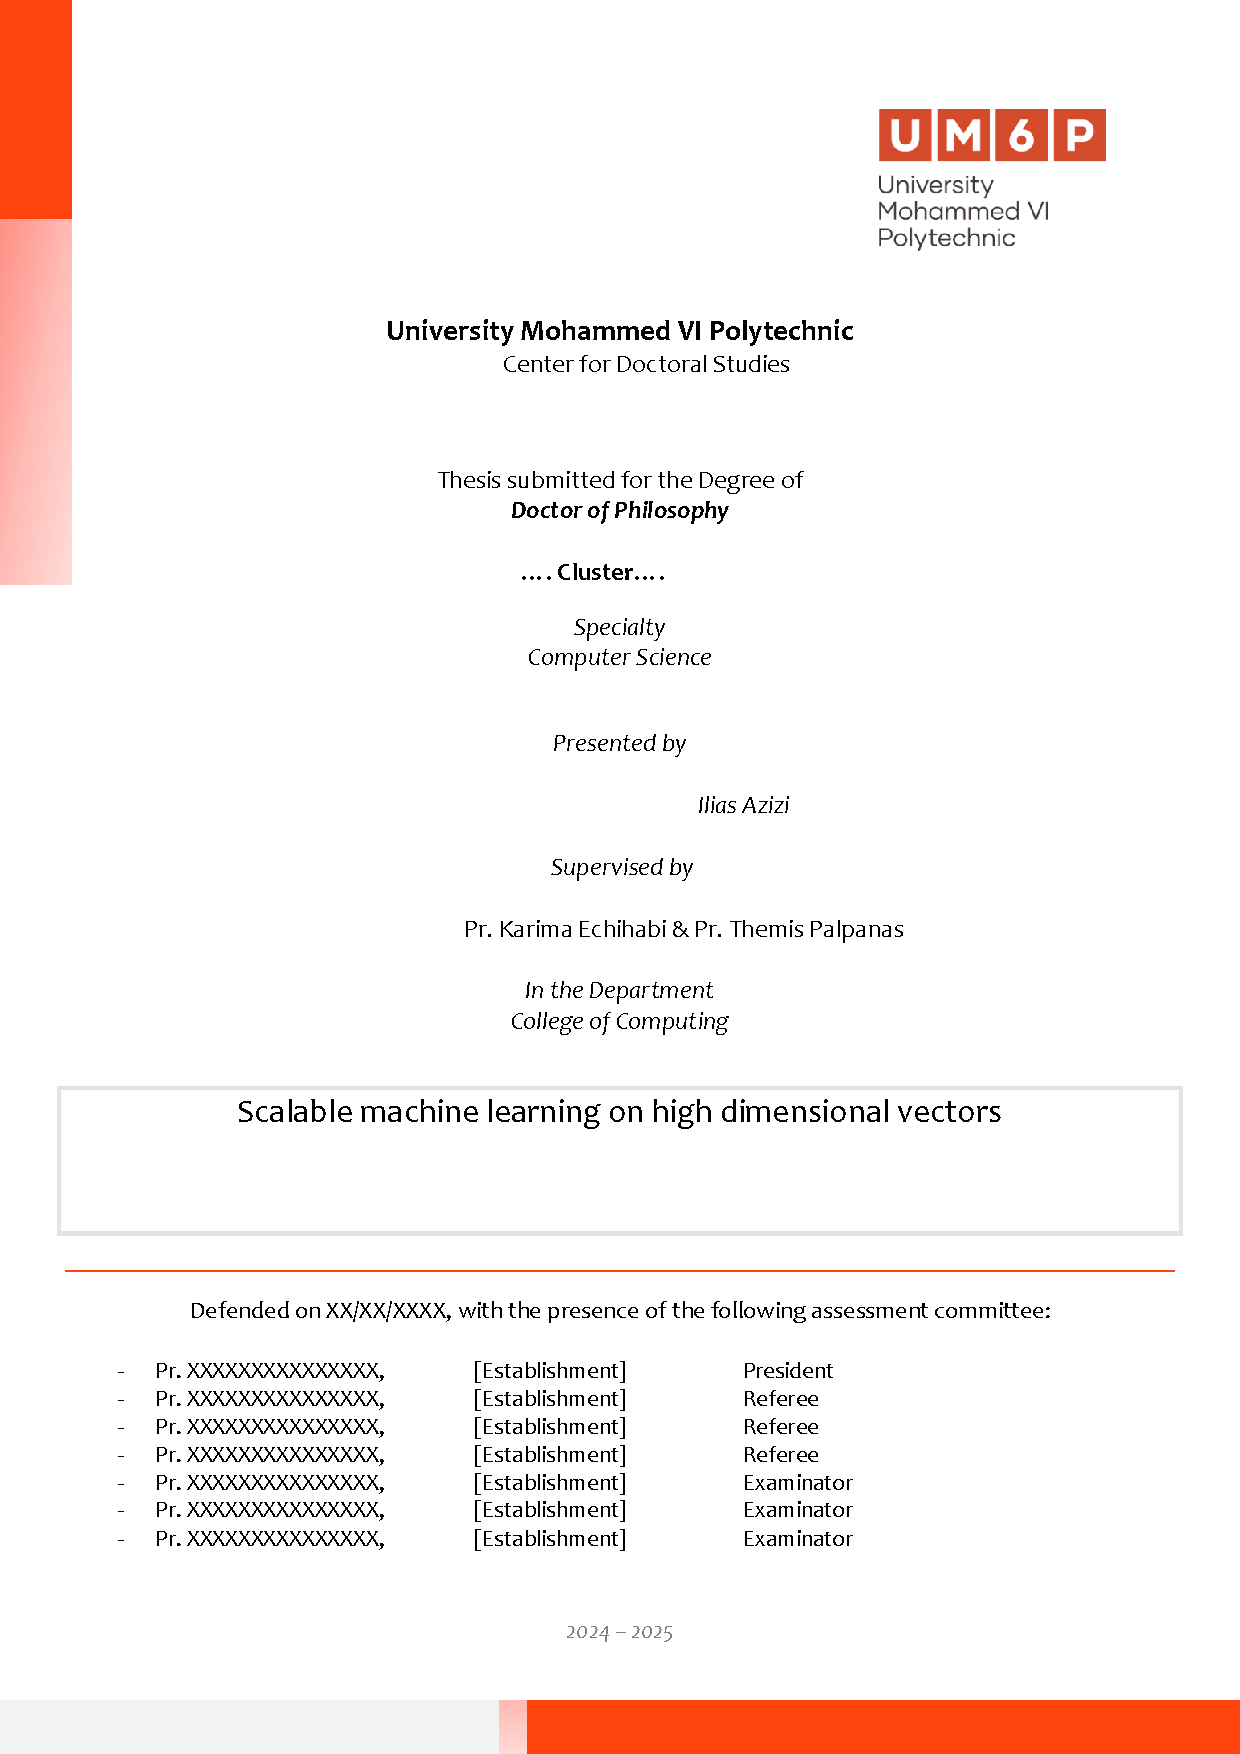
\includepdf[pages=-]{../img/page.pdf}

\begin{titlepage}
    \centering
    \vspace*{3cm} % Adjust vertical space

    {\Huge \textbf{Thesis Manuscript}\\}
    \vspace{1.5cm}

    {\LARGE Scalable High-Dimensional Vector Similarity Search\\}

    \vfill

    {\Large \textbf{Presented by:} \\ \Large Ilias Azizi}

    \vspace{1.5cm}

    {\Large University Mohammed VI Polytechnic\\
    College of Computing\\
    Morocco}
    \vspace{1cm}

    {\Large University Paris Cité\\
    Laboratoire d'Informatique Paris Descartes\\
    France}
    \vspace{1cm}

    {\Large \textbf{2023 - 2024}\\}
    
\end{titlepage}


\clearpage

\begin{abstract}
The unprecedented increase in high-dimensional data across sectors like agriculture, healthcare, cybersecurity, seismology, and finance has led to an urgent demand for sophisticated analytical systems capable of processing and exploring large datasets. These datasets, often reaching terabytes in size and involving hundreds or thousands of dimensions, require advanced tools to detect valuable patterns and derive insights.

Vector search is a fundamental operation in numerous data science applications, such as data integration, recommendation systems, large language models, and information retrieval. In these tasks, data such as images, text, or videos are represented as vectors in a high-dimensional space, and the objective is to find the closest object(s) to a query within large collections of vectors. However, as these collections grow exponentially in both size and dimensionality, performing such searches becomes increasingly complex. Although both exact and approximate vector search methods have been developed, they struggle to efficiently scale to the size of today's massive datasets. Traditional techniques, including tree-based and hash-based approaches, have become impractical for handling large-scale vector data collections.
%containing millions or even billions of high-dimensional vectors.

In recent years, graph-based methods have emerged as a promising alternative for managing large-scale vector search tasks. These methods construct a graph where each node represents a data object, and edges link the most similar objects, leading to improved query efficiency. Nevertheless, despite their advantages, existing graph-based approaches face critical challenges, including (i) a lack of indexing scalability on large datasets, and (ii) low query accuracy on hard datasets and query workloads.

%including (i) scalability when handling vast data collections and (ii) maintaining accuracy on difficult datasets.

This thesis presents several key contributions: (i) the design of a novel scalable approach for in-memory, ng-approximate graph-based vector search that efficiently indexes and searches large datasets by leveraging both tree and graph index structures; (ii) an exhaustive evaluation of state-of-the-art graph-based methods on large-scale datasets, along with the introduction of a new taxonomy that classifies graph-based vector search techniques according to five key paradigms; (iii) a novel merging strategy that combines tree and graph indexes to achieve high performance in both latency- and throughput-optimized settings; and (iv) the development of a new graph-based method that optimizes the indexing and searching of large-scale vector datasets; 

Through these contributions, this thesis aims to advance the scalability and accuracy of graph-based vector search algorithms in large-scale data collections, laying a strong foundation for further research on graph structures for vector search.
\end{abstract}

%\begin{acknowledgements}
	
%Add acknowledgements here.

%\end{acknowledgements}

\section*{Acknowledgments}

First and foremost, I am profoundly grateful to God for His blessings, guidance, and strength throughout this journey.

I wish to express my deepest appreciation to my co-supervisors, Prof. Karima Echihabi and Prof. Themis Palpanas, for their unwavering support, encouragement, and insightful guidance. Their expertise and mentorship have been instrumental in the completion of this thesis.

My heartfelt gratitude goes to my family for their unconditional love and support. To my father Ahmed, my beloved wife Diana, my sister Asma, my brothers Anas and Fadlallah—your encouragement and understanding have been my pillars of strength. This work would not have been possible without you.

I dedicate this thesis to the memory of my mother, Habiba, who left us in June 2010. Her love and teachings continue to inspire me every day. I also remember all my departed family members, whose memories motivate me to strive for excellence.

I am sincerely thankful to my dear friends Waiel, Mouna, Mouad, Mohamed, Abdel, Amine, Aissame and all others who have stood by me with their support and camaraderie.

Special thanks to my colleagues from the DMG team at the College of Computing, Mohammed VI Polytechnic University and the DiNo team at the University of Paris Cité. I am grateful for the collaborative environment and the enriching discussions we shared. I also extend my appreciation to the faculty and administrative staff of both universities for their assistance and support.

I would like to acknowledge the UM6P African Supercomputing Center and its support team for providing the computational resources and technical assistance necessary for conducting our experiments and workloads.

Finally, to everyone who has contributed to this journey, whether mentioned here or not, your support has been invaluable, and I am deeply appreciative.


\tableofcontents

\end{preliminary}


\listoffigures
\listoftables

\graphicspath{{../img/intro/}}

\chapter{Introduction}
The rapid proliferation of data across various domains and artificial intelligence applications has led to an explosion of high-dimensional datasets. As these collections grow, encompassing millions or even billions of data points, the challenge becomes how to efficiently process, analyze, and retrieve relevant information. Many data-driven applications, from machine learning models to recommendation systems, rely on effective interaction with these datasets to extract insights and knowledge on demand, with vector search being a core operation.

While traditional vector search approaches such as tree-based and hash-based methods attempt to execute this task efficiently, they often fail to deliver satisfactory performance at scale. Over the last decade, graph-based methods have emerged as a leading solution for efficient vector search, offering high recall and impressive query efficiency. However, existing graph-based structures still face significant challenges when it comes to scaling efficiently to massive collections.

This thesis addresses these challenges by proposing novel methods that advance the state of the art in high-dimensional similarity search. We introduce ELPIS, a new approach for in-memory ng-approximate high-dimensional vector search that leverages both tree and graph structures, combining their strengths to overcome mutual limitations and outperform state-of-the-art methods in terms of latency, while offering competitive throughput. Additionally, we propose a new taxonomy that categorizes state-of-the-art graph-based approaches according to key paradigms, providing insights into the strengths and weaknesses of each. Finally, we present a novel graph-based approach that improves indexing scalability and query performance over existing methods.

In this chapter, we first provide an overview of the similarity search problem and the main data types addressed in this work, followed by a summary of the key contributions of this thesis.
\clearpage 

%\section{Problem Overview}
\section{Overview}
\label{sec:overview}
Vector search is a backbone operation at the core of many essential data analytics tasks. It supports recommendation~\cite{conf/kdd/wang2018,amazon}, 
information retrieval~\cite{conf/williams2014}, clustering~\cite{journal/JMLR/bubeck2009,journal/pattrecog/Warren2005}, 
classification~\cite{classification,pros},
and anomaly detection~\cite{discord,norma,series2graph,landmines,nba,landmines,DBLP:journals/datamine/LinardiZPK20,DBLP:journals/pvldb/BoniolPPF21,DBLP:journals/pvldb/PaparrizosKBTPF22,DBLP:journals/pvldb/PaparrizosBPTEF22} across various scientific and business domains, including bioinformatics~\cite{biof1,biof2}, 
computer vision~\cite{cv1,cv2}, 
security~\cite{cybersecurity,cyb2}, 
finance~\cite{finance1,finance2}, 
and 
medicine~\cite{medcine1,medicin2}. 
In data integration, similarity search plays a crucial role in entity resolution~\cite{journal/pvldb/ebraheem2018}, completion of missing value~\cite{retro}, and data discovery~\cite{journal/pvldb/zhu2016}. Furthermore, it is widely used in software engineering~\cite{journal/pacml/uri2019,conf/icsec/nguyen2016} for monitoring I/O usage and automating API mappings, as well as in cybersecurity for profiling network activity and detecting malware~\cite{cybersecurity,cyb2}. More recently, similarity search has become increasingly vital in enhancing the performance and interpretability of large language models (LLMs), helping reduce hallucinations in generated content~\cite{retrieval-diffusion-models,dense-passage-retrieval,seq2seq,rag-nlp,rag0,rag1,rag2,rag3}.

The vector search problem has been extensively studied over the past 30 years~\cite{hnsw,hercules,rng,hydra1,hydra2} under various terminologies, including similarity search, or often reduced to the k-Nearest Neighbors (k-NN) problem~\cite{conf/icde/echihabi2021,conf/sigmod/echihabi2020,gogolou2019progressive}, and as high-dimensional data collections continue to grow at unprecedented rates, the need for efficient and optimized vector search solutions has garnered increasing attention.

This problem can be abstracted as finding the most similar object(s) from a collection of objects based on a similarity measure, K nearest neighbors~\cite{conf/sigmod/echihabi2020, aumuller2017ann,ann-benchmark-journal}. These objects can represent text, images, videos, graphs, data series, database tables, or learned representations, which are ultimately encoded as vectors in a vector space~\cite{hydra1,hydra2,DBLP:conf/edbt/EchihabiZP21,conf/sigmod/echihabi2020}. The similarity measure, such as Euclidean distance~\cite{euclid}, is used to identify the objects with the closest representations to a given query object.

Different variants of this problem exist. Depending on the required level of accuracy, a similarity search can either be exact, where the objective is to return the exact closest objects to the query from the dataset~\cite{hercules,hydra1,conf/icde/echihabi2021,messi,parisplus,dumpy,dpisax,kdtree,dstree,isax2+,ulisse,vafile,twinsubsequences,oddysey,dstree}, or approximate, where accuracy is traded for faster and less resource-intensive responses~\cite{hydra2,hercules,qalsh,kdtree,kgraph,efanna,hnsw,dpg,conf/icassp/jegou2011,journal/iccv/xia2013,journal/pami/babenko15,hnsw,hcnng,nsg,vamana}. The approximate problem can further be categorized into two main classes: Approximate similarity search with guarantees on error bounds\cite{conf/vldb/lv2007,sk-lsh,journal/pvldb/zheng2020,journal/pvldb/zhu2016,conf/stoc/indyk1998,conf/vldb/sun14,qalsh,hydra2,srs,conf/sigmod/gogolou20}, and Approximate similarity search with no guarantees on error bounds, namely $ng$-Approximate, where faster performance is prioritized over error bounds ~\cite{kdtree,hydra2,elpis,hercules,hnsw,nsg,hcnng,efanna,nsg,nssg,nsw11,vamana,ieh,dpg,kgraph}.

With the recent rise of AI applications~\cite{rag0, nsg,alibabaknngml, recommender_systems,faiss,amazon}, ng-approximate similarity search has gained more attention, particularly since many AI applications do not require exact responses for k-NN queries. These applications can achieve satisfactory results with medium accuracy, ensuring reasonable response times. Examples include recommendation systems~\cite{conf/kdd/wang2018,amazon,nsg}, image search engines~\cite{nsg,faiss}, and Retrieval-Augmented Generation (RAG) models\cite{retrieval-diffusion-models,dense-passage-retrieval,seq2seq,rag-nlp}, which combine large language models with vector search engines to efficiently retrieve relevant context ~\cite{retrieval-diffusion-models,rag-nlp,rag0,rag1,rag2,rag3}. This integration helps generate more accurate and up-to-date query responses, reinforcing the critical role of vector search in modern AI applications.

Existing solutions for $ng$-approximate vector search can be categorized to three main classes: Tree-based indexing methods partition the dataset space into embedded hierarchical sub-spaces using a tree data structure, where similar data points belong in the same leaves~\cite{va+file,dstree,isaxfamily,hercules,oddysey,isax2+,isax2plus}.
Hash-based indexing methods map the dataset vectors into different buckets of hash codes using multiple hash tables, and guarantee with high probability that similar data are hashed into the same buckets~\cite{lsh-survey,qalsh,aumuller2017ann,flann,sk-lsh}. 
Graph-based indexing methods structure the dataset into a proximity graph, where data points are represented as vertices and each vertex is connected to a set of similar vertices~\cite{kgraph,ieh,efanna,nsw11,nsw14,hnsw,nsg,nssg,vamana,SPTAG1,SPTAG3,elpis,dpg,graph-survey-vldb,lshapg}.

Each of the three families of similarity search methods has its advantages and disadvantages~\cite{hydra2,elpis}. 
Tree-based techniques are efficient at index building with a new class of extensions~\cite{hydra2} supporting all three flavors of search: exact, $\delta$-$\epsilon$-approximate and $ng$-approximate search. These extensions achieve the best performance on all scenarios except on $ng$-approximate search, where their efficiency is still unsatisfactory for many real applications~\cite{hydra2,hydra1,conf/sigmod/echihabi2020,DBLP:conf/edbt/EchihabiZP21,conf/icde/echihabi2021}. 
Hash-based techniques support $\delta$-$\epsilon$-approximate search with additional theoretical guarantees on query efficiency, but are not scalable due to the high index construction time, high memory footprint and low empirical search performance. 
Theoretical guarantees on accuracy are provided on the distance approximation error, but this does not always translate into good recall empirically~\cite{hydra2,aumuller2017ann,lsh-survey,DBLP:conf/edbt/EchihabiZP21,conf/icde/echihabi2021,qalsh,elpis}. 
Graph-based methods offer the best performance in practice for $ng$-approximate search, but building the graph structure on large datasets is extremely expensive both in time and space~\cite{elpis,aumuller2017ann,conf/sigmod/echihabi2020,hydra2,graph-survey-vldb}. 
Moreover, such techniques do not offer any guarantees on search quality and efficiency. 
Despite these disadvantages, graph-based approaches remain the methods of choice for many real applications such as recommendation systems~\cite{graphrec2,graphrec1,alibabaknngml,DBLP:journals/corr/JohnsonDJ17} that require a very low query latency (a few milliseconds per query on billion-scale collections), and can tolerate a lack of theoretical guarantees on the quality of the answers as long as a high recall ($\ge$ 0.90) can be achieved empirically.  


\begin{figure}[tb] 
\centering
		\captionsetup{justification=centering}
		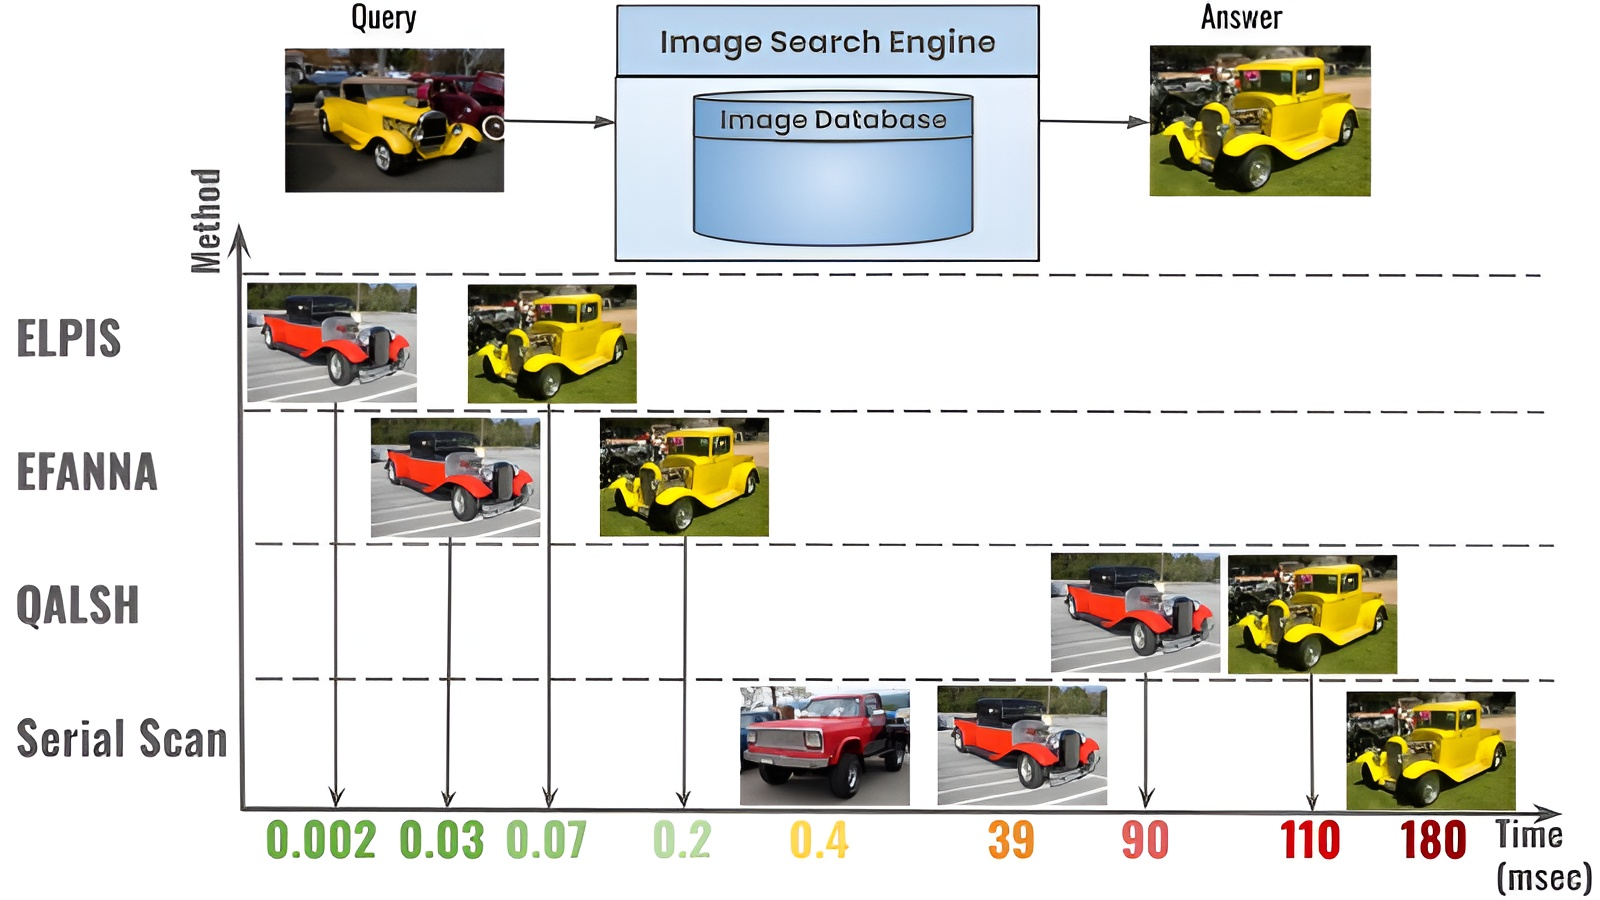
\includegraphics[width=0.8\columnwidth]{../img/intro/ENDTOENDEXAMPLE2.png}
		\caption{
  Image retrieval using different vector search methods.
  }        
		\label{fig:use_case}
 \end{figure}


Figure~\ref{fig:use_case} illustrates vector search in an image retrieval use case. We produce embeddings for ImageNet~\cite{imagenet} using a ResNet50 model~\cite{resnet}. 
We report the time at which a best-so-far (bsf) answer is found (i.e., the image in the database most similar to the query) by vector search techniques from different families: ELPIS~\cite{elpis} and EFANNA~\cite{efanna} for ng-approximate search, QALSH~\cite{qalsh} for $\delta$-$\epsilon$-approximate search, and a serial scan for exact search. 
Each row shows the bsf answer returned by each method (y-axis) at a given timestamp (x-axis). We observe that the graph-based approach  ELPIS returns the same answer as the serial scan and hash-based approach QALSH over three orders of magnitude faster, which explains the popularity of graph-based vector search in many real applications; We also point that not all graph-based methods have the same performance, e.g. ELPIS is 3x faster than EFANNA, 


\section{Main Contributions}
\label{sec:contributions}
Our main contributions are as follows:

\textbf{1. ELPIS: A Scalable Graph-based In-memory Vector Search }  
This thesis introduces \textit{ELPIS}, a novel framework for in-memory \textit{ng}-approximate high-dimensional vector search that combines the strengths of tree-based and graph-based indexing structures. By leveraging the hierarchical organization of trees and summarization of EAPCA-Tree for scalability and the efficiency of graph-based methods for query latency, ELPIS addresses the shortcomings of both approaches. It significantly reduces query latency while maintaining competitive accuracy, even in large-scale datasets comprising billions of high-dimensional vectors. The approach enables ELPIS to scale efficiently with increasing data sizes, making it suitable for modern data-driven applications that require both high speed and accuracy. In extensive evaluations, ELPIS consistently outperforms existing state-of-the-art methods, particularly in latency-sensitive environments.

\textbf{2. Comprehensive Survey and Taxonomy of Graph-Based Search Methods} 
A major contribution of this work is a detailed survey of graph-based similarity search techniques. This survey offers a systematic evaluation of current methods and proposes a new taxonomy that categorizes these approaches into five key paradigms. The taxonomy provides an organized framework for understanding the variety of graph-based methods, clarifying their respective strengths and limitations. This contribution offers researchers and practitioners valuable insights into selecting the most appropriate method for specific applications, while also identifying areas for future exploration. This survey serves as a foundational reference for the community, highlighting challenges in scaling and optimizing graph-based similarity search for increasingly large and complex datasets.

\textbf{3. Throughput Optimization via EAPCA-Based Merging}  
This thesis introduces a novel EAPCA-based merging technique that effectively addresses the throughput limitations of ELPIS. By utilizing Extended Adaptive Piecewise Constant Approximation (EAPCA) lower-bounding distances, the merging process intelligently combines smaller, latency-optimized graphs into larger, throughput-optimized structures. This selective merging approach significantly reduces redundant distance computations during query processing, allowing for more efficient traversal of the vector space. As a result, ELPIS is capable to efficiently balance between latency- and throughput-optimized performance, providing a robust solution for large-scale vector search tasks without the need to build separate indexes optimized for each scenario.

\textbf{3. OIGAS: Optimized Incremental Insertion-based Graph for Efficient Vector Search}  
Expanding upon the findings from the survey, this thesis proposes a novel graph-based search algorithm designed to improve both indexing scalability and query efficiency. The new approach optimizes graph indexing by reducing the required computation to incrementally construct the graph index structures, as well as proposing a combined strategies for pruning edges within the graph based on node in-degree, allowing it to handle large datasets more efficiently than existing techniques. This advancement provides a significant improvement over traditional methods, particularly in scenarios that require a fast indexing of the large collection of data with minimum loss in answer quality during search.


The contributions of this thesis have led to the following publications:

1. Ilias Azizi, Karima Echihabi, Themis Palpanas. Elpis: Graph-Based Similarity Search for Scalable Data Science. Proceedings of the VLDB Endowment 16.6 (2023): 1548-1559.~\cite{elpis}

2. Ilias Azizi, Vector Search on Billion-Scale Data Collections. In VLDB PhD Workshop, 2024.~\cite{iazizi2024}

3. Ilias Azizi, Karima Echihabi, Themis Palpanas. Graph-Based Vector Search:
An Experimental Evaluation of the State-of-the-Art. Proceedings of the ACM on Management of Data (2025).~\cite{gass}

The following contributions are part of ongoing research and are in preparation for future publication:

4. Ilias Azizi, Karima Echihabi, Themis Palpanas. ELPIS+: Optimized Throughput Vector Search over Billion-scale Data Collections. 

5. Ilias Azizi, Karima Echihabi, Themis Palpanas. OIGAS: Optimized Incremental Insertion based Graph for Efficient Vector Search. 

\section{Outline}
The rest of the thesis is organized in 7 chapters. Chapters 2 and 3 lay the foundational background on high-dimensional similarity search, surveys the different families of methods (i.e., tree-based, hash-based, and graph-based), and discusses their strengths and limitations. Chapter 4 introduces a comprehensive taxonomy and analysis of graph-based similarity search methods, evaluating them based on their construction techniques, edge selection strategies, search mechanisms, and scalability. Chapter 5 presents the ELPIS Framework, a hybrid method that integrates tree-based and graph-based structures to optimize both latency and throughput in vector search tasks. Chapter 6 focuses on ELPIS Merging, a novel technique that enhances throughput through an EAPCA-based graph merging approach, providing efficient scalability for billion-scale datasets. Chapter 7 introduces OIGAS, an innovative graph-based method designed for incremental insertion and query performance optimization in dynamic datasets. Each of these chapters includes detailed performance evaluations and comparisons with state-of-the-art methods, supported by experimental results and plots. Finally, Chapter 8 concludes the thesis by summarizing the main contributions and outlining future research directions.

\graphicspath{{../img/problem/}}
\chapter{Preliminaries}
\label{chapter:problem}

\section{Introduction}
The exponential growth of high-dimensional vector across various domains, including medicine, cybersecurity, and e-commerce, has intensified the need for efficient data analysis and retrieval. In this context, vector search, a core operation used in applications such as recommendation systems, classification, and clustering, becomes a critical bottleneck. With datasets often consisting of millions or billions of vectors in high-dimensional spaces, efficiently finding the nearest neighbors (i.e., the most similar objects to a given query) has emerged as a fundamental challenge.

In this chapter, we provide definitions for the different flavors of vector search, including data type, similarity measures, queries, and methods. 
\clearpage

\section{Definitions}
\label{sec:definitions}

\subsection{Data Types}
In the context of similarity search, complex objects are typically represented as points in an \(d\)-dimensional space, often referred to as vectors, thus vector search. 

 A \textbf{vector} is an element in a \(d\)-dimensional real space, represented as \(V = [v_1, v_2, \dots, v_d] \in \mathbb{R}^d\), where each \(v_i\) is a component corresponding to a specific feature or attribute. In similarity search, each object from a dataset \(S = \{V_1, V_2, \dots, V_n\}\) is mapped to a vector in \(\mathbb{R}^d\), with each vector \(V\) representing an object ~\cite{vector}.

%\ilias{add embed       dings vs learned embeddings}

Various methods can be used to map objects into vectors, depending on the type of data being processed. Recently, machine learning techniques such as CNNs~\cite{cnn,cnn1}, RNNs~\cite{rnn,rnn1}, Graph Neural Networks ~\cite{gnn,gnn1}, and, more recently, transformers~\cite{transf,transf1,transf2,transf3}, have been widely used to represent objects in vectorial space by learning embeddings that capture the underlying features of these objects. These learned embeddings often provide richer and more flexible representations, adapting to the complexity of the data~\cite{lemb,lemb1}.

For instance, in image search, traditional methods relied on handcrafted descriptors like SIFT~\cite{sift,sift1}, HOG~\cite{hog}, or SURF~\cite{surf}, which extracted specific visual features (e.g., edges, corners, textures) to represent images as feature vectors. However, modern deep learning models, particularly transformers and  convolutional neural networks~\cite{cnn,cnn1, transf1,transf2}, have replaced these descriptors by automatically learning hierarchical feature representations that are more robust to variations in scale, lighting, and orientation~\cite{lemb1,cnn2,lemb,transf}. This shift has dramatically improved the performance of similarity search tasks in image retrieval~\cite{amazon,faiss,nsg,aumuller2017ann}.

Similarly, in natural language processing (NLP), traditional approaches represented text using techniques like bag-of-words or TF-IDF, which lacked semantic understanding \cite{Manning2008}. With the advent of word embeddings such as Word2Vec \cite{Mikolov2013}, GloVe \cite{Pennington2014}, and more advanced transformer-based models like BERT \cite{Devlin2019} and GPT \cite{Radford2018}, text is now encoded into dense vector representations that capture semantic relationships, allowing for more accurate similarity searches based on meaning rather than mere word frequency

In the case of graph-structured data, Graph Neural Networks (GNNs) have gained popularity for encoding nodes and their relationships into vectors that can be used for tasks such as link prediction, node classification, and graph similarity search \cite{Scarselli2009, Kipf2017, Hamilton2017}. These learned representations take into account both node features and graph topology, outperforming traditional handcrafted approaches.

Compared to earlier methods that relied on predefined descriptors \cite{Lowe2004, Dalal2005}, these machine learning-driven vector representations allow for more dynamic, context-aware similarity search \cite{Krizhevsky2012, Mikolov2013a}, enabling better generalization across different data types and improved performance on large-scale, real-world datasets. The transition to using learned embeddings has not only enhanced the quality of similarity search but also paved the way for dealing with complex, multi-modal datasets \cite{Ngiam2011, Radford2021}, where different data types (e.g., images, text, graphs) can be embedded into a unified vector space for cross-domain retrieval.
In this thesis, we primarily focus on two common data types: images and data series, both of which are crucial in high-dimensional vector search applications.

\paragraph{Images} 
Images are represented as multi-dimensional arrays of pixel values, typically corresponding to spatial information in grayscale or RGB channels. For computational tasks, these raw images are often transformed into vectorized forms. This transformation can be achieved through hand-crafted descriptors, such as SIFT \cite{Lowe2004} or HOG \cite{Dalal2005}, which capture specific visual features like edges, textures, and shapes. Alternatively, deep learning models, such as transformers \cite{transf,transf1,transf2,transf3, Vaswani2017} and convolutional neural networks \cite{LeCun1998, Krizhevsky2012,cnn,cnn1,cnn2}, generate embeddings by learning hierarchical feature representations directly from the data. Both approaches enable images to be represented as vectors in a high-dimensional space, facilitating tasks like classification, retrieval, or similarity comparison.

\paragraph{Data Series} 

A data series is a sequence of data points indexed by a continuous domain, such as time, space, depth, or frequency ~\cite{KostasThemisTalkICDE,conf/icde/echihabi2021,Lin2003, Keogh2005}. Formally, a data series can be represented as a vector \( V \in \mathbb{R}^d \), where \(d\) is the dimensionality of the series and each component \(v_i\) corresponds to a specific point in the domain~\cite{Shieh2009}.. Given a dataset \( S = \{V_1, V_2, \dots, V_n\} \) of \(n\) data series vectors in \( \mathbb{R}^d \), the task of similarity search is to find the vectors \(V \in S\) that are most similar to a query vector \( Q \in \mathbb{R}^d \) based on a defined distance measure~ \cite{conf/sigmod/echihabi2020,Palpanas2019,palpanas2015data,Faloutsos1994, Keogh2002}.

\subsection{Distance Measures}

Measuring the \textbf{similarity} or \textbf{dissimilarity} between vectors \(Q\) and \(V\) in the dataset \(S\) is critical for identifying the nearest neighbors. Distance functions quantify how close these vectors are in \(\mathbb{R}^d\), with \textbf{Euclidean distance}~\cite{euclid} being the primary metric of focus in this thesis.

\begin{definition}[Minkowski Distance]
    The Minkowski distance generalizes multiple distance metrics, defined for vectors \(Q\) and \(V\) in \(\mathbb{R}^d\) as:
    \begin{equation}
        \mathcal{D}_p(Q, V) = \left( \sum_{i=1}^{d} |q_i - v_i|^p \right)^{1/p}
        \label{eq:minkowski_distance}
    \end{equation}
    where \(p \geq 1\), and \(q_i\) and \(v_i\) are the \(i\)-th components of vectors \(Q\) and \(V\), respectively. The Minkowski distance encompasses both \textbf{Euclidean} and \textbf{Manhattan} distances, depending on the value of \(p\).
\end{definition}

\begin{definition}[Euclidean Distance]
    The Euclidean distance is a special case of the Minkowski distance when \(p = 2\), and is defined as:
    \begin{equation}
        \mathcal{D}_E(Q, V) = \sqrt{\sum_{i=1}^{d} (q_i - v_i)^2}
        \label{eq:euclidean_distance}
    \end{equation}
    This metric measures the straight-line (geometric) distance between vectors \(Q\) and \(V\) in \(\mathbb{R}^d\). Euclidean distance is the most widely used metric in high-dimensional similarity search, and it is the focus of this thesis.
\end{definition}

\begin{definition}[Manhattan Distance]
    The Manhattan distance, also known as the L1 distance, is another special case of the Minkowski distance when \(p = 1\), and is defined as:
    \begin{equation}
        \mathcal{D}_1(Q, V) = \sum_{i=1}^{d} |q_i - v_i|
        \label{eq:manhattan_distance}
    \end{equation}
    This metric sums the absolute differences between the corresponding components of the vectors.
\end{definition}

\begin{definition}[Cosine Similarity]
    Cosine similarity measures the cosine of the angle between two vectors \(Q\) and \(V\) in \(\mathbb{R}^d\), and is defined as:
    \begin{equation}
        \mathcal{S}_{\text{cosine}}(Q, V) = \frac{Q \cdot V}{\|Q\| \|V\|}
        \label{eq:cosine_similarity}
    \end{equation}
    where \(Q \cdot V\) represents the dot product, and \(\|Q\|\) and \(\|V\|\) are the Euclidean norms of \(Q\) and \(V\). Cosine similarity is commonly used in cases where the orientation of the vectors is more important than their magnitude, such as in text similarity or high-dimensional embeddings.
\end{definition}

\paragraph{Focus on Euclidean Distance}
In this thesis, we primarily focus on the \textbf{Euclidean distance} (\(\mathcal{D}_E(Q, V)\)) measure, since it is used extensively in modern
%for high-dimensional similarity search tasks
applications~\cite{Indyk1998, Datar2004,vamana,ngt_library,zhang2018visual,spfresh}  because it is simple and computationally efficient~\cite{Arya1998}. For all subsequent discussions, the Euclidean distance will be denoted as \(\mathcal{D}(Q, V)\).
%, making it a practical choice for large-scale datasetss 

%\section{Similarity Search Problem}
\section{Problem Statement}
\label{sec:similarity_search}

In the context of high-dimensional vector search, the similarity search problem involves finding the most similar objects in a dataset \(S = \{V_1, V_2, \dots, V_n\} \subseteq \mathbb{R}^d\) to a given query vector \(Q \in \mathbb{R}^d\), using a distance function \(\mathcal{D}(Q, V)\). This search can be classified into two types: \textbf{exact} and \textbf{approximate}.

\subsection{Exact Similarity Search}
In exact similarity search, the objective is to retrieve the \(k\)-nearest neighbors (k-NN) of the query \(Q\). The exact solution retrieves a set \(A = \{V_1, V_2, \dots, V_k\} \subseteq S\) such that:
\begin{equation}
    \mathcal{D}(Q, V_i) \leq \mathcal{D}(Q, V_j) \quad \forall V_j \in S \setminus A
    \label{eq:exact_knn}
\end{equation}
This ensures that the vectors in \(A\) are the exact closest vectors to \(Q\) according to the distance metric \(\mathcal{D}\), with no error in proximity.

\subsection{Approximate Similarity Search}
Approximate similarity search aims to trade off some accuracy for faster performance. These methods can be divided into two categories:

\paragraph{Guaranteed Approximation}
In \(\epsilon\)-approximate search, the result guarantees that the distance between the query \(Q\) and the retrieved vector \(V\) is at most \((1 + \epsilon)\) times the distance to the exact nearest neighbor:
\begin{equation}
    \mathcal{D}(Q, V) \leq (1 + \epsilon) \cdot \mathcal{D}(Q, V_{\text{exact}})
    \label{eq:approx_knn_guarantee}
\end{equation}
where \(V_{\text{exact}}\) is the exact nearest neighbor of \(Q\). This guarantee ensures that the error is bounded by the factor \(\epsilon\), offering a controlled approximation with a trade-off between speed and accuracy.

\paragraph{Non-Guaranteed Approximation}
In non-guaranteed ($ng$) approximate search, there is no strict error bound on the proximity of the retrieved vectors to the query \(Q\). These methods focus on providing fast responses by reducing the computational complexity of the search process, often using heuristic-based approaches to retrieve vectors that are close to \(Q\), but without any formal guarantees on their accuracy. This approach is particularly suited for large-scale datasets where exact or guaranteed approximate searches are computationally expensive.

\paragraph{Focus of this Thesis}
In this thesis, we primarily focus on \textbf{$ng$-approximate similarity search}, which is effective for large-scale, high-dimensional datasets~\cite{hydra2, aumuller2017ann, conf/icde/echihabi2021,elpis,hnsw,neurips-2021-ann-competition}. The terms \textit{approximate similarity search}, \textit{approximate vector search}, and \textit{$ng$-approximate similarity search} will be used interchangeably throughout this work.


\section{Conclusion}
In the following chapters, we will explore various approximate similarity search methods, with a particular focus on in-memory graph-based approaches. Chapter 3 will introduce different classes of approximate similarity search methods, along with a novel taxonomy for graph-based approaches, outlining new key paradigms. Chapter 4 will present our new approach for single-query search, ELPIS. Chapter 5 will demonstrate how ELPIS can be adapted to optimize throughput and remain competitive in answering multiple queries in parallel across large-scale data collections, using a novel graph-merging strategy. In Chapter 6, we will introduce OIGAS, a graph-based approach designed for efficiently indexing and searching large-scale datasets.
\graphicspath{{../img/related/}}
\chapter{Related Work}
\label{chapter:related}
The vector search problem has been extensively studied for over fifty years, with proposed solutions based on a variety of data structures, including \textit{scans}, \textit{trees}, \textit{hashing}, \textit{graphs}, and \textit{inverted indexes}. Early approaches, such as brute-force scans, suffer from high computational costs, making them impractical for large datasets~\cite{vafile}. \textit{Tree-based methods} (e.g., kd-trees) and \textit{hashing techniques} (e.g., Locality-Sensitive Hashing) improve search efficiency but face limitations, particularly in high-dimensional spaces~\cite{dstree,isax2+,conf/stoc/indyk1998,qalsh}.

In recent years, \textit{graph-based methods} have gained prominence due to their ability to achieve low query latency and high recall, making them suitable for large-scale applications~\cite{hnsw,vamana,nsg}. \textit{Hybrid approaches} that combine multiple data structures have also emerged, optimizing the balance between search accuracy and efficiency~\cite{ieh,elpis}.

This chapter explores the existing families of approximate similarity search methods, including tree-based~\cite{dstree,isax2+,flann}, hash-based~\cite{conf/stoc/indyk1998,qalsh}, graph-based~\cite{hnsw,nsg,vamana}, and hybrid methods~\cite{ieh,elpis}. 
\clearpage

\section{Approximate Similarity Search}
\label{sec:related_works}

In vector search, the goal is to retrieve vectors from a dataset \(\mathbb{S}\), consisting of \(n\) vectors in \(\mathbb{R}^d\), that are most similar to a query vector \(V_Q\). The most basic method, known as brute-force or sequential search, involves comparing \(V_Q\) with every vector in \(\mathbb{S}\), which has a time complexity of \(O(nd)\). As the size of the dataset \(n\) and dimensionality \(d\) grow, this approach becomes impractical for large-scale, high-dimensional data.

\begin{figure}[ht] 
\centering
		\captionsetup{justification=centering}
		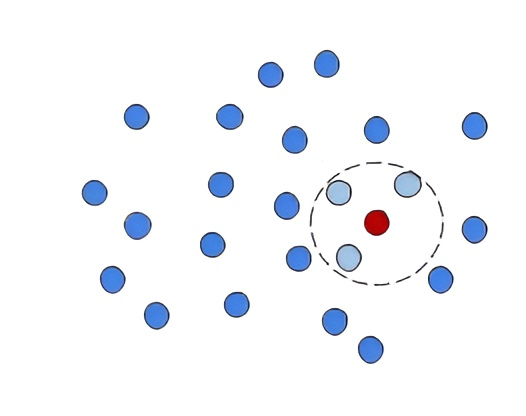
\includegraphics[width=0.5\columnwidth]{../img/related/knn.jpg}
		\caption{Brute-force retrieval of 3-Nearest Neighbors (light blue) for a query vector (red) from the dataset (blue)}        
		\label{fig:KNN_retrieval}
\end{figure}

To address this inefficiency, modern techniques focus on either reducing the dimensionality \(d\) through summarization or decreasing the number of comparisons by leveraging efficient indexing structures. These indexing structures prune unnecessary comparisons to \(V_Q\), thereby significantly improving performance. While some methods guarantee exact results, others aim for approximate answers—either with theoretical guarantees like \(\epsilon\)-approximations, or practical but non-guaranteed approaches, such as ng-approximation.

\noindent{\textbf{Summarization Techniques:}} Summarization techniques are fundamental to improving the efficiency of approximate similarity search by reducing the dimensionality of high-dimensional vectors, thus enabling faster search over large datasets. These methods attempt to transform or compress vectors into lower-dimensional representations while maintaining their key structural properties, speeding up the search while keeping accuracy loss to a minimum.

\begin{figure}[ht] 
\centering
		\captionsetup{justification=centering}
		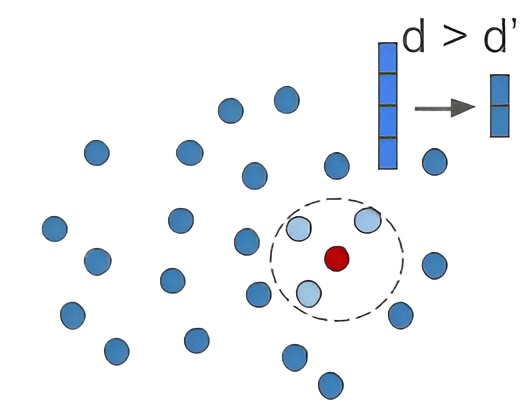
\includegraphics[width=0.5\columnwidth]{../img/related/sumb.jpg}
		\caption{Retrieval of 3-Nearest Neighbors (light blue) for a query vector (red) from the dataset (blue) summarized in lower dimensions}        
		\label{fig:sum_retrieval}
\end{figure}

For high-dimensional vectors, one of the most well-known summarization methods is \textit{Quantization}, which compresses continuous vector values into a finite set of codewords stored in a codebook. \textit{Product Quantization} (PQ)~\cite{jegou11} , along with optimized versions such as \textit{Optimized Product Quantization} (OPQ), divides the vector into subvectors, applies quantization to each, and forms the codebook by taking the Cartesian product of the subvector codebooks. This method strikes a balance between compression and search quality, enabling efficient storage and search in memory for large datasets, though it introduces some loss of accuracy due to compression.

For time-series data, several summarization techniques that are traditionally used have been adapted to high-dimensional vectors. \textit{Piecewise Aggregate Approximation} (PAA)~\cite{journal/kais/Keogh2001} and \textit{Adaptive Piecewise Constant Approximation} (APCA)~\cite{journal/acds/Chakrabarti2002} both segment vectors into either equal or variable-length portions, summarizing each segment by its mean. \textit{Extended APCA} (EAPCA)~\cite{conf/vldb/Wang2013} enhances this by including both the mean and standard deviation for each segment. Another approach, \textit{Symbolic Aggregate Approximation} (SAX)~\cite{conf/dmkd/LinKLC03}, transforms vectors using PAA and then assigns each segment a discrete symbol.

\textit{Random Projections} provide an alternative method for reducing dimensionality by projecting high-dimensional vectors into a lower-dimensional space through random matrices. According to the Johnson-Lindenstrauss lemma~\cite{conf/map/johnson84}, pairwise distances between vectors are approximately preserved in the lower-dimensional space, ensuring that search accuracy is maintained. The \textit{Karhunen-Lo\`{e}ve Transform (KLT)}~\cite{karhunen1947ueber,loeve1948functions} is another dimensionality reduction technique that decorrelates dimensions through linear transformation, followed by scalar quantization.

More recently, deep learning-based summarization techniques, like \textit{Deep Embedding Approximation} (DEA), have leveraged neural networks, such as SEAnet~\cite{seanetjournal}, to create data-driven summaries that adapt to the data distribution and enhance search performance.

\noindent{\textbf{Tree-based Indexes:}} Tree-based indexing structures organize data hierarchically to efficiently prune the search space. These structures have been a long-standing solution for exact vector search, especially for both data series and high-dimensional vectors~\cite{conf/sigmod/Guttman1984,conf/icmd/Beckmann1990,journal/edbt/Schafer2012,dstree,ulissejournal}. By partitioning the data into smaller regions, they reduce the search space and improve efficiency, with classical methods such as kd-trees and R-trees following predefined partitioning rules~\cite{flann,hdindex}.

\begin{figure}[ht] 
\centering
		\captionsetup{justification=centering}
		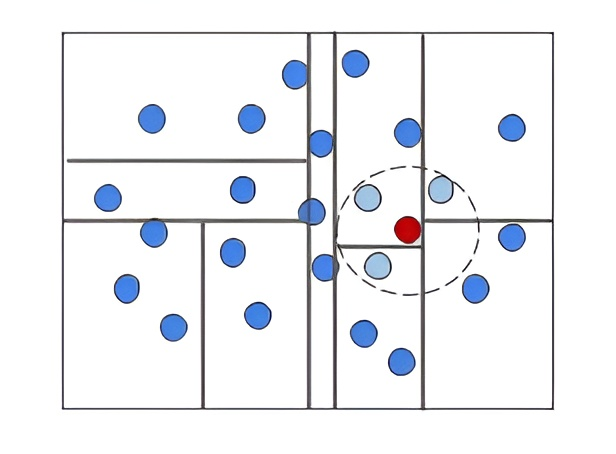
\includegraphics[width=0.5\columnwidth]{../img/related/treeb.jpg}
		\caption{Retrieval of 3-Nearest Neighbors (light blue) for a query vector (red) using a Tree-based index}        
		\label{fig:tree_retrieval}
\end{figure}

Tree-based methods for approximate similarity search have evolved to support both guaranteed and non-guaranteed searches (\textit{ng-approximate}). Exact methods use lower-bounding techniques to prune the search space without false negatives~\cite{conf/sigmod/Faloutsos1994}, whereas ng-approximate methods relax these guarantees to prioritize efficiency. For example, \textit{FLANN} constructs multiple randomized kd-trees and searches them in parallel, while \textit{HDIndex} segments the space into smaller regions, applying heuristics to speed up search~\cite{flann,hdindex}.

In ng-approximate search, tree-based methods often strike a balance between accuracy and efficiency by allowing users to specify parameters such as the number of leaves to visit or the search depth~\cite{hydra2,dumpy}. Some techniques apply dimensionality reduction before indexing~\cite{journal/kais/Camerra2014,journal/vldb/Zoumpatianos2016,dstree,ulisse,hercules}, while others index high-dimensional vectors directly~\cite{conf/vldb/Ciaccia1997}.

\noindent{\textbf{Hash-based Approaches:}} Hash-based methods, particularly those in the \textit{locality-sensitive hashing} (LSH) family~\cite{conf/stoc/indyk1998,lsh-survey}, are designed for \(\delta\)-\(\epsilon\)-approximate vector search. These methods use hash functions to map similar vectors into the same bucket with high probability, thus reducing the search space for high-dimensional vectors by clustering similar ones together.

\begin{figure}[ht] 
\centering
		\captionsetup{justification=centering}
		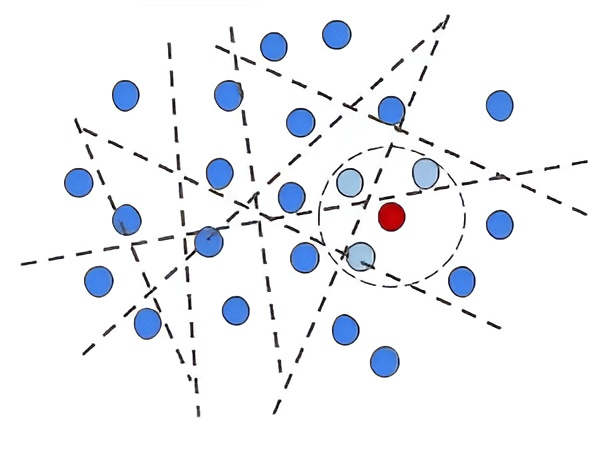
\includegraphics[width=0.5\columnwidth]{../img/related/hashb.jpg}
		\caption{Retrieval of 3-Nearest Neighbors (light blue) for a query vector (red) using Hash-based indexing}        
		\label{fig:hash_retrieval}
\end{figure}

Different variants of LSH have been proposed to optimize various aspects of search performance. \textit{Spherical Random Projection (SRS)}~\cite{srs} balances search efficiency with index size using random projections that maintain pairwise distances. \textit{Query-Aware Locality Sensitive Hashing (QALSH)}~\cite{qalsh} adjusts the hashing process to improve accuracy by incorporating the query vector into the hash function.

The trade-off between efficiency and accuracy in \(\delta\)-\(\epsilon\)-approximate searches can be fine-tuned by adjusting parameters such as the number of hash tables, the number of hash functions per table, and the number of random projections~\cite{qalsh,hydra2}. This flexibility makes hash-based methods an effective choice for fast search times with controllable approximation errors.

\noindent{\textbf{Graph-based Approaches:}} Graph-based methods support \textit{ng}-approximate vector search by organizing data into proximity graphs~\cite{gabriel69,toussaint02}. In such graphs, each vertex represents a data point, and edges are formed between vertices based on their proximity in the vector space, often determined by a distance measure like Euclidean distance~\cite{edelsbrunner87}. Graph traversal starts from a set of seed vertices, progressing in a best-first, greedy fashion until no better candidates are found~\cite{beamsearch}.

\begin{figure}[ht] 
\centering
		\captionsetup{justification=centering}
		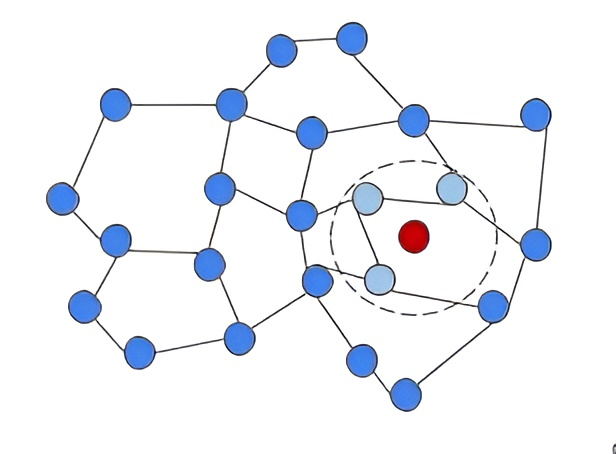
\includegraphics[width=0.5\columnwidth]{../img/related/graphb.jpg}
		\caption{Retrieval of 3-Nearest Neighbors (light blue) for a query vector (red) using Graph-based index structure}        
		\label{fig:graph_retrieval}
\end{figure}

State-of-the-art methods like \textit{KGraph}~\cite{kgraph}, \textit{HNSW}~\cite{hnsw}, \textit{NSG}~\cite{nsg}, \textit{Vamana}~\cite{vamana}, and \textit{ELPIS}~\cite{elpis} apply this general framework, but differ in how they construct the graph and choose initial entry points. These methods aim to strike a balance between connecting both short and long-range vertices while maintaining a sparse graph to minimize distance calculations, all while avoiding local minima.

The main challenge lies in managing this trade-off: too many edges complicate the routing process, while too few risk trapping the search in suboptimal regions of the graph. Modern graph-based methods focus on optimizing sparsity while maintaining robust connectivity, achieving high-speed, accurate search performance in large-scale vector datasets~\cite{hydra2,hnsw,nsg}.

\section{Summary of Approximate Search Methods}
\label{sec:summary_search_methods}

This section provides a summary of the key approximate similarity search methods, highlighting their primary strengths and weaknesses. Table~\ref{tab:methods_summary} presents an overview of the main characteristics, pros, and cons of each method.

\begin{table}[ht]
\centering
\begin{tabular}{|p{3cm}|p{4cm}|p{4cm}|p{4cm}|}
\hline
\textbf{Method} & \textbf{Description} & \textbf{Pros} & \textbf{Cons} \\ \hline
\textbf{Tree-based} & Organizes data in a hierarchical tree structure, enabling efficient pruning of the search space. & 
1. Low index construction time.
\newline 
2. Can support various search approaches.
& 
1. Lower search performance on difficult query workloads. \\ \hline

\textbf{Hash-based (LSH)} & Maps high-dimensional vectors into buckets using hash functions to group similar vectors. & 
1. Provides theoretical guarantees on query efficiency and accuracy. & 
1. Requires tuning multiple parameters (hash tables, hash functions). \newline 2. May reduce accuracy due to random hash assignments. \\ \hline

\textbf{Graph-based} & Constructs a proximity graph connecting vertices based on similarity, using greedy search to find neighbors. & 
1. Excellent empirical accuracy and efficiency.
& 
1. High index construction time and memory usage. \newline 2. Risk of getting stuck in local minima during search. \\ \hline
\end{tabular}
\caption{Summary of Approximate Search Methods: Pros and Cons}
\label{tab:methods_summary}
\end{table}

The major classes of approximate similarity search methods each present their own advantages and limitations. Tree-based methods provide hierarchical data organization, allowing for efficient pruning with relatively low index construction time, though they struggle with complex queries. Hash-based methods (LSH) group similar vectors into buckets, offering theoretical guarantees on performance, but require careful tuning and can suffer from reduced accuracy. Graph-based methods use proximity graphs to achieve high accuracy and efficient searching, but the high cost of building the index and the memory footprint are potential downsides.

\section{In-Memory vs Disk-Based Similarity Search}

Approximate similarity search algorithms can be broadly categorized into two approaches: \textit{in-memory} and \textit{disk-based} (or out-of-core). Both approaches aim to efficiently manage the retrieval of similar items from large-scale datasets but differ significantly in their handling of data storage and access.

\textbf{In-memory} approaches store all necessary data structures, such as proximity graphs or hash tables, in the main memory, enabling rapid access to data during query execution. These methods are highly efficient for query latency, as memory access times are orders of magnitude faster than disk operations. However, they are constrained by the machine's available memory, limiting their applicability to datasets that can fully reside within the main memory. In-memory methods are often the preferred choice for applications that require real-time or low-latency responses, such as recommendation systems or large-scale data retrieval tasks. Popular graph-based methods like HNSW~\cite{hnsw} and Vamana~\cite{vamana} have demonstrated excellent performance in in-memory settings but require significant memory resources during both graph construction and search.

\textbf{Disk-based} or \textit{out-of-core} approaches use the disk as an extension of the main memory, loading data segments into memory only as needed. This allows the algorithm to handle much larger datasets, often beyond the capacity of the machine’s RAM. Disk-based methods involve more complex data access patterns, which introduce significant I/O overhead, particularly when random disk accesses are required. To mitigate this, out-of-core algorithms often employ strategies that minimize random disk access by maximizing sequential I/O operations and improving data locality. For example, systems like DiskANN~\cite{vamana} and Hercules~\cite{hercules} provide disk-based solutions that can scale to extremely large datasets by efficiently managing memory and disk interactions, albeit at the cost of increased query latency.

Given the widespread use of large-scale datasets in modern similarity search applications, this thesis focuses on \textit{in-memory graph-based approaches}, which are particularly suitable for scenarios where fast query response times are critical, and the dataset can fit within available memory. While in-memory approaches offer significant advantages in terms of low latency and high query throughput, they are inherently limited by memory capacity, making them less practical for extremely large datasets that exceed memory limits. Nevertheless, for applications requiring high efficiency and manageable dataset sizes, in-memory graph-based methods strike a balance between query performance and accuracy. The following chapters will explore these techniques, presenting new optimizations aimed at improving their scalability and performance on large-scale data collections.

\section{Conclusion}

\noindent This chapter presented an overview of the main categories of approximate similarity search techniques, covering tree-based, hash-based, and graph-based methods. Each approach has distinct strengths and limitations in terms of performance, accuracy, and scalability, making them suitable for different scenarios and types of data. Tree-based methods are versatile, supporting multiple search strategies, but tend to underperform on complex or challenging workloads. Hash-based methods offer strong theoretical guarantees but require careful parameter tuning. In contrast, graph-based methods, though computationally more expensive to construct, have consistently shown superior empirical performance for large-scale datasets.

The following chapter will explore graph-based methods in greater detail, introducing a new taxonomy and key design paradigms that distinguish the various techniques. This will serve as a foundation for the development of novel methods aimed at further enhancing the efficiency of graph-based similarity search.

\graphicspath{{../img/graph/}}
\chapter{Graph-Based Approximate Vector Search}
\label{chapter:graphfamily}

\noindent Graph-based approaches have emerged as a leading solution for \textit{ng}-approximate similarity search due to their capability to effectively reduce the search space and provide low-latency, high-recall query results. In these methods, the dataset is organized as a proximity graph, where vertices represent data points, and edges connect similar vertices according to a specific distance metric. Through the use of beam search, these methods minimize the number of distance calculations, delivering near-optimal outcomes for approximate similarity search.

In this chapter, we offer a thorough review of existing in-memory graph-based techniques for \textit{ng}-approximate similarity search. We introduce a novel taxonomy that classifies these methods into five key paradigms: Seed Selection (SS), Neighborhood Propagation (NP), Incremental Insertion (II), Neighborhood Diversification (ND), and Divide-and-Conquer (DC). Additionally, we examine how critical components—such as seed selection strategies and edge pruning techniques—directly influence the graph's efficiency and performance. Through an evaluation of these design choices, we provide insights into how graph-based methods achieve superior performance across various datasets, laying the groundwork for the optimizations presented in the following chapters. 

\clearpage 
\section{Proximity Graphs and Beam Search}
\label{sec:proximity_graphs}

A \textbf{proximity graph} is formally defined as a graph \(G(\mathbb{V}, \mathbb{E})\), where \(\mathbb{V}\) represents the set of vertices (data points), and \(\mathbb{E}\) denotes the edges connecting pairs of vertices. Vertices \(V_i\) and \(V_j\) are connected if they satisfy a specific geometric condition, known as the \textit{neighborhood criterion}~\cite{shamos1975closest}. The most common distance metric employed is the Euclidean distance~\cite{edelsbrunner87}, although other measures such as the dot product~\cite{mipsg} may be used, depending on the dataset and the context.

One of the earliest proximity graphs is the \textit{Delaunay Graph (DG)}, which is the dual of the Voronoi Diagram~\cite{vd95}. In a DG, two vertices are connected if their Voronoi cells share an edge. Formally, for any three vertices \(q, p, r \in \mathbb{V}\), an edge exists between them in \(G(\mathbb{V}, \mathbb{E})\) if the circumcircle passing through \(q, p, r\) contains no other vertices from \(\mathbb{V}\)~\cite{aurenhammer2013voronoi}. While Delaunay graphs are efficient in low-dimensional spaces, they become nearly fully connected in high-dimensional datasets, leading to inefficiencies~\cite{dobkin1990delaunay}. To address this, modern proximity graphs adopt alternative structures that maintain a balance between graph sparsity and connectivity, improving scalability for large high-dimensional datasets~\cite{gabriel69, matula80, toussaint02}.

\subsection{Beam Search}
\label{subsec:beam_search}

\textbf{Beam search}, first introduced by Reddy in 1977~\cite{reddy77bm}, is a widely used algorithm in fields such as speech recognition, machine translation, and natural language processing. It enhances efficiency by exploring a limited subset of hypotheses, called the "beam," in contrast to exhaustive search methods. In proximity graphs, beam search iteratively traverses the graph starting from a set of seed vertices and explores their neighbors in a greedy, best-first manner. The process continues until the \(k\)-nearest neighbors of a query vector \(V_Q\) are found, or no better candidates are available~\cite{beamsearch}. Although beam search prioritizes speed over completeness and optimality~\cite{beamsearch, reddy77bm}, it remains effective for large-scale datasets, especially when low-latency query responses are critical.





The \textbf{time complexity} of beam search is determined by three factors: the beam width \(B\), the average outdegree \(m\), and the maximum path length \(T\) allowed within the graph, where \(T\) typically corresponds to the graph’s diameter in the worst case. The time complexity can be expressed as:

\begin{equation} \centering \text{Time Complexity} = O(B \times m \times T). \label{eq:time_complexity_beam_search} \end{equation}

where:
\begin{itemize}
   \item \( B \) represents the beam width,
   \item \( m \) denotes the average outdegree,
   \item \( T \) is the diameter of the graph.
\end{itemize}

Here, the beam width \(B\)  representing the number of hypotheses (candidates)  to keep in track during search; \(m\) is the average number of neighbors (branching factor); and \(T\) is the maximum allowed search path length, often equivalent to the graph's diameter~\cite{beamsearch}. Our empirical study of the theoretical complexity, presented in Appendix~\ref{appendix:beamsearch}, shows that the empirical complexity aligns with the theoretical complexity in most cases.

Although beam search is computationally efficient, search accuracy depends on the beam width, and determining the optimal width often requires experimentation. Additionally, the choice of \textit{seed selection} strategy can significantly affect performance, especially when retrieving a small number of nearest neighbors.


\begin{algorithm}[tb]
\small
\caption{Beam Search (G, $V_Q$, $s$, $k$, $L$)}\label{alg:beamsearch}
\begin{algorithmic}[1]
    \Require Graph $G$, query vector $V_Q$, initial seed $s$, result size $k$, beam width $L \geq k$
    \Ensure $k$ approximate nearest neighbors to $V_Q$
    \State Initialize candidate set $C \gets \{s\}$
    \State Initialize visited list $Visited \gets \emptyset$
    \While{$C \setminus Visited \neq \emptyset$}
        \State $p^{*} \gets \operatorname*{argmin}\limits_{V_i \in C \setminus R} \text{dist}(V_Q, V_i)$
        \State Update $Visited \gets Visited \cup \{p^{*}\}$
        \State Update $C \gets C \cup N_{\text{out}}(p^*)$        
        \If{$|C| > L$}
            \State Retain closest $L$ points in $C$ to $V_Q$
        \EndIf
    \EndWhile
    \State \Return The $k$ candidates in $C$ closest to $V_Q$
\end{algorithmic}
\end{algorithm}

The Beam Search leverages the structure of the proximity graph $G$ and the beam width \( L \) to efficiently navigate through the most relevant portions of the graph. For a given query vector $V_Q$ and starting from an initial seed node $s$, it maintains a candidate set $C$ and a visited list $Visited$. In each iteration, the algorithm selects the unvisited node $p^*$ from $C$ that is closest to $V_Q$, defined as $p^{*} \gets \operatorname*{argmin}\limits_{V_i \in C \setminus Visited} \text{dist}(V_Q, V_i)$. When adding the neighbors of $p^*$ to $C$, the algorithm checks for each neighbor whether it has not been visited and whether its distance to $V_Q$ is smaller than the $L$-th best-so-far (BSF) distance among the nodes in $C$. This selective expansion ensures that only promising candidates are considered, keeping the search focused and the candidate set size manageable.

Some versions of Beam Search introduce modifications such as adding a stopping criterion—terminating the search when the current node $p^*$ has a distance to $V_Q$ greater than the $L$-th BSF distance—and using two priority queues: one for nodes to visit and one for the results. In these variations, the result queue is limited to size $L$, while the queue for potential nodes to visit remains unbounded. However, our experiments indicate that these modifications are not practical. The stopping criterion can prematurely halt the search on challenging datasets, causing the algorithm to become trapped in local minima. Additionally, allowing an unbounded size for candidate nodes to visit is impractical, especially when the search starts from a region different from the actual nearest neighbors on a graph with high average outdegree. Some methods, such as HNSW, apply these modifications to Beam Search, but we show that using a single priority queue for all candidates without a stopping criterion is more efficient and helps the search reach better approximate answers on difficult datasets.



%The beam search leverages the structure of the proximity graph and the beam width \( L \) to efficiently navigate through the most relevant portions of the graph. By maintaining a limited set of candidate nodes and pruning based on the distance threshold \( d_L \), the algorithm reduces computational overhead while still providing high-quality approximate nearest neighbors. The early termination condition ensures that the search halts when further exploration is unlikely to yield better results, thus optimizing performance.


While beam search strikes a balance between efficiency and accuracy, it does not guarantee that the exact nearest neighbors will be found unless the beam width \(L\) is large enough to explore the entire search space. Nevertheless, with an appropriately tuned beam width, it can achieve near-exhaustive performance with much lower computational cost~\cite{beamsearch}.

Many state-of-the-art graph-based vector search methods, including HNSW~\cite{hnsw}, NSG~\cite{nsg}, ELPIS~\cite{elpis}, Vamana~\cite{vamana}, and NSSG~\cite{nssg}, adopt this beam search algorithm to retrieve ng-approximate neighbors. However, these methods primarily differ in how they construct the graph and initiate the beam search. The next section introduces a novel taxonomy of graph-based approximate vector search methods, highlighting five key design paradigms. We will also discuss the evolution of state-of-the-art techniques and evaluate critical design choices such as seed selection and neighborhood diversification.
\section{Main Paradigm}

\noindent{\bf{Seed Selection (SS)}} involves selecting the initial graph vertices to visit during query answering. It is also used during index construction by methods that utilize beam search to decide which edges to construct. Some approaches choose one or more seed(s) randomly, while others employ specialized data structures such as K-D Trees.

\noindent{\bf{NP-Based Methods}}: The neighborhood propagation (NP) approach refines a pre-existing graph, which could be random (as in KGraph~\cite{kgraph}), or based on alternative approximate search methods like tree-based Efanna~\cite{efanna} or hash-based IEH~\cite{ieh}. NP refines the neighborhood of each node by incorporating neighbors from its immediate neighbors, or from neighbors of neighbors, through a process called NNDescent~\cite{nndescent}. KGraph~\cite{kgraph} pioneered NP, influencing methods such as IEH~\cite{ieh}, EFANNA~\cite{efanna}, DPG~\cite{dpg}, NSG~\cite{nsg}, and NSSG~\cite{nssg}, which use NP-refined graphs as a base.

\noindent{\bf{Insertion-Based Methods}}: Methods such as NSW~\cite{nsw14}, HNSW~\cite{hnsw}, and ELPIS~\cite{elpis} construct graphs through sequential node insertion. This process draws from the VoroNet~\cite{voronet} overlay network, which was influenced by Kleinberg’s small-world model~\cite{kleinberg2000,kleinberg2002}. Each node connects to its nearest neighbors and long-range neighbors, facilitating efficient traversal. HNSW and ELPIS additionally prune neighbors using diversification strategies, categorizing them under both insertion-based and neighborhood diversification paradigms. Such methods are capable of handling large datasets~\cite{ann-benchmark-journal,elpis}.

\noindent{\bf{Neighborhood Diversification (ND)}}: Originally introduced by the Relative Neighborhood Graph (RNG)~\cite{rng}, ND aims to sparsify the graph by pruning redundant edges. The goal is to maintain efficient search connectivity by eliminating unnecessary connections, typically based on geometric properties of the graph. For each vertex \(X_q\), ND selectively retains neighbors \(X_i\) from a candidate set \(C_q\), optimizing graph sparsity while preserving proximity.

The principle of relatively close neighbors was introduced by Lankford in 1969~\cite{lankford69}. It defines two vertices \(V_i\) and \(V_j\) as relatively close if:

\begin{equation} \centering \text{dist}(V_i, V_j) \leq \max[\text{dist}(V_i, V_w), \text{dist}(V_w, V_j)] \quad \text{for all} \quad w \neq i,j. \label{eq:lankfordrng} \end{equation}
This principle has been adapted by various recent methods for approximate similarity search. ND creates long-range links by pruning close neighbors, allowing better graph traversal during search. We will further discuss ND approaches and their approximations in Section~\ref{sec:nd}.

\noindent{\bf{Divide-and-Conquer (DC)}}: The DC strategy partitions the dataset and constructs individual graphs for each partition. These graphs are later merged into a unified graph, or searched in parallel, as in SPTAG~\cite{SPTAG4} and HCNNG~\cite{hcnng}. ELPIS~\cite{elpis} maintains separate graphs for parallel search.

\noindent Among the paradigms, \textit{Seed Selection (SS)} and \textit{Neighborhood Diversification (ND)} exhibit the most variation in state-of-the-art methods. This thesis focuses on these paradigms, systematically evaluating their impact on performance across different datasets. The following sections provide in-depth analysis of SS and ND strategies.


\subsection{Seed Selection}
\label{sec:ss}
While state-of-the-art graph-based vector search methods adopt diverse strategies for constructing the graph, they virtually all use beam search for query answering (Algorithm~\ref{alg:beamsearch}).
The Beam Search initiated with a set of entry points \( s \) of size $ |s| \geq 1$, the algorithm maintains a candidate set \( C \) and a visited list \( R \), progressively exploring the graph by iteratively selecting the closest non-visited point to \( V_Q \) from \( C \), updating \( C \) with its neighbors, and marking it as visited. The beam width \( L \), ensuring a balance between accuracy and computational efficiency, limits the size of \( C \) at each step, focusing the search on the most promising candidates. The process continues until all candidates are visited, concluding with the return of the \( k \) points closest to \( V_Q \) from the candidate set. This approach ensures a guided and efficient traversal of the graph, making it a practical choice for graph-based ANNs task.
because it usually retrieves good answers if the graph is well-connected. However, choosing the right nodes to visit first has an impact on how quickly good answers are found. The longer the graph traversal, the higher the number of visited nodes, and the slower the search.
Several methods build one or more index(es), in addition to the graph, on top of a sample of data points. These additional indexes are used during query answering to find the entry points in the graph.
For instance, HNSW~\cite{hnsw} employs a hierarchical, multi-resolution NSW graphs, whereas SPTAG~\cite{SPTAG4}, EFANNA~\cite{efanna}, and HCNNG~\cite{hcnng} leverage multiple K-D Trees~\cite{kdtree} or BK-trees~\cite{bkmtree} to acquire initial seeds, and IEH~\cite{ieh} resorts to hash tables. In contrast, methods like DPG~\cite{dpg}, NSG~\cite{nsg}, Vamana~\cite{vamana}, and NSSG~\cite{nssg} argue that such an approach may not yield benefits in practice, opting instead for predefined representative points, such as the medoid of the graph (the node with the minimum sum of distances to others), or points randomly sampled before each search.

However, to the best of our knowledge, none of these methods have provided sufficient theoretical or empirical evidence to support their choices for seed selection. In this thesis, we conduct an in-depth study of the different seed selection techniques proposed in the literature:

\noindent (1) \textbf{Stacked-NSW (SN)}: Inspired by skip lists~\cite{skiplist}, HNSW~\cite{hnsw} constructs hierarchical multi-resolution graphs~\cite{nsw14} for seed selection. Each hierarchical layer consists of a Navigable Small World (NSW) graph, where each higher level samples nodes from the layer below, with the base layer containing the entire dataset. 

\begin{figure}[ht] 
\centering
		\captionsetup{justification=centering}
		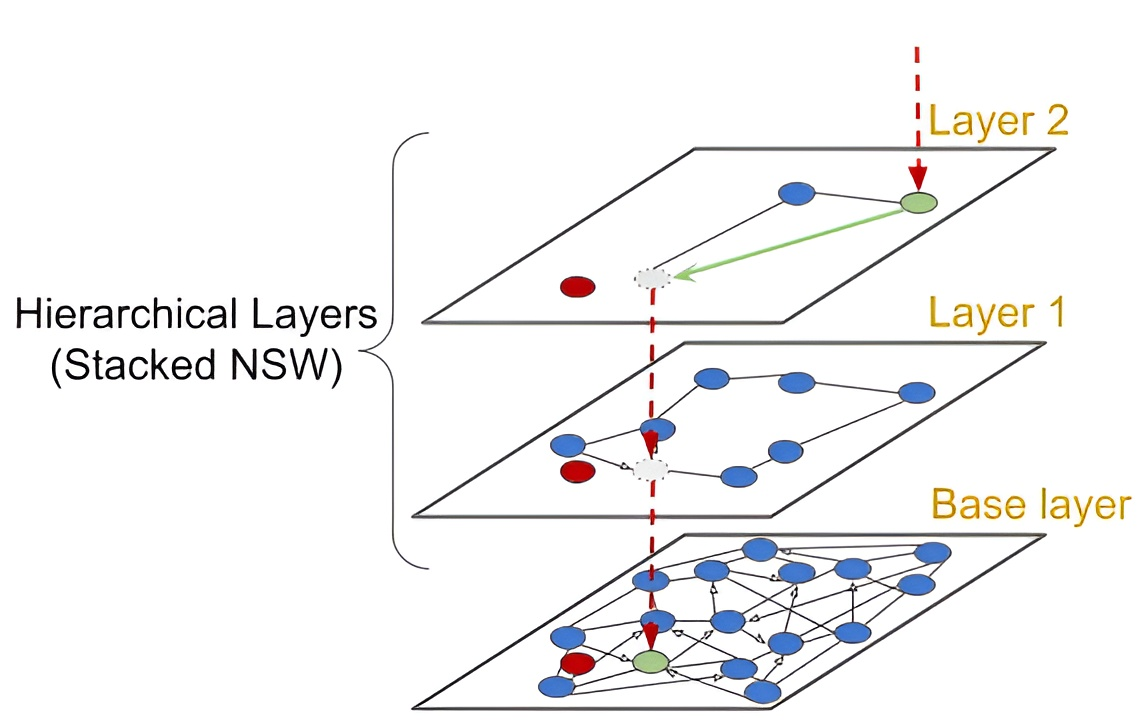
\includegraphics[width=0.7\columnwidth]{../img/graphfamily/snsw.png}
		\caption{Routing through SNSW during search on HNSW graph}        
		\label{fig:snwd}
 \end{figure}




The Stacked-NSW graph is constructed by assigning each node a maximum level L, which is generated using the formula:

\begin{equation} \centering L = \frac{-\ln(\xi)}{\ln\left(M/2\right)} \label{eq:1} \end{equation}

Where $\xi$ is a uniformly random number between 0 and 1, and MM is the maximum outdegree, which controls the probability distribution of a node's maximum layer. The logarithmic nature of the formula ensures that most nodes are concentrated in the lower layers, while only a few nodes reach the top layers.

As M increases, graph connectivity improves, concentrating nodes in the lower layers and reducing the number of hierarchical levels, which minimizes the number of distance calculations required for the beam search. Conversely, smaller values of MM shift more nodes to higher layers, enhancing seed quality for searches on sparse graphs. Table~\ref{tab:layer_distribution} illustrates the distribution of nodes across hierarchical layers for different MM values on the Deep1M dataset.

\begin{table}[ht]
\centering
\caption{Distribution of Nodes Across Hierarchical Layers Based on Outdegree \(M\)}
\label{tab:layer_distribution}
\resizebox{\textwidth}{!}{%
\begin{tabular}{|c|c|c|c|c|c|c|c|c|c|c|}
\hline
\textbf{M} & \textbf{Number of Layers} & \textbf{Layer 1} & \textbf{Layer 2} & \textbf{Layer 3} & \textbf{Layer 4} & \textbf{Layer 5} & \textbf{Layer 6} & \textbf{Layer 7} & \textbf{Layer 8} & \textbf{Layer 9} \\ \hline
5  & 9  & 200058 & 40583 & 7988  & 1581 & 304  & 76   & 11  & 3   & 1   \\ \hline
10 & 6  & 100636 & 10060 & 988   & 116  & 9    & 1    & 0   & 0   & 0   \\ \hline
15 & 5  & 67031  & 4438  & 292   & 18   & 1    & 0    & 0   & 0   & 0   \\ \hline
20 & 4  & 50487  & 2501  & 140   & 7    & 0    & 0    & 0   & 0   & 0   \\ \hline
\end{tabular}%
}
\end{table}

The hierarchical structure enables efficient search by constructing coarse neighborhoods at higher layers, allowing for long jumps in the search space. As the search progresses through lower layers, finer neighborhoods are formed, ultimately leading to the base layer, where the search continues within the most refined region. The search process begins at the highest layer and iteratively moves down through the layers, restarting the search at the next level upon reaching a local minimum, until the optimal entry point for beam search is found at layer 1.

\noindent (2) \textbf{K-D Trees (KD)}: Employed by EFANNA~\cite{efanna}, SPTAG-KDT~\cite{SPTAG2}, and HCNNG~\cite{hcnng}, this approach constructs one or multiple K-D Trees~\cite{kdtree} over a sample of the dataset. During query search, a depth-first search (DFS) traversal is conducted on the K-D Tree(s), providing a set of seed points to initialize the candidate list. The node closest to the query is selected as the entry point for further exploration.

\noindent (3) \textbf{Locality-Sensitive Hashing (LSH)}: Adopted by IEH~\cite{ieh}, LSH constructs a hash-based index on a sample of the dataset. During the search process, this index is used to generate a set of seed points, from which one is chosen as the entry node for the approximate nearest neighbor search.

\noindent (4) \textbf{Medoid (MD)}: Utilized by methods such as DPG~\cite{dpg}, NSG~\cite{nsg}, and Vamana~\cite{vamana}, this approach fixes the medoid node as the entry point during query search. The neighbors of the medoid are used as initial seeds, allowing for efficient exploration of the search space.

\noindent (5) \textbf{Single Fixed Random Entry Point (SF)}: In this strategy, a single random node is pre-selected and fixed as the entry point for all queries. The selected node and its neighbors are used as seed points for search, regardless of the query.

\noindent (6) \textbf{K-Sampled Random Seeds (KS)}: In each query, \(k\) random nodes are selected as seed points to initialize the search. This strategy is implemented in DPG~\cite{dpg}, NSG~\cite{nsg}, and Vamana~\cite{vamana}, where the medoid is combined with randomly chosen nodes to enhance the initial seed set.

\noindent (7) \textbf{Balanced K-means Trees (KM)}: Used by SPTAG-BKT~\cite{SPTAG2}, this method constructs Balanced K-means Trees (BKT)~\cite{bkmtree} over a sample of the dataset. During query search, a depth-first search (DFS) is performed on the BKT structure to retrieve seed points that warm up the candidate list.

In Section~\ref{sec:experiments_ND_SS}, We will compare most common approach for SS in literature, SN, KS, KD, on different datasets and sizes.




\subsection{Neighborhood Diversification}
\label{sec:nd}
In the initial stages of developing graph-based methods for similarity search, techniques such as KGraph proposed approximating the K-nearest neighbor (KNN) graph using NNDescent. This approach relies on iteratively propagating and updating neighborhood lists between connected vertices. Alternatively, NSW presented a graph construction method where nodes are incrementally inserted into the graph. During this process, each node’s neighborhood is retrieved via beam search, and bidirectional edges are established to connect the newly inserted node with those already in the graph. NSW particularly emphasized the importance of long-range edges to ensure efficient search. However, despite some differences in approach, both methods shared a common challenge: achieving good accuracy often required a large outdegree, leading to an increased number of distance calculations during the search.

Since then, several Neighborhood Diversification (ND) techniques have been developed to enhance graph-based data structures for similarity search. We classify graph-based approximate vector search methods that implement various ND strategies into a distinct ND-based class. The primary goal of ND is to create sparse graph structures by pruning unnecessary edges, while maintaining a well-connected network that ensures proximity between nodes. For a given node \( X_q \) and its list of candidate neighbors \( C_q \), the ND step strategically selects specific candidates \( X_i \) for inclusion in \( X_q \)’s neighborhood set \( R_q \). The core principle of ND is to diversify the selection of neighbors, improving the graph's efficiency during search traversal, while preserving the essential proximity relations within the structure.

The need for ND arises because searching a graph where nodes are only connected to their nearest neighbors may involve numerous redundant comparisons before reaching the optimal regions. The concept of ND was initially introduced with the Relative Neighborhood Graph (RNG)~\citep{rng,toussaint02}, which constructs an undirected graph either from scratch or by pruning an existing Delaunay Graph~\cite{dobkin1990delaunay}. In RNG, the longest edge in each triangle formed by three connected points is removed, which reduces redundant connections.

This idea, along with other geometrically motivated strategies, has since been adapted for directed graphs in several modern graph-based approximate similarity search methods~\citep{hnsw,dpg,nsg,nssg,vamana,SPTAG4,elpis}. We have identified three key ND strategies used in these methods: Relative Neighborhood Diversification (RND), Relaxed Relative Neighborhood Diversification (RRND), and Maximum-Oriented Neighborhood Diversification (MOND). 

It is worth noting that ND strategies differ from the small-world network model proposed by Kleinberg~\cite{kleinberg2000, kleinberg2002}, where long-range links are randomly chosen. In contrast, ND implicitly generates long-range links by pruning close neighbors, thus facilitating better traversal of the graph.

Below, we present formal definitions of each method, alongside relevant mathematical expressions and explanations of their operations. Figures~\ref{fig:ND:RND},~\ref{fig:ND:RRND}, and~\ref{fig:ND:MOND} illustrate how each method operates on a candidate neighborhood list.


\subsubsection{Relative Neighborhood Diversification (RND)}
RND was first introduced in the HNSW algorithm~\cite{hnsw} and has been used in other methods like NSG~\cite{nsg}, SPTAG~\cite{SPTAG4}, and ELPIS~\cite{elpis}. This method ensures that a candidate neighbor is added to the neighborhood of the query node only if it is closer to the query than to any already selected neighbors.

\begin{itemize}
    \item \(X_q\) is the query node, i.e., the node to be inserted into the graph.
    \item \(R_q\), the list of current closest neighbors to \(X_q\).
    \item \(C_q\), the list of candidate neighbors to \(X_q\) not yet in \(R_q\).
    \item \(X_j\) is a candidate neighbor being considered for inclusion in \(R_q\) and is part of \(C_q\).
    \item \(X_i\) is a node already in the set \(R_q\).
    \item \(\text{dist}(X_i, X_j)\) represents the Euclidean distance between nodes \(X_i\) and \(X_j\) in the \(d\)-dimensional space.
\end{itemize}

\begin{definition}
\label{def:rnd}
Given a query node \(X_q\), a candidate neighbor \(X_j\) is added to the list \(R_q\) if and only if:
\begin{equation}
    \forall X_i \in R_q, \, \text{dist}(X_q, X_j) < \text{dist}(X_i, X_j)
\end{equation}
\end{definition}

This ensures that redundant edges to nodes closer to each other than to the query node are pruned.

\begin{figure}[h]
    \centering
    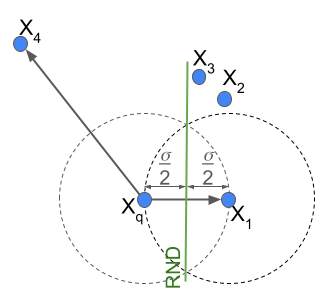
\includegraphics[width=0.4\textwidth]{../img/related/rnd.png}
    \caption{Example of RND pruning applied to the neighborhood list \(C_q\)}
    \label{fig:ND:RND}
\end{figure}

\subsubsection{Relaxed Relative Neighborhood Diversification (RRND)}
RRND, proposed by the Vamana algorithm~\cite{vamana}, relaxes the strict condition of RND by introducing a relaxation factor \(\alpha\). This factor allows nodes to be added to the neighborhood even if they do not strictly satisfy the RND condition, leading to a less aggressive pruning strategy and more neighbors retained.

\begin{itemize}
    \item \(X_q\) is the query node.
    \item \(R_q\), the list of current closest neighbors to \(X_q\).
    \item \(C_q\), the list of candidate neighbors to \(X_q\) not yet in \(R_q\).
    \item \(X_j\) is a candidate neighbor being considered for inclusion in \(R_q\) and is part of \(C_q\).
    \item \(X_i\) is a node already in the set \(R_q\).
    \item \(\alpha\) is the relaxation factor, where \(\alpha \geq 1\).
    \item \(\text{dist}(X_i, X_j)\) represents the Euclidean distance between nodes \(X_i\) and \(X_j\).
\end{itemize}

\begin{definition}
\label{def:rrnd}
Given a relaxation factor \(\alpha\), a candidate neighbor \(X_j\) is added to the list \(R_q\) if:
\begin{equation}
    \forall X_i \in R_q, \, \text{dist}(X_q, X_j) < \alpha \cdot \text{dist}(X_i, X_j)
\end{equation}
\end{definition}

When \(\alpha = 1\), RRND is reduced to RND. This relaxation increases graph connectivity by pruning fewer neighbors.

\begin{figure}[h]
    \centering
    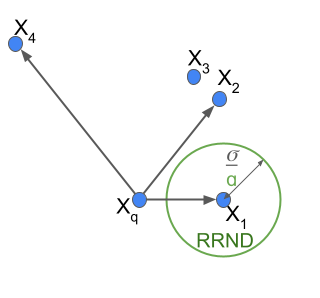
\includegraphics[width=0.4\textwidth]{../img/related/rrnd.png}
    \caption{Example of RRND pruning with relaxation factor \(\alpha = 1.5\)}
    \label{fig:ND:RRND}
\end{figure}

\subsubsection{Maximum-Oriented Neighborhood Diversification (MOND)}
MOND, introduced by DPG~\cite{dpg}, prunes candidate neighbors by focusing on the geometric orientation of edges, ensuring that neighbors are selected to maximize angular separation. This approach prevents the formation of cliques by ensuring that connections span diverse directions in the vector space.

\begin{itemize}
    \item \(X_q\) is the query node.
    \item \(R_q\), the list of current closest neighbors to \(X_q\).
    \item \(C_q\), the list of candidate neighbors to \(X_q\) not yet in \(R_q\).
    \item \(X_j\) is a candidate neighbor being considered for inclusion in \(R_q\) and is part of \(C_q\).
    \item \(X_i\) is a node already in the set \(R_q\).
    \item \(\theta\) is the angle threshold used to guide the pruning process.
    \item \(\angle X_j X_q X_i\) is the angle between the edges \(X_qX_j\) and \(X_qX_i\).
\end{itemize}

\begin{definition}
\label{def:mond}
Given an angle threshold \(\theta\), a candidate neighbor \(X_j\) is added to the list \(R_q\) if:
\begin{equation}
    \forall X_i \in R_q, \, \cos(\angle X_j X_q X_i) < \cos(\theta)
\end{equation}
\end{definition}

This strategy maximizes the angular separation of neighbors in the graph, leading to improved diversity in the neighborhood list.

\begin{figure}[h]
    \centering
    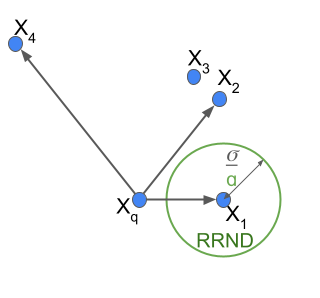
\includegraphics[width=0.4\textwidth]{../img/related/rrnd.png}
    \caption{Example of MOND pruning with angle threshold \(\theta = 60^\circ\)}
    \label{fig:ND:MOND}
\end{figure}

\subsection{Comparison of ND Methods}
As illustrated in Figures~\ref{fig:ND:RND},~\ref{fig:ND:RRND}, and~\ref{fig:ND:MOND}, these three methods vary in how they prune the candidate neighborhood set. RND applies the most stringent pruning criterion, whereas RRND loosens this condition using the relaxation factor \(\alpha\). On the other hand, MOND focuses on maximizing angular separation between neighbors to achieve diversification. These approaches have been demonstrated to enhance both the accuracy and efficiency of graph-based similarity search, with RND and MOND generally offering the optimal balance between computational cost and search accuracy~\cite{gass}.

Below, we prove that both MOND (Maximum-Oriented Neighborhood Diversification) and RRND (Relaxed Relative Neighborhood Diversification) are approximations of RND (Relative Neighborhood Diversification). Furthermore, we show that the converse does not hold, meaning RND does not necessarily approximate MOND or RRND.

\subsubsection{Preliminaries}

We define the necessary variables used in the proof as follows:

\begin{itemize}
    \item \(\mathbf{X}_q\) is the query node, i.e., the node to be inserted into the graph.
    \item \(\mathbf{R}_q\), the list of current closest neighbors to \(\mathbf{X}_q\).
    \item \(\mathbf{C}_q\), the list of candidate neighbors to \(\mathbf{X}_q\) not yet in \(\mathbf{R}_q\).
    \item \(\mathbf{X}_j\) is a candidate neighbor being considered for inclusion in \(\mathbf{R}_q\) and is part of \(\mathbf{C}_q\).
    \item \(\mathbf{X}_i\) is a node already in the set \(\mathbf{R}_q\).
    \item \(\text{dist}(\mathbf{X}_i, \mathbf{X}_j)\) represents the Euclidean distance between nodes \(\mathbf{X}_i\) and \(\mathbf{X}_j\) in the \(d\)-dimensional space.
\end{itemize}

\subsubsection{RRND as an Approximation of RND}

RRND introduces a relaxation factor \(\alpha \geq 1\) that allows edges to be retained even if they would be pruned under RND. The condition for RRND is:

\[
\forall \mathbf{X}_i \in \mathbf{R}_q, \; \text{dist}(\mathbf{X}_q, \mathbf{X}_j) < \alpha \cdot \text{dist}(\mathbf{X}_i, \mathbf{X}_j)
\]

Since \(\alpha \geq 1\), RRND retains more edges than RND. Specifically, if an edge is pruned by RRND, it will also be pruned by RND, but not necessarily the other way around, as RRND allows for more flexible edge retention. This establishes that RRND is an approximation of RND.

\subsubsection{MOND as an Approximation of RND}

MOND prunes edges based on angular separation. It retains neighbors that maximize the angular diversity in the graph. To show that MOND is an approximation of RND, we consider the following nodes:

\begin{itemize}
    \item \(\mathbf{X}_q\) is the query vector.
    \item \(\mathbf{X}_i\) is a neighbor already in \(\mathbf{R}_q\).
    \item \(\mathbf{X}_j\) is a candidate neighbor being considered for inclusion in \(\mathbf{R}_q\).
\end{itemize}

The condition for RND is:

\[
\forall \mathbf{X}_i \in \mathbf{R}_q, \; \text{dist}(\mathbf{X}_q, \mathbf{X}_j) < \text{dist}(\mathbf{X}_i, \mathbf{X}_j)
\]

MOND, however, adds \(\mathbf{X}_j\) to \(\mathbf{R}_q\) if the cosine of the angle between the edges \(\mathbf{X}_q \mathbf{X}_i\) and \(\mathbf{X}_q \mathbf{X}_j\) is less than a threshold \(\cos(\theta)\):

\[
\forall \mathbf{X}_i \in \mathbf{R}_q, \; \cos(\angle \mathbf{X}_i \mathbf{X}_q \mathbf{X}_j) < \cos(\theta)
\]

Where \(\theta\) is the angle threshold (e.g., \( \theta = 60^\circ \)).

\subsection{Proof that MOND Approximates RND}

In this section, we prove that MOND (Maximum-Oriented Neighborhood Diversification) is an approximation of RND (Relative Neighborhood Diversification). MOND aims to maximize the angular separation between edges in the neighborhood list, while RND prunes based on Euclidean distances. We show how the RND condition can be transformed into the angular condition used in MOND.

\subsubsection{Preliminaries}

We define the variables used in the proof:

\begin{itemize}
    \item \(\mathbf{X}_q\) is the query node, i.e., the node to be inserted into the graph.
    \item \(\mathbf{R}_q\) is the list of current closest neighbors to \(\mathbf{X}_q\).
    \item \(\mathbf{C}_q\) is the list of candidate neighbors to \(\mathbf{X}_q\) not yet in \(\mathbf{R}_q\).
    \item \(\mathbf{X}_j\) is a candidate neighbor being considered for inclusion in \(\mathbf{R}_q\).
    \item \(\mathbf{X}_i\) is a node already in the set \(\mathbf{R}_q\).
    \item \(\text{dist}(\mathbf{X}_i, \mathbf{X}_j)\) represents the Euclidean distance between nodes \(\mathbf{X}_i\) and \(\mathbf{X}_j\) in the \(d\)-dimensional space.
\end{itemize}

\subsubsection{RND Condition}

The RND condition states that a candidate neighbor \(\mathbf{X}_j\) is added to the neighborhood \(\mathbf{R}_q\) of \(\mathbf{X}_q\) if:

\[
\text{dist}(\mathbf{X}_q, \mathbf{X}_j) < \text{dist}(\mathbf{X}_i, \mathbf{X}_j), \quad \forall \mathbf{X}_i \in \mathbf{R}_q
\]

This condition ensures that \(\mathbf{X}_j\) is closer to the query node \(\mathbf{X}_q\) than to any existing neighbor \(\mathbf{X}_i\) in \(\mathbf{R}_q\).

\subsubsection{Transition to Angular Condition in MOND}

MOND, on the other hand, uses angular separation between neighbors to decide whether to add \(\mathbf{X}_j\) to \(\mathbf{R}_q\). Specifically, MOND retains \(\mathbf{X}_j\) if the cosine of the angle between the edges \(\mathbf{X}_q \mathbf{X}_i\) and \(\mathbf{X}_q \mathbf{X}_j\) is smaller than a threshold \(\cos(\theta)\), where \(\theta\) is the minimum required angular separation:

\[
\cos(\angle \mathbf{X}_i \mathbf{X}_q \mathbf{X}_j) < \cos(\theta)
\]

To prove that MOND approximates RND, we express the RND condition in terms of angles. Using the cosine law, the distance between two points can be related to the angle between the vectors. The cosine of the angle \(\angle \mathbf{X}_i \mathbf{X}_q \mathbf{X}_j\) can be written as:

\[
\cos(\angle \mathbf{X}_i \mathbf{X}_q \mathbf{X}_j) = \frac{\overrightarrow{\mathbf{X}_q \mathbf{X}_i} \cdot \overrightarrow{\mathbf{X}_q \mathbf{X}_j}}{|\overrightarrow{\mathbf{X}_q \mathbf{X}_i}| \cdot |\overrightarrow{\mathbf{X}_q \mathbf{X}_j}|}
\]

Now, using the Euclidean distances \(\text{dist}(\mathbf{X}_q, \mathbf{X}_i)\) and \(\text{dist}(\mathbf{X}_q, \mathbf{X}_j)\), the dot product of the vectors can be related to these distances. The RND condition implies:

\[
\text{dist}(\mathbf{X}_q, \mathbf{X}_j) < \text{dist}(\mathbf{X}_i, \mathbf{X}_j)
\]

This translates to:

\[
|\overrightarrow{\mathbf{X}_q \mathbf{X}_j}| < |\overrightarrow{\mathbf{X}_i \mathbf{X}_j}|
\]

Therefore, if the distance between \(\mathbf{X}_q\) and \(\mathbf{X}_j\) is small enough, the angle \(\angle \mathbf{X}_i \mathbf{X}_q \mathbf{X}_j\) will be large, ensuring that MOND will retain \(\mathbf{X}_j\) under the angular condition:

\[
\cos(\angle \mathbf{X}_i \mathbf{X}_q \mathbf{X}_j) < \cos(\theta)
\]

Thus, if \(\mathbf{X}_j\) is added by RND, it will also satisfy the angular condition of MOND, proving that MOND is an approximation of RND.

\subsubsection{Counter-Example: RND Does Not Approximate MOND}

To demonstrate that RND does not necessarily approximate MOND, we consider a simple 2D example where:

\[
\mathbf{X}_q = (0, 0), \quad \mathbf{X}_i = (2, 0), \quad \mathbf{X}_j = (1.8, 2.5)
\]

First, calculate the distances:

\[
\text{dist}(\mathbf{X}_q, \mathbf{X}_i) = \sqrt{(2 - 0)^2 + (0 - 0)^2} = 2
\]

\[
\text{dist}(\mathbf{X}_q, \mathbf{X}_j) = \sqrt{(1.8 - 0)^2 + (2.5 - 0)^2} = \sqrt{3.24 + 6.25} \approx 3.08
\]

Since \(\text{dist}(\mathbf{X}_q, \mathbf{X}_j) > \text{dist}(\mathbf{X}_q, \mathbf{X}_i)\), RND would prune \(\mathbf{X}_j\). Now, calculate the angle for MOND:

\[
\overrightarrow{\mathbf{X}_q \mathbf{X}_i} = (2, 0), \quad \overrightarrow{\mathbf{X}_q \mathbf{X}_j} = (1.8, 2.5)
\]

\[
\overrightarrow{\mathbf{X}_q \mathbf{X}_i} \cdot \overrightarrow{\mathbf{X}_q \mathbf{X}_j} = 2 \cdot 1.8 + 0 \cdot 2.5 = 3.6
\]

\[
|\overrightarrow{\mathbf{X}_q \mathbf{X}_i}| = 2, \quad |\overrightarrow{\mathbf{X}_q \mathbf{X}_j}| \approx 3.08
\]

\[
\cos(\theta) = \frac{3.6}{2 \times 3.08} \approx 0.586
\]

Since \( \cos(60^\circ) = 0.5 \), MOND will retain \(\mathbf{X}_j\), but RND would have pruned it. Therefore, MOND approximates RND, but RND does not always approximate MOND.



\subsubsection{Counter-Example: RND Does Not Approximate MOND}

To demonstrate that RND does not necessarily approximate MOND, consider a case in 2D where:

\[
\mathbf{X}_q = (0, 0), \quad \mathbf{X}_i = (2, 0), \quad \mathbf{X}_j = (1.8, 2.5)
\]

First, calculate the distances:

\[
\text{dist}(\mathbf{X}_q, \mathbf{X}_i) = \sqrt{(2 - 0)^2 + (0 - 0)^2} = 2
\]

\[
\text{dist}(\mathbf{X}_q, \mathbf{X}_j) = \sqrt{(1.8 - 0)^2 + (2.5 - 0)^2} = \sqrt{3.24 + 6.25} \approx 3.08
\]

Since \(\text{dist}(\mathbf{X}_q, \mathbf{X}_j) > \text{dist}(\mathbf{X}_q, \mathbf{X}_i)\), RND will prune \(\mathbf{X}_j\). Now, calculate the angle for MOND:

\[
\overrightarrow{\mathbf{X}_q \mathbf{X}_i} = (2, 0), \quad \overrightarrow{\mathbf{X}_q \mathbf{X}_j} = (1.8, 2.5)
\]

\[
\overrightarrow{\mathbf{X}_q \mathbf{X}_i} \cdot \overrightarrow{\mathbf{X}_q \mathbf{X}_j} = 2 \cdot 1.8 + 0 \cdot 2.5 = 3.6
\]

\[
|\overrightarrow{\mathbf{X}_q \mathbf{X}_i}| = 2, \quad |\overrightarrow{\mathbf{X}_q \mathbf{X}_j}| \approx 3.08
\]

\[
\cos(\theta) = \frac{3.6}{2 \times 3.08} \approx 0.586
\]

Since \( \cos(60^\circ) = 0.5 \), MOND will not prune \(\mathbf{X}_j\), but RND would have pruned it. Hence, MOND is not fully approximated by RND.




 




\section{Taxonomy of State-of-the-Art Graph-Based Approaches for Approximate Vector Search}

Figure~\ref{fig:roadmap} illustrates the classification of state-of-the-art graph-based methods, categorized into five fundamental design paradigms: Seed Selection (SS), Neighborhood Propagation (NP), Incremental Insertion (II), Neighborhood Diversification (ND), and the Divide-and-Conquer (DC) strategy.

\begin{figure}[ht] 
\centering
		\captionsetup{justification=centering}
		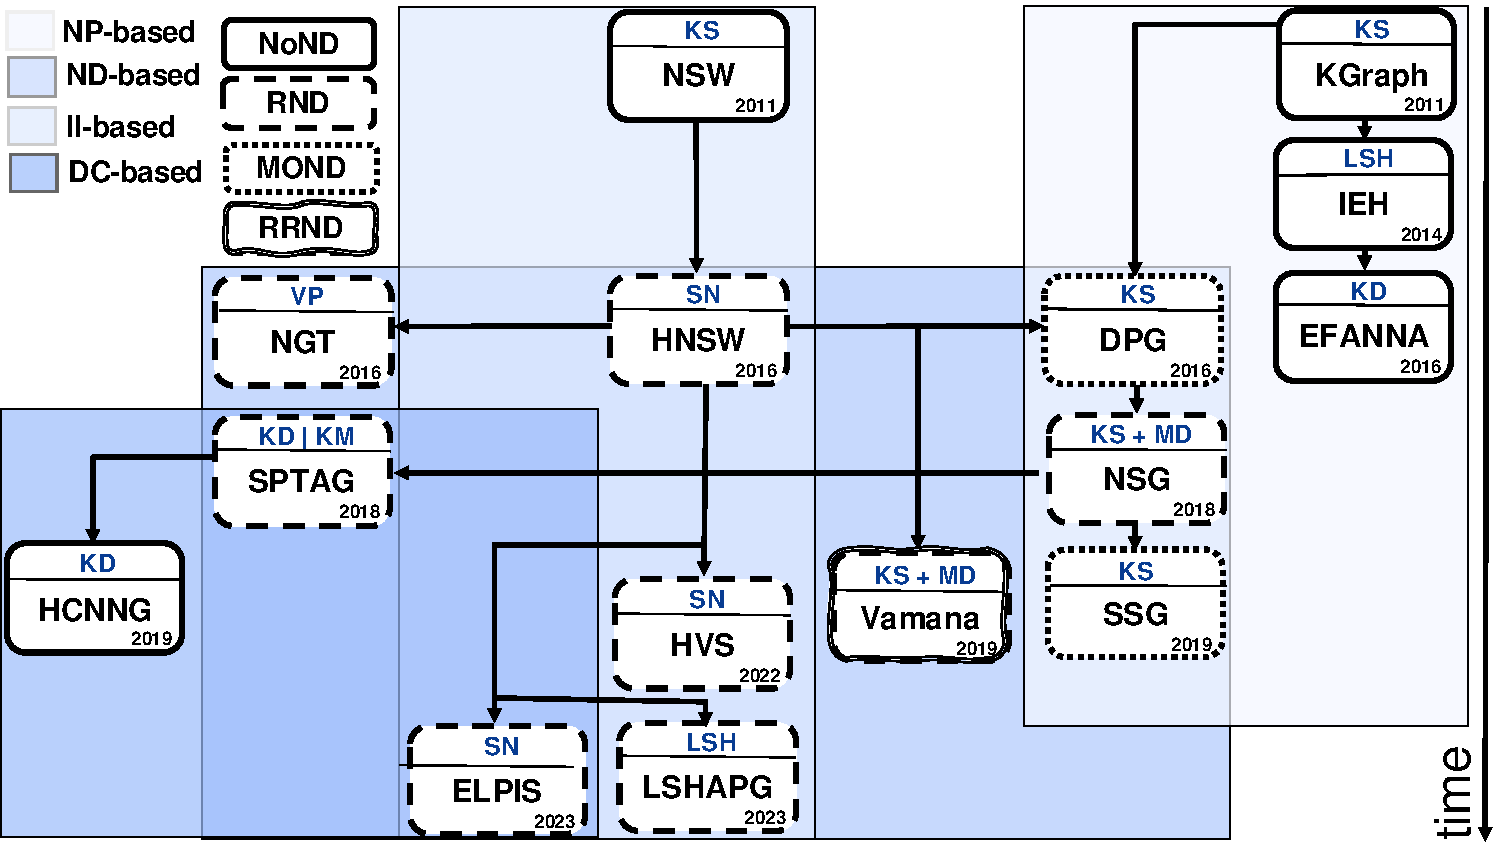
\includegraphics[width=\columnwidth]{../img/graphfamily/RoadMAPGANNS.pdf}
		\caption{Graph-Based Approximate Indexing Paradigms}        
		\label{fig:roadmap}
\end{figure}
The taxonomy further illustrates the evolution of these methods over time, with directed arrows showing how certain approaches have influenced others. Within the ND category, different strategies are highlighted, including No Neighborhood Diversification (NoND), RND, RRND, and MOND. Each method's Seed Selection (SS) strategy is also represented, such as KS, KD, SN, MD, LSH, and KM. (SF is proposed in this work but has not yet been adopted by existing methods.) Some methods incorporate multiple strategies, as seen in NSG and VAMANA, which leverage both KS and MD, or SPTAG, which alternates between KD and KM. Notably, many methods can integrate more than one paradigm. For example, HNSW combines Incremental Insertion (II) with neighborhood pruning using RND, thus falling into both II and ND categories.
KGraph~\cite{kgraph} was the first approach to employ NP for approximating the exact k-NN graph (k-NNG), which has quadratic complexity, and it subsequently influenced several methods like IEH~\cite{ieh} and EFANNA~\cite{efanna}. Concurrently, NSW~\cite{nsw11} introduced the II strategy for graph construction, which was later refined by HNSW~\cite{hnsw} and DPG~\cite{dpg} through the integration of ND to enhance the performance of NSW and KGraph, respectively.

The effectiveness of HNSW and DPG motivated other methods to adopt ND, such as NSG~\cite{nsg} and SSG~\cite{nssg}, which applied ND on the NP-based graph created by EFANNA~\cite{efanna}. SPTAG~\cite{SPTAG4} combined the DC paradigm with ND, while Vamana~\cite{vamana} followed NSG’s lead by constructing the graph via beam search, applying both RRND and RND in two rounds of pruning. HCNNG~\cite{hcnng}, inspired by SPTAG, incorporated a DC approach without employing ND. Similarly, ELPIS~\cite{elpis}, while using DC, leveraged both II and ND.

Earlier methods, with the exception of NSW, predominantly relied on NP. However, more recent efforts have shifted towards leveraging the ND, II, and DC paradigms due to their superior performance~\cite{aumuller2017ann, shimomura2021survey, graph-survey-vldb}, which will be further illustrated in Chapter~\ref{sec:experiments}.

In the next section, we will review the state-of-the-art techniques for in-memory graph-based approximate vector search.

\subsection{State-of-the-Art Approaches} 

\noindent{\bf KGraph}~\cite{kgraph} reduces the construction complexity of an exact k-NNG, which is quadratic in the worst case. It constructs an approximate k-NNG by refining a randomly initialized graph with an empirical time complexity of \( O(n^{1.14}) \)~\cite{nndescent}. This refinement process, referred to as NNDescent~\cite{nndescent} (Neighborhood Propagation), improves the approximation of the \( k \)-NN graph based on the assumption that a vertex's neighbors are more likely to be neighbors of each other. The process iterates over all vertices in the graph, and for each vertex \( u \), it considers every pair \( (x,y) \) of its neighbors. It adds \( x \) to the neighbors of \( y \) and vice versa, retaining only the closest \( k \) neighbors for each vertex.

\noindent{\bf Iterative Expanding Hashing (IEH)}~\cite{ieh} follows a similar process to KGraph in building an approximate k-NNG but generates initial candidates for each node using a hashing function. Two extensions of IEH, IEH-LSH~\cite{iehlsh} and IEH-ITQ~\cite{iehitq}, were proposed to improve the effectiveness of the initial candidates through more advanced hashing techniques. All these methods refine the graph using NNDescent~\cite{nndescent}.

\noindent{\bf EFANNA}~\cite{efanna} adopts seed selection and candidate refinement similar to KGraph~\cite{kgraph} and IEH~\cite{ieh}. It builds an approximate k-NNG by initially selecting the neighbors of each vertex through randomized truncated K-D Trees~\cite{dasgupta2008random}, and then applies NNDescent~\cite{nndescent} to refine the graph. During search, EFANNA utilizes these pre-built trees to retrieve initial seeds and then performs beam search on the graph index.

\noindent{\bf Navigable Small World (NSW)}~\cite{nsw11,nsw14} approximates a Delaunay graph that guarantees the small-world property~\cite{watts98}, where the number of hops \(L\) between two randomly chosen vertices grows logarithmically with the graph size \(n\), i.e., \(L \propto \log(n)\). NSW is derived from the VoroNet graph~\cite{voronet}, an extension of Kleinberg's small-world model~\cite{kleinberg2000,kleinberg2002}. The VoroNet graph is incrementally built by inserting randomly selected vertices and connecting them to \(2d+1\) neighbors chosen through beam search on the existing vertices. The early edges act as long-range connections, facilitating rapid traversal~\cite{voronet}, and the resulting graph ensures small-world properties~\cite{voronet,beaumont07}.

\noindent{\bf Hierarchical Navigable Small World (HNSW)}~\cite{hnsw} addresses the scalability limitations of NSW~\cite{nsw11,nsw14} by proposing the use of RND for neighborhood pruning and a multi-hierarchical seed selection strategy (SN). Each hierarchical layer contains a subgraph of the layer beneath it, with the base layer covering the entire dataset \( \mathbb{S} \). HNSW incrementally builds an NSW graph but refines candidate neighbors in each layer using RND. During query search, HNSW leverages SN to quickly locate an entry point in the base layer, from which beam search is initiated.

\noindent{\bf Diversified Proximity Graph (DPG)}~\cite{dpg} extends KGraph~\cite{kgraph} by introducing a diversification technique known as Maximum-Oriented Neighborhood Diversification (MOND), which maximizes the angles between neighbors to create a sparser graph. MOND is applied iteratively to all nodes, and the directed graph is then converted into an undirected graph for improved connectivity. Despite MOND being the focus, DPG's public implementation~\cite{dpgrepo} actually employs RND for neighborhood diversification instead of MOND.

\noindent{\bf Navigating Spreading-out Graph (NSG)}~\cite{nsg} also builds an approximate k-NNG but constructs an EFANNA graph instead of a KGraph. NSG diversifies its graph using RND and constructs a depth-first search (DFS) tree to ensure the graph's connectivity. Any disconnected vertices are linked to their nearest connected vertex to maintain overall graph structure.

\noindent{\bf Vamana}~\cite{vamana} follows a similar approach to NSG, utilizing visited nodes to build long-range edges. However, Vamana begins by creating a random graph with node degrees \( \geq \log(n) \) to ensure initial graph connectivity~\cite{erconnect}. A beam search is performed for each node, and the visited nodes are refined using RRND. Bi-directional edges are added, and the neighborhood list is further pruned using RND. The process is repeated to enhance graph quality, applying RRND in the second round to increase graph connectivity.

\noindent{\bf SSG}~\cite{nssg} integrates the MOND strategy from DPG~\cite{dpg} and mirrors the construction methods of NSG~\cite{nsg} and DPG~\cite{dpg}. Rather than searching each node for candidates, SSG uses breadth-first search (BFS) to gather candidate neighbors through local expansion on a base graph (EFANNA). When the maximum candidate list size is reached, SSG applies MOND to prune neighbors forming small angles (below a threshold \( \theta \)) with existing neighbors. Multiple DFS trees are built from different random points to enhance connectivity, compared to NSG's single DFS tree.

\noindent{\bf NGT}~\cite{ngt_library} is an approximate nearest neighbor (ANN) search library developed by Yahoo Japan. It offers two construction methods: one extends KNN graphs with reverse edges, forming bi-directed KNN graphs~\cite{ngtpanng1}, while the other incrementally builds graphs similar to HNSW with a range-based search strategy~\cite{ngtpanng2}.  In this study, we consider the former~\cite{ngtpanng1}. Additionally, the library includes methods that employ quantization for highly efficient search.
NGT maintains efficiency by pruning neighbors via RND and using Vantage-Point Trees~\cite{vptree} to select seed nodes for accurate query results

\noindent{\bf SPTAG}~\cite{SPTAG4}, developed by Microsoft, follows a divide-and-conquer (DC) approach. SPTAG selects small dataset samples and builds K-D Trees~\cite{kdtree} or Balanced K-means Trees~\cite{bkmtree}, which are used for seed selection. The full dataset is clustered using TP Trees~\cite{tptree}, and exact k-NN graphs are built and refined using ND for each cluster. The graphs are merged to form a single large graph for query processing.

\noindent{\bf Hierarchical Clustering-based Nearest Neighbor Graph (HCNNG)}~\cite{hcnng}, inspired by SPTAG, uses hierarchical clustering to divide the dataset into overlapping subsets. Each subset forms a Minimum Spanning Tree (MST), and the vertices and edges from all MSTs are merged to construct a unified graph. To aid search, HCNNG builds multiple K-D Trees~\cite{kdtree} to identify initial entry points during query processing.

\noindent{\bf HVS}~\cite{hvs} extends HNSW's base layer by refining the construction of hierarchical layers. Instead of random selection, nodes are assigned to layers based on local density to better capture data distribution. Each layer forms a Voronoi diagram, with nodes representing Voronoi cells, 
and uses multi-level quantization, increasing dimensionality by a factor of 2 in each lower layer.
%\(2^i\) at each lower layer, and i is the number of the layer. 
Search at the base layer is similar to that of HNSW.
%, ensuring accurate nearest neighbor retrieval while maintaining efficiency across layers.

\noindent{\bf LSHAPG}~\cite{lshapg} combines HNSW graphs with multiple hash tables based on the LSB-Tree structure~\cite{lsb} to enhance search efficiency. It leverages $L$ hash tables to retrieve seeds for beam search on the base layer, unlike HNSW, which selects a single seed through SN. LSHAPG also utilizes these hash tables for probabilistic routing during search, pruning neighbors based on the projected distance %between its projection and the query’s projection 
before evaluating and pruning the raw vectors.
%to reduces the computational cost of neighbor pruning during beam search.


\noindent{\bf ELPIS}~\cite{elpis}, our proposed approach for approximate vector search, employs a divide-and-conquer strategy. ELPIS partitions the dataset into multiple subsets using the Hercules EAPCA tree~\cite{hercules}, with each leaf corresponding to a different subset. A graph-based index is then constructed in parallel for each leaf using HNSW~\cite{hnsw}. During search, ELPIS heuristically selects an initial cluster via DFS traversal of the EAPCA tree and initiates beam search on the corresponding graph.

In the following chapter, we provide a detailed explanation of ELPIS and present a comparative analysis of state-of-the-art methods across various datasets and scales. Additionally, the next section will focus on experiments examining different approaches to seed selection and neighborhood diversification, along with a theoretical and empirical analysis of beam search complexity across graph-based methods.

\section{Experimental Evaluation}
\label{sec:experiments_ND_SS}

In this section, we present an evaluation of the various seed selection and neighborhood diversification methods. To isolate the effects of each strategy, we first implement a basic Incremental Insertion (II) method, where nodes are inserted incrementally. Each node \(i\) obtains its list of candidate neighbors through a beam search on the current partial graph containing the previously inserted nodes. Subsequently, we apply each strategy individually to the resulting graph.

We conduct tests using both real-world and synthetic datasets: (i) \emph{Deep}~\cite{url/data/deep1b}, which contains 1 billion vectors of 96 dimensions extracted from the final layers of a convolutional neural network; (ii) \emph{Sift}~\cite{conf/icassp/jegou2011,url/data/sift}, consisting of 1 billion 128-dimensional SIFT vectors representing image features; and (iii) synthetic datasets generated randomly, comprising RandPow0, RandPow5, and RandPow50, each with 256 dimensions, generated according to a power law distribution~\cite{powerlaw} using exponents of 0 (uniform~\cite{url/power-law}), 5, and 50 (highly skewed distributions). Power law distributions, expressed as \(Y = kX^a\), model many real-world phenomena (e.g., in economics, biology, social networks). The skewness of the distribution increases with \(a\), where \(a = 0\) represents a uniform distribution.

We experiment with subsets of various sizes from the real datasets, referring to each by its name and size in gigabytes (e.g., Deep25GB). For the largest datasets, we use the 1M and 1B prefixes to refer to 1-million and 1-billion vector subsets, respectively.

The query sets contain 100 individual vectors, processed one at a time to simulate real-world query scenarios where queries arrive unpredictably~\cite{itsawreport,DBLP:conf/edbt/GogolouTPB19,conf/sigmod/gogolou20}. In cases where results are reported for 1 million queries, these are extrapolated from the 100-query sets. For Deep and Sift, queries are randomly sampled from the available query workloads.

We measure the number of \textit{distance calculations} required to answer each query. Additionally, we assess the accuracy of each \(k\)-NN query using \textit{Recall}, which reflects the proportion of true nearest neighbors that the query \(S_Q\) successfully retrieves.

\subsection{Neighborhood Diversification}
\label{subsec:experiments-ND}

We now assess the performance of the neighborhood diversification (ND) strategies introduced in Section~\ref{sec:nd}, namely RND, RRND, and MOND, compared against a baseline with no neighborhood diversification (NoND). Each strategy is applied independently to an II-based graph, where nodes are inserted sequentially, and each node is connected to a pruned list of neighbors. The list is determined through beam search with a maximum outdegree of \(R = 60\) and a beam width of \(L = 800\). Bi-directional edges are created between neighbors, and the neighborhood list is pruned down to \(R\) neighbors using the corresponding ND strategy.

Graphs are built on the Deep and Sift datasets with sizes of 25GB, 100GB, and 1B. For RRND and MOND, we test various values of \(\alpha\) (ranging from 1 to 2) and \(\theta\) (ranging from \(50^\circ\) to \(80^\circ\)), respectively. The values \(\alpha = 1.3\) and \(\theta = 60^\circ\) are used in the final experiments, as they yield the best results. Each workload consists of 100 queries, and we evaluate the trade-off between accuracy and efficiency by measuring recall and the number of distance calculations performed during search.

\noindent{\textbf{Pruning Ratio.}} In the previous section, we demonstrated that RND applies more aggressive pruning compared to RRND, which relaxes the pruning condition using the parameter \(\alpha\), and MOND, as established through our theoretical proofs. Our theoretical findings align with the empirical pruning ratios of the three methods, as depicted in Figure \ref{fig:pruning_ratio}. The figure illustrates the average pruning ratio across nodes during graph construction for the Deep and Sift 25GB datasets:

\begin{figure}[h]
    \centering
    \captionsetup{justification=centering}
    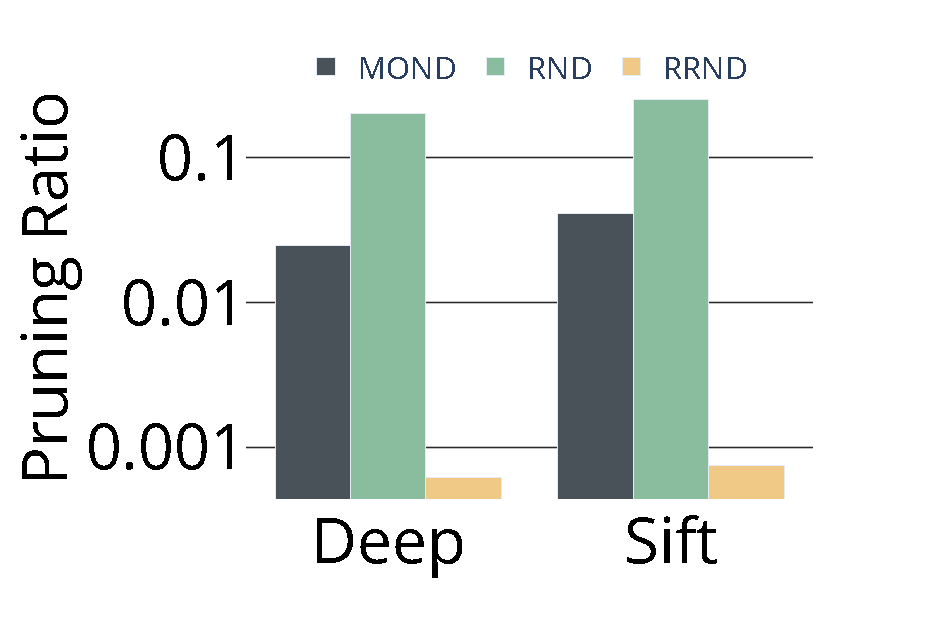
\includegraphics[width=0.5\textwidth]{../img/Experiments/RNG/pruningratio_n.pdf}
    \caption{Average pruning ratio across nodes during graph building for 25GB datasets.}
    \label{fig:pruning_ratio}
\end{figure}

During graph construction using incremental insertion, the pruning ratio is calculated for each node based on the KNN results obtained by performing a beam search on the partial graph of already inserted nodes. This candidate neighbors list is then pruned based on the neighborhood diversification method. The pruning ratio is defined as the ratio of the candidate neighbors list size before and after the pruning process. A lower value indicates less pruning, while a higher value signifies more aggressive pruning.

In both the Deep and Sift datasets, our empirical results show that RND achieves the highest pruning ratio, with 20\% and 25\% respectively. MOND comes second with 2\% and 4\%, while RRND, with a default value of \(\alpha = 1.5\), prunes the least, at 0.6\% and 0.7\%, respectively, in the Deep and Sift datasets.

\noindent{\textbf{Comparison of Query Performance on Real-world Datasets.}}
Figure~\ref{fig:ND:search:real} shows that both RND and MOND consistently outperform RRND, while NoND performs the worst across all datasets. As the dataset size increases, the performance gap between NoND and the ND-based methods widens, especially at high recall levels (Figures \ref{fig:ND:sift1b} and \ref{fig:ND:deep1b}). This is due to the increased number of hops required to find nearest neighbors and the dense neighborhoods formed in the NoND method, where no pruning is applied.

These results emphasize the critical role of the ND paradigm in enhancing query-answering performance, with RND and MOND emerging as the most effective strategies.

\begin{figure}[h!]
	\captionsetup{justification=centering}
	\centering	
		\begin{subfigure}{\columnwidth}
			\centering
			\captionsetup{justification=centering}	
			
\includegraphics[width=0.4\columnwidth]{../img/Experiments/RNG/legend.png}
			\label{fig:ND:legend}
		\end{subfigure}\\
		\begin{subfigure}{0.28\columnwidth}
			\centering
			\captionsetup{justification=centering}	
			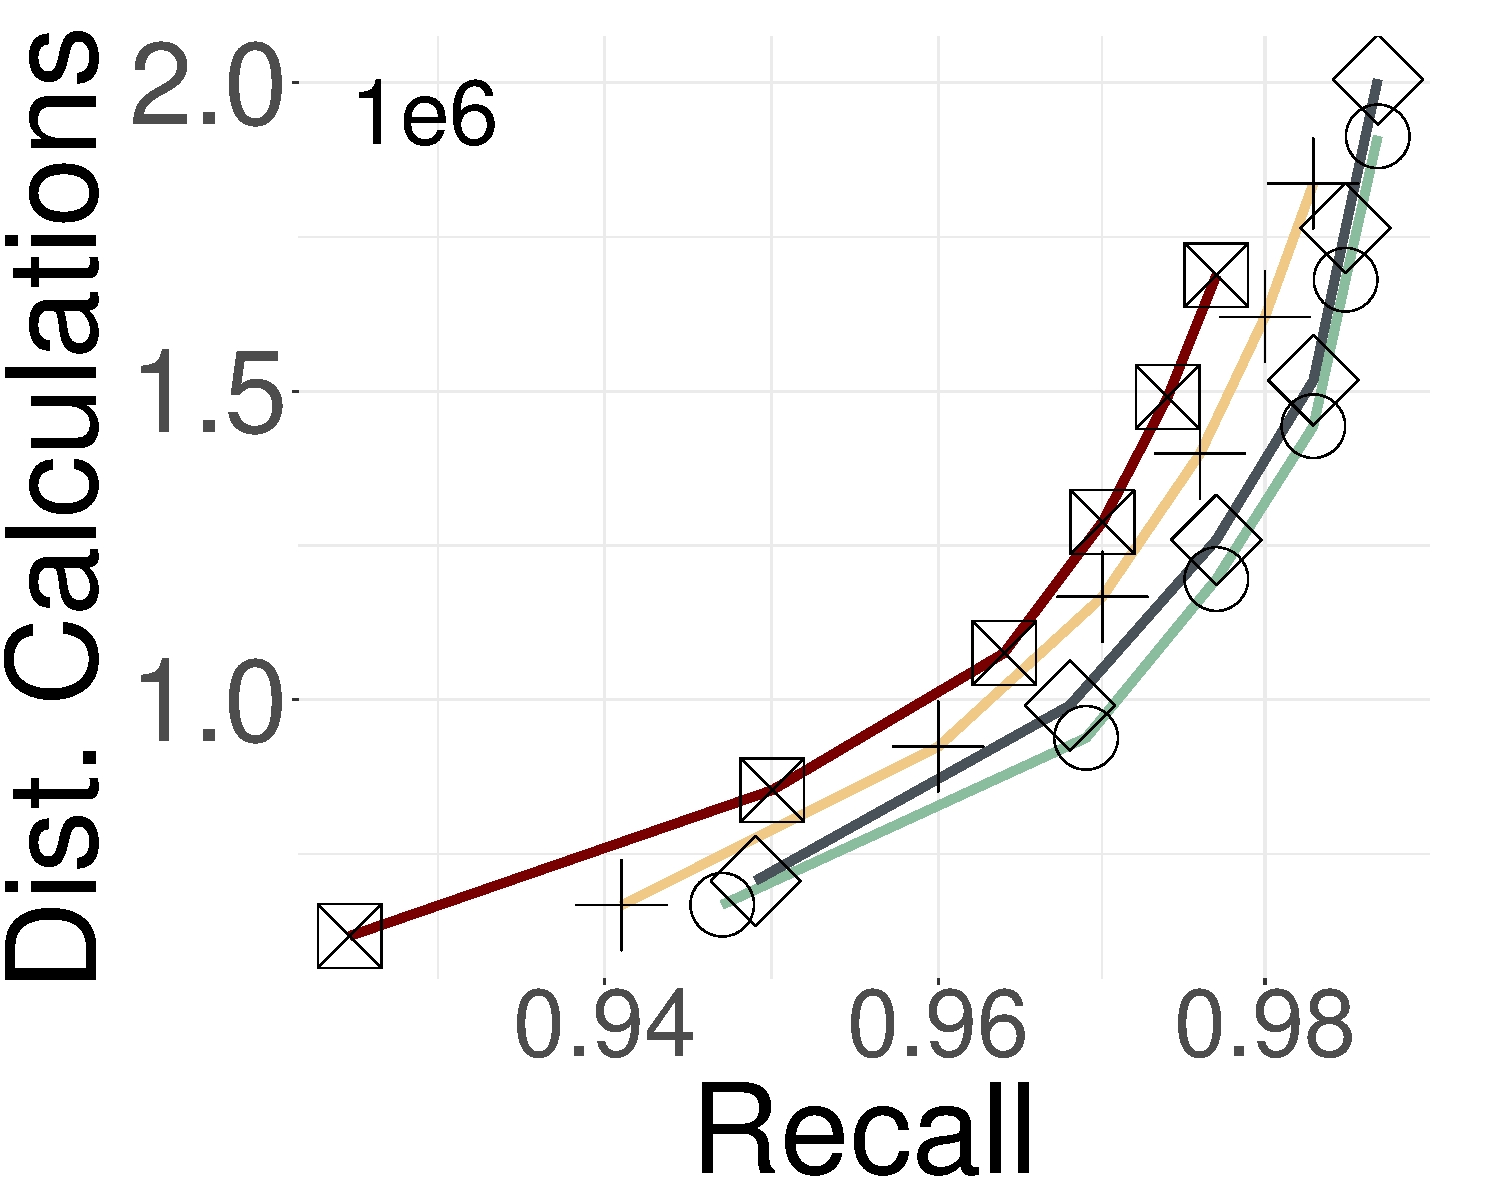
\includegraphics[width=\textwidth]{../img/Experiments/RNG/DC_DEEP25GB.pdf}
		\caption{{DEEP25GB}}
		\label{fig:ND:deep25GB}	
		\end{subfigure}	
  \hspace{0.5cm}
		\begin{subfigure}{0.28\columnwidth}
			\centering
			\captionsetup{justification=centering}	
			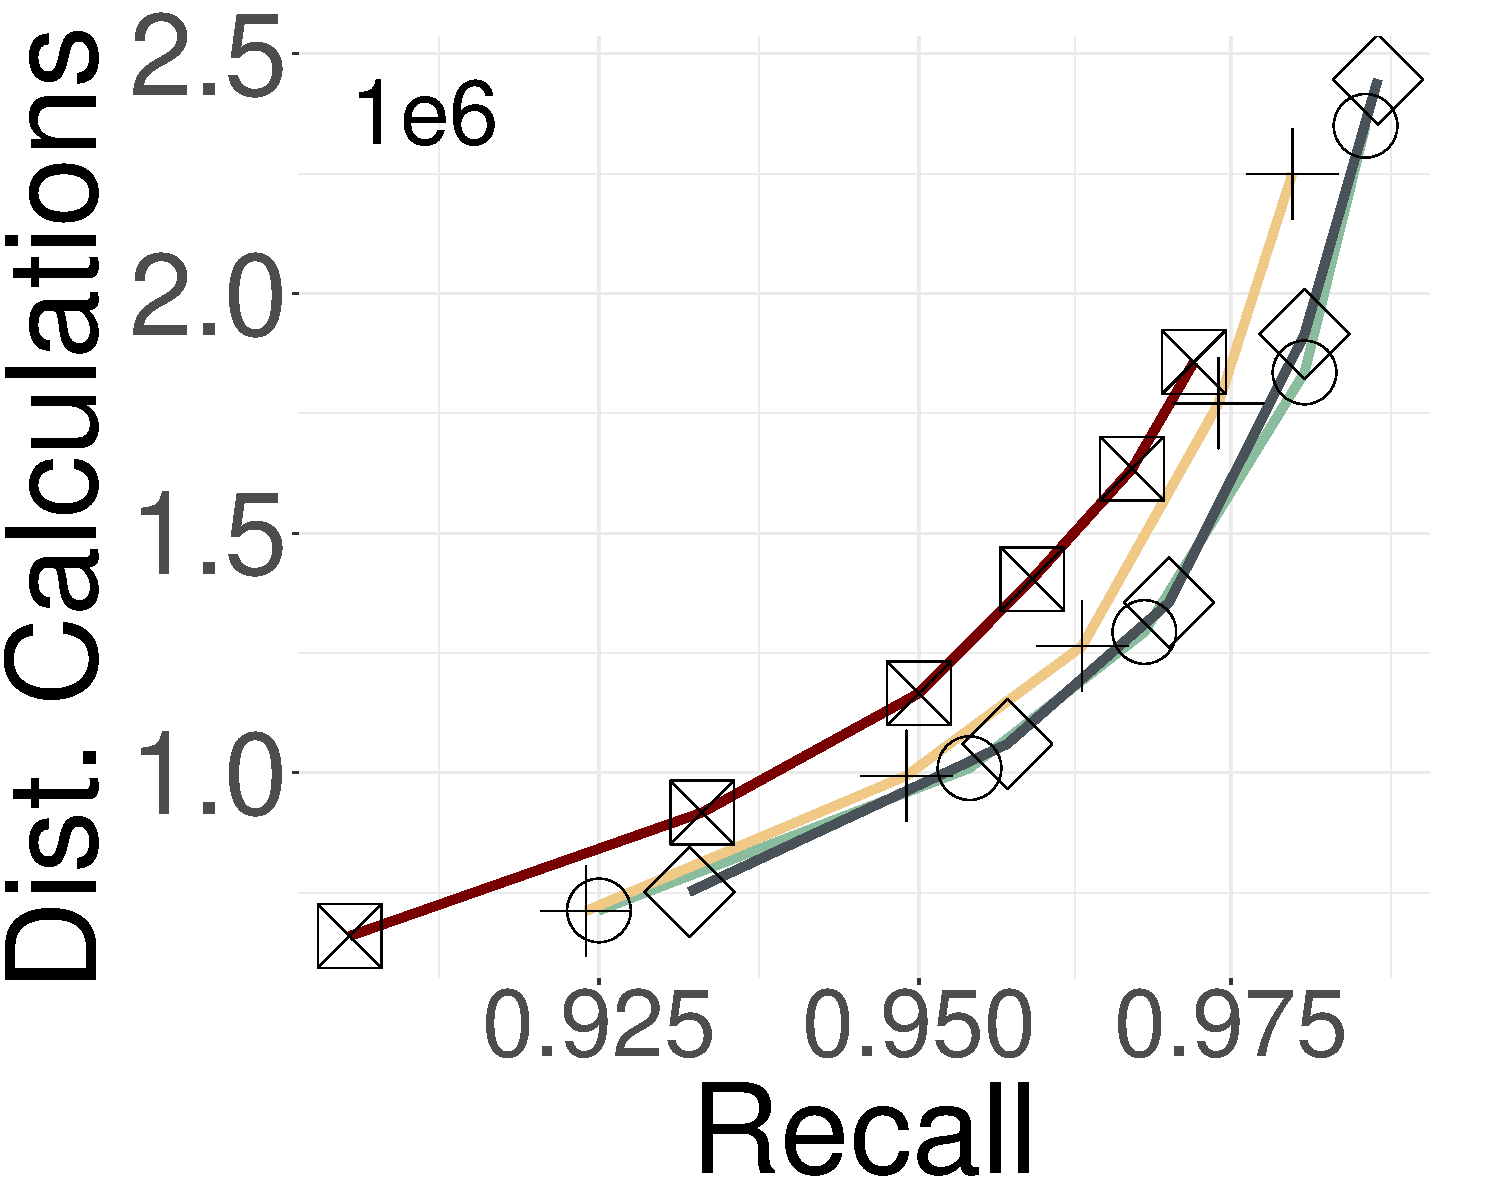
\includegraphics[width=\textwidth]{../img/Experiments/RNG/DC_DEEP100GB.pdf}
		\caption{{DEEP100GB}}
		\label{fig:ND:deep100GB}
		\end{subfigure}	
  \hspace{0.5cm}
		\begin{subfigure}{0.28\columnwidth}
			\centering
			\captionsetup{justification=centering}	
			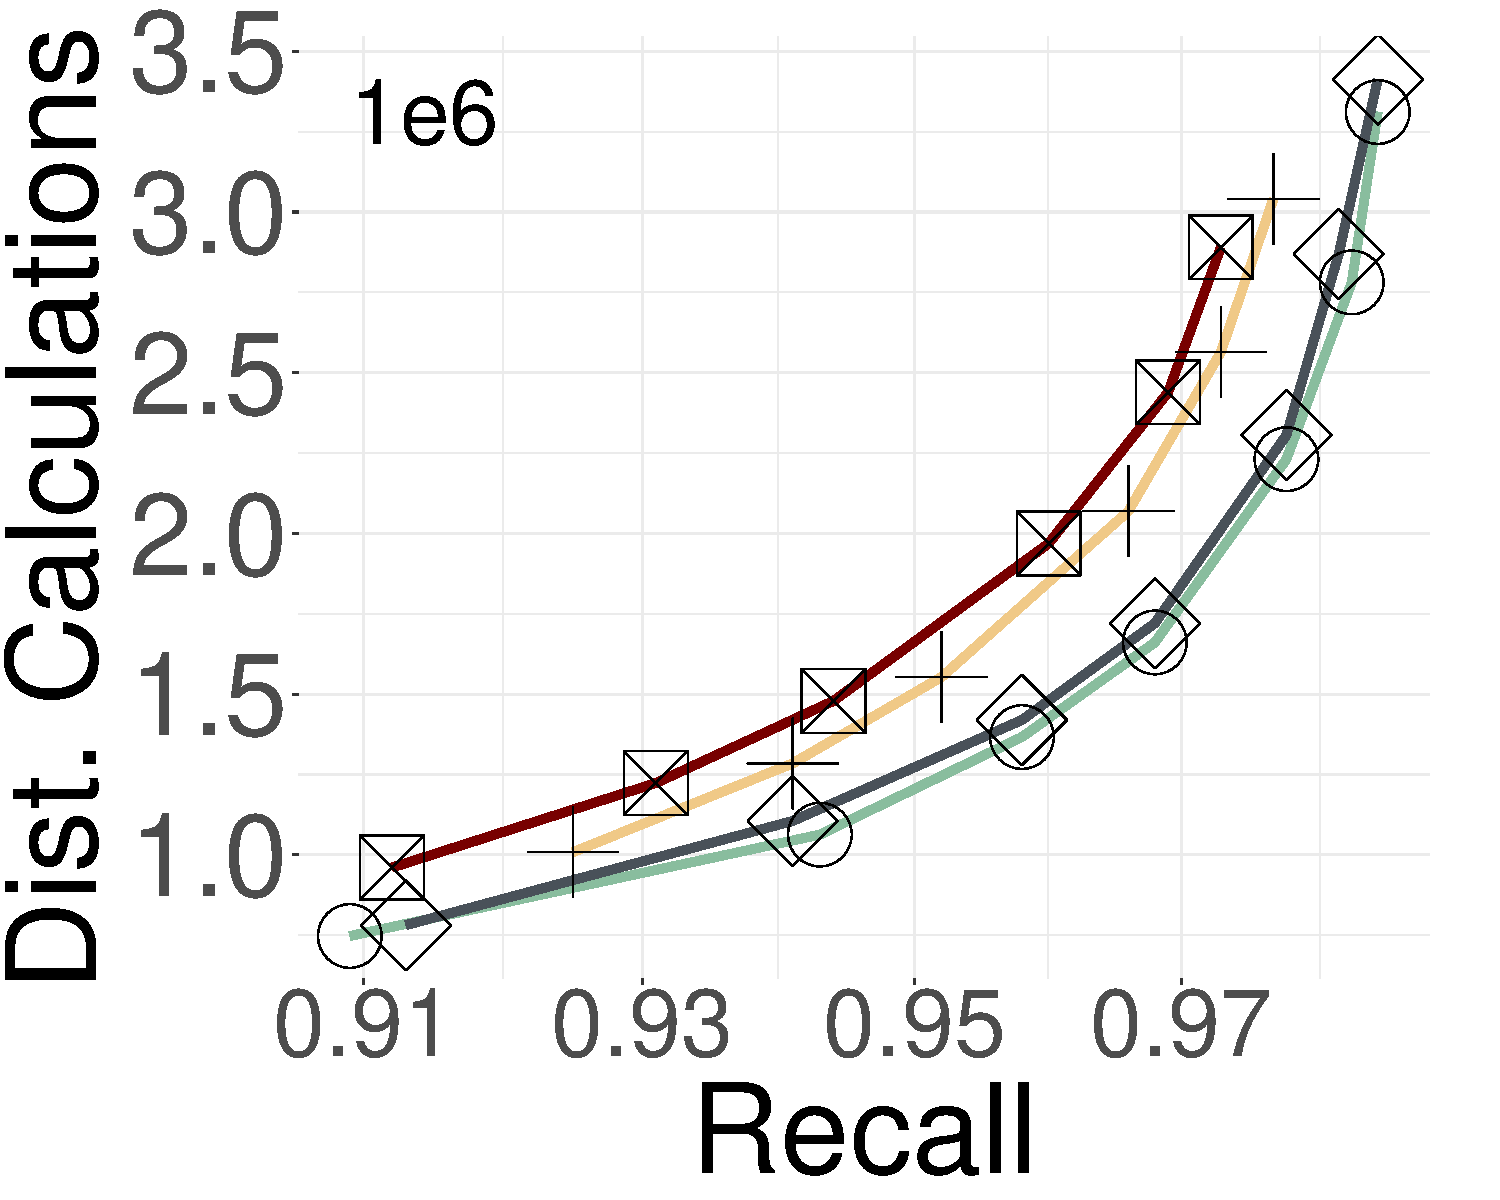
\includegraphics[width=\textwidth]{../img/Experiments/RNG/DC_DEEP1B.pdf}
		\caption{{DEEP1B}}%need to be updated
		\label{fig:ND:deep1b}	
  \end{subfigure}	
 
		\begin{subfigure}{0.28\columnwidth}
			\centering
			\captionsetup{justification=centering}	
			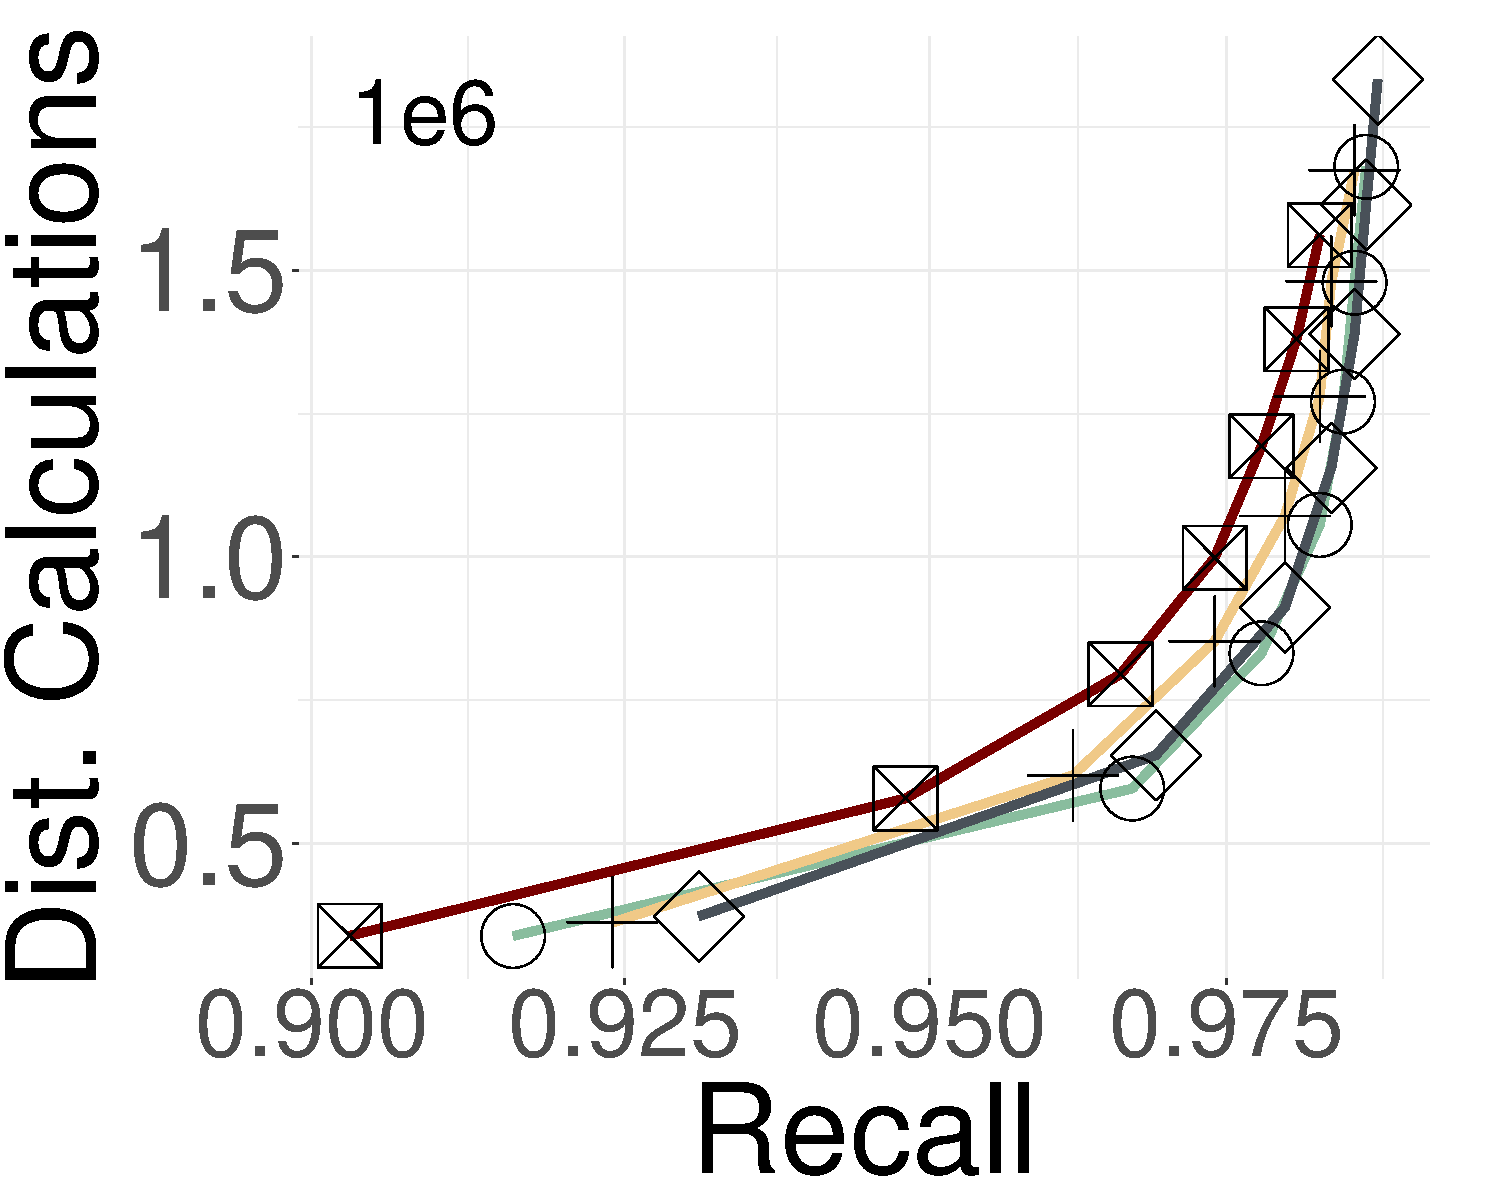
\includegraphics[width=\textwidth]{../img/Experiments/RNG/DC_SIFT25GB.pdf}
   \caption{{SIFT25GB}}
		\label{fig:ND:sift25GB}
		\end{subfigure}	
  \hspace{0.5cm}
		\begin{subfigure}{0.28\columnwidth}
			\centering
			\captionsetup{justification=centering}	
			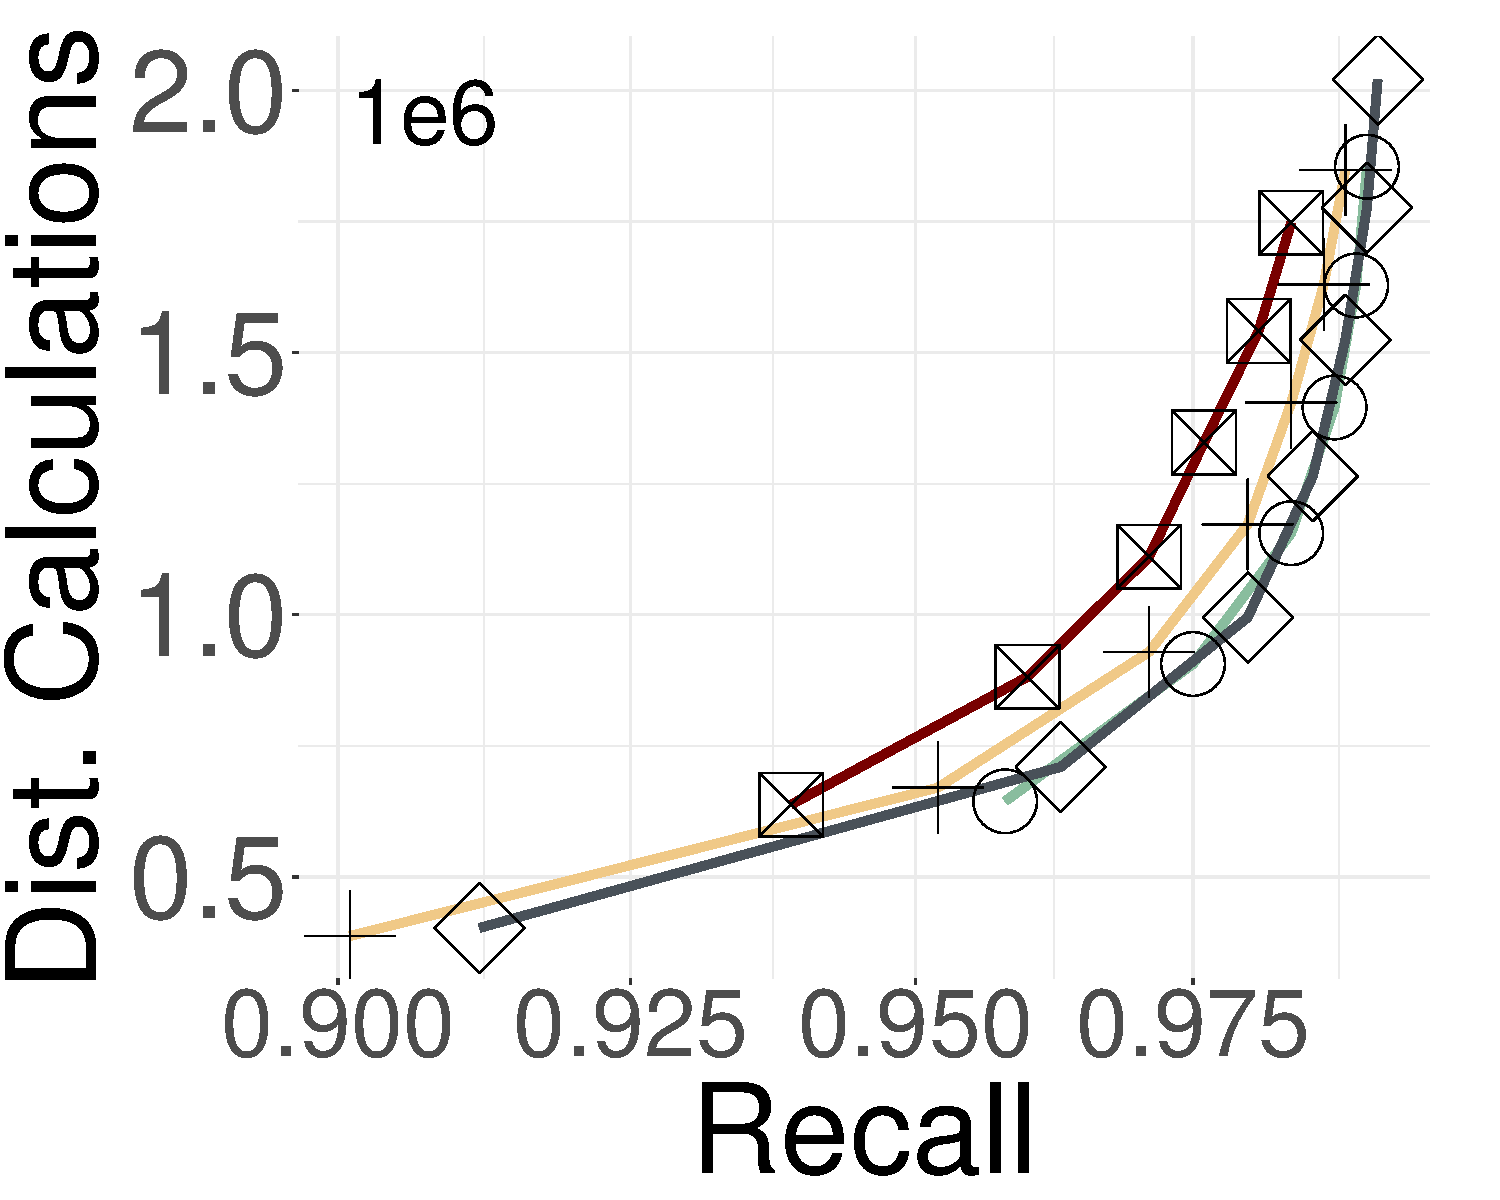
\includegraphics[width=\textwidth]{../img/Experiments/RNG/DC_SIFT100GB.pdf}
             \caption{{SIFT100GB}}
		      \label{fig:ND:sift100GB}
		\end{subfigure}	
  \hspace{0.5cm}
		\begin{subfigure}{0.28\columnwidth}
			\centering
			\captionsetup{justification=centering}	
			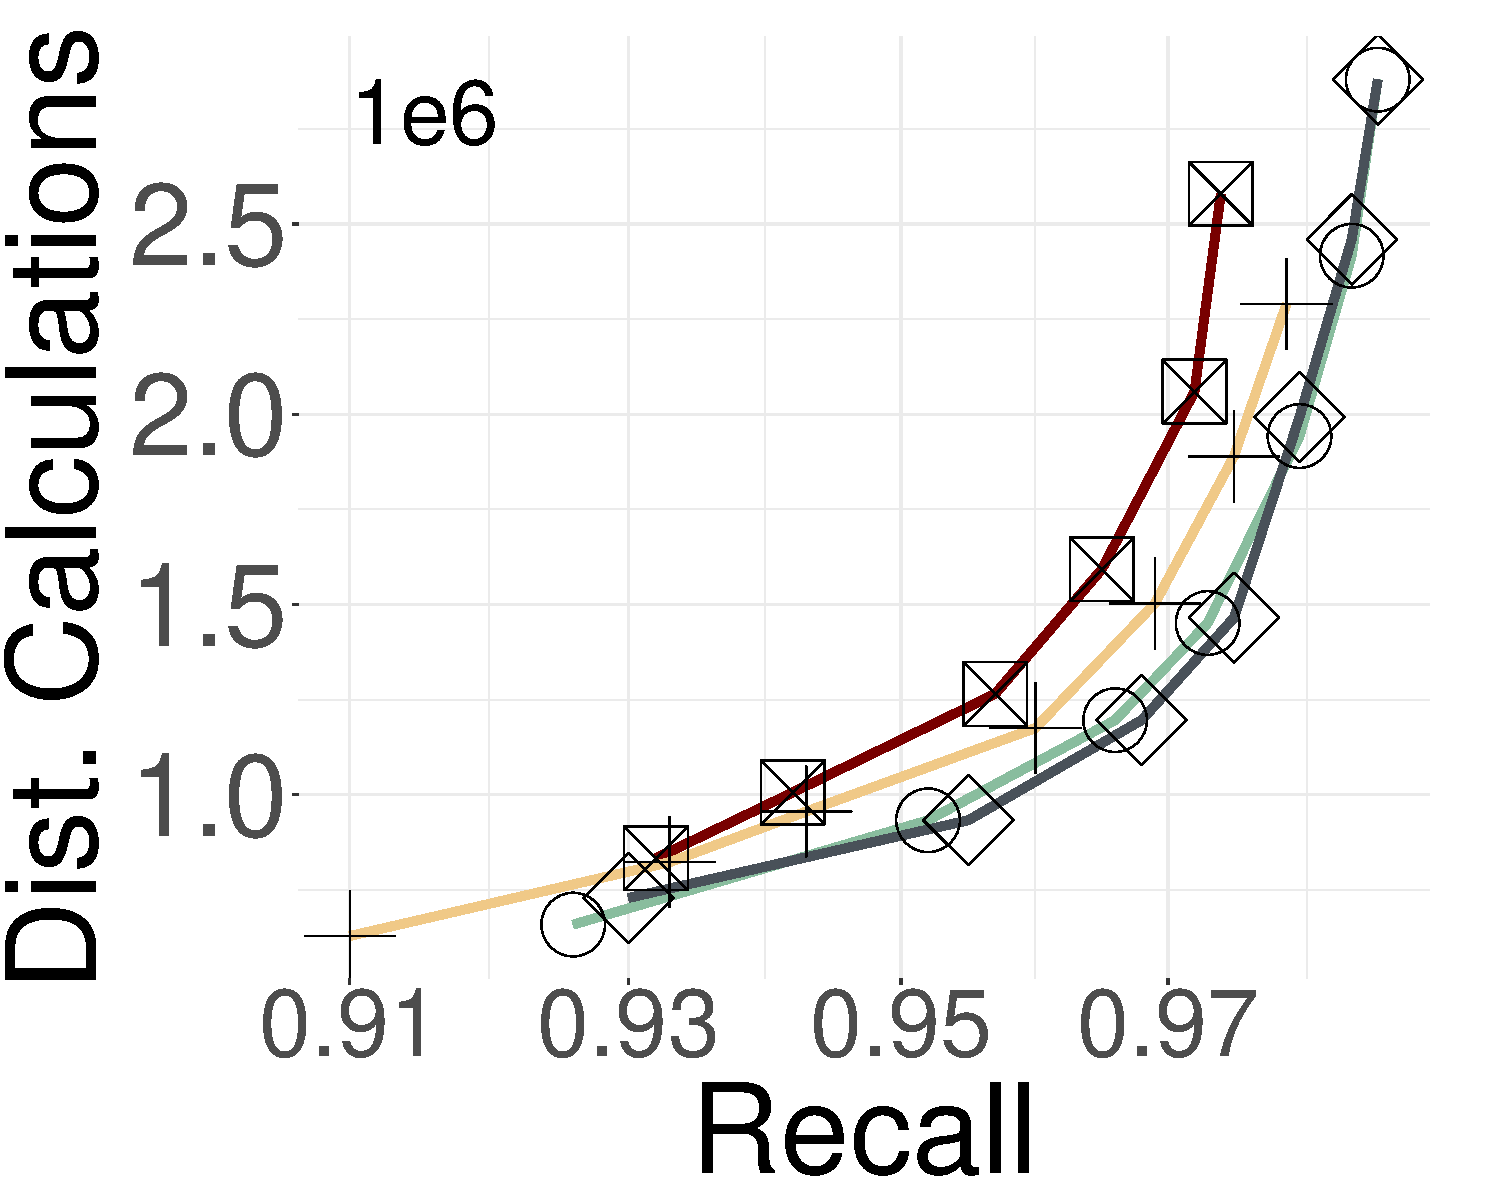
\includegraphics[width=\textwidth]{../img/Experiments/RNG/DC_SIFT1B.pdf}
   \caption{{SIFT1B}}
		\label{fig:ND:sift1b}
		\end{subfigure}	
		\caption{{ND methods performance on real-world datasets}}
		\label{fig:ND:search:real}
 \end{figure}

We compare different ND approaches with II based graph across random dataset with different skewness, Pow1, Pow5 and Pow50 25GB datasets. 

  \noindent{\textbf{Comparison of Query performance on Random Dataset}} Figure~\ref{fig:RNG:search:pow} shows that the three ND strategies have comparable performance when the data distribution is uniform (Pow1), but when the distribution is skewed, MOND takes the lead and RRND becomes competitive with RND. We believe that MOND exhibits a superior performance because on the highly-skewed datasets, the distribution is concentrated within a specific region, thus the orientation pruning of MOND becomes more effective.


\begin{figure}[h!]
	\captionsetup{justification=centering}
	\centering	
		\begin{subfigure}{\columnwidth}
			\centering
			\captionsetup{justification=centering}	
			
\includegraphics[width=0.4\columnwidth]{../img/Experiments/RNG/legend.png}
			\label{fig:RNG:legend}
		\end{subfigure}\\
		\begin{subfigure}{0.28\columnwidth}
			\centering
			\captionsetup{justification=centering}	
			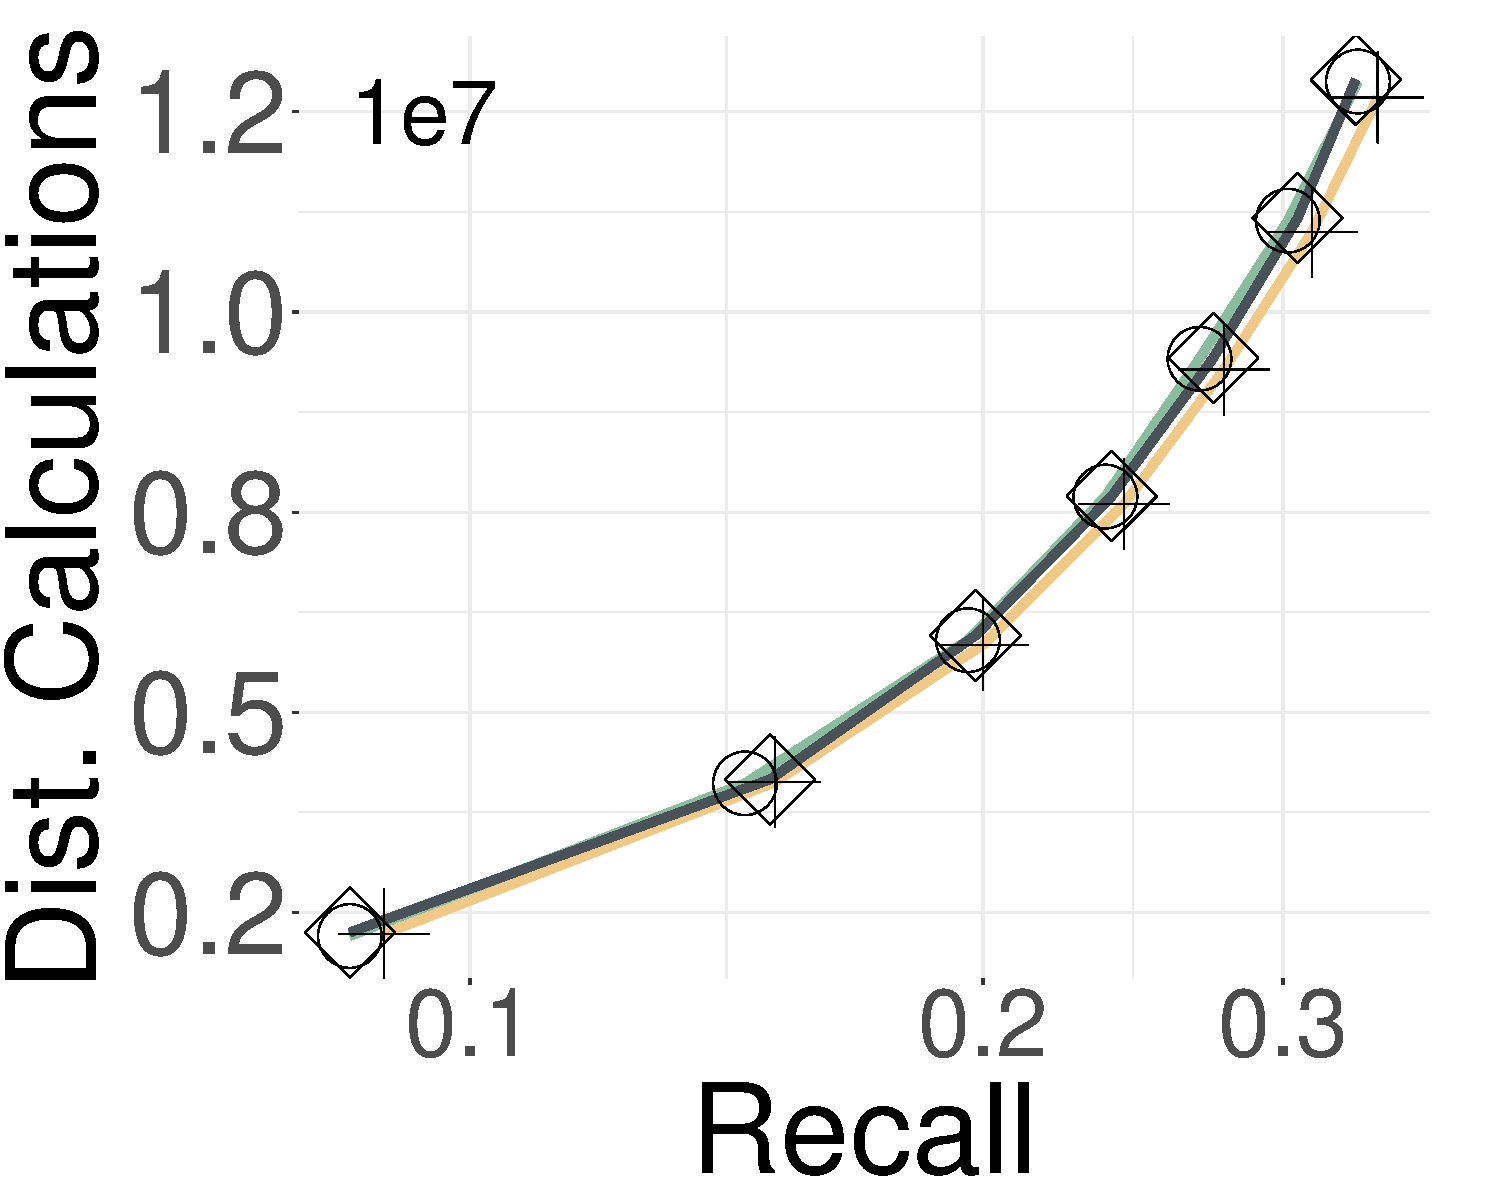
\includegraphics[width=\textwidth]{../img/Experiments/RNG/DC_POW1.pdf}
		\caption{{Pow1}}
		\label{fig:RNG:pow1}
		\end{subfigure}	
  \hspace{0.5cm}
    		\begin{subfigure}{0.28\columnwidth}
			\centering
			\captionsetup{justification=centering}	
				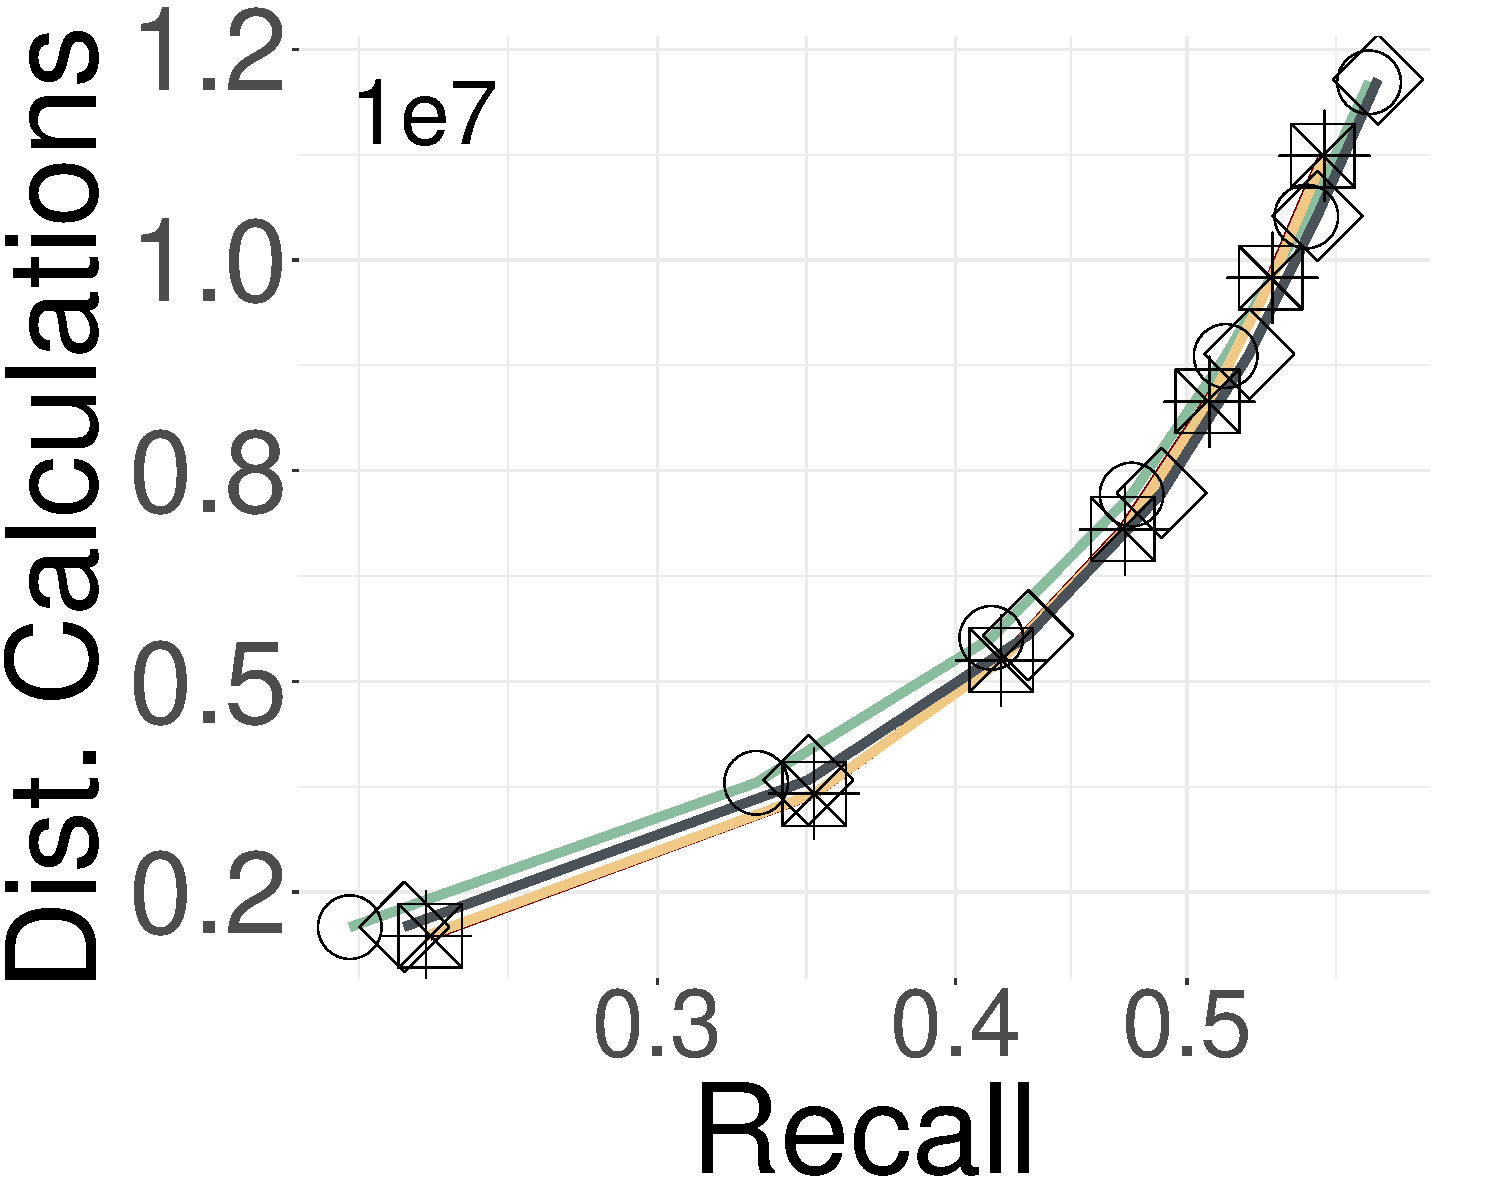
\includegraphics[width=\textwidth]{../img/Experiments/RNG/DC_POW5n.pdf}
		\caption{{Pow5}}
		\label{fig:RNG:deep100GB}
		\end{subfigure}	
  \hspace{0.5cm}
		\begin{subfigure}{0.28\columnwidth}
			\centering
			\captionsetup{justification=centering}	
				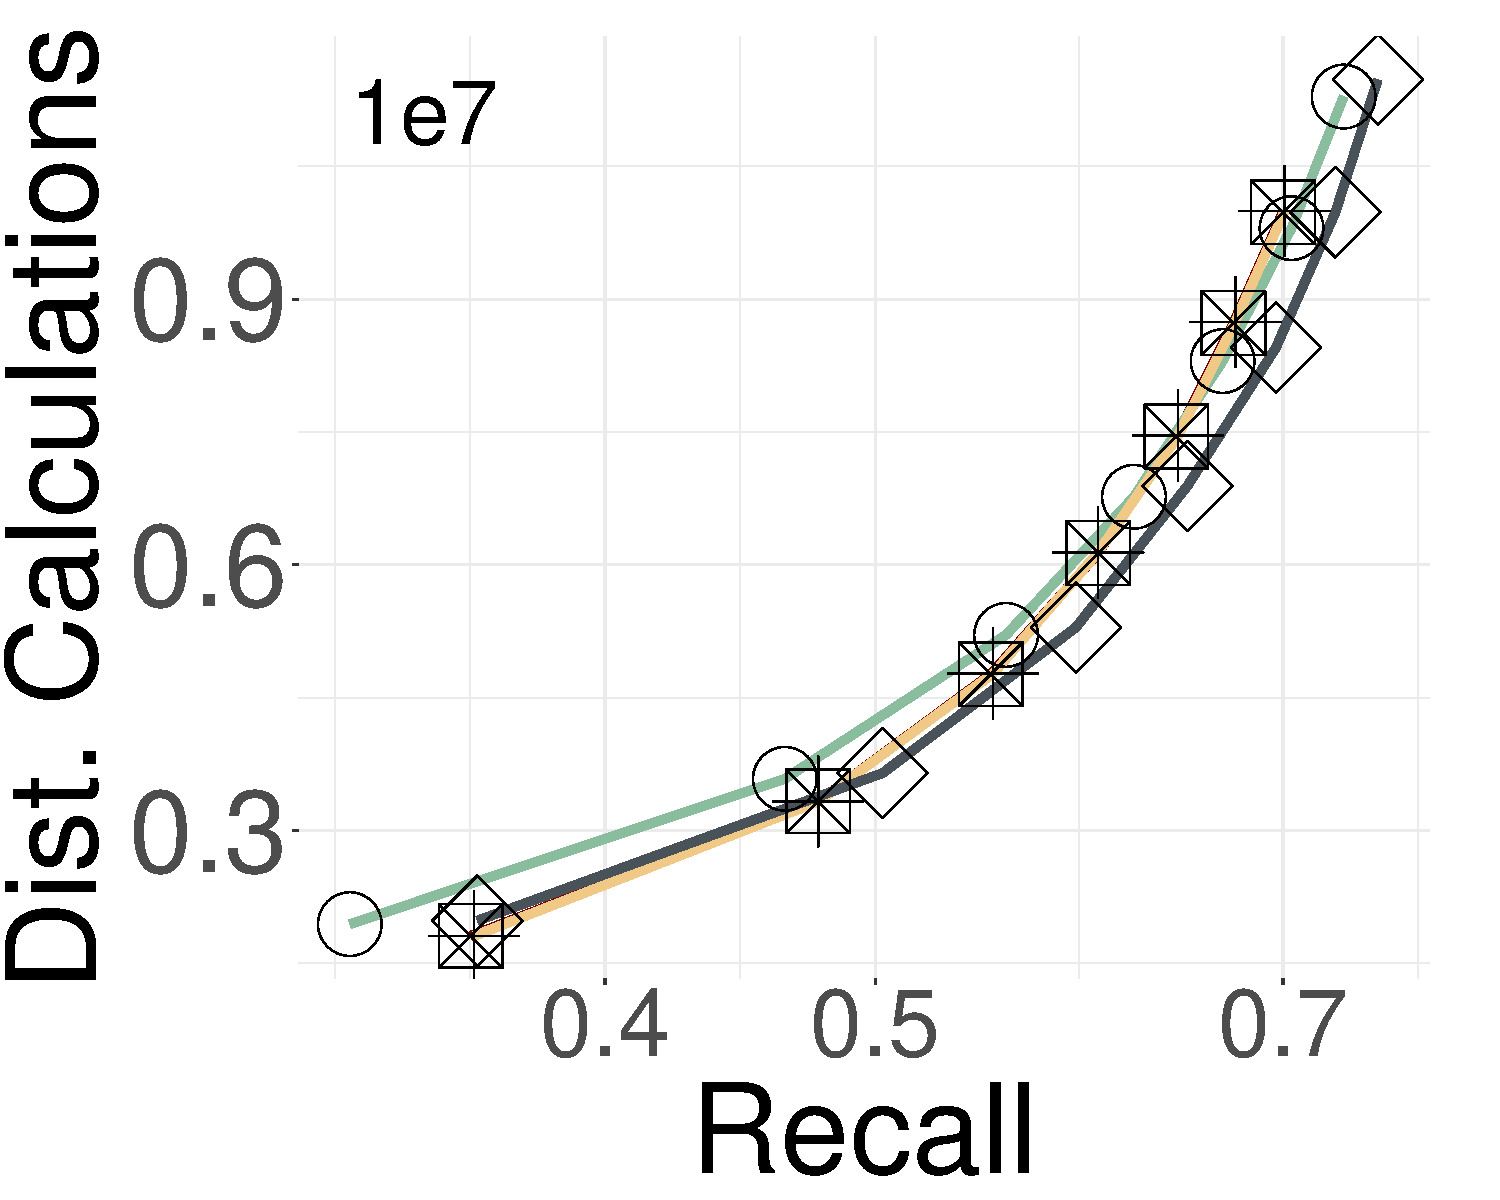
\includegraphics[width=\textwidth]{../img/Experiments/RNG/DC_POW50n.pdf}
		\caption{{Pow50}}
		\label{fig:RNG:pow50}	
  \end{subfigure}	
		\caption{{ND methods performance on random datasets}}
		\label{fig:RNG:search:pow}

 \end{figure}

\subsection{Seed Selection}
In this set of experiments, we evaluate four of the most frequently used Seed Selection (SS) strategies for the beam search algorithm: SN~\cite{hnsw,elpis}, MD~\cite{nsg,vamana}, KS~\cite{kgraph,nsw11,dpg,vamana,nssg}, and KD~\cite{efanna,SPTAG1,hcnng} (note that KM and LSH are excluded as they are not commonly used in graph-based methods). We also include the baseline method SF, which, while not previously applied in the literature, serves as a reference. Each SS strategy is tested using the same graph structure based on Incremental Insertion (II) and RND pruning, which we have identified as the most effective configuration in Section~\ref{subsec:experiments-ND}.

We conduct 100 query experiments for each strategy across the Deep and Sift datasets at sizes of 25GB, 100GB, and 1B. Extrapolating the results to 1M queries, we report the number of distance calculations required to achieve 0.99 recall in Figure~\ref{fig:ss:search}. SN and KS are shown to be the most efficient strategies overall, while SF and MD are the least efficient. The KD strategy demonstrates competitive performance on the 25GB and 100GB datasets, but its performance declines on larger billion-scale datasets. 

KS outperforms SN on smaller datasets (25GB and 100GB); however, this trend reverses on the 1B dataset, where SN becomes more efficient. The difference in distance calculations between SN and KS is approximately 1M on the 25GB dataset and around 10M on the 1B dataset. As the dataset size grows, it becomes necessary to sample more nodes (beyond the beam width used during KS searches) to better represent the dataset and improve the chances of starting the search in a region closer to the query (SN adjusts its sample size logarithmically with dataset size, improving its performance). Figure~\ref{fig:ss:search} also indicates that MD and SF consistently rank among the least efficient strategies, with MD outperforming SF on Deep, but SF surpassing MD on Sift. This suggests that neither MD nor SF is particularly effective or reliable for seed selection.

Next, we analyze how SS strategies affect index construction. We focus on the two best-performing strategies, KS and SN, and study their impact on the same II and RND baseline~\cite{nsw11,dpg,hnsw,nsg,nssg,vamana,elpis,SPTAG1}. These methods are most influenced by the SS strategy, as they use a beam search, which includes seed selection during node insertion.

We build indices using each strategy on the Deep1M and Deep25GB datasets and measure the associated distance calculations. Additionally, we calculate the distance overhead of SN compared to KS, estimating the number of additional 100-NN queries the KS-based graph can answer (with 0.99 recall) before the SN-based graph completes construction.

The results are presented in Table~\ref{tab:ss:idx}. We observe that building the SN-based graph incurs 182 million and 22.3 billion more distance calculations than the KS-based graph on Deep1M and Deep25GB, respectively. Furthermore, the KS-based graph can answer approximately 45K and 1.17 million queries on Deep1M and Deep25GB, respectively, before the SN-based graph finishes its construction.


\newcommand{\sfig}{0.28}
\newcommand{\spbfig}{0.3}

\begin{figure}[htp]
	\captionsetup{justification=centering}
	\centering	
 		\begin{subfigure}{0.018\columnwidth}
			\centering
			\captionsetup{justification=centering}	
			
\includegraphics[width=\textwidth]{img/Experiments/EP/dc.png}
   \vspace{0.18in}
		\end{subfigure}	
		\begin{subfigure}{\sfig\columnwidth}
			\centering
			\captionsetup{justification=centering}	
			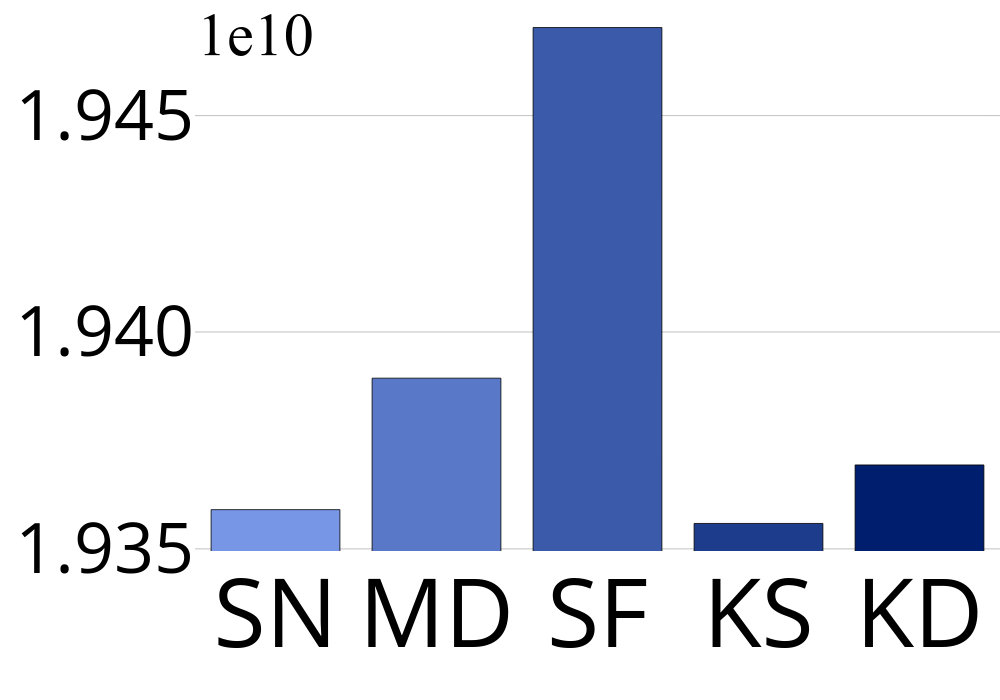
\includegraphics[width=\textwidth]{../img/Experiments/EP/DEEP_25GB_100.png}
		\caption{{Deep25GB}}
		\label{fig:ss:deep1b}
		\end{subfigure}	
	%	\captionsetup{justification=centering}
		\begin{subfigure}{\sfig\columnwidth}
			\centering
			\captionsetup{justification=centering}	
			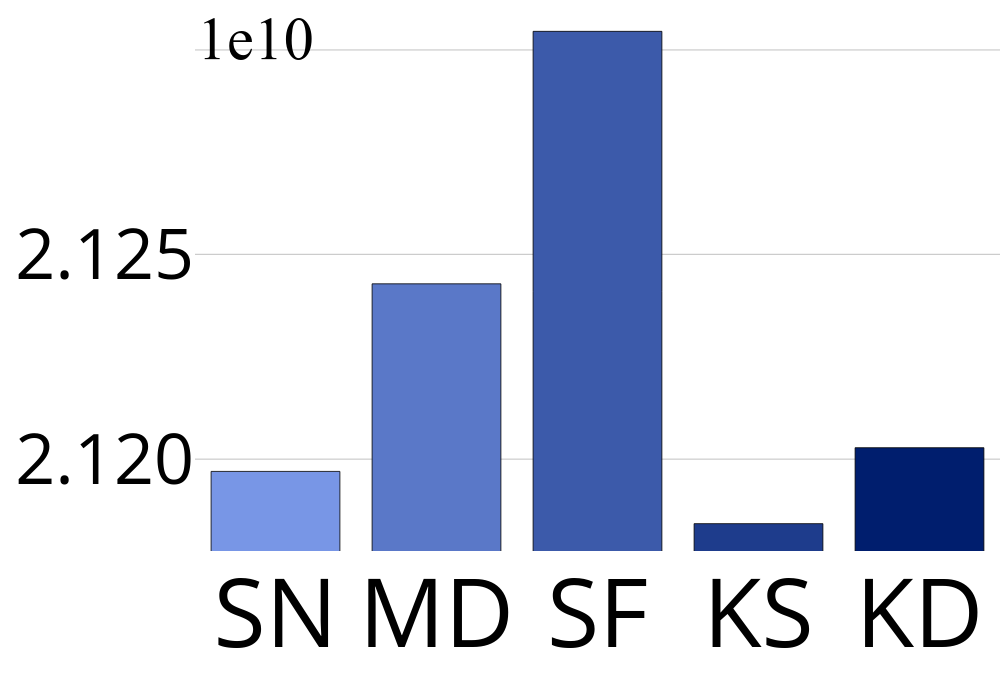
\includegraphics[width=\textwidth]{../img/Experiments/EP/DEEP_100GB_100.png}
		\caption{{Deep100GB}}
		\label{fig:ss:deep1b}
		\end{subfigure}		
		\begin{subfigure}{\sfig\columnwidth}
			\centering
			\captionsetup{justification=centering}	
			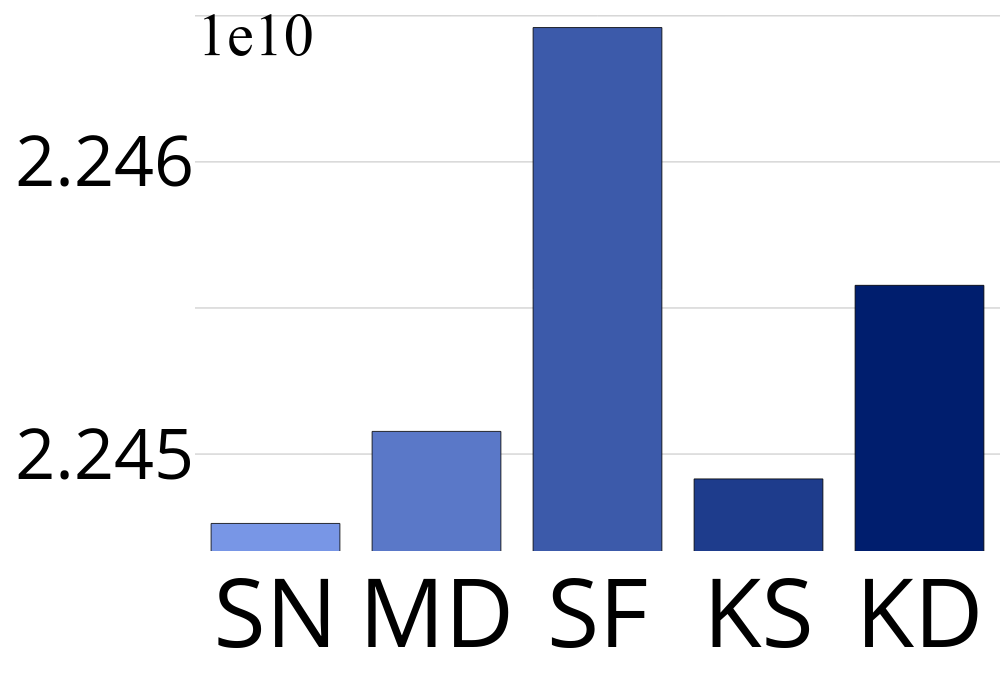
\includegraphics[width=\textwidth]{../img/Experiments/EP/DEEP_1B_100.png}
		\caption{{Deep1B}}
		\label{fig:ss:deep1b}
		\end{subfigure}	

	\begin{subfigure}{0.018\columnwidth}
			\centering
			\captionsetup{justification=centering}	
			
\includegraphics[width=\textwidth]{img/Experiments/EP/dc.png}
   \vspace{0.2in}
		\end{subfigure}	
		\begin{subfigure}{\sfig\columnwidth}
			\centering
			\captionsetup{justification=centering}	
			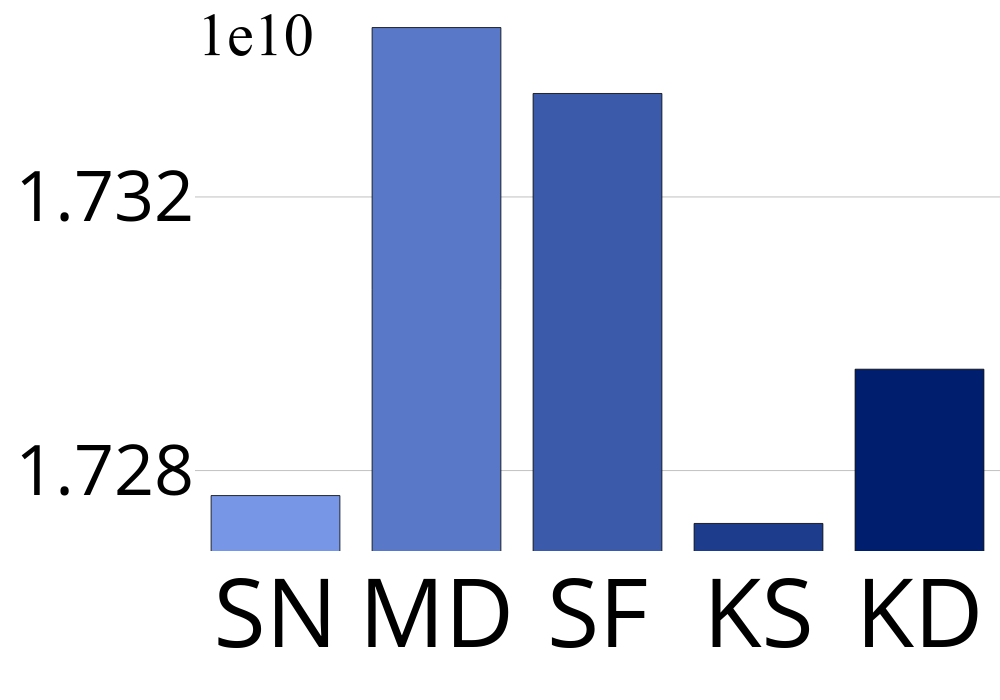
\includegraphics[width=\textwidth]{../img/Experiments/EP/SIFT_25GB_100.png}
		\caption{{Sift25GB}}
		\label{fig:ss:sift1b}
		\end{subfigure}	
	%	\captionsetup{justification=centering}
		\begin{subfigure}{\sfig\columnwidth}
			\centering
			\captionsetup{justification=centering}	
			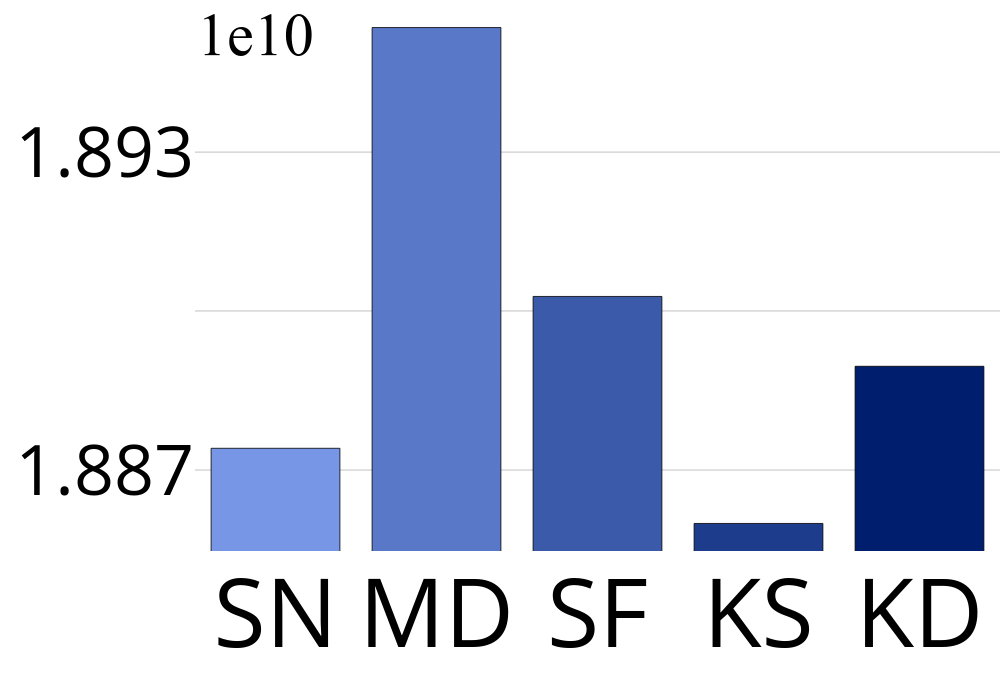
\includegraphics[width=\textwidth]{../img/Experiments/EP/SIFT_100GB_100.png}
		\caption{{Sift100GB}}
		\label{fig:ss:sift1b}
		\end{subfigure}		
		\begin{subfigure}{\sfig\columnwidth}
			\centering
			\captionsetup{justification=centering}	
			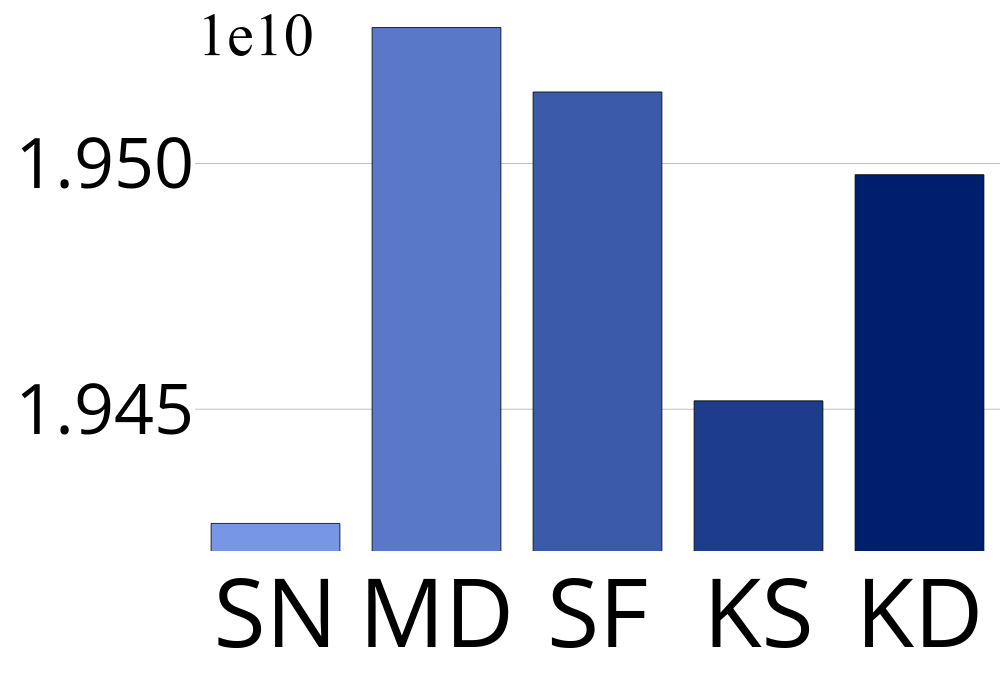
\includegraphics[width=\textwidth]{../img/Experiments/EP/SIFT_1B_100.png}
		\caption{{Sift1B}}
		\label{fig:ss:sift1b}
		\end{subfigure}	
\caption{The impact of SS Methods on Query Answering}
\label{fig:ss:search}
 \end{figure}
 


\begin{table}[h!]
\centering
\begin{tabular}{@{}lcc@{}}
\toprule
%\textbf{Metric} 
& \textbf{Deep1M} & \textbf{Deep25GB} \\ 
\midrule
\textbf{Dist. Calculations (SN)} & 4.3 billion & 1.49 trillion \\
\textbf{Dist. Calculations (KS)} & 4.1 billion & 1.46 trillion \\
\midrule
\textbf{Overhead (SN vs. KS)} & 182 million & 22.3 billion \\
\textbf{Additional Queries} & 44,959 & 1,165,870 \\
\bottomrule
\end{tabular}
\caption{The impact of SS methods on Indexing Performance}
\label{tab:ss:idx}
\end{table}

\begin{comment}
    \subsection{Empirical Analysis of the theoretical complexity of Beam search}
\ilias{I have added this subsection to appendix, i think it's better to have it there with also proof of approximations between the NDs approaches}
Beam search, introduced by Raj Reddy in 1977, is a core algorithm widely used across various fields, including speech recognition, machine translation, and natural language processing. It operates by exploring a restricted number of hypotheses, referred to as the "beam," improving efficiency compared to exhaustive search approaches. However, beam search trades off completeness and optimality for speed, as it may prune potential goal states, and thus does not always guarantee finding the best solution. The time complexity of beam search is determined by factors such as the beam width and the maximum allowable path length in the graph. When applied to proximity graphs, as used in spatial data analysis, beam search efficiently explores nearby nodes or edges, making it highly versatile across different domains.

The time complexity of beam search is described by the following formula:

\[
\text{Time Complexity} = O(B \times m \times T) \quad (\text{Eq. 4})
\]

Where \( B \) denotes the beam width, \( m \) represents the average branching factor (or average outdegree in graph search), and \( T \) indicates the maximum path length allowed within the graph. In the worst case, \( T \) is equivalent to the graph's diameter, representing the longest possible path. This formula captures the computational cost of beam search, factoring in the beam width, average outdegree, and graph diameter. However, because the search accuracy for a given beam width is not guaranteed, the exact time complexity can only be approximated by running a search on a query set to determine the necessary beam width for a target accuracy. Sometimes, the differences in beam widths between methods may have a greater impact on time complexity than variations in outdegree or diameter. It is also worth noting that different seed selection strategies can affect time complexity, especially when the number of nearest neighbors required is small.

Below, we provide an analysis of the theoretical time complexity and its alignment with the empirical performance of four state-of-the-art graph-based algorithms. For each method, the graph is built with maximum outdegrees of 40, 40, 50, and 60 for the datasets Deep1M, Deep2M, Deep4M, and Deep8M, respectively. The purpose is to examine how the theoretical time complexity corresponds to the empirical performance of the methods, both in terms of time and the number of distance calculations. All measurements are taken for a target accuracy of 0.99.

\begin{figure}
\centering
\begin{subfigure}{0.45\textwidth}
  \centering
  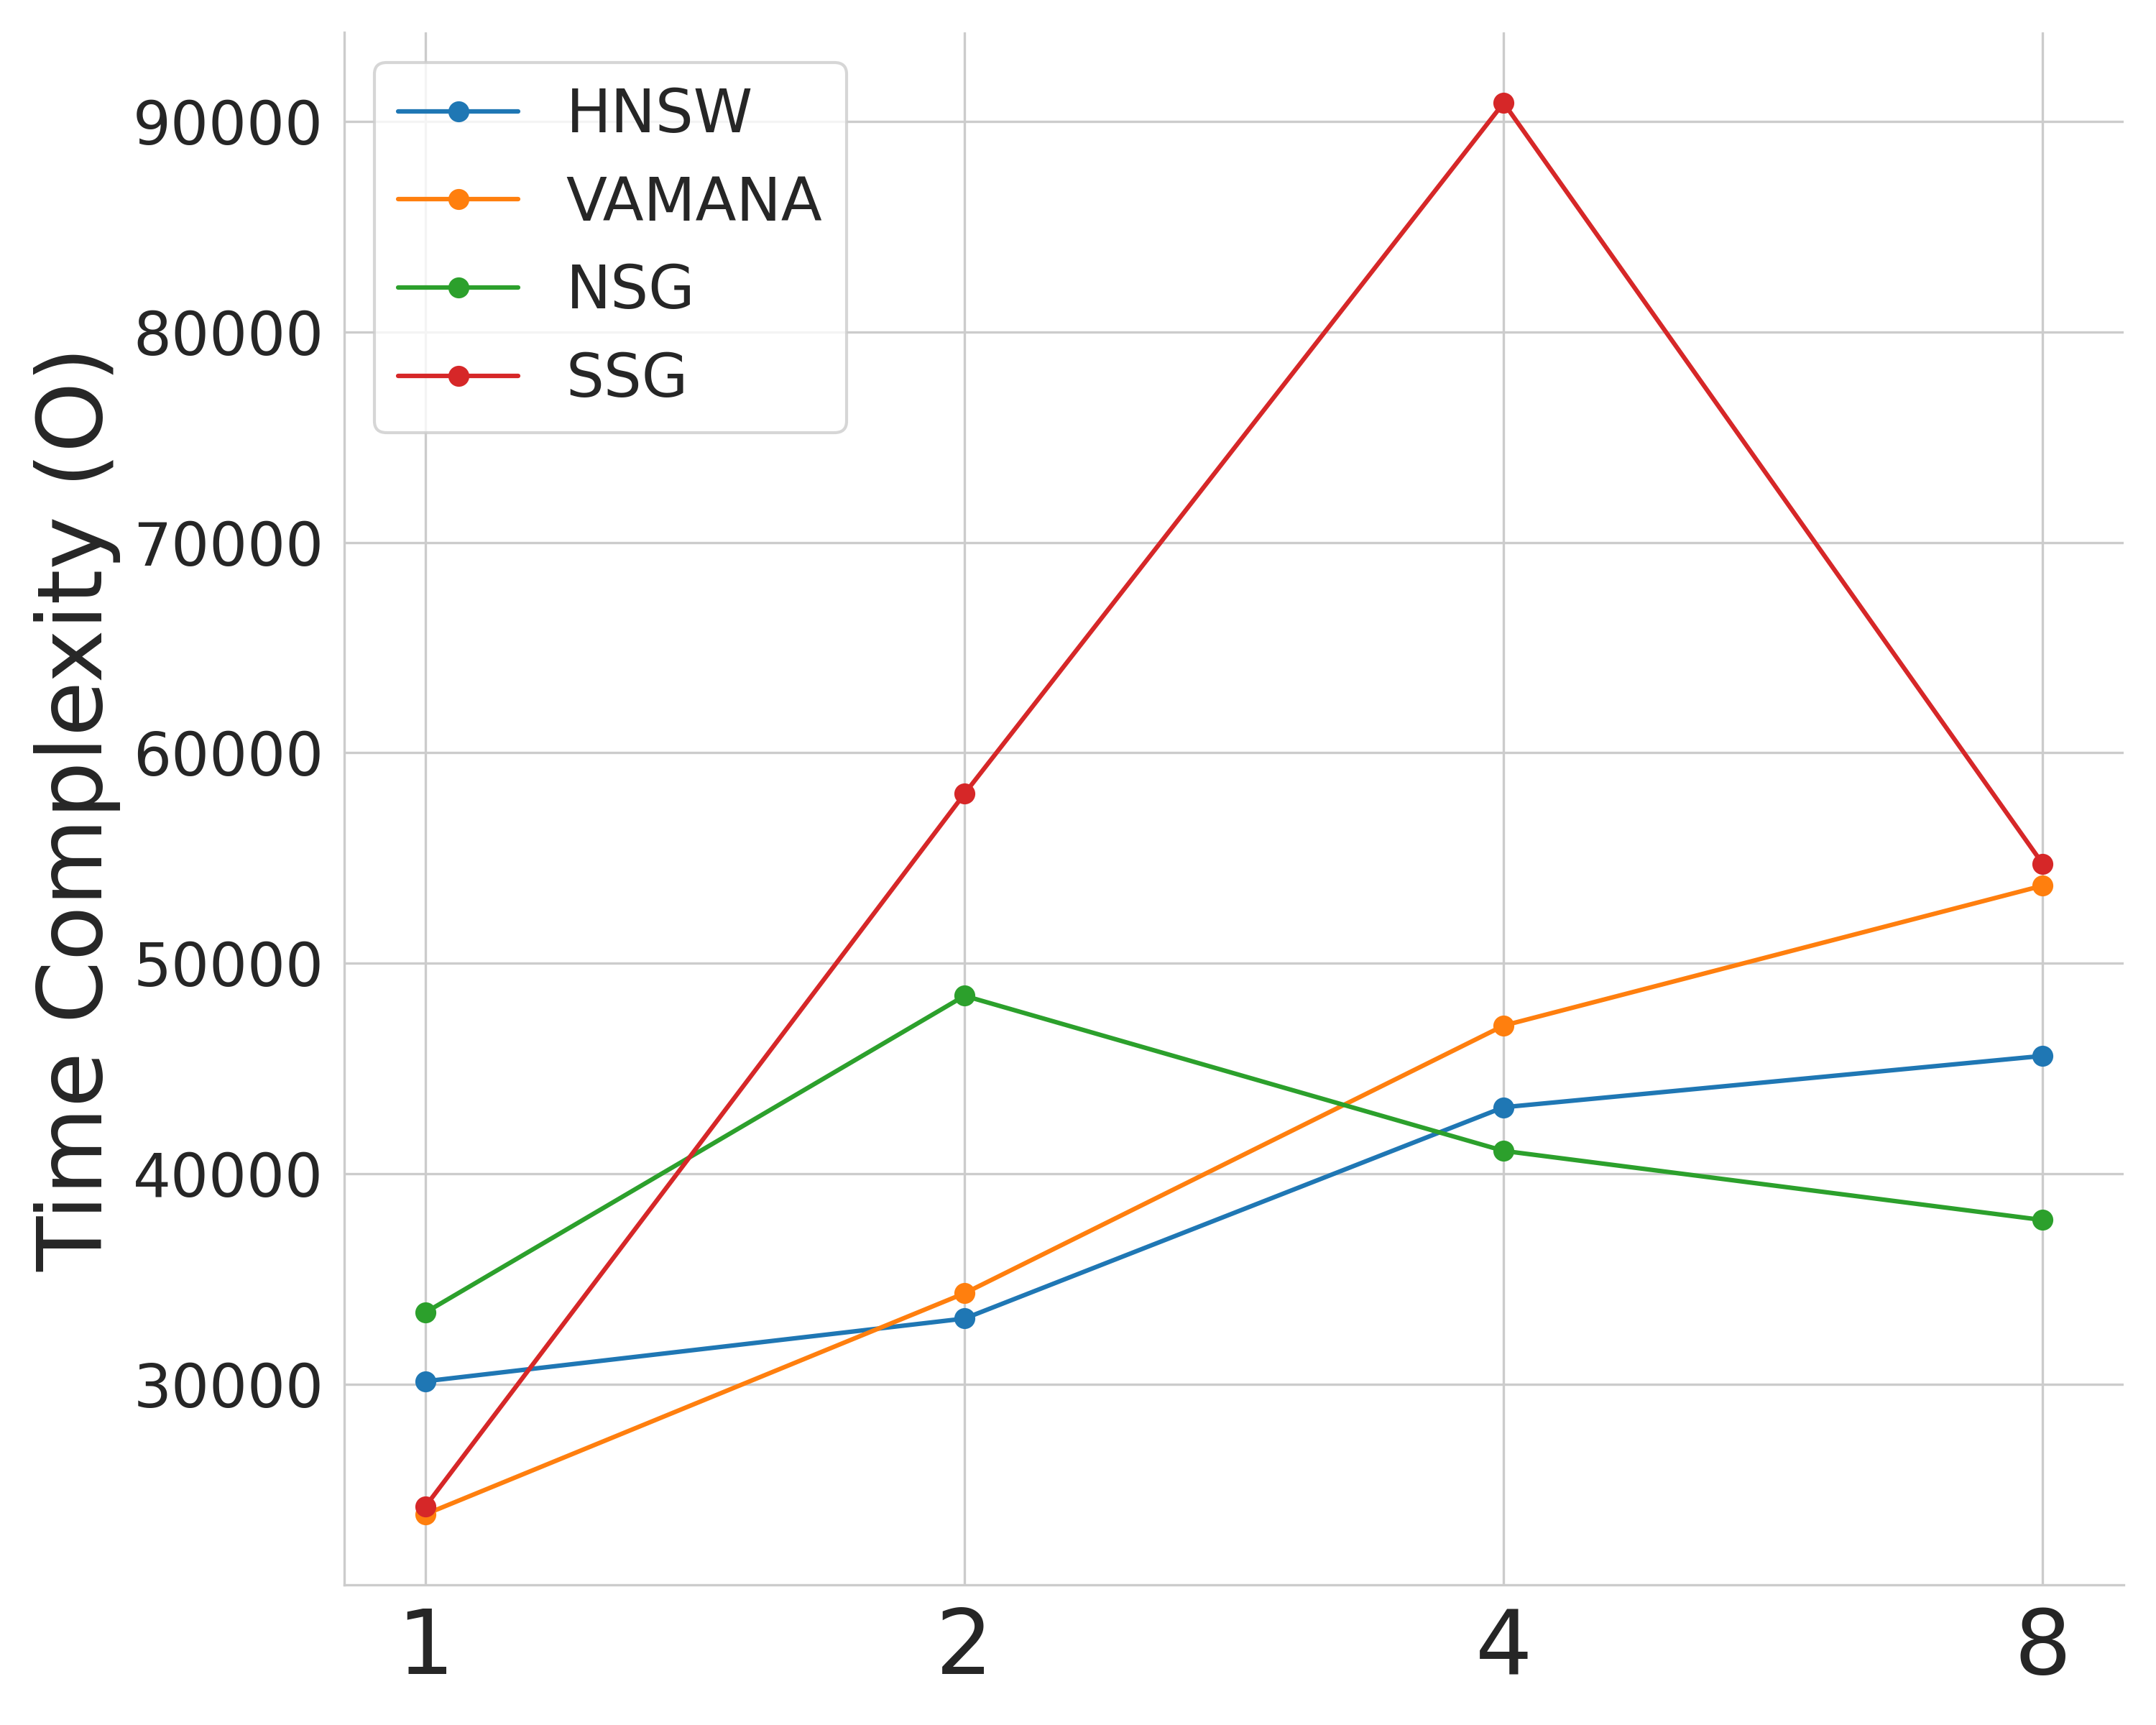
\includegraphics[width=\linewidth]{../img/Experiments/BSC/complexity_size.png}
  \caption{Theoretical Time Complexity}
  \label{fig:cno}
\end{subfigure}
\hfill
\begin{subfigure}{0.45\textwidth}
  \centering
  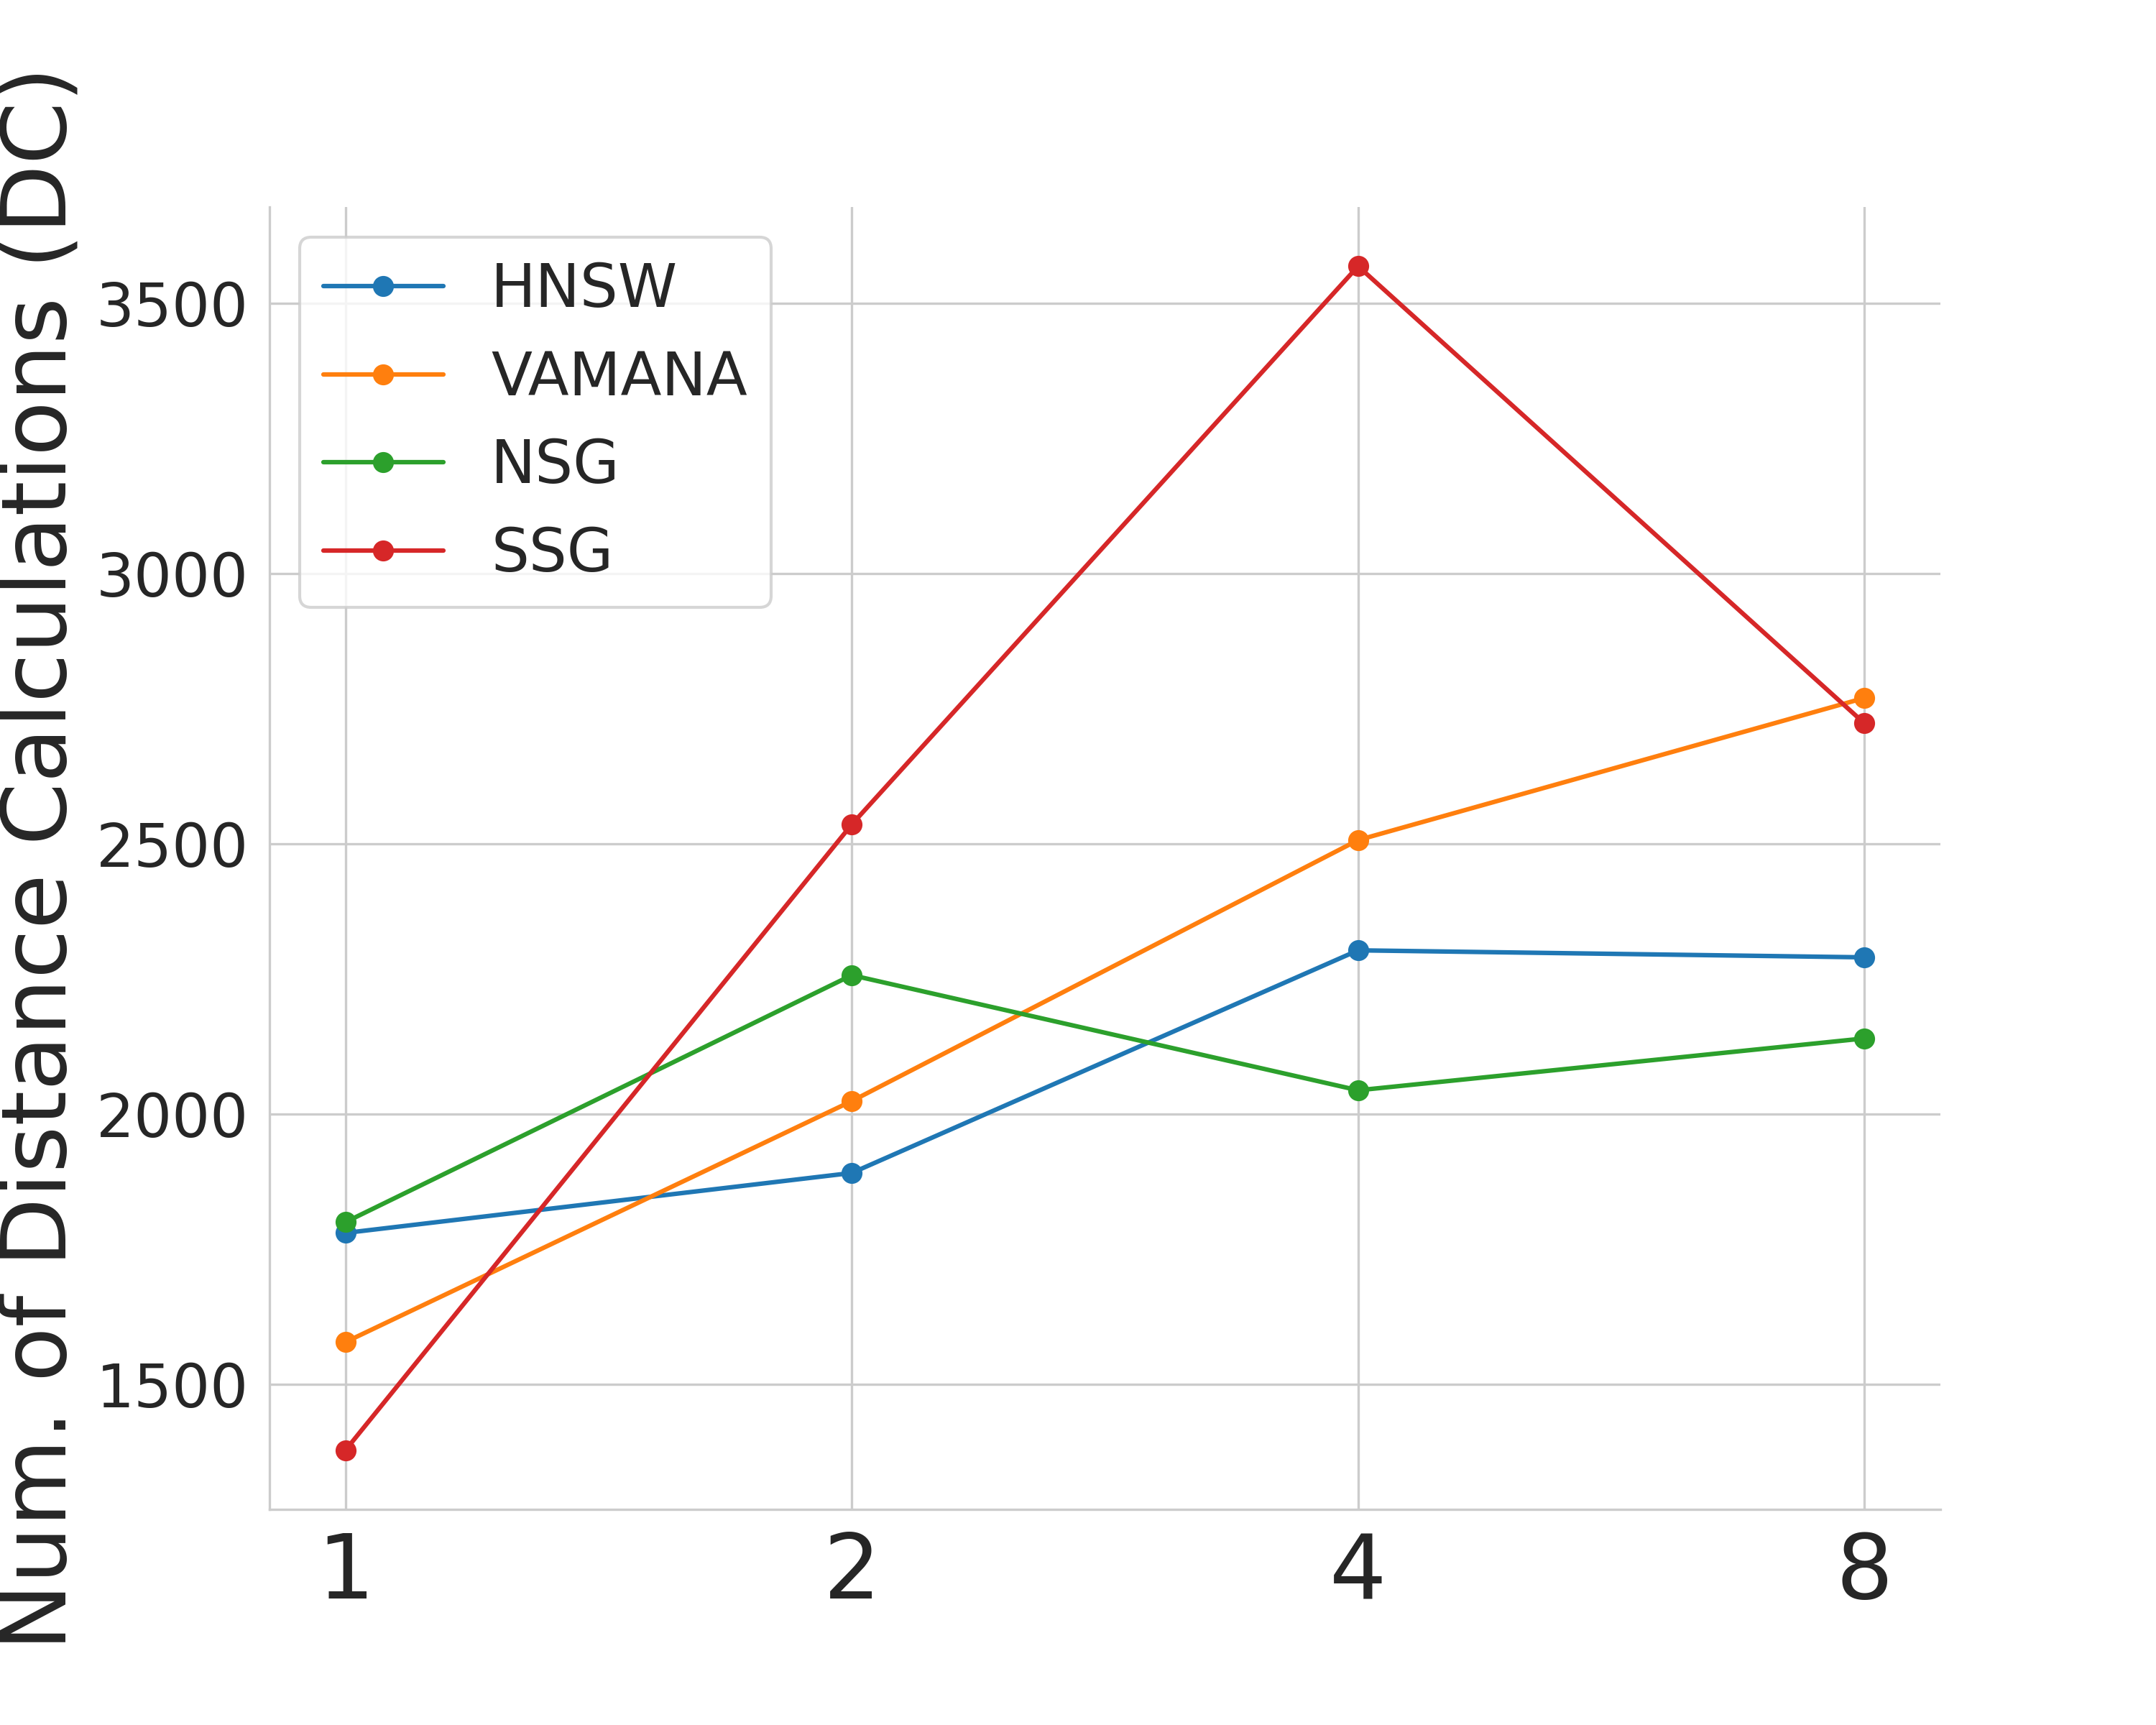
\includegraphics[width=\linewidth]{../img/Experiments/BSC/dc_size.png}
  \caption{Empirical efficiency}
  \label{fig:dc}
\end{subfigure}
\caption{Theoretical and empirical beams search efficiency across different deep1b dataset sizes}
\label{fig:ndc_no_size_plots}
\end{figure}

In Figure ~\ref{fig:ndc_no_size_plots}, we illustrate how the theoretical time complexity of the beam search aligns with the algorithm efficiency, specifically the number of distance calculations across different dataset sizes. As the dataset size increases, we can observe an improvement in the approximation of the empirical complexity (comparing 1M to 2M, 4M, and 8M), as the ranking between methods in terms of beam search efficiency is approximated using the beam search time complexity formula in Eq. 4.
In Figure ~\ref{fig:ndc_no_plots}, we present the comparison between the time complexity and search efficiency of four methods for different deep1b dataset scales.

\begin{figure}[htbp]
\centering
\begin{subfigure}{0.24\textwidth}
  \centering
  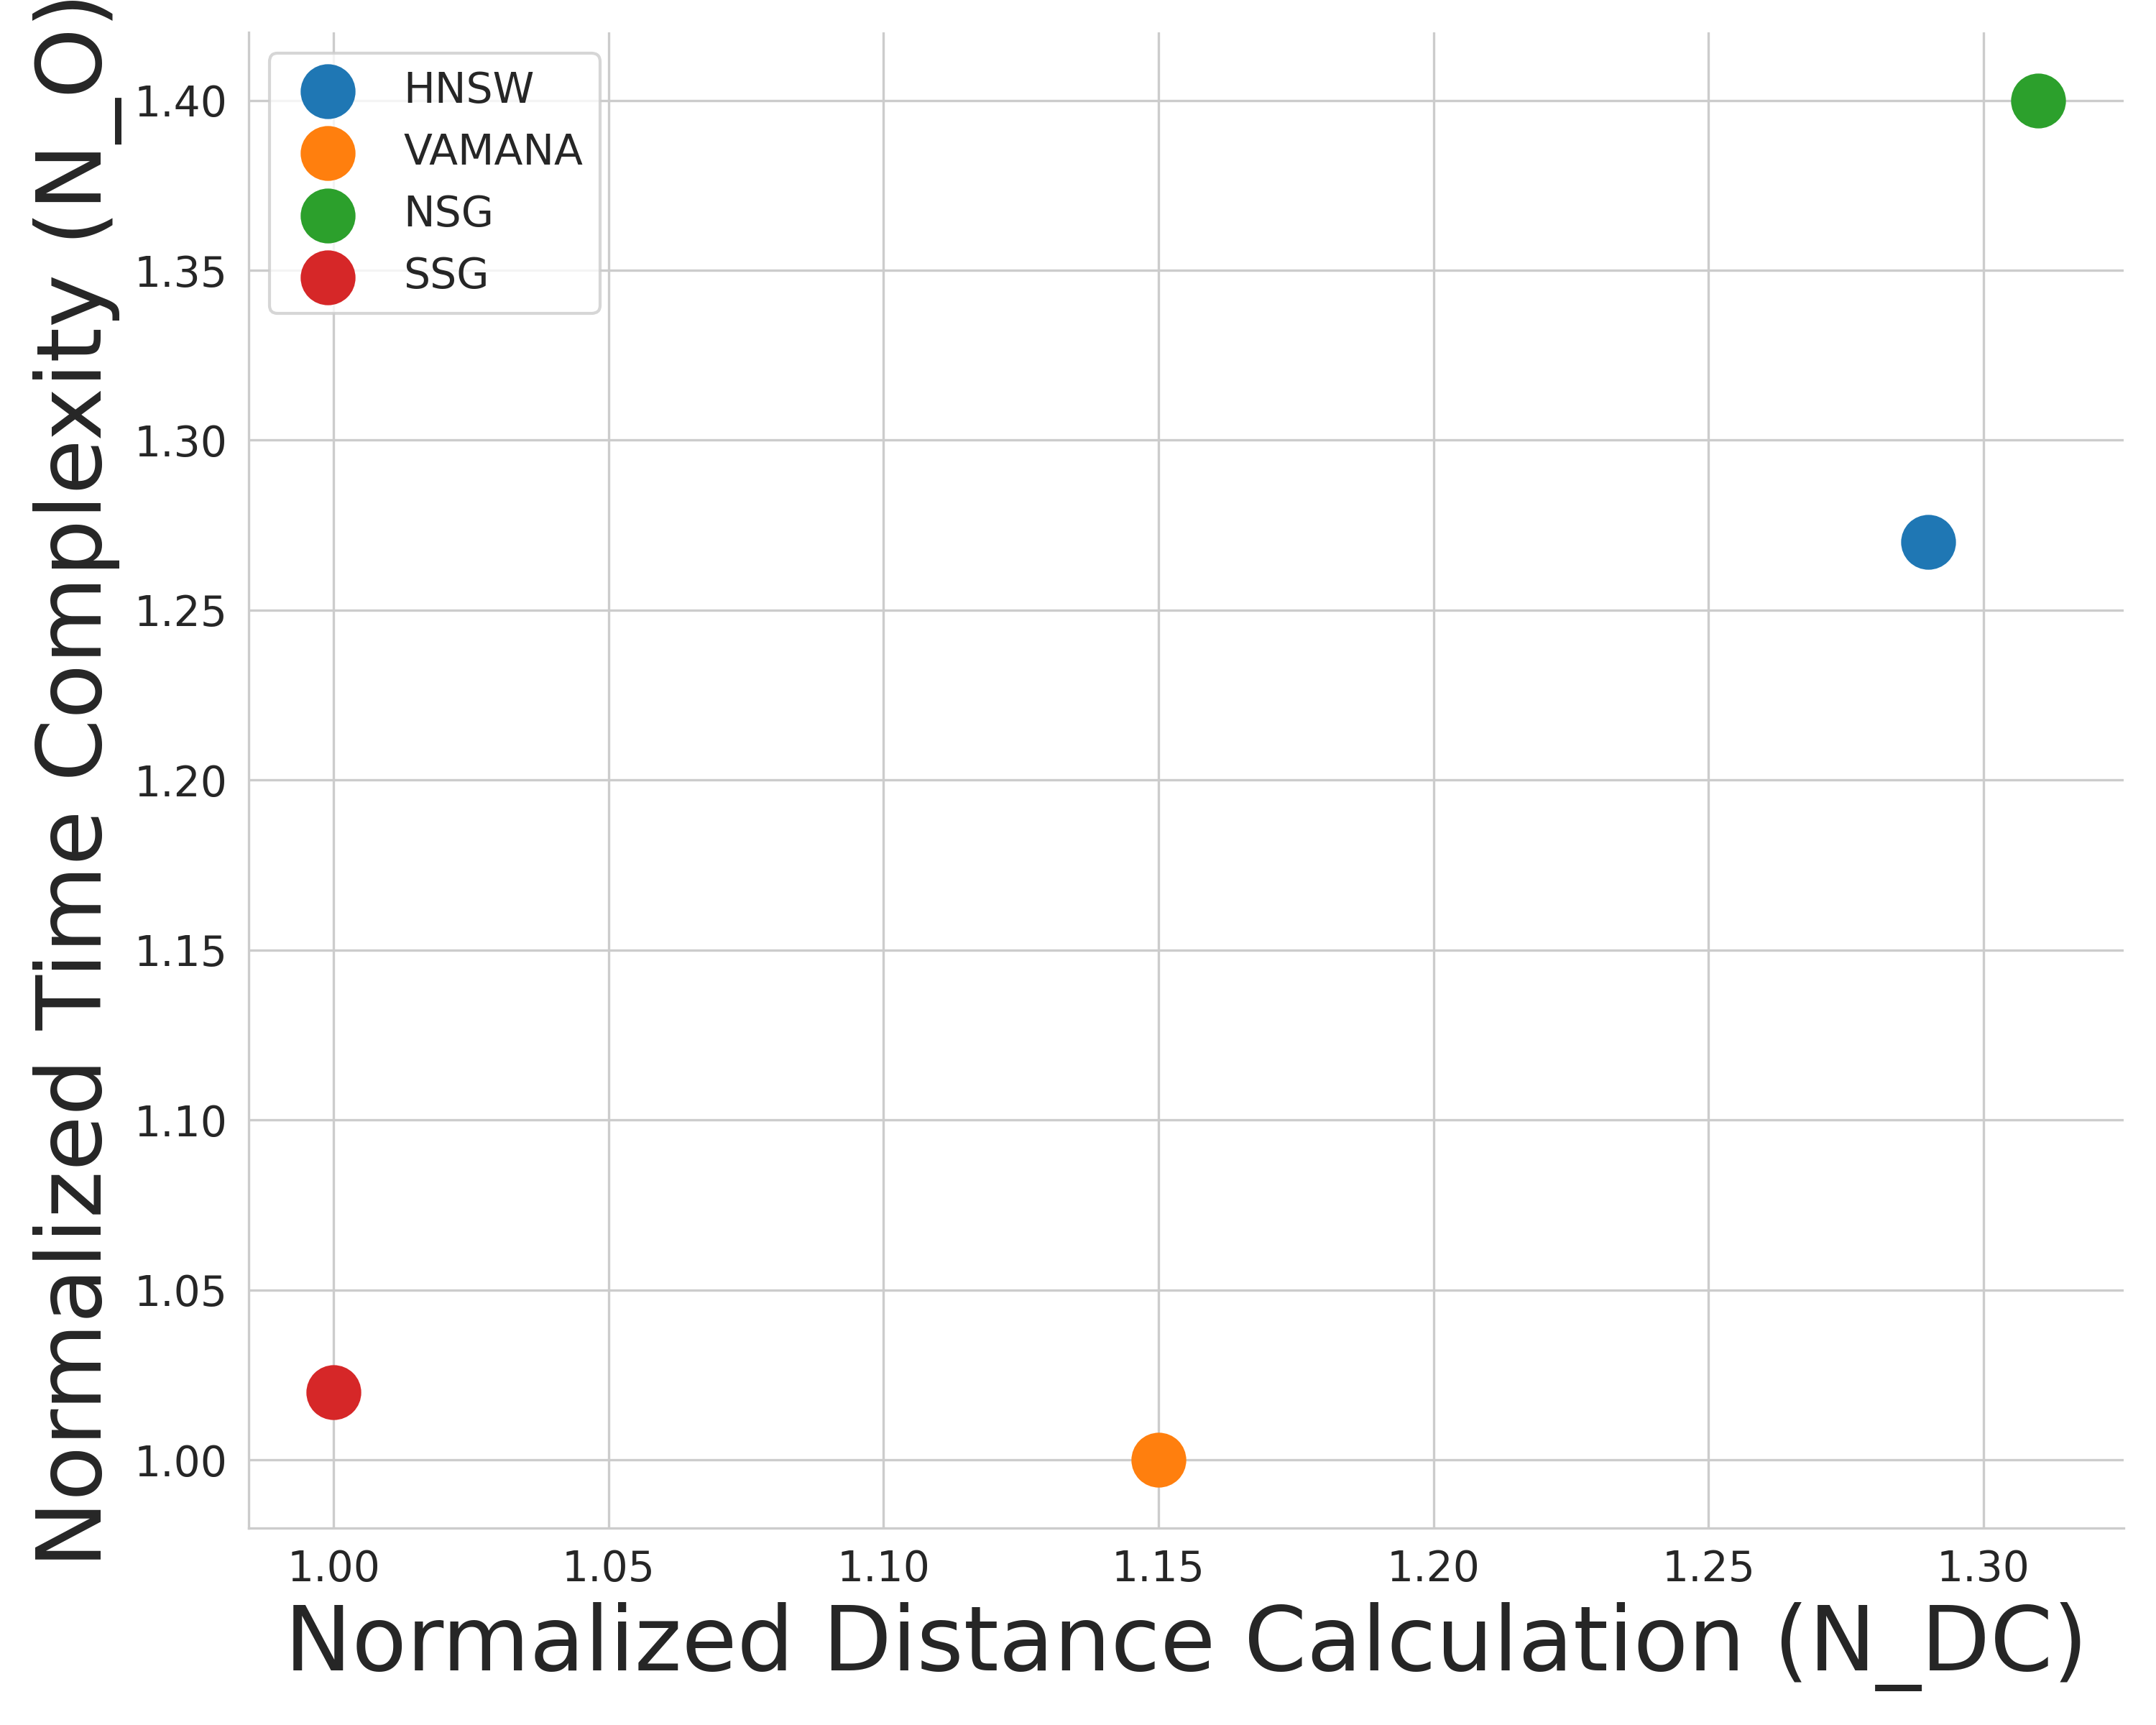
\includegraphics[width=\linewidth]{../img/Experiments/BSC/1_ndc_no.png}
  \caption{Deep1M}
  \label{fig:1_ndc_no}
\end{subfigure}
\hfill
\begin{subfigure}{0.24\textwidth}
  \centering
  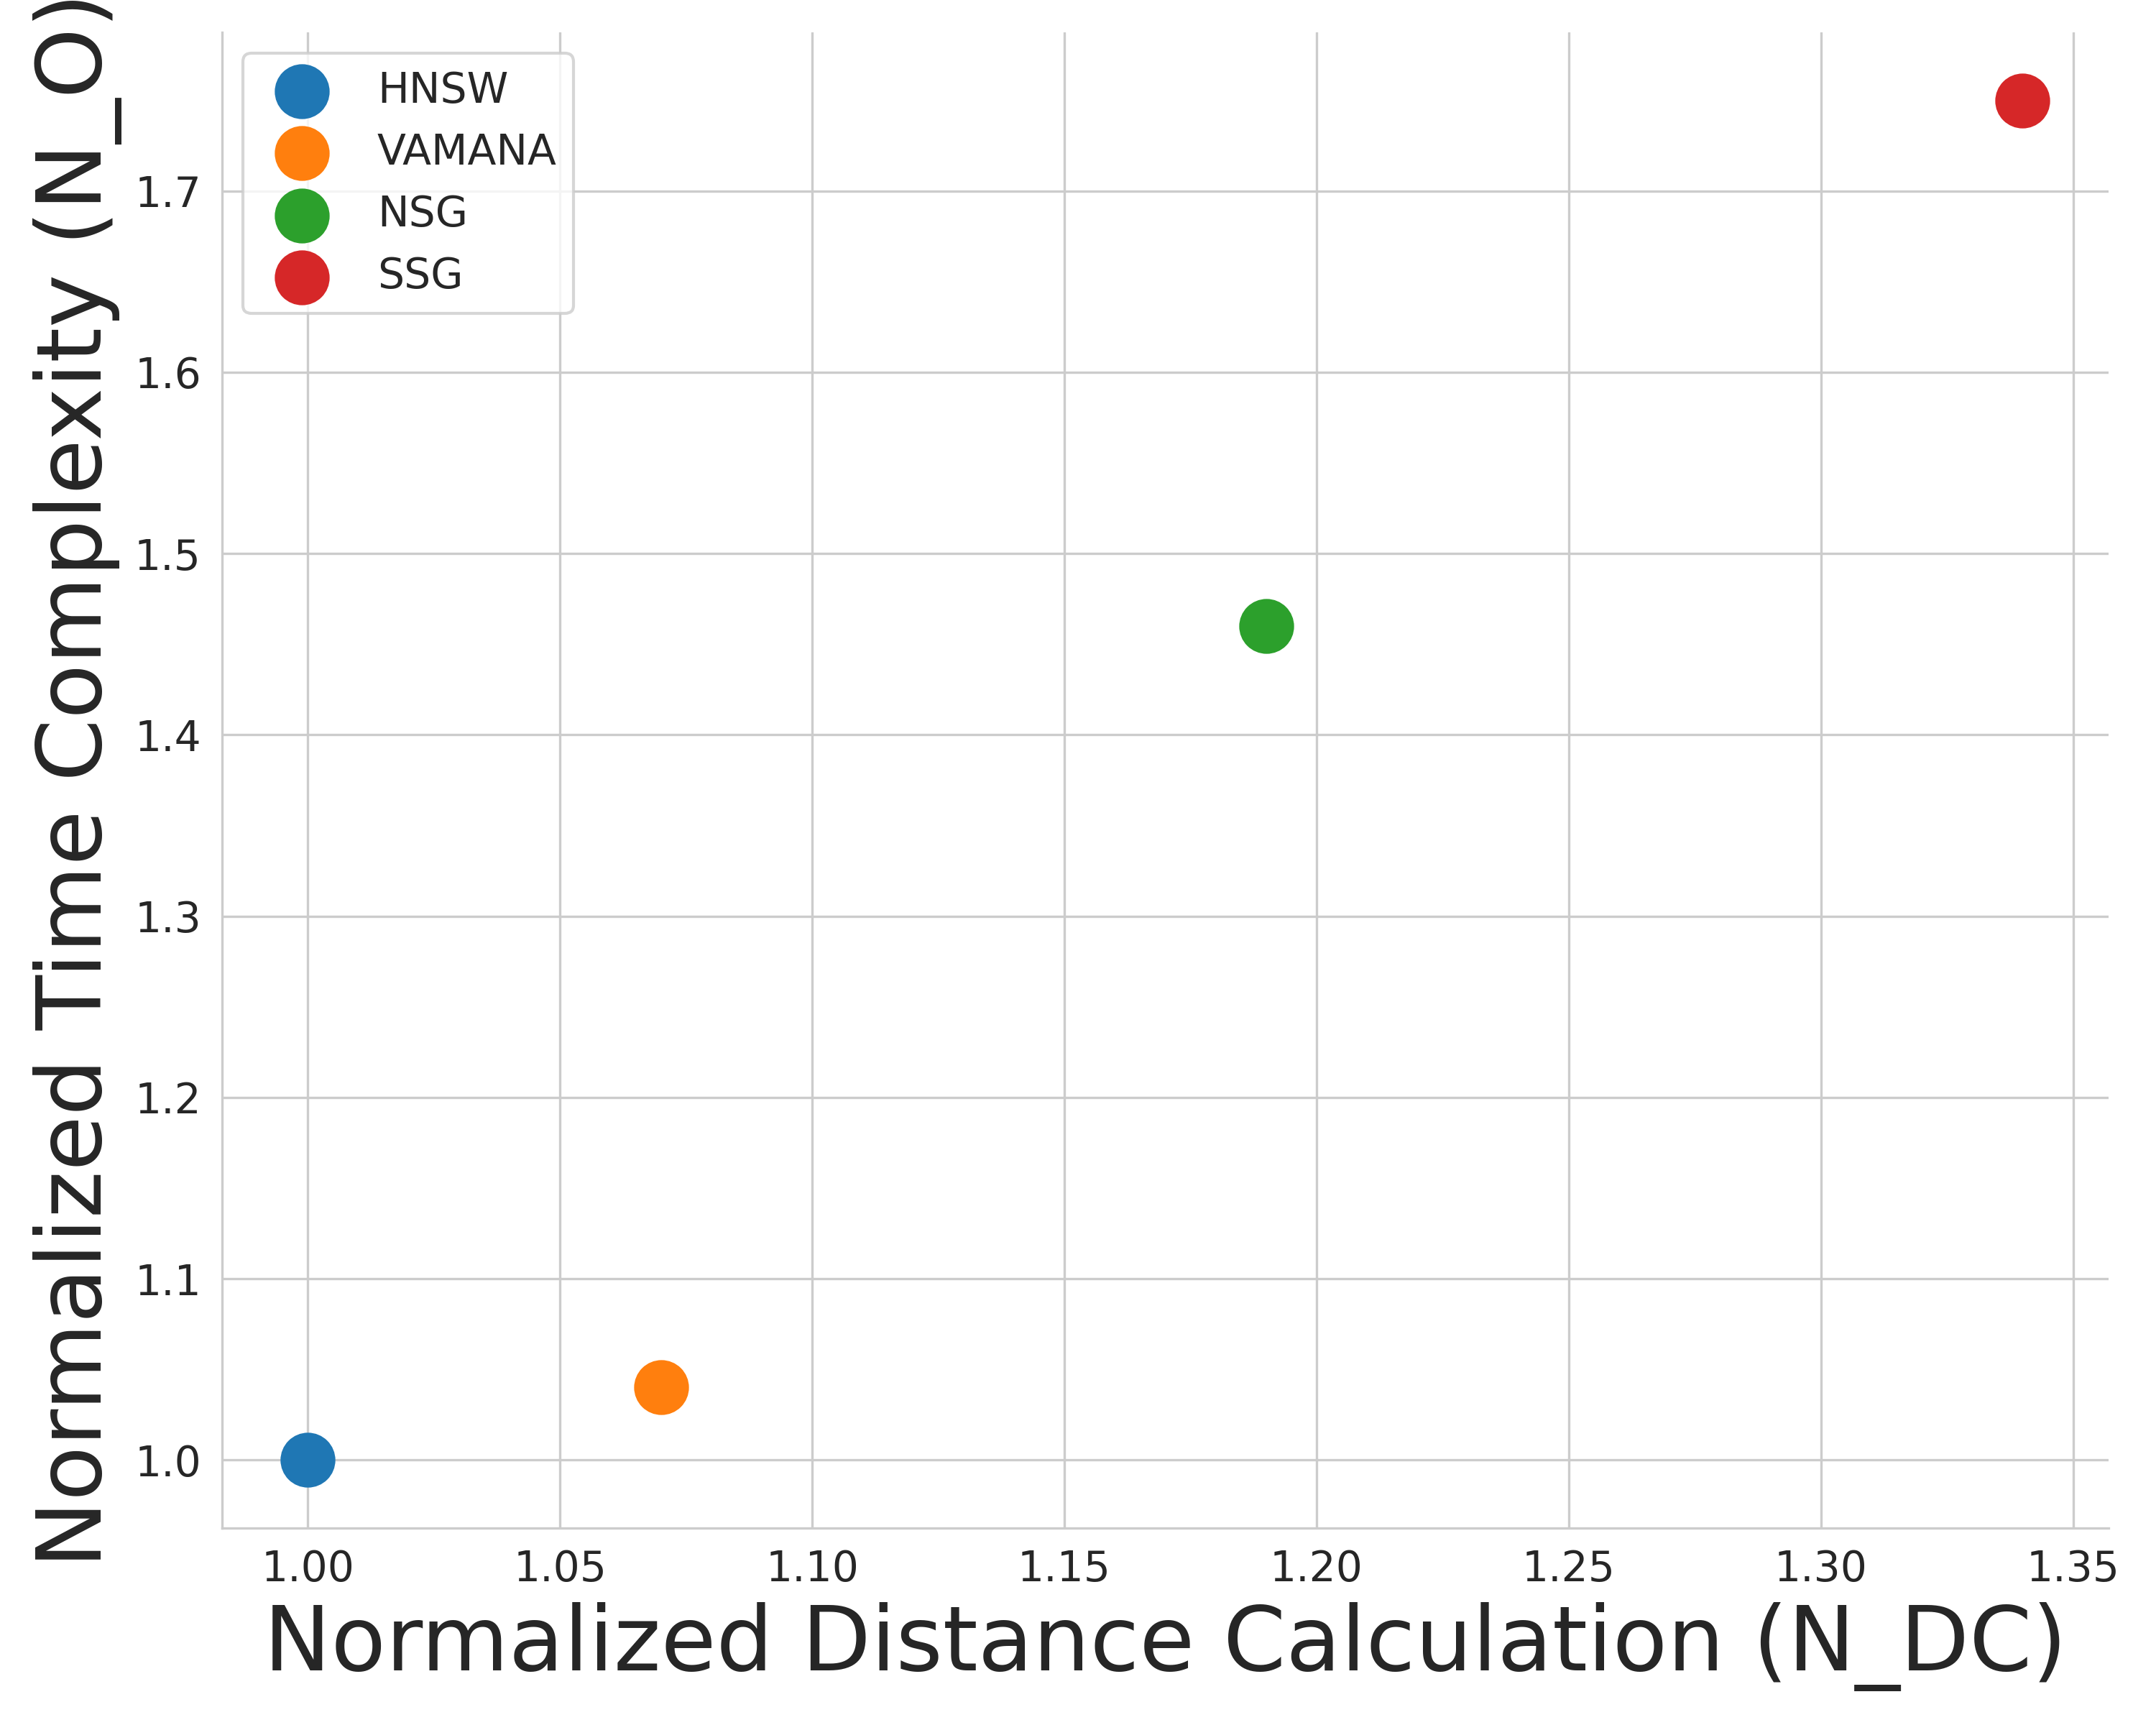
\includegraphics[width=\linewidth]{../img/Experiments/BSC/2_ndc_no.png}
  \caption{Deep2M}
  \label{fig:2_ndc_no}
\end{subfigure}
\begin{subfigure}{0.24\textwidth}
  \centering
  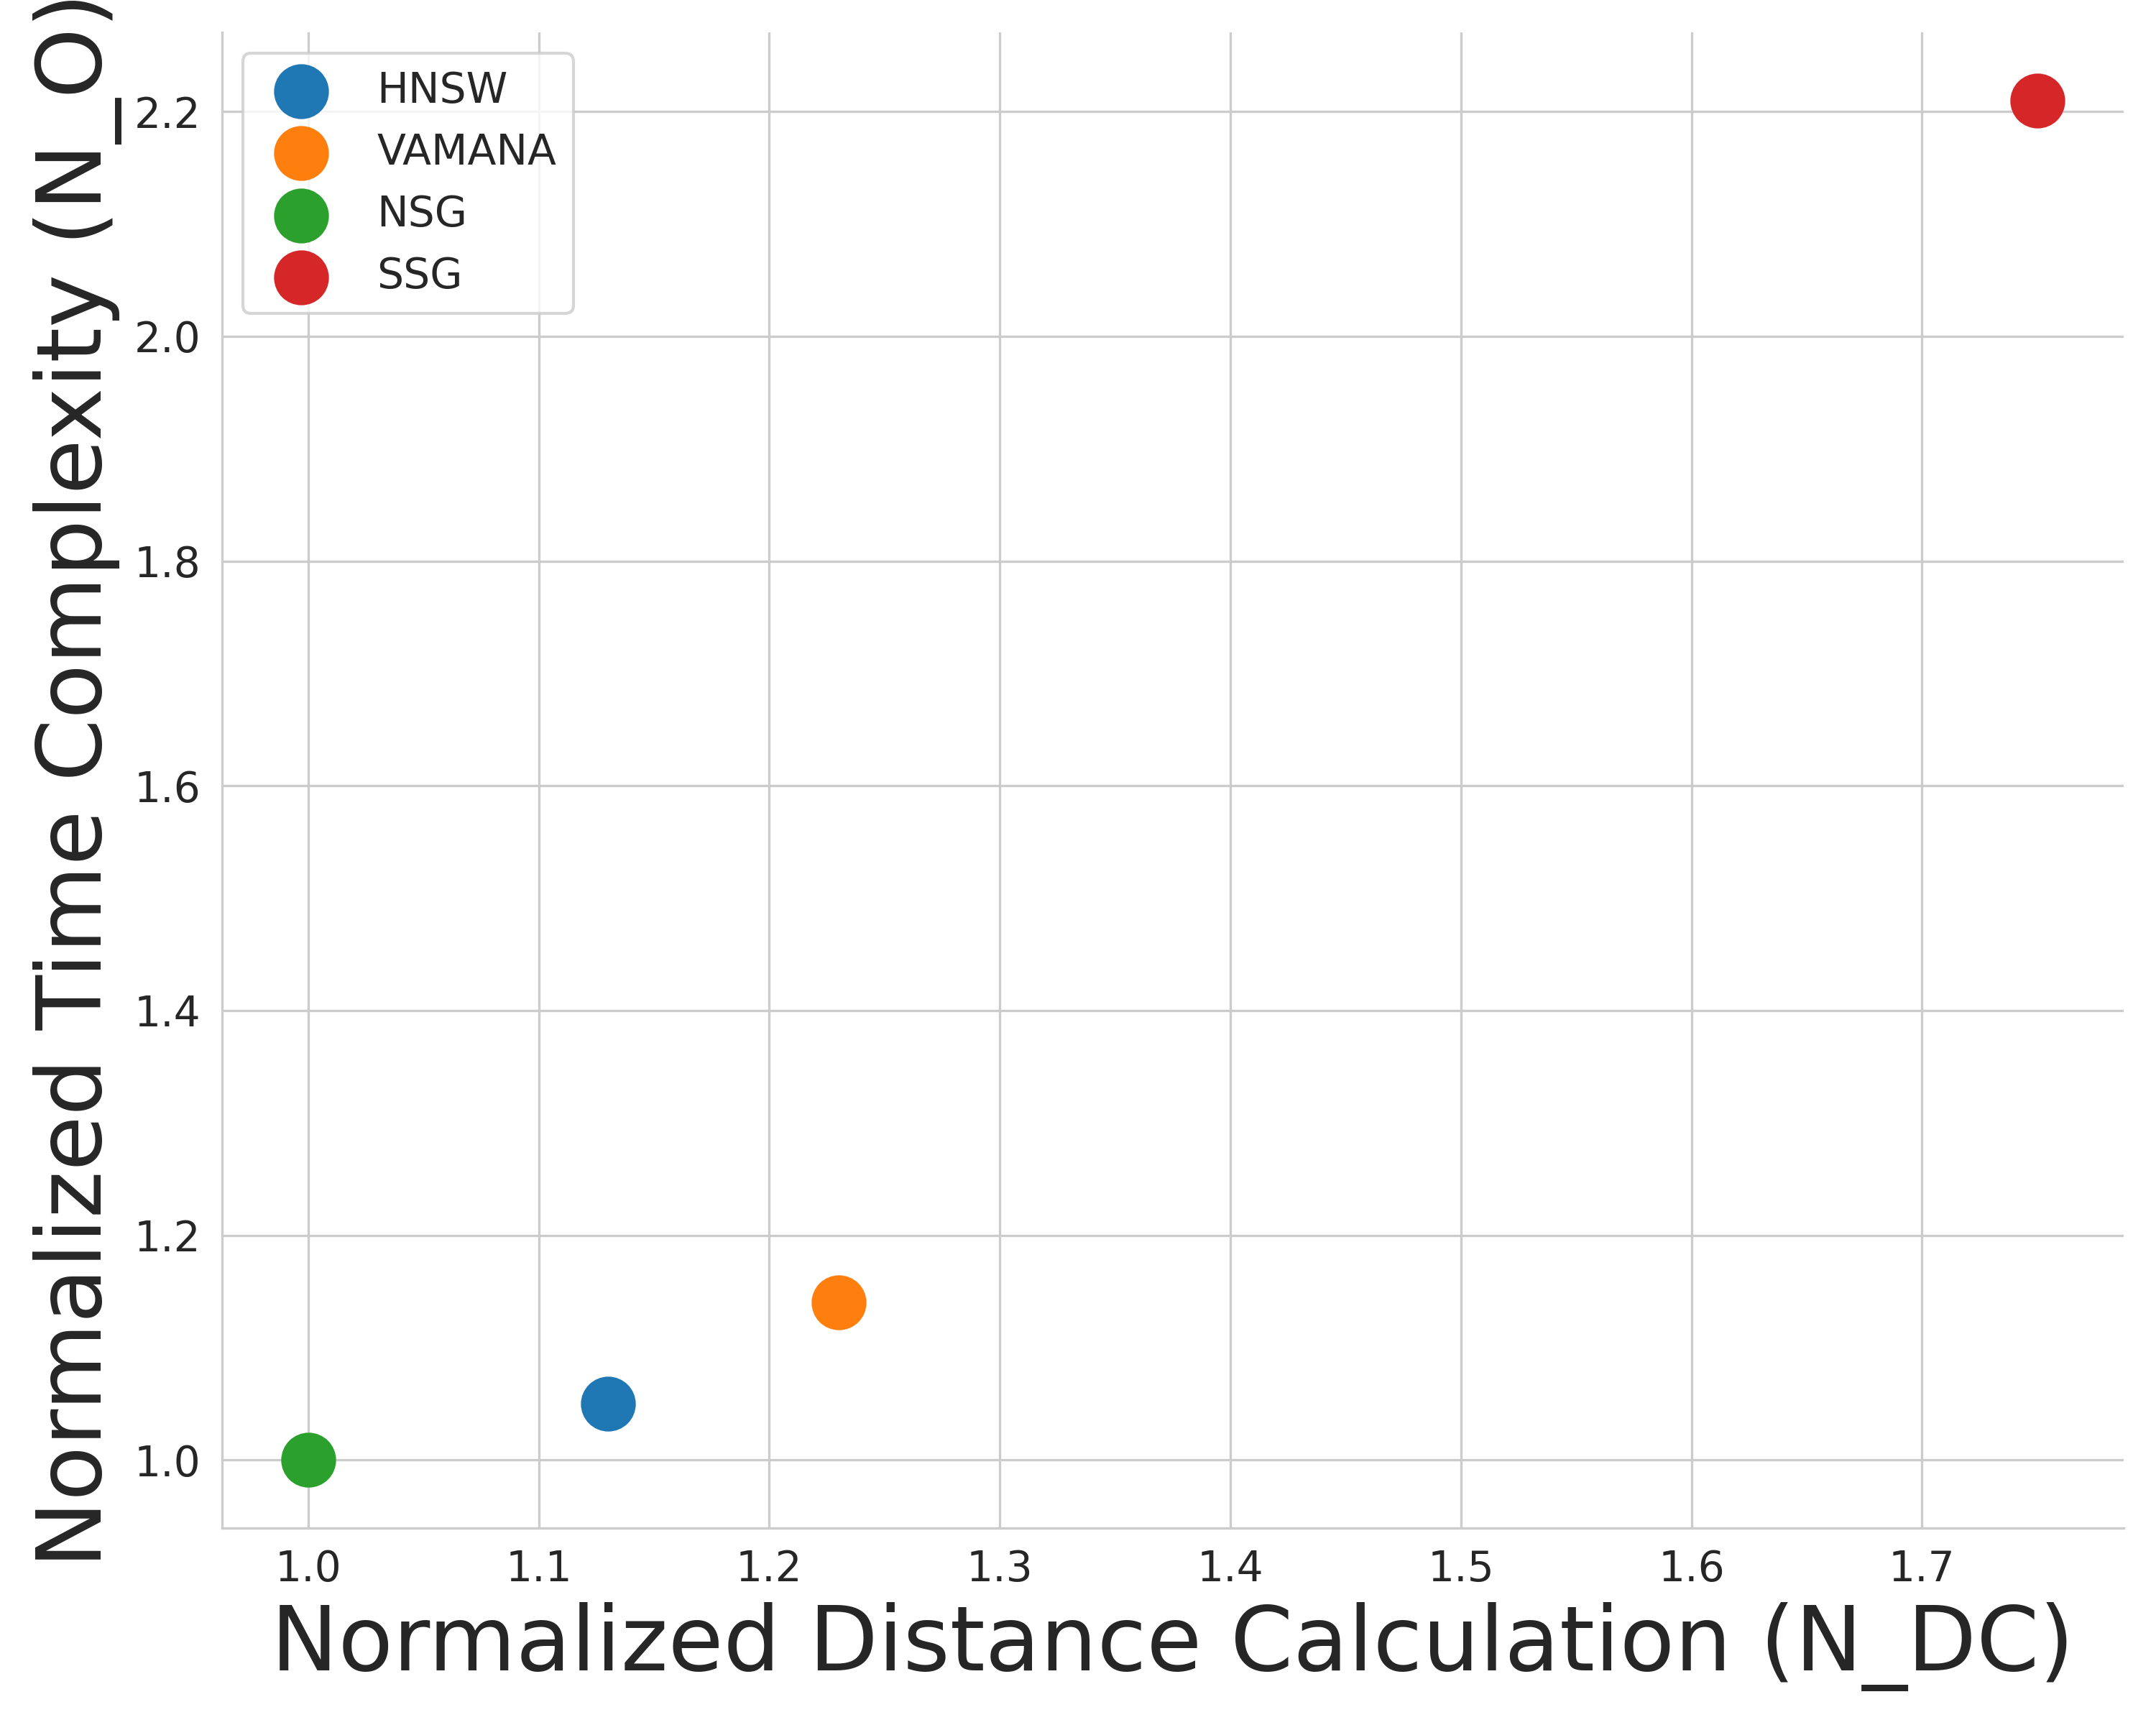
\includegraphics[width=\linewidth]{../img/Experiments/BSC/4_ndc_no.png}
  \caption{Deep4M}
  \label{fig:4_ndc_no}
\end{subfigure}
\hfill
\begin{subfigure}{0.24\textwidth}
  \centering
  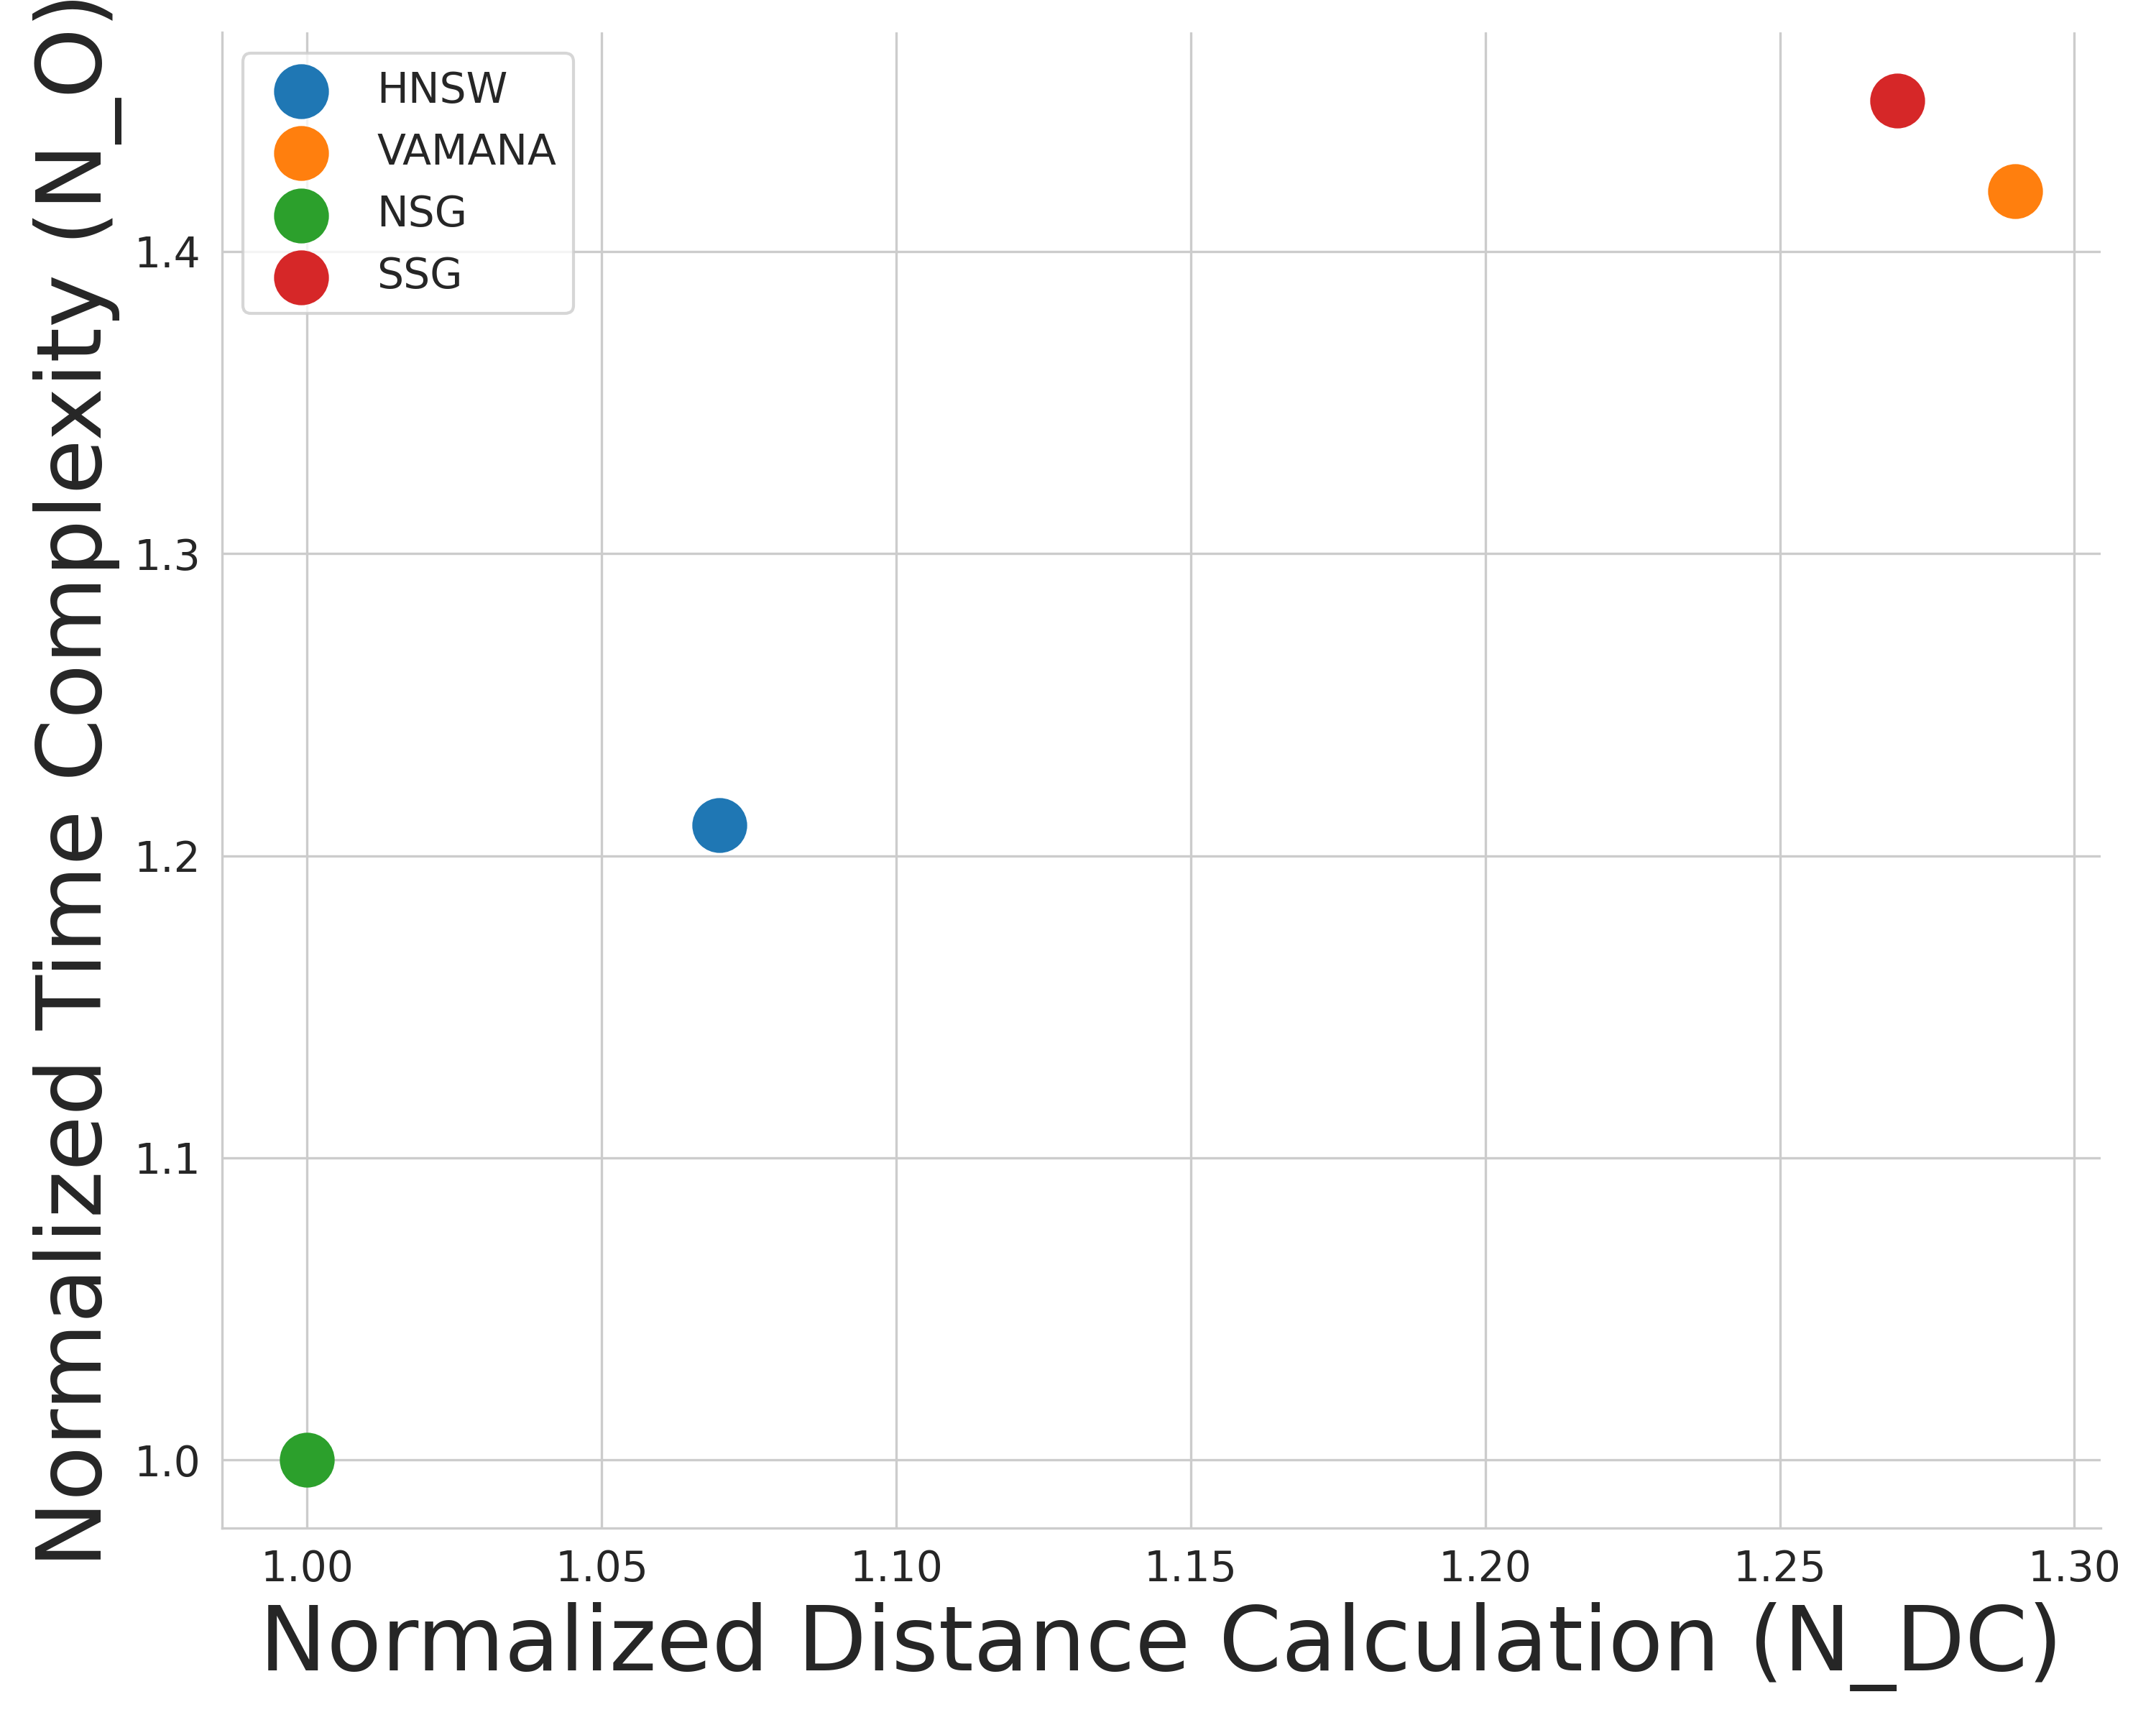
\includegraphics[width=\linewidth]{../img/Experiments/BSC/8_ndc_no.png}
  \caption{Deep8M}
  \label{fig:8_ndc_no}
\end{subfigure}
\caption{Normalized Distance Calculation (N\_DC) vs Normalized Time Complexity (N\_O) across different Deep1B dataset sizes}
\label{fig:ndc_no_plots}
\end{figure}



\end{comment}

\section{Conclusion}
In this chapter, we presented various state-of-the-art approaches for graph-based approximate vector search, along with a brief introduction to our proposed method, ELPIS. We also introduced a comprehensive taxonomy of graph-based methods, which we believe will aid the research community in understanding the key paradigms of current techniques while highlighting opportunities for further advancements in graph-based methods for vector search. 

Additionally, we provided an in-depth analysis of how Seed Selection strategies and Neighborhood Diversification (ND) methods affect graph search and indexing performance. We also explored how the theoretical complexity of the beam search algorithm translates into empirical performance during graph search. 

In the next chapter, we will delve deeper into the details of our ELPIS approach and compare its indexing and search performance with existing state-of-the-art graph methods on both real-world and synthetic datasets.


\graphicspath{{../img/graph/}}
\chapter{ELPIS: Latency-Optimized Graph-Based Vector Search}
\chaptermark{ELPIS: Latency-Optimized Graph Vector Search}
\label{chapter:elpis}

The data series community has developed tree-based similarity search techniques that outperform state-of-the-art methods on large collections of both data series and generic high-dimensional vectors, in all scenarios except for no-guarantees (\textit{ng}) approximate search, where graph-based approaches designed by the high-dimensional vector community achieve the best performance. However, building graph-based indexes is extremely expensive, both in terms of time and space.

In this chapter, we bridge these two worlds, study their corresponding solutions and performance characteristics, and propose ELPIS, a new strong baseline that leverages the best features of both to achieve superior performance in terms of indexing and \textit{ng}-approximate in-memory search. ELPIS builds the index 3x-8x faster than competitors while using 40\% less memory. It also achieves a high recall of 0.99, up to 2x faster than state-of-the-art methods, and answers 1-NN queries up to an order of magnitude faster. ELPIS is designed for latency-optimized workloads where queries are processed sequentially, not in batches, mimicking a real-world scenario where queries are unpredictable~\cite{itsawreport,DBLP:conf/edbt/GogolouTPB19,conf/sigmod/gogolou20}. This work was published in PVLDB 2023~\cite{elpis}.

\clearpage

\section{Motivation}
Vector similarity search algorithms return answers similar to a given input vector. Some algorithms provide exact results, while others return approximate answers with (\(\delta\)-\(\epsilon\)-approximate) or without (ng-approximate) guarantees on query accuracy~\cite{hydra1,hydra2}. One widely used technique is k-nearest neighbor (k-NN) search, which retrieves the top K vectors closest to a query, typically using Euclidean distance.

The data series community has developed scalable tree-based similarity search methods that outperform state-of-the-art techniques on large collections of both data series and generic high-dimensional vectors. These approaches excel in all scenarios except for \textit{ng}-approximate search, where graph-based techniques designed by the high-dimensional vector community deliver superior performance. However, building graph-based indexes on massive datasets is extremely resource-intensive, both in time and space~\cite{hydra2,neurips-2021-ann-competition,graph-survey-vldb}.

This problem is further compounded in situations with limited memory or when frequent index rebuilding is required due to updates~\cite{nsg} or evolving analytical needs (since query accuracy is influenced not only by query-time performance but also by the quality of the graph index~\cite{hydra2}), despite efforts to parallelize index construction.

To address these scalability challenges, we propose ELPIS, a solution that alleviates the bottlenecks of graph-based indexes and supports the broad range of data science applications that depend on similarity search~\cite{conf/sigmod/echihabi2020,DBLP:conf/wims/EchihabiZP20,highd-vldb-tutorial}. Instead of constructing and querying a single large graph, ELPIS employs a divide-and-conquer strategy. It splits the dataset into multiple clusters\footnote{In the context of ELPIS, the term \emph{cluster} refers to a leaf node in the ELPIS index tree, which can be interpreted as a clustering of the dataset~\cite{new-jersey-report}.} based on EAPCA summarization, and builds a graph for each cluster in parallel. During query processing, ELPIS uses the EAPCA lower-bounding distance to select an initial set of approximate answers, guiding the search and determining which clusters to search and in what order.

Both the indexing and query answering processes leverage multi-threading and SIMD instructions. During query answering, multiple threads search different clusters simultaneously. While the focus of ELPIS is on single-node systems, the concepts and lessons learned can be extended to distributed environments, where each dataset cluster can be constructed and queried on a separate node.
\section{The ELPIS approach}

We now describe ELPIS, a new baseline for graph-based similarity search that achieves better performance in both indexing and in-memory $ng$-approximate similarity search.

\subsubsection{Index Construction}

During index construction, ELPIS first splits the dataset into multiple clusters using Hercules~\cite{hercules}, where each leaf is considered a cluster, then builds graph structures in parallel on the tree's leaves. 
We opted for the state-of-the-art index tree Hercules~\cite{hercules} to cluster the dataset because it efficiently intertwines index building and data-adaptive dimensionality reduction, leading to well-clustered leaves, i.e., similar high-dimensional vectors are stored in the same leaf. 
Moreover, the Hercules tree is based on the EAPCA summarization~\cite{dstree}, 
used during search for pruning clusters. 
Any state-of-the-art graph-based similarity approach can be used within a leaf. 
We chose HNSW~\cite{hnsw}, as it led to the best overall performance (cf. Section~\ref{sec:experiments}).

Hercules builds its index tree using a double buffer to read the dataset from disk into memory in batches, while the vectors previously loaded into memory are being inserted into the tree. 
Multiple threads insert vectors in parallel into the tree. 
Each thread traverses the binary index tree to find the appropriate leaf, routing left or right depending on the split policy of the visited node. 
The resulting tree will have leaves that contain the original high-dimensional vectors and internal nodes that record statistics about the vectors belonging to their subtrees. 
Each node has its own EAPCA segmentation, and the vectors in each node are segmented using the same policy.

\begin{figure}[tb]
\captionsetup{justification=centering}	
\centering
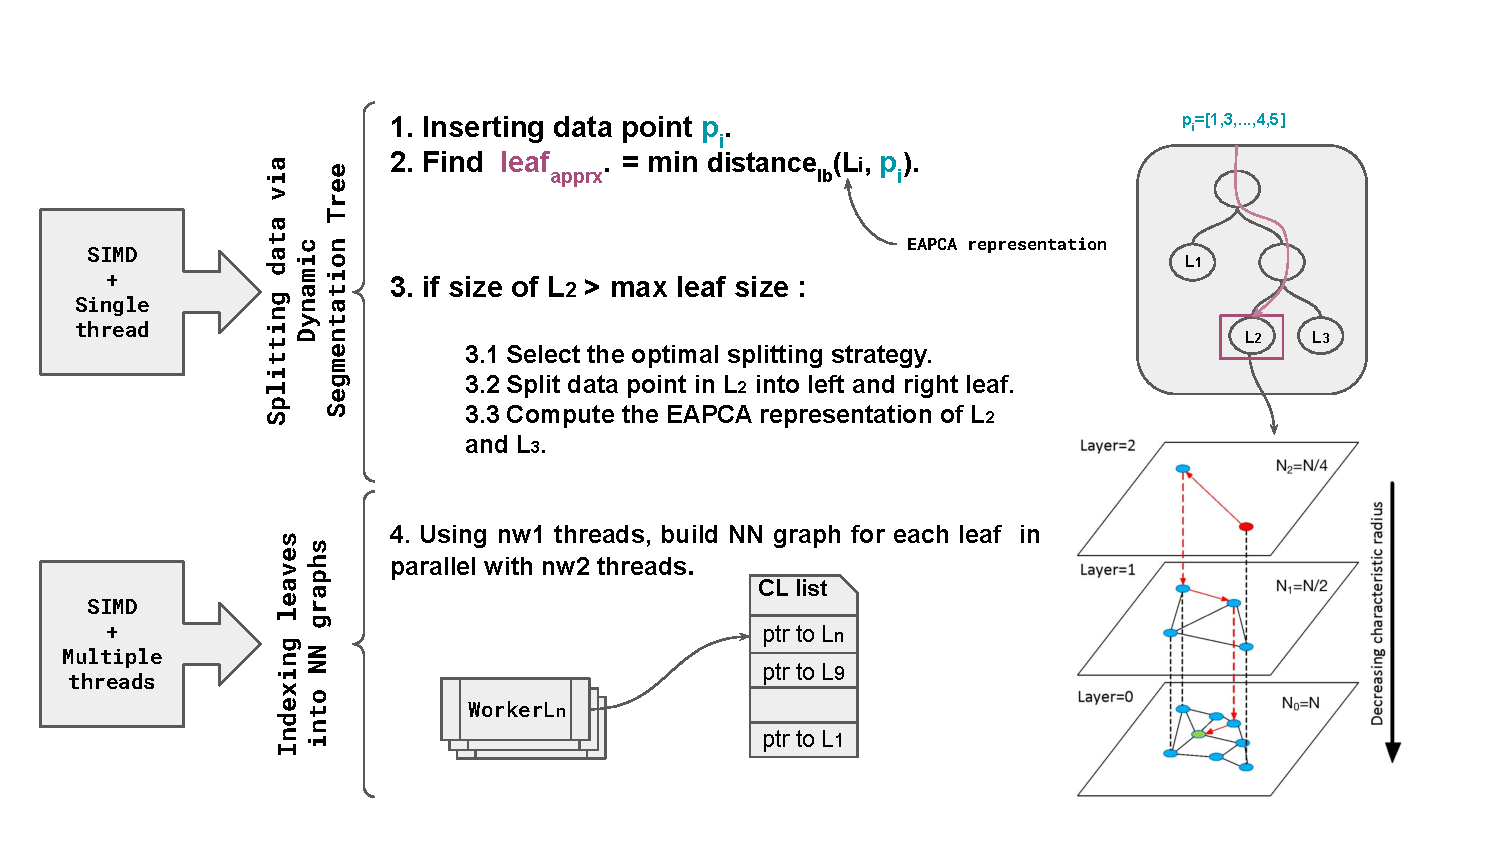
\includegraphics[width=0.90\textwidth] {../img/elpis/indexing_wf.pdf}
\caption{ELPIS Index Building Workflow}
\label{fig:hercules-index-building}
\end{figure}

ELPIS then proceeds with building an HNSW graph for each leaf in parallel. 
The main coordinator thread initializes ${n_1}$ leafCoordinator threads. 
Each leafCoordinator selects a leaf for which the graph was not built yet and creates ${n_2}$ leafWorker threads. 
Both the leafCoordinator and the leafWorkers contribute in building the graph within their corresponding leaf. 
Each one of them reads a vector from the dataset and inserts it into the graph.  
Once the graph has been built, the leafCoordinator materializes it into a separate file on disk and selects a new leaf to process. 
Index construction terminates once the graphs for all index leaves have been built.

\subsubsection{Query Answering}

Answering a query $V_Q$ with ELPIS proceeds in two major steps: (1) the Hercules tree is traversed to find $k$ initial best-so-far (bsf) neighbors to $V_Q$, which are then used to select a list of $l$ candidate leaves, i.e., clusters; and (2) a beam search is performed in parallel on the graph structures corresponding to the $l$ candidate leaves.

\begin{figure*}[tb]
\captionsetup{justification=centering}	
\begin{subfigure}{\textwidth}
\centering
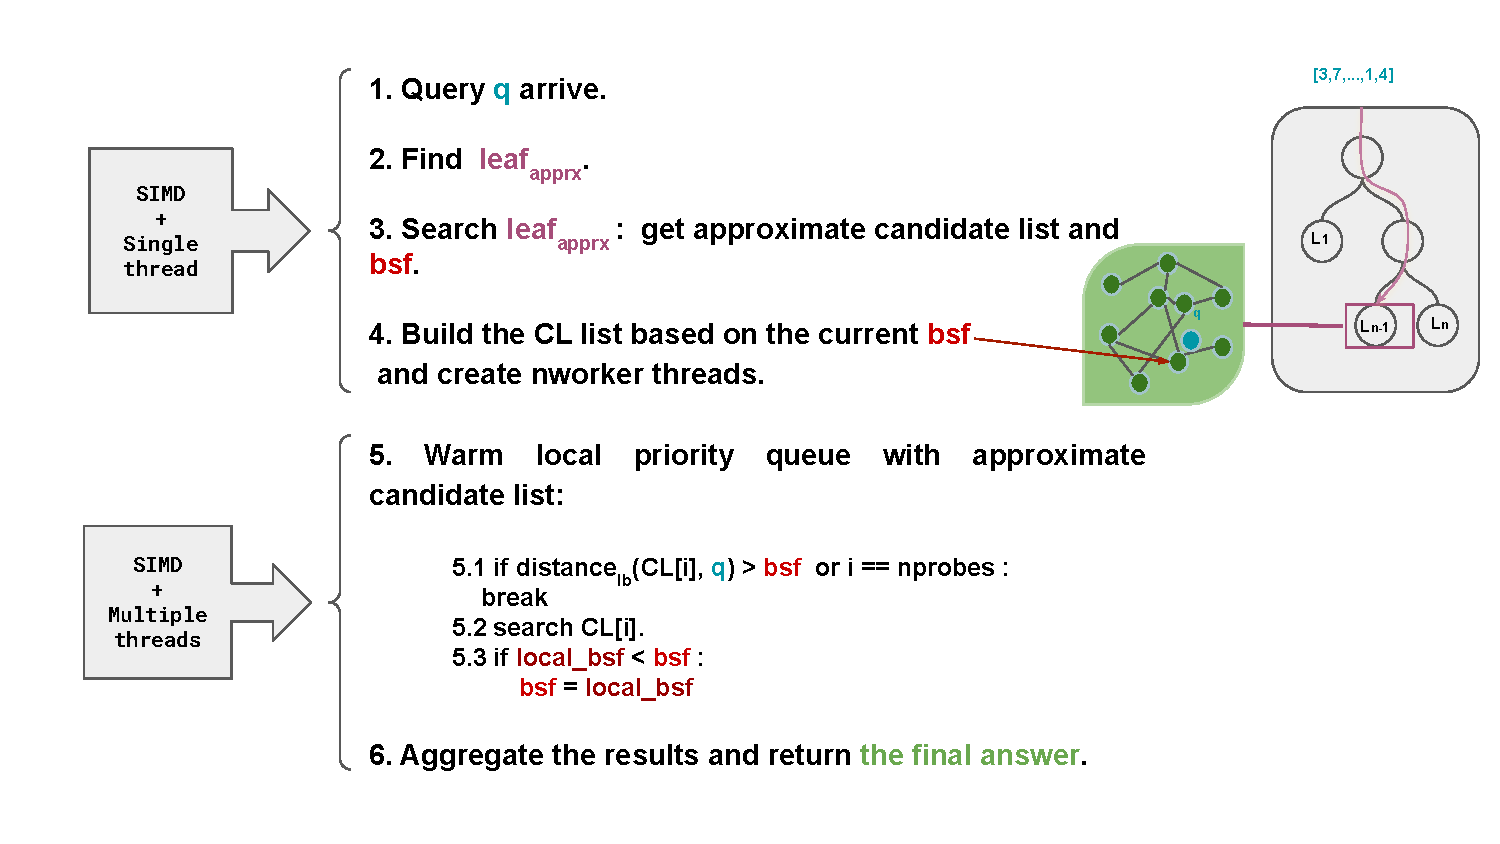
\includegraphics[width=0.90\textwidth] {../img/elpis/search_wf.pdf}
\end{subfigure}
\caption{Elpis query answering workflow}
\label{fig:Elpis-search}
\end{figure*}

During the first step, ELPIS traverses the Hercules tree, which is pre-loaded into memory, to find the leaf where $V_Q$ would have been inserted if it belonged to the dataset. Then, it performs a beam search on the HNSW graph corresponding to this leaf, returning the $k$ closest vectors to $V_Q$ as the first bsf answers. ELPIS resumes the traversal of the index tree using both the $k^{th}$ bsf answer and the EAPCA segmentation to prune nodes. The algorithm then returns, as candidate clusters, a list of $l$ leaves sorted in increasing order of their $LB_{EAPCA}$ distance to $V_Q$. 

In the second step, multiple threads process the candidate clusters in parallel, starting with the leaves that have the lowest $LB_{EAPCA}$ distances to $V_Q$. 
(Exploiting parallelism within the same graph is still an open problem and is beyond the scope of this paper, so each leaf graph is processed by only one thread, but the same thread can process multiple leaves, one at a time.) 
A thread processes a leaf by running a beam search on the corresponding HNSW graph and returning $k$ bsf answers. 
Each thread maintains a local priority queue which stores the $k$ bsf answers corresponding to the processed leaf and a local $k^{th}_{dist}$, the Euclidean distance between $V_Q$ and the $k^{th}$ bsf answer in the current leaf. 
The threads use a readers-writer lock to synchronize access to a global $k^{th}_{dist}$, the Euclidean distance between $V_Q$ and the $k^{th}$ bsf answer across all leaves. 
The global $k^{th}_{dist}$ bsf is updated every time a thread finds a better local $k^{th}_{dist}$ bsf answer. 
Once a thread finishes searching within a leaf, it uses its existing priority queue to warm up a new search on the next leaf with the lowest $LB_{EAPCA}$ to $V_Q$. 
Search terminates either after the $l$ candidate clusters are processed or once the $LB_{EAPCA}$ distances between $V_Q$ and the next leaf to be processed are larger than the $k^{th}_{dist}$. 
This is because (i) the $LB_{EAPCA}$ distance guarantees the lower-bounding property, i.e., the Euclidean distance between any two points in the original high-dimensional space is guaranteed to be larger than or equal to their $LB_{EAPCA}$ distance; and (ii) the list of candidate leaves is sorted in increasing order of $LB_{EAPCA}$. 
Once all threads terminate, ELPIS computes the final results: it aggregates the answers from all local priority queues and selects the $k$ answers with the smallest Euclidean distance to $V_Q$.

\section{Experimental Evaluation}
\label{sec:experiments}

In this section, we conduct a comprehensive experimental evaluation of ten state-of-the-art graph-based vector search methods, including ELPIS. We assess the indexing and query-answering performance of these methods on a variety of real and synthetic datasets. All artifacts are available in~\cite{url/GASS}.

\subsection{Framework}
\noindent{\bf Setup.} 
Methods were compiled with GCC 8.2.0 under Ubuntu Linux 20.04 (Rocky Linux 8.5 on HPC) using default compilation flags and optimization level 3. Experiments were conducted on an Intel Xeon Platinum 8276 server with 4 sockets, each with 28 cores and 1 thread per core.
The CPU cache configuration is: 32KB L1d, 32KB L1i, 1,024KB L2, and 39,424KB L3 cache. The server includes a 1.5TB RAM via 24x 64GiB DDR4 DIMMs.}

\noindent{\bf Algorithms.} We cover the following methods: ELPIS~\cite{elpis}, HNSW~\cite{hnsw}, NSG~\cite{nsg}, Vamana~\cite{vamana}, EFANNA~\cite{efanna}, HCNNG~\cite{hcnng}, DPG~\cite{dpg}, KGraph~\cite{kgraph}, NGT~\cite{ngt_library}, DPG~\cite{dpg}, and two versions of SPTAG~\cite{SPTAG4} (SPTAG-BKT and SPTAG-KDT, using BKT and K-D Trees, respectively). We also included LSHAPG~\cite{lshapg}, new technique not evaluated in the latest survey~\cite{graph-survey-vldb}. IEH~\cite{ieh} and FANNG~\cite{fanng} are excluded due to suboptimal performance~\cite{graph-survey-vldb, nsg}, and HVS~\cite{hvs} due to difficulties running the official implementation~\cite{hvsgithub}. We use the most efficient publicly available C/C++ implementations for each algorithm, leveraging multi-threading and SIMD vectorization to optimize performance.  We also carefully inspected all code bases and, as is common in the literature ~\cite{graph-survey-vldb, diskanncode, nsgcode,ssgcode,ngtcode,sptagcode}, disabled the optimizations that would lead to an unfair evaluation such as cache pre-warming in Vamana and L2-normalized Euclidean distance in NSG, EFANNA, and Vamana. Since all methods except ELPIS and HNSW use a single linear buffer as a priority queue, we modified the original implementations of these two algorithms (which used two max-heap priority queues)~\cite{url/Elpis,url/hnsw}. The modifications to each code base are documented in~\cite{url/GASS}. All algorithms were tuned to achieve a good accuracy/efficiency trade-off (Please refer to Appendix~\ref{appendix:parameters} for more details on the parameters tuning and choice) . 

\noindent{\bf Datasets.} 
We use seven real-world datasets from various domains, including deep network embeddings, computer vision, neuroscience, and seismology:  
(i) \emph{Deep}~\cite{url/data/deep1b} contains 1 billion 96-dimensional vectors extracted from the final layers of a convolutional neural network;  
(ii) \emph{Sift}~\cite{conf/icassp/jegou2011,url/data/sift} consists of 1 billion 128-dimensional SIFT vectors representing image feature descriptors;  
(iii) \emph{SALD}~\cite{url/data/eeg} provides neuroscience MRI data with 200 million 128-dimensional data series;  
(iv) \emph{Seismic}~\cite{url/data/seismic} contains 100 million 256-dimensional time series representing earthquake recordings from seismic stations worldwide;  
(v) \emph{Text-to-Image}~\cite{url/data/text2image} offers 1 billion 200-dimensional image embeddings from Se-ResNext-101 along with 50 million DSSM-embedded text queries for cross-modal retrieval under domain shifts;  
(vi) \emph{GIST}~\cite{gist} contains 1 million 960-dimensional vectors, using GIST descriptors~\cite{gistdesc} to capture spatial structure and color layout of images;  and
(vii) \emph{ImageNet1M}, a new dataset that we generated from the original ImageNet~\cite{imagenet}, producing embeddings of 1 million original vectors using the ResNet50 model~\cite{resnet}, with PCA applied to reduce dimensionality to 256. We select subsets of different sizes from the Sift, Deep, SALD and Seismic datasets, and we refer to each subset with the name of the dataset followed by the subset size in GBs (e.g., Deep25GB). 
We refer to the 1-million and 1-billion datasets with the 1M and 1B prefixes, respectively. 
To evaluate the methods on datasets with different distributions, we generate three random 25GB datasets RandPow0, % (uniform distribution~\cite{url/Elpis}), 
RandPow5 and RandPow50, each with 256 dimensions, following the power law distribution~\cite{powerlaw} using three power law exponents: 0 (uniform~\cite{url/power-law}), 5 and 50 (very skewed).
The power law distribution models many real world phenomena (including in economics, physics, biology, social networks, etc.). 
It is a relationship of type $Y= kX^a$, where $Y$ and $X$ are variables of interest, $a$ is the power law exponent and $k$ is a constant. 
The skewness of a dataset distribution increases with $a$. 
When $a = 0$, the dataset is evenly distributed.

\noindent{\bf Dataset Complexity.}
The complexity of the datasets in our experimental evaluation is assessed using Local Intrinsic Dimensionality (LID)~\cite{lid15,DBLP:journals/is/AumullerC21} and Local Relative Contrast (LRC)~\cite{rc,DBLP:journals/is/AumullerC21}. 
The LID and LRC for a query point \( x \) are defined as follows:

\noindent{\textbf{Local Intrinsic Dimensionality (LID)}} The LID of a query point \( x \) provides a local estimate of the dimensionality around \( x \) based on the distances to its nearest neighbors. Formally, LID is defined as:

\begin{equation}
    \text{LID}(x) = -\left(\frac{1}{k} \sum_{i=1}^{k} \log \frac{\text{dist}_i(x)}{\text{dist}_k(x)}\right)^{-1}
    \label{eq:lid}
\end{equation}

Where:
\begin{itemize}
    \item \( x \) is the query point.
    \item \( \text{dist}_i(x) \) is the distance from \( x \) to its \( i \)-th nearest neighbor.
    \item \( \text{dist}_k(x) \) is the distance from \( x \) to its \( k \)-th nearest neighbor.
    \item \( k \) is the number of nearest neighbors considered.
\end{itemize}

\noindent{\textbf{Local Relative Contrast (LRC)}} The LRC metric quantifies the contrast between the mean distance to the neighbors of a query point and the distance to the \( k \)-th nearest neighbor. LRC is defined as:

\begin{equation}
    \text{LRC}(x) = \frac{\text{dist}_{\text{mean}}(x)}{\text{dist}_k(x)}
    \label{eq:lrc}
\end{equation}

Where:
\begin{itemize}
    \item \( \text{dist}_{\text{mean}}(x) \) is the mean distance from \( x \) to its \( k \)-nearest neighbors.
    \item \( \text{dist}_k(x) \) is the distance from \( x \) to its \( k \)-th nearest neighbor.
\end{itemize}

Figure~\ref{fig:datacomp:rc} presents the boxplot results for RC and LID values, calculated with a subset of one million data points randomly sampled from each dataset and a $k$ equals to 100. On the y-axis, we have the LID or LRC values, providing a measure of dataset complexity, while the x-axis enumerates the names of the datasets under investigation. High LRC in a dataset corresponds to distinctive data points, potentially marking boundaries or outliers, which could influence the stability and accuracy of k-NN results, whereas low LRC indicates homogeneous regions, leading to more consistent k-NN outcomes. 
High LID reveals complex, high-dimensional local structures, possibly complicating k-NN searches due to the “curse of dimensionality,” while low LID indicates simpler, low-dimensional areas, enhancing the efficiency and precision of k-NN searches. 
LID represents the intrinsic dimensionality of the data (and can be significantly lower than the original dimensionality of the data space): the lower the LID, the easier the search is.

\begin{figure}[tb]
    \centering
    \begin{subfigure}{0.48\columnwidth}
    \centering
			\captionsetup{justification=centering}	
        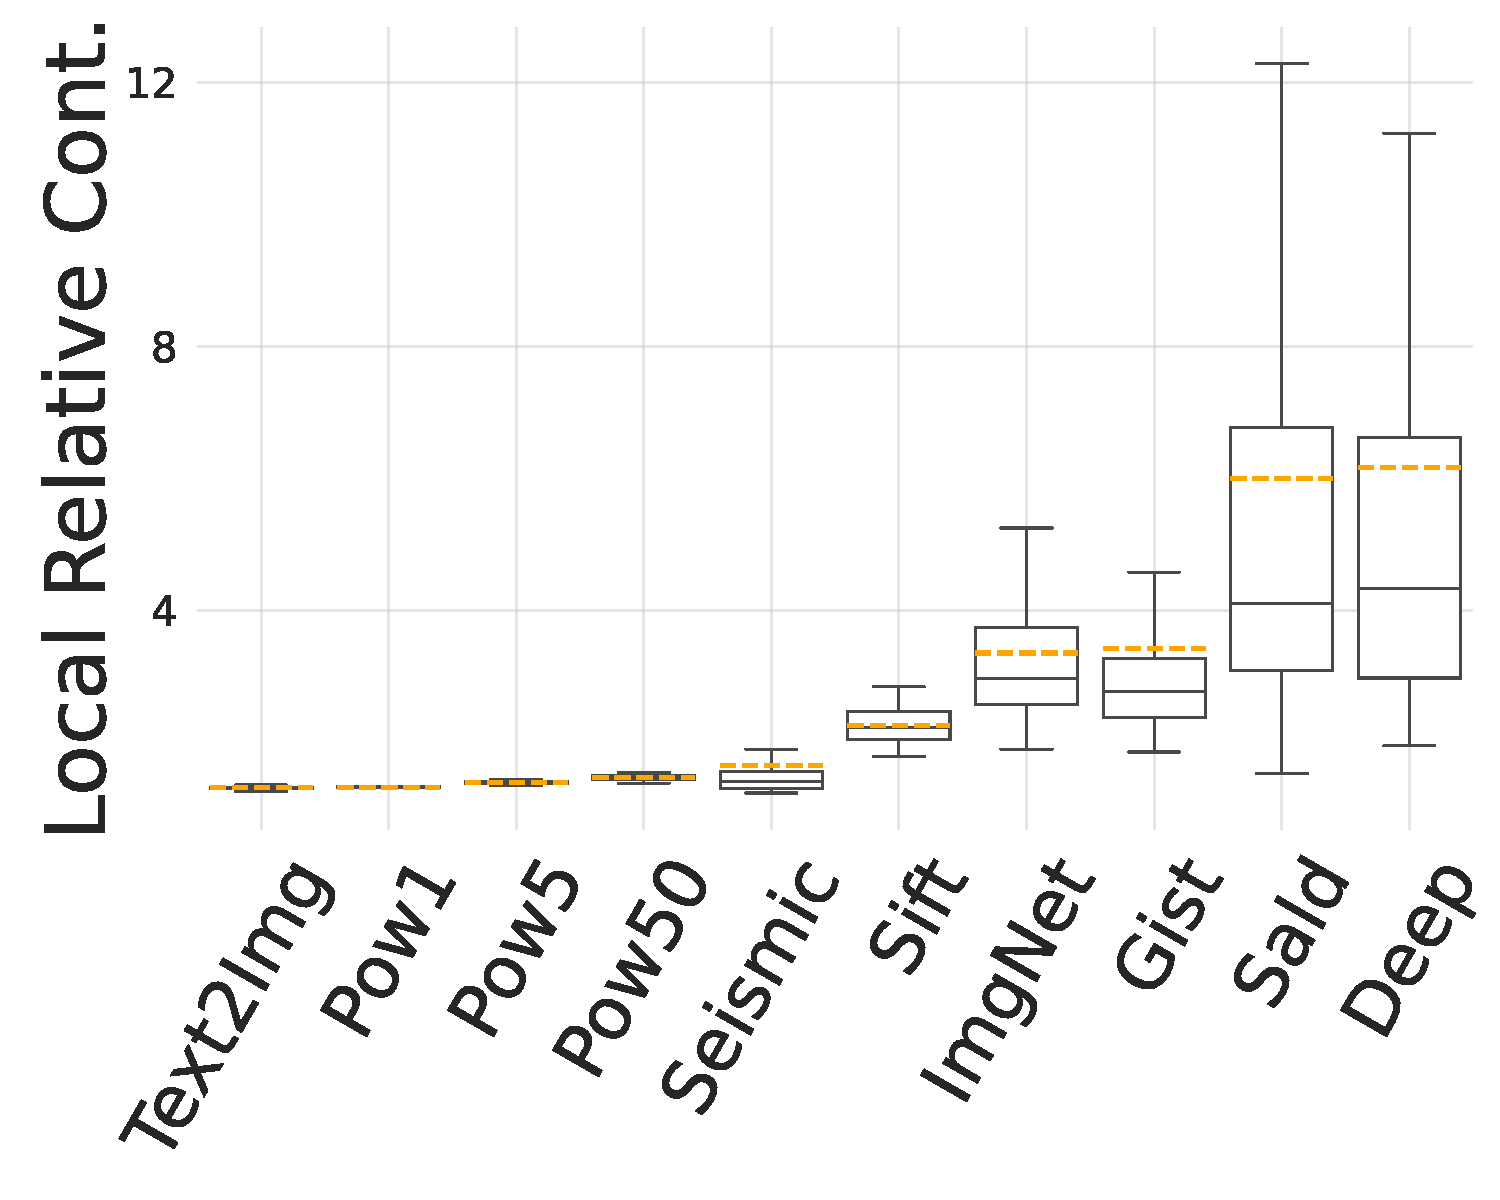
\includegraphics[width=\columnwidth]{../img/Experiments/data/query_rc_plot.pdf}
        \caption{Local Relative Contrast}
        \label{fig:datacomp:rc}
    \end{subfigure}
    \begin{subfigure}{0.499\columnwidth}
    \centering
			\captionsetup{justification=centering}	
        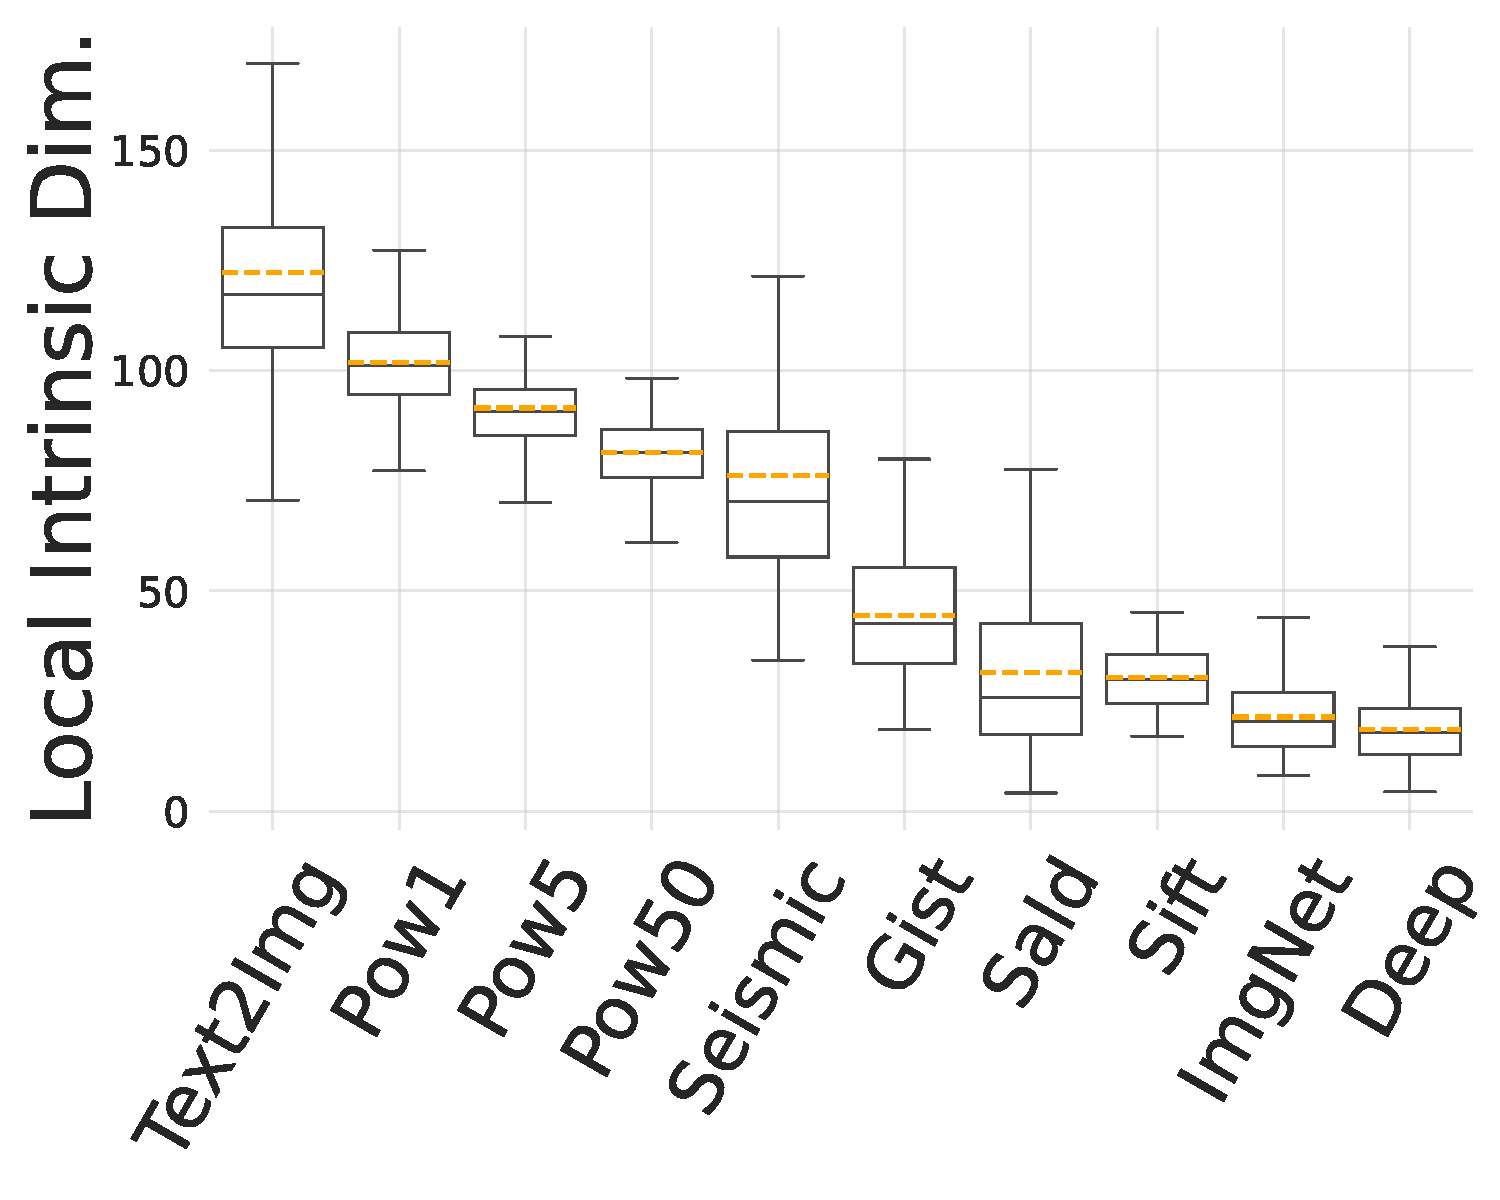
\includegraphics[width=\columnwidth]{../img/Experiments/data/query_lid_plot.pdf}
        \caption{Local Intrinsic Dimensionality}
        \label{fig:datacomp:lid}
    \end{subfigure}
    \caption{Dataset complexity}
    \label{fig:datacomp}
\end{figure}

Note that the orange horizontal line in Figure~\ref{fig:datacomp:rc} denotes the mean LRC, which corresponds to the Relative Contrast (RC)~\cite{DBLP:journals/is/AumullerC21} of the dataset. The Pow0, Pow5, Pow50, and Seismic datasets have the highest LID and lowest LRC values, indicating that they are challenging datasets for vector search~\cite{DBLP:journals/is/AumullerC21}.

The random datasets we generated are highly clustered and high-dimensional, reflecting the same difficulties for k-NN methods as the Text-to-image and Seismic datasets, and to a lesser extent, the SALD dataset. Meanwhile, Imagenet, Sift and Deep are the easiest datasets in our workload to query, with the lowest LID and highest LRC values. In the results section, we will remark how graph-based ng-approximate similarity search methods face high difficulties in achieving high accuracy for query answering in datasets with high LID and low LRC, and perform well when dealing with low LID and high LRC datasets.

\noindent{\bf Queries.}  Query sets include 100 vectors processed sequentially, not in batches, mimicking a real-world scenario where queries are unpredictable~\cite{itsawreport,DBLP:conf/edbt/GogolouTPB19,conf/sigmod/gogolou20}. Results with 1 million queries are extrapolated from 100 query sets. For Deep, Sift, GIST, and Text-to-Image, queries are randomly sampled from available query workloads. For SALD, ImageNet, and Seismic, 100 queries are randomly selected from the datasets and excluded from the index-building phase.
For hardness experiments, we use Deep query vectors of varying complexity, denoted as a percentage ranging from 1\% to 10\%. These vectors were obtained by adding Gaussian noise (\(\mu = 0\), \(\sigma^2\) ranging from 0.01 to 0.1) to randomly choose dataset vectors, with the percentage reflecting the \(\sigma^2\) value~\cite{johannesjoural2018}.
The 100-query workloads for the power law distribution datasets are generated following the same distributions using different seeds. % as its respective dataset. 
Unless otherwise stated, all experiments were conducted with 10-NN queries per the standard in the community~\cite{neurips-2021-ann-competition,url/Elpis,ann-benchmark-journal}.
We use 100-NN queries to evaluate dataset complexity because a higher k improves the estimation of LID and LRC (Eqs. 5.1-5.2).
\\
\noindent{\textbf{Accuracy Measures}} The accuracy of a $k$-NN query \( S_Q \) is evaluated using the \textit{Recall} metric~\cite{Recall}. Recall measures the proportion of true nearest neighbors that are correctly returned by the query. It is formally defined as:

\begin{equation}
    \text{Recall}(S_Q) = \frac{\# \text{true neighbors returned by } Q}{k}
    \label{eq:recall}
\end{equation}

Where:
\begin{itemize}
    \item \( S_Q \) is the set of neighbors returned by the query \( Q \).
    \item \( k \) is the number of true nearest neighbors.
\end{itemize}

The reported recall represents the average recall across all queries in the query workload.



\subsubsection{Choosing the Clustering Technique} 


\begin{figure}[tb] 
	\captionsetup{justification=centering}
	\centering
	\begin{subfigure}{\columnwidth}
 \centering
		
\includegraphics[width=0.7\columnwidth]{../img/elpis/ElpisvsKmeans/legend.pdf}
	\end{subfigure}	
	\begin{subfigure}{\sfig\columnwidth}
		\captionsetup{justification=centering}
		\centering
		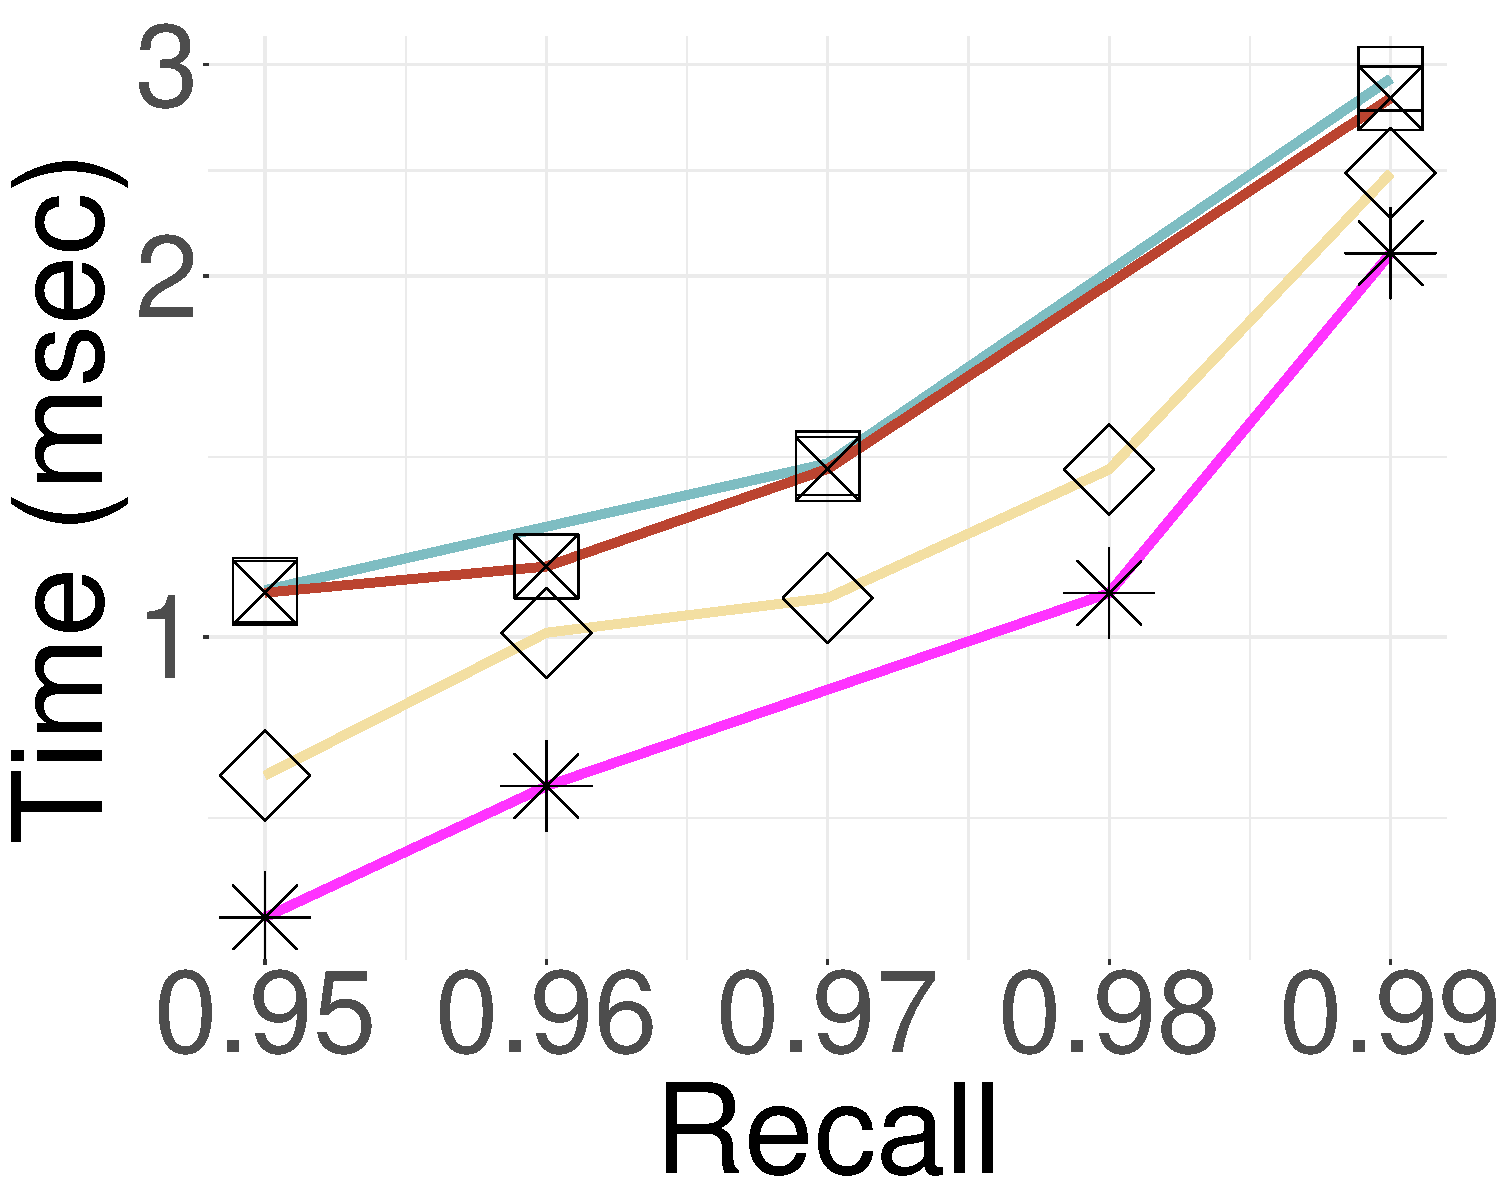
\includegraphics[width=\columnwidth]{../img/elpis/ElpisvsKmeans/qrstime.pdf}      
		\caption{Avg. query time} 
		\label{fig:elpis_kmeans:proc}
	\end{subfigure}	
 \hspace{0.4cm}
	\begin{subfigure}{\sfig\columnwidth}
		\captionsetup{justification=centering}
		\centering
		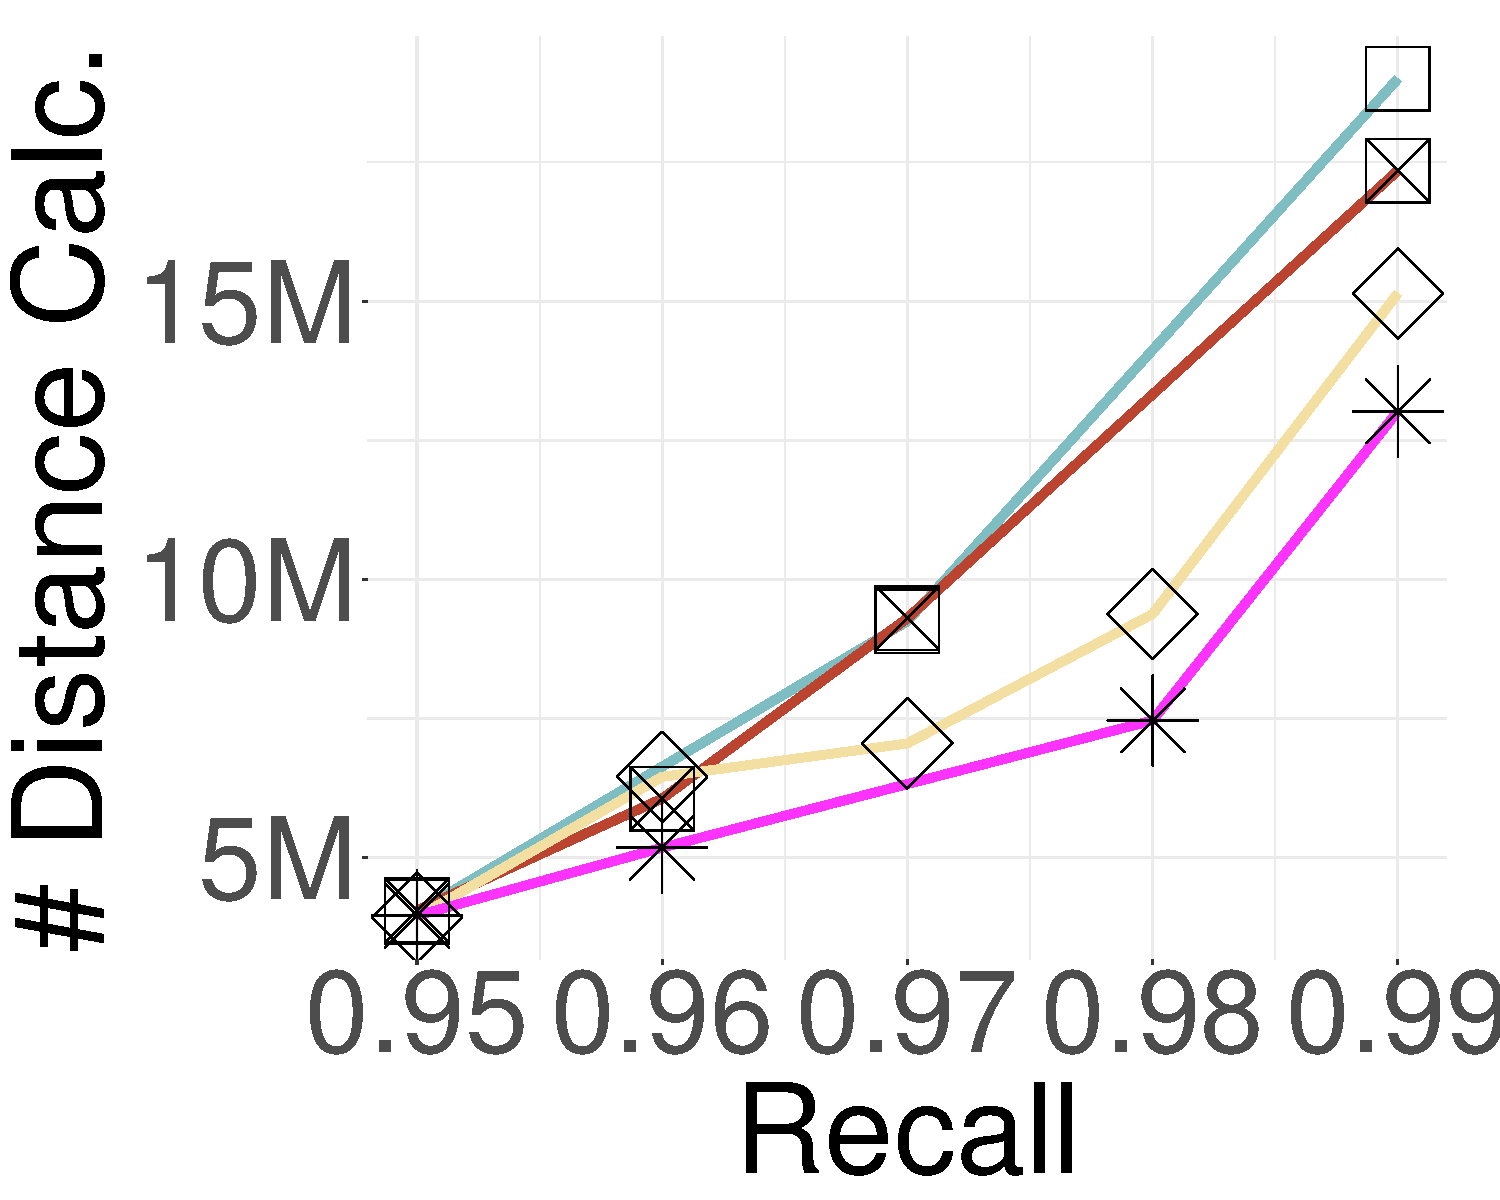
\includegraphics[width=\columnwidth]{../img/elpis/ElpisvsKmeans/qrsdc.pdf}                                                        
		\caption{Num. Dcs} 
		\label{fig:elpis_kmeans:distances}
	\end{subfigure}		


	\begin{subfigure}{\sfig\columnwidth}
		\captionsetup{justification=centering}
		\centering
		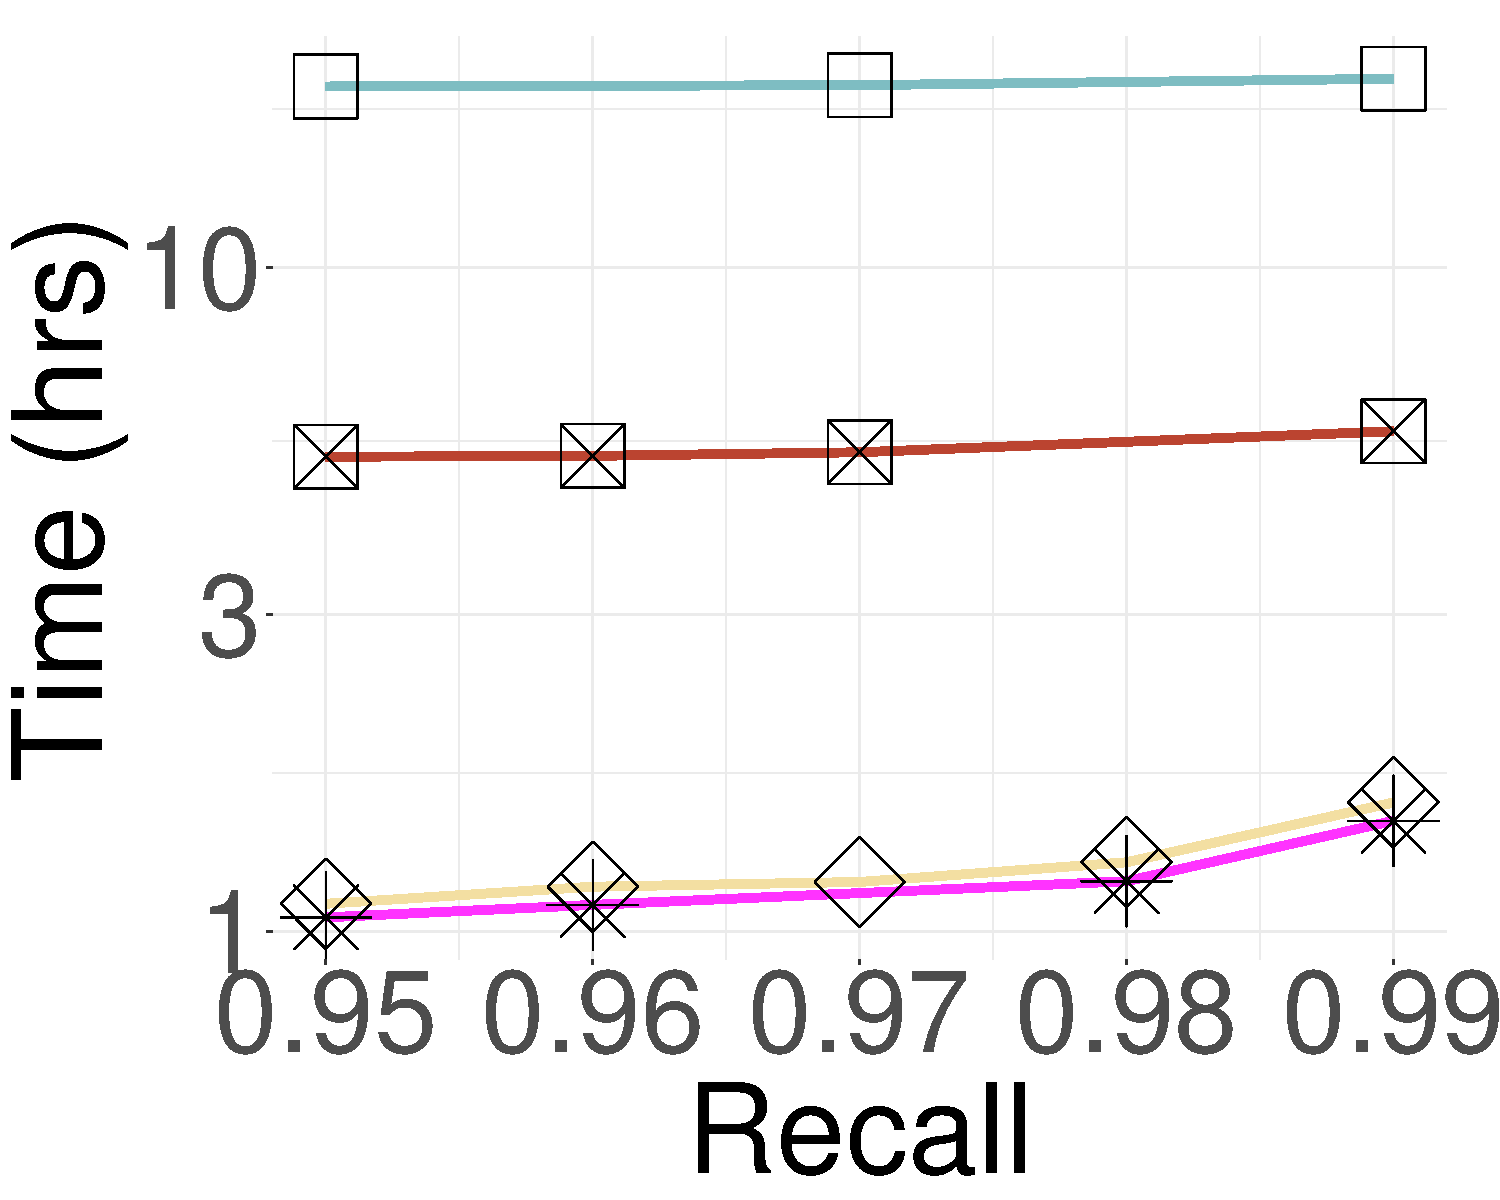
\includegraphics[width=\columnwidth]{../img/elpis/ElpisvsKmeans/idxqrs.pdf}                                             \caption{Idx+1M queries} 
		\label{fig:elpis_kmeans:idxproc}
	\end{subfigure}
  \hspace{0.4cm}
	\begin{subfigure}{\sfig\columnwidth}
		\captionsetup{justification=centering}
		\centering
		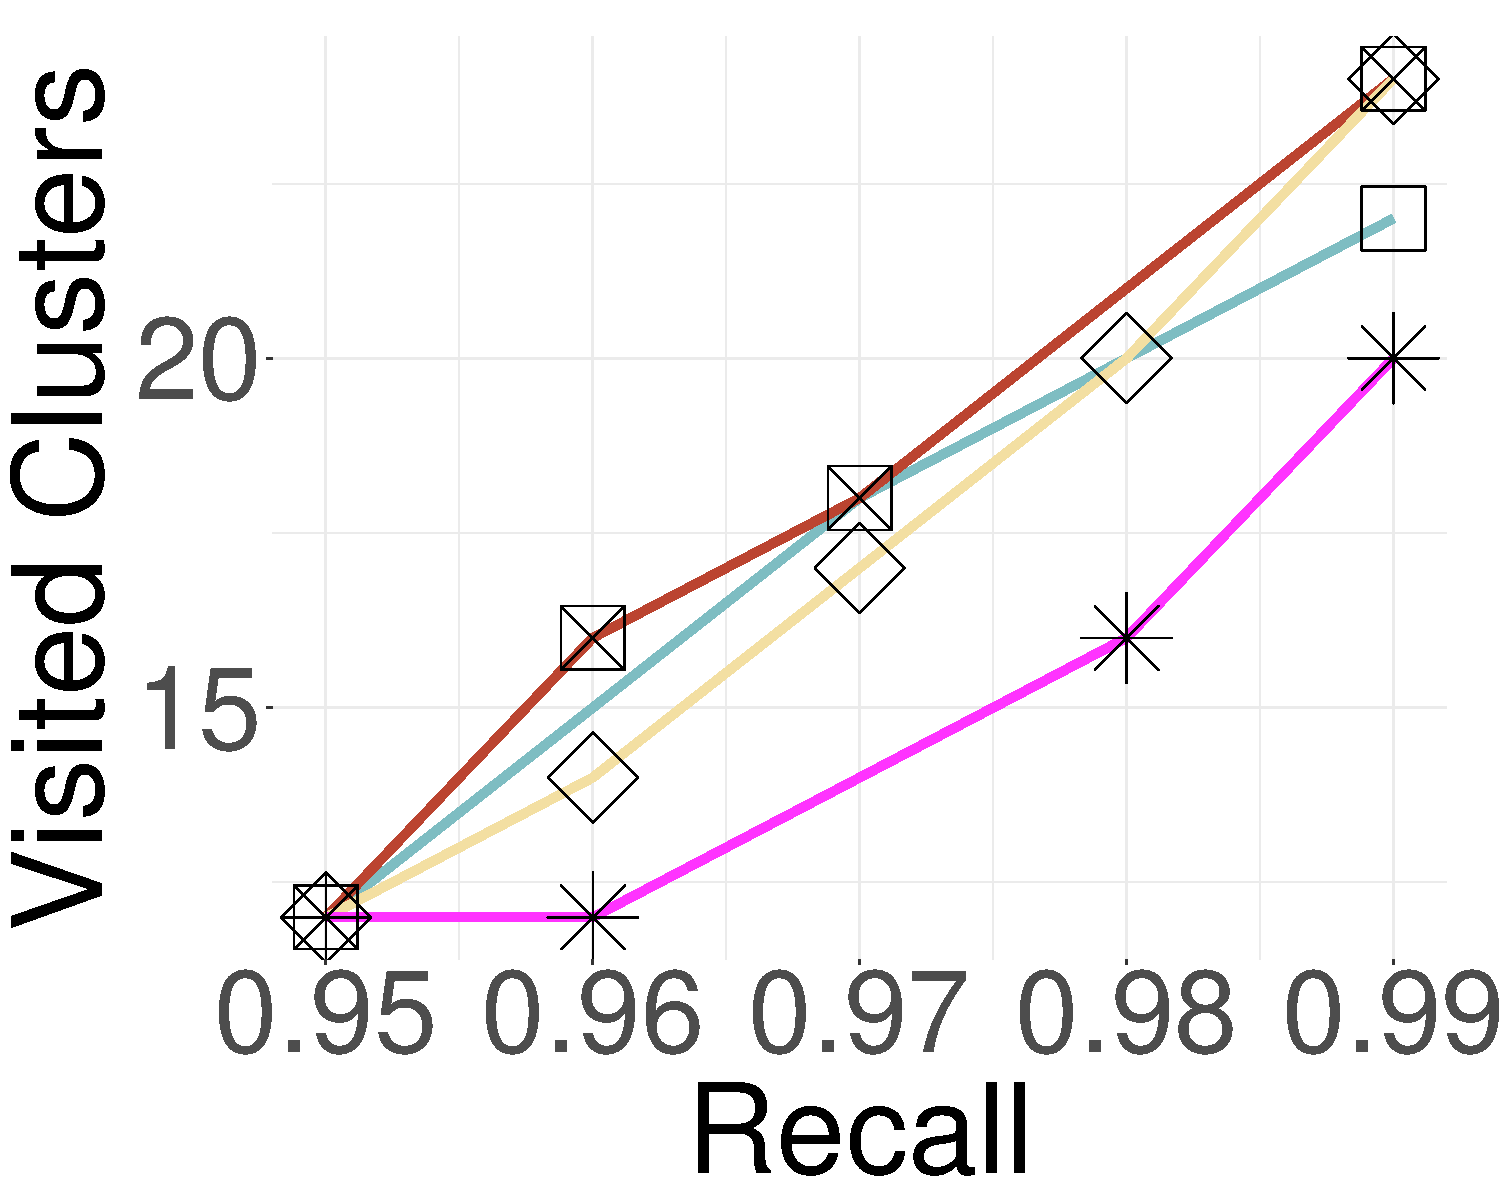
\includegraphics[width=\columnwidth]{../img/elpis/ElpisvsKmeans/qrsnprobes.pdf}                                                             
		\caption{Visited clusters} 
		\label{fig:elpis_kmeans:clusters}
	\end{subfigure}	
	\vspace*{-0.2cm}
	\caption{K-means vs EAPCA (Deep25GB)  } 
	\label{fig:elpis_kmeans}
\end{figure}


We evaluate three different clustering techniques: EAPCA-based clustering, exact K-means and approximate K-means. 
Exact K-means is the K-means algorithm in~\cite{kmeanshistory} that continues iterating until all centroids stabilize. 
Approximate K-means refers to a modified version of the exact K-means which stops execution after a certain number of iterations (user-defined). 
We evaluate different numbers of iterations and choose the one that leads to the same accuracy as the exact K-means. 
For a fair comparison, we use the number of clusters produced by the EAPCA clustering (which is not known in advanced, but determined adaptively) as the number of clusters in both K-means algorithms. 
Note that the points allocated to each cluster may be different across clustering techniques. 
The set of clusters produced by each technique is then fed to the same algorithm, which builds in parallel an HNSW graph in each cluster. 
In the case of ELPIS, the clusters correspond to the EAPCA-based Hercules tree leaves, and the entire tree represents the index. 
For the other techniques, the index consists only of the set of clusters. 
The query answering algorithm within each cluster is the same across techniques, but the pruning of clusters depends on the clustering approach: in the case of EAPCA-based clustering, we search clusters in ascending order of $LB_{EAPCA}$ (lower bounding distance between the query and the EAPCA representations of the clusters), and we prune clusters using both $LB_{EAPCA}$ and $k^{th}_{dist}$, the distance between the query and the current $k^{th}$ bsf answer, obtained by traversing the Hercules tree. 
Both exact and approximate K-means prune clusters based on the distance between the query and the cluster centroids. 
We also evaluate the pruning of the clusters using EAPCA-based clustering with centroid-based pruning (EAPCA-Centroid). EAPCA-Centroid uses the same clusters obtained by the EAPCA clustering, but prunes clusters using the distances to the cluster centroids (instead of $LB_{EAPCA}$ and $k^{th}_{dist}$).


Figure~\ref{fig:elpis_kmeans} summarizes the results of this experiment on the Deep25GB dataset. 
To ensure a fair comparison between EAPCA and K-means, we use the same number of clusters. Since in EAPCA, this number is found adaptively and cannot be enforced, we use the number of leaves that result from building the EAPCA tree as the number of clusters for the K-means algorithms (in the case of Deep25GB, this number is 26). 
The exact K-means algorithm requires 551 iterations to converge, while approximate K-means requires 40 iterations to reach the accuracy levels of exact K-means.
We observe that on average  for a given query, ELPIS delivers the same accuracy as previous methods up to 1.5x faster (Figs.~\ref{fig:elpis_kmeans:proc}-~\ref{fig:elpis_kmeans:distances}). 
At the same time, it builds the index and answers 1 million queries 5x-15x faster than competitors  (Fig.~\ref{fig:elpis_kmeans:idxproc}). 
We report that ELPIS builds its index 4x and 60x faster than the solutions using approximate and exact K-means, respectively, even though they are building the same number of clusters. This is because both exact and approximate K-means spend a significant amount of time to find the centroids and populate them with vectors, whereas ELPIS uses the efficient index building algorithm of Hercules.  
We can see in Figure~\ref{fig:elpis_kmeans:clusters} that the EAPCA clustering, used by ELPIS, achieves the same recall as EAPCA-Centroid by visiting a smaller number of clusters. 
Since they both use the exact same clusters and query algorithm within each cluster, this means that EAPCA prunes the clusters better than EAPCA-Centroid. 
For instance, EAPCA-Centroid needs to visit 20 clusters whereas EAPCA only needs to visit 16. 
Besides, by visiting the same number of clusters, EAPCA can reach a higher recall than EAPCA-Centroid, because it more intelligently selects the most promising clusters to search. 
\subsubsection{Choosing the Graph Structure Within Each Cluster}
In this experiment, we evaluate different state-of-the-art graph structures to choose the best performing one. We divide a dataset into several clusters using the EAPCA dynamic segmentation, then evaluate the indexing and query performance of different types of graphs within the clusters (ELPIS-H using HNSW; ELPIS-N and ELPIS-V using NSG and VAMANA respectively), and compare against the performance of the original graphs. Figure~\ref{fig:elpis:design:graph-type} demonstrates that using HNSW within the clusters leads to the best performance compared to using NSG or VAMANA, in both indexing and query answering.

\begin{figure}[tb]
	\captionsetup{justification=centering}
	\centering	
	\begin{minipage}{\columnwidth}
		\begin{subfigure}{\textwidth}
			\captionsetup{justification=centering}	
			\centering
			
\includegraphics[width=0.8\columnwidth]{../img/elpis/Idx/legend.pdf} 
			\label{fig:idx:time:comParIS+on:Hercules:ParIS+:andromache:coldcache}
		\end{subfigure}\\
		\vspace{-.4in}
	\end{minipage}
			
	\begin{minipage}{0.037\textwidth}
		\captionsetup{justification=centering}
		\captionsetup[subfigure]{justification=centering}
		\begin{subfigure}{\textwidth}		
		
\includegraphics[width=\columnwidth]{../img/Experiments/timeh.pdf}
	\vspace{.5in}	
  \end{subfigure}
	\end{minipage}
	\begin{minipage}{0.27\columnwidth}
	\vspace{0.18in}				
		\begin{subfigure}{\columnwidth}
			\captionsetup{justification=centering}	
			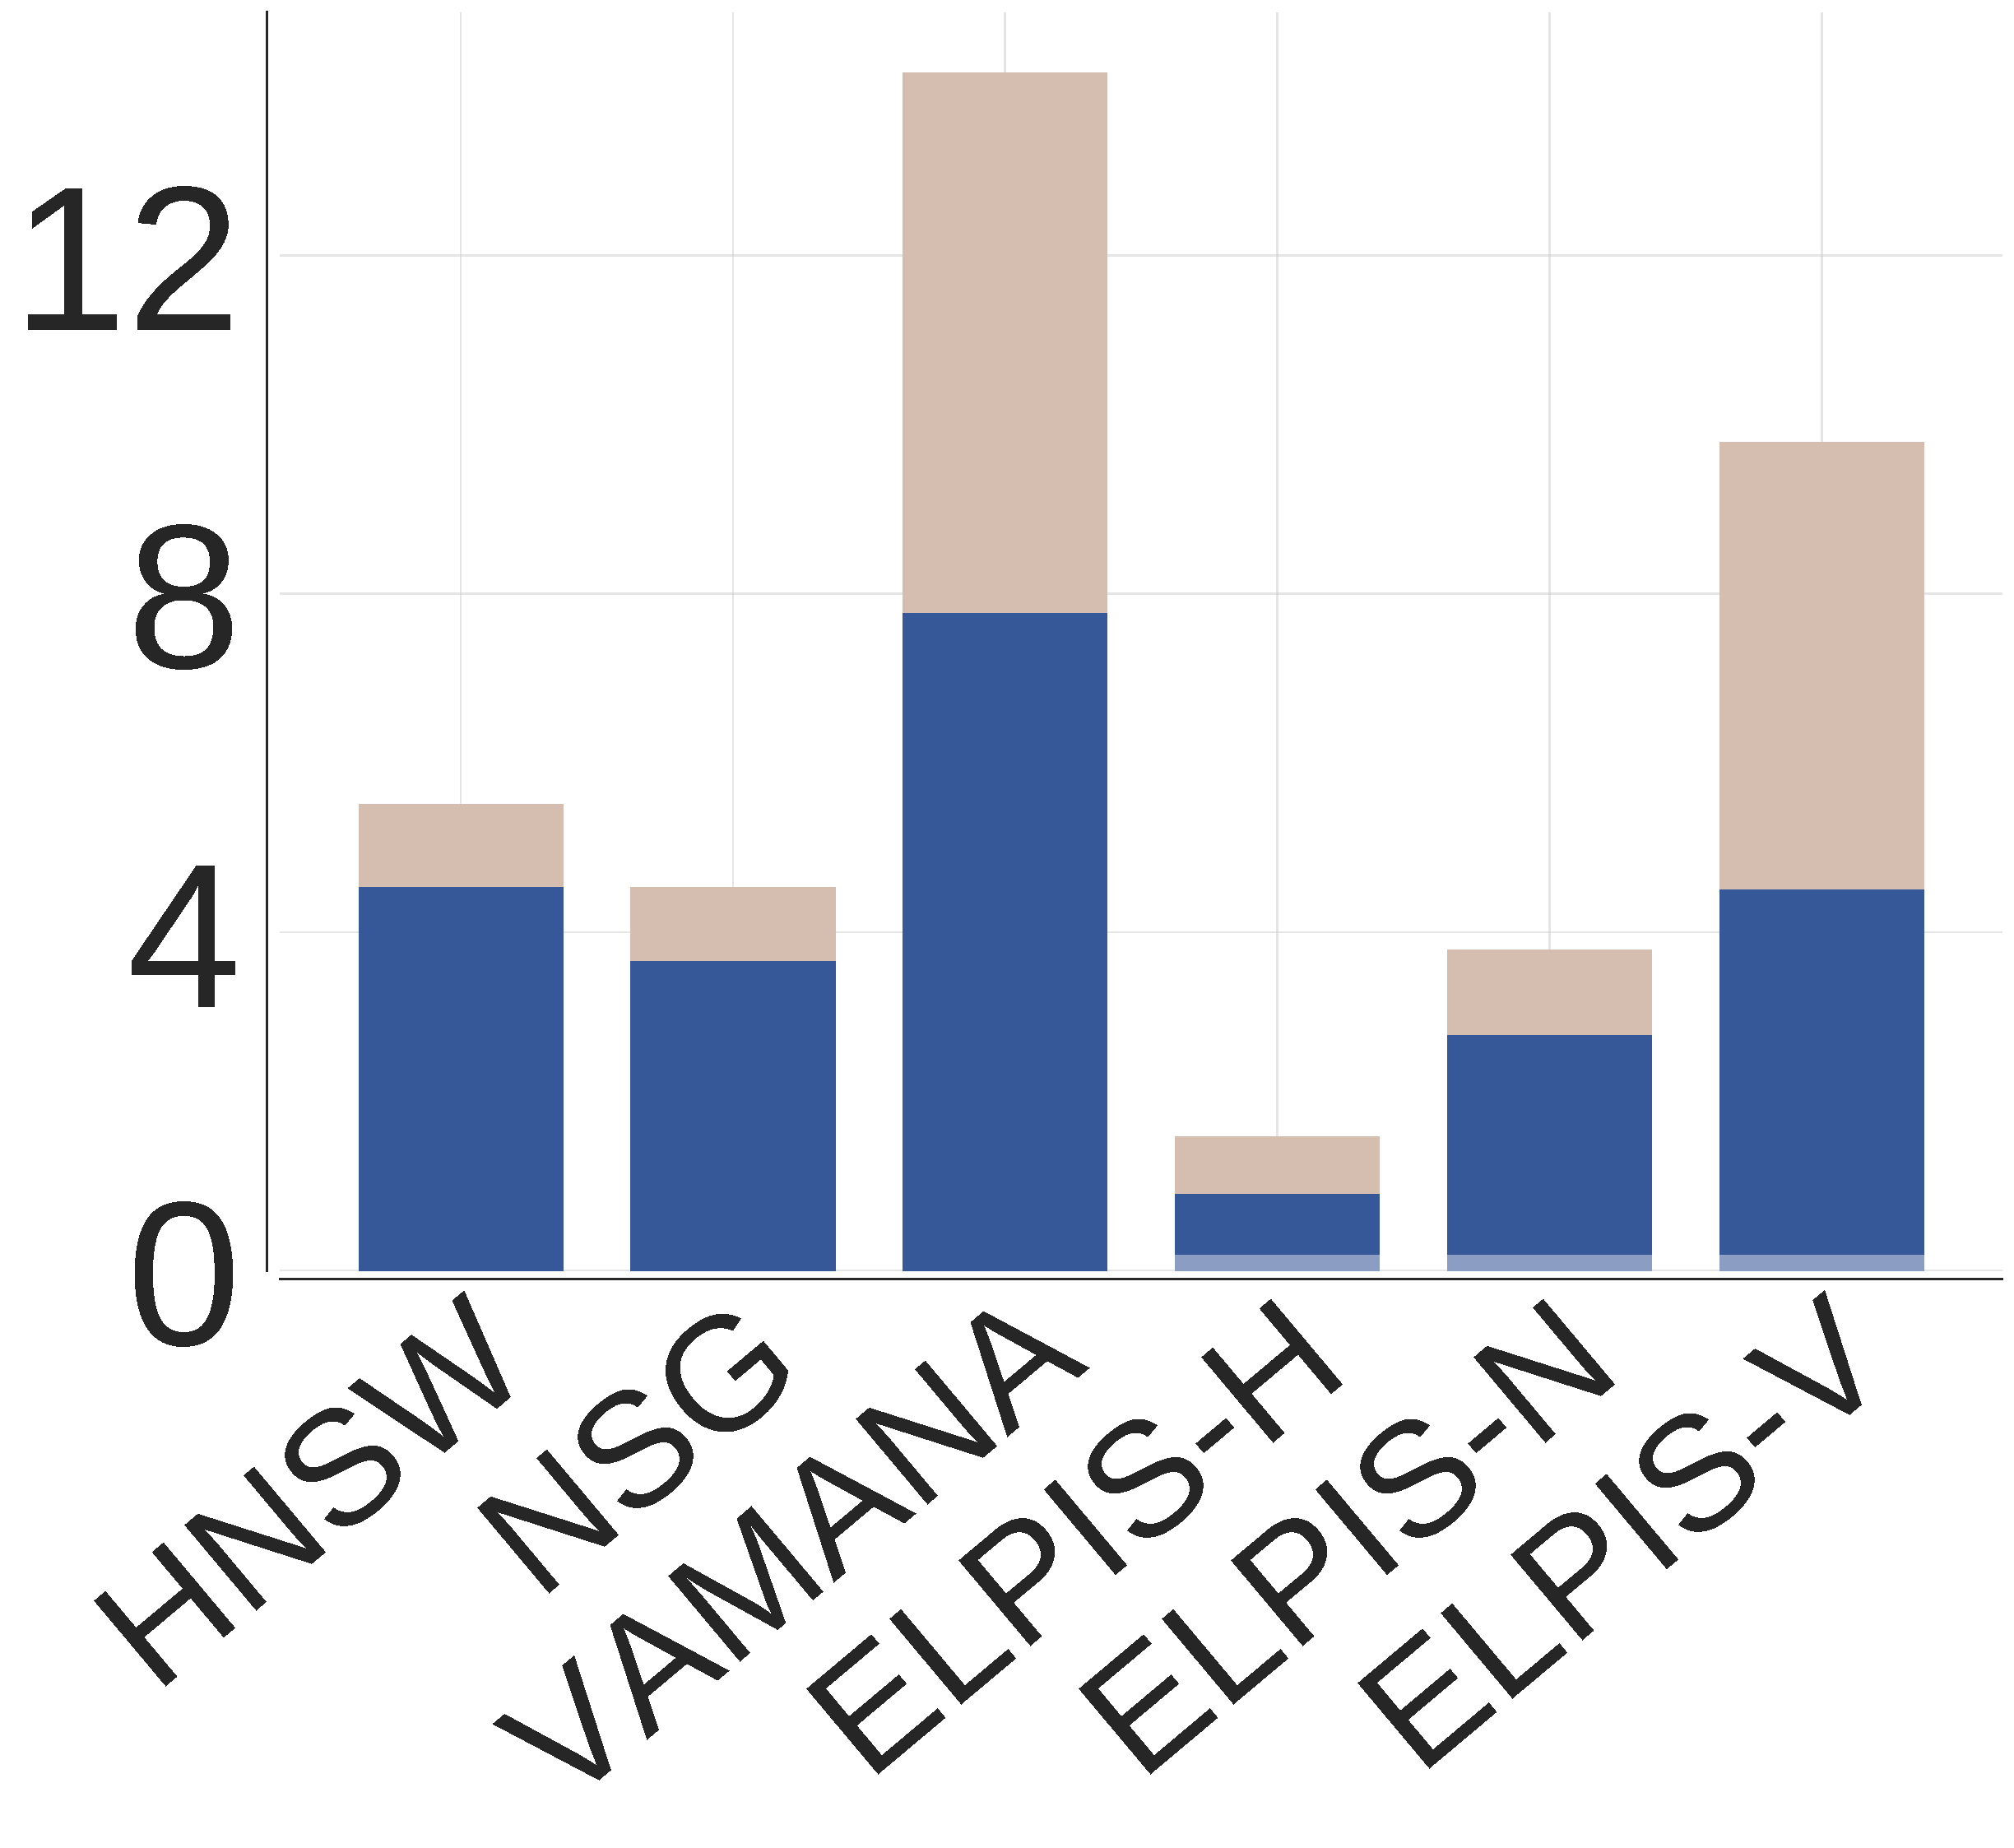
\includegraphics[width=\columnwidth]{../img/elpis/Idx/25_idx_comp.pdf} 
		\end{subfigure}	
	\vspace{-0.27in}
		\caption{{Varying graph structures (Deep25GB)}}
		\label{fig:elpis:design:graph-type}
	\end{minipage}	
	\begin{minipage}{0.295\columnwidth}
		\begin{subfigure}{\columnwidth}
			\includegraphics[width=\columnwidth]{../img/elpis/Idx/25_dpl_comp.pdf} 
		\end{subfigure} 
		\caption{{Varying cluster sizes (Deep25GB)}}
		\label{fig:elpis:design:cluster-size}
	\end{minipage}	
	\begin{minipage}{0.34\columnwidth}				
		\vspace{.05in}
		\begin{subfigure}{\columnwidth}
		\captionsetup{justification=centering}	
			\includegraphics[width=\columnwidth]{../img/elpis/Idx/25_dpl_qps.pdf} 
		\end{subfigure}	
		\caption{{Querying one variable-size cluster (Deep25GB)}}
		\label{fig:elpis:design:cluster-size:errorestqps}
	\end{minipage}
\end{figure}


\subsubsection{Choosing the Number of Clusters}
In this experiment, we show that it is not sufficient to divide the search space to improve the performance of graph-based methods; careful tuning should be applied to find the optimal number of clusters. 
Hercules determines the number of clusters adaptively. It takes as input the maximum amount of data that can fit in one leaf ({\it max\_leaf\_size}), then creates enough leaves to fit similar vectors together in the same leaf. 
Figure~\ref{fig:elpis:design:cluster-size} reports on the x-axis the value of {\it max\_leaf\_size} as a percentage of the size of the dataset, and at the top of each bar, the corresponding number of clusters. 
When the percentage of data is 100, this corresponds to the original HNSW built on the full dataset (i.e., one cluster). 
We observe that splitting the dataset into many small clusters leads to better indexing performance but slower query answering, whereas using a small number of large clusters leads to slower indexing and querying, where the clustering cost becomes marginal compared to the cost of building a graph within each cluster. 
For our experiments, we choose {\it max\_leaf\_size} to be between 5\% and 10\% of the dataset size since it leads to the best trade-off. 
Additionally, we ran an experiment where we vary the size of the clusters and perform the ELPIS search algorithm only on one cluster, keeping all other parameters fixed. 
Figure~\ref{fig:elpis:design:cluster-size:errorestqps} indicates that as the size of a cluster increases, the accuracy improves, but throughput (expressed in Queries Per Second (QPS)) decreases.


\subsection{Index Construction Performance}
We now evaluate the indexing performance of the ten state-of-the-art vector search methods.
We vary the dataset size and report both the indexing total time and footprint. We conduct the experiment using different datasets but, for the sake of space, only report the results for the Deep dataset. The trends are the same across different datasets. The full results can be found in~\cite{url/GASS}.
We use different subsets of the Deep dataset, ranging in size from 1 million to 1 billion vectors, the latter is equivalent to ~350GB. We build the indexes such that each algorithm can achieve a search accuracy of 0.99. 
We first experiment on 1 million vector datasets, reporting results for all methods. However, some methods do not scale to larger sizes and are omitted from the plots. Specifically, on the 25GB datasets, HCNNG, SPTAG-BKT, and SPTAG-KDT exceed 24 hours during index building. Additionally, KGraph and EFANNA require over 300GB and 1.4TB of RAM for 25GB and 100GB datasets, respectively. Consequently, DPG, NSG, and SSG (as they use KGraph and EFANNA) are also omitted from 100GB and larger datasets.



\noindent{\bf Indexing Time.} Figure~\ref{fig:elpis:idx:time} demonstrates that II-based approaches boast the lowest overall indexing time across various dataset sizes. Specifically, the II and DC-based approach, ELPIS, shows significant advantages, being 2.7x faster than HNSW and 4x faster than NSG for both 1M and 25GB dataset sizes. Note that NSG's indexing time includes both the construction of its base graph, EFANNA, which is time-intensive, and the refinement with NSG. SPTAG-BKT and SPTAG-KDT exhibit high indexing times, requiring over 25 hours to index Deep25GB dataset—24 times more than ELPIS, the fastest method. This inefficiency in SPTAG arises from its design, which involves constructing multiple TP Trees and graphs, becoming increasingly costly with larger datasets. On larger datasets 100GB and 1B vectors ($\approx$350GB), only HNSW, ELPIS, and Vamana scale with acceptable indexing time, with ELPIS being 2 and 2.7 times faster than HNSW and Vamana, respectively.


\noindent\textbf{Indexing Footprint.}
Figure~\ref{fig:elpis:idx:footprint:memory} reports the memory footprint for each indexing structure, including the raw data storage. To perform the evaluation, we record the peak virtual memory usage during the index-building phase\footnote{Readings are taken from the proc pseudo filesystem’s Virtual Memory Peak.}. SPTAG-BKT and SPTAG-KDT demonstrate substantial efficiency in memory utilization despite having the highest indexing time. 

They exhibit the lowest indexing memory footprint for 1M and 25GB datasets. For larger datasets, ELPIS has the lowest indexing memory footprint, occupying up to 40\% less memory than HNSW and 30\% less than Vamana during indexing. This is because ELPIS needs a smaller maximum outdegree and beam width compared to its competitors to efficiently build the index. HNSW has a higher indexing memory footprint due to its use of a graph layout optimized for direct access to node edges through a large contiguous block allocation~\cite{url/hnsw}. This layout offers a time advantage over adjacency lists by reducing memory indirections and cache misses. However, it can result in quadratic memory growth when using a large maximum outdegree on large-scale datasets. 
In Figure \ref{fig:elpis:idx:footprint:disk}, we compare the size of method indices, including the raw data. The figure shows that certain methods, such as EFANNA, HCNNG, KGraph, and consequently NSG, SSG, and DPG (which use one of these base graphs), exhibit a significantly larger memory footprint relative to their final index size. For instance, HCNNG consumes substantial memory during indexing, requiring over 200GB for Deep25GB (Fig. \ref{fig:elpis:idx:footprint:memory}) due to merging multiple MST from numerous samples generated during hierarchical clusterings. In contrast, its final index size is less than 50GB (Fig. \ref{fig:elpis:idx:footprint:disk}).

\begin{figure}[!htb]
	\captionsetup{justification=centering}
	\centering	
	\begin{minipage}{\textwidth}
		\begin{subfigure}{\textwidth}
			\centering
			\captionsetup{justification=centering}				\includegraphics[width=\textwidth]{../img/Experiments/legendall.png}
		\end{subfigure}\\
		\vspace{-0.3cm}
	\end{minipage}
	\begin{minipage}{0.28\textwidth}				
	%	\captionsetup{justification=centering}
			\centering
		\begin{subfigure}{\textwidth}
			\captionsetup{justification=centering}	
			\includegraphics[width=\textwidth]{../img/Experiments/Idx_footprint_datasets/idx_time_deep_n.pdf}
		\end{subfigure}	
		\caption{{Indexing Time}}
		\label{fig:elpis:idx:time}
	\end{minipage}	
 \hspace{0.15in}
	\begin{minipage}{0.28\textwidth}				
	%	\captionsetup{justification=centering}
		\begin{subfigure}{\textwidth}
			\centering
			\captionsetup{justification=centering}	
			\includegraphics[width=\textwidth]{../img/Experiments/Idx_footprint_datasets/idx_footprint_deep_n.pdf}
		\end{subfigure}	
		\caption{{Indexing Memory Footprint}}
		\label{fig:elpis:idx:footprint:memory}
	\end{minipage}	
 \hspace{0.15in}
	\begin{minipage}{0.29\textwidth}				
	%	\captionsetup{justification=centering}
		\begin{subfigure}{\textwidth}
			\centering
			\captionsetup{justification=centering}	
			\includegraphics[width=\textwidth]{../img/Experiments/Idx_footprint_datasets/idx_indexsize_deep_n.pdf}
		\end{subfigure}	
		\caption{{Indexing Disk Footprint}}
		\label{fig:elpis:idx:footprint:disk}
	\end{minipage}		
	\begin{minipage}{0.28\textwidth}				
		%	\captionsetup{justification=centering}
		\begin{subfigure}{\textwidth}
			\centering
			\captionsetup{justification=centering}	
			\includegraphics[width=\textwidth]{../img/Experiments/Idx_footprint_datasets/search_footprint_deep_n.pdf}
		\end{subfigure}	
		\caption{{Query Memory Footprint}}
		\label{fig:elpis:query:footprint:memory}
	\end{minipage}	
 \hspace{0.15in}
	\begin{minipage}{0.28\textwidth}
		\centering
		\begin{subfigure}{\textwidth}
			\includegraphics[width=\textwidth]{../img/Experiments/Idx_footprint_datasets/qrs_beamwidth_n.pdf}
		\end{subfigure} 
		\caption{{Query Beam Width}}
		\label{fig:elpis:query:beam-width}
	\end{minipage}
\end{figure}

\subsection{Search Performance}
We now evaluate the query-answering performance of the different methods. Some methods are omitted because the indexes could not be built on large datasets (NSG, SSG, SPTAG-BKT, DPG, EFANNA, SPTAG-KDT, HCNNG, KGraph). Other methods were not included in some 25GB plots (KGraph, DPG, SPTAG-KDT, HCNNG, and EFANNA) for the sake of clarity since their query-answering times were significantly higher than the best baselines. The full results can be found in~\cite{url/GASS}.  

\noindent\textbf{Query Memory Footprint and Beam Width.} 
Figure~\ref{fig:elpis:query:footprint:memory} for the Deep dataset indicates that Vamana, followed by ELPIS, have the lowest memory footprint during search. Even though ELPIS has a smaller index size, it adopts a contiguous memory storing during search, which increases the index footprint when loaded into memory. Besides, Figure~\ref{fig:elpis:query:beam-width} shows that ELPIS requires the smallest beam width to reach similar query accuracy. A very high beam width indicates that the beam search needs to visit a wider area and make more distance calculations to retrieve the nearest neighbor (NN) answers.

\noindent\textbf{Real Datasets.}  On the datasets with 1M vectors (Figure~\ref{fig:elpis:query:performance:1M}), ELPIS and NSG are the best performers on Sift1M and Seismic1M. NSG maintains its leading position in Deep1M, while HCNNG shows the best performance for SALD1M. 

When moving to 25GB datasets (Figure~\ref{fig:elpis:query:performance:25GB}), SSG and HCNNG experience a drop in performance, and ELPIS takes the lead with the best overall performance, except for SALD25GB, where SPTAG-BKT wins on high accuracy. It is worth noting that none of the methods achieved an accuracy over 0.8 on the Seismic dataset, leading us to report results for these lower recall values. The significant indexing footprint of NSG prevented us from extending its evaluation to larger datasets, as constructing the EFANNA graph (which NSG depends on) requires more memory than the available 1.4TB. 

For hard query workloads in Figure~\ref{fig:search:query:performance:25GB:hard}, we compare the best-performing methods from the two most performing graph paradigms, ND-based and DC-based methods, including HNSW, NSG, ELPIS, and SPTAG-BKT. SPTAG-BKT achieves the overall best performance for the 1\% noise query set. As we increase the noise up to 10\%, SPTAG-BKT's performance deteriorates, which we can attribute to the SPTAG-BKT structure failing to identify good seed points. At the same time, the other competitors gain an advantage, with ELPIS taking the lead. 

When analyzing very large datasets of 1 billion vectors, Figure~\ref{fig:elpis:query:performance:1B} shows the superiority of ELPIS, which is up to an order of magnitude faster at achieving 0.95 accuracy, thanks to its design that supports multi-threading for query answering. This trend is consistent across subsets ranging from 100GB (Figure~\ref{fig:elpis:query:performance:100GB}) to 250GB (detailed results are reported in~\cite{url/GASS}).

\noindent{\bf Data Distributions.} We assess top performers from different classes of paradigms (EFANNA, Vamana, SSG, HNSW, ELPIS, and SPTAG-BKT) on challenging datasets (Fig.~\ref{fig:datacomp}) and report the results in Figures~\ref{fig:query:performance:25GB:rand:pow1:10NN} and~\ref{fig:query:performance:25GB:rand:pow50:10NN}. We observe that ELPIS consistently achieves high accuracy across skewness levels (0 to 50), outperforming other methods. As dataset skewness increases and search becomes easier, most graph-based approaches improve, but ELPIS still maintains its superiority.


\newcommand{\soneM}{0.28}
\newcommand{\spbf}{0.13in}
\begin{figure}[!htb]
	\captionsetup{justification=centering}
	\centering
		\begin{subfigure}{\textwidth}
			\includegraphics[width=\textwidth]{../img/Experiments/legendall.png}
		\end{subfigure}	
  
	\captionsetup[subfigure]{justification=centering}
	\begin{subfigure}{\soneM\textwidth}
		\centering
		\includegraphics[width=\textwidth]{../img/Experiments/search/1M/sift_10nn.pdf}
		\caption{\textbf{Sift1M}} 
	
 \label{fig:elpis:query:performance:1M:sift:10NN}
	\end{subfigure}
   \hspace{0.4cm}
	\begin{subfigure}{\soneM\textwidth}
		\centering
		\includegraphics[width=\textwidth]{../img/Experiments/search/1M/deep_10nn.pdf}
		\caption{\textbf{Deep1M}} 
		\label{fig:elpis:query:performance:1M:deep:10NN}
	\end{subfigure}
   \hspace{0.4cm}
	\begin{subfigure}{\soneM\textwidth}
		\centering
		\includegraphics[width=\textwidth]{../img/Experiments/search/1M/sald_10nn.pdf}
		\caption{\textbf{SALD1M}} 
		\label{fig:elpis:query:performance:1M:sald:10NN}
	\end{subfigure}
 
	\begin{subfigure}{\soneM\textwidth}
		\centering
		\includegraphics[width=\textwidth]{../img/Experiments/search/1M/seismic_10nn.pdf}
		\caption{\textbf{Seismic1M}} 
		\label{fig:elpis:query:performance:1M:seismic:10NN}
	\end{subfigure}
   \hspace{0.4cm}
	\begin{subfigure}{\soneM\textwidth}
		\centering
		\includegraphics[width=\textwidth]{../img/Experiments/search/1M/gist_10nn.pdf}
		\caption{\textbf{Gist1M}} 
		\label{fig:elpis:query:performance:1M:gist:10NN}
	\end{subfigure}
   \hspace{0.4cm}
 	\begin{subfigure}{\soneM\textwidth}
		\centering
		\includegraphics[width=\textwidth]{../img/Experiments/search/1M/imagenet_10nn.pdf}
		\caption{\textbf{ImageNet1M}} 
		\label{fig:elpis:query:performance:1M:imagenet:10NN}
	\end{subfigure}
	\vspace*{-0.2cm}
	%\caption{{\color{black} Efficiency vs. accuracy in memory (100 queries)}}	surat al mulk
	%	\caption{{Efficiency vs. accuracy (Dataset = 1M, Queries = 100, k = 10) }}	
	\caption{Query performance on 1M vectors}	
	\vspace*{-0.2cm}
	\label{fig:elpis:query:performance:1M}
\end{figure}


    \newcommand{\soneMs}{0.155}
\renewcommand{\soneM}{0.25}
\renewcommand{\spbf}{0.0in}
\begin{figure}[!htb]
	\captionsetup{justification=centering}
	\centering
		\begin{subfigure}{\textwidth}
			\includegraphics[width=\textwidth]{../img/Experiments/legendall.png}
		\end{subfigure}	
 
	\begin{minipage}{\textwidth}
 \centering
		\captionsetup{justification=centering}
		\captionsetup[subfigure]{justification=centering}
	 \begin{comment}
 \begin{minipage}{0.05\textwidth}
		\captionsetup{justification=centering}
		\captionsetup[subfigure]{justification=centering}
		\begin{subfigure}{\textwidth}
		\vspace*{-.7in}
		\includegraphics[width=0.6\columnwidth]{../img/Experiments/time.pdf}
		\vspace*{.6in}
		\includegraphics[width=0.6\columnwidth]{../img/Experiments/time.pdf}
		\end{subfigure}
	\end{minipage}
  \end{comment}

		\begin{subfigure}{\soneM\textwidth}
  \centering
			\includegraphics[width=\textwidth]{../img/Experiments/search/25/deep_10nn.pdf}
			\caption{Deep}  
		\label{fig:elpis:query:performance:25GB:deep:10NN}
		\end{subfigure}
   \hspace{0.4cm}
		\begin{subfigure}{\soneM\textwidth}
  \centering
			\includegraphics[width=\textwidth]{../img/Experiments/search/25/sald_10nn.pdf}
			\caption{SALD}  
		\label{fig:elpis:query:performance:25GB:sald:10NN}
		\end{subfigure}
  \hspace{0.4cm}
		\begin{subfigure}{\soneM\textwidth}
  \centering
			\includegraphics[width=\textwidth]{../img/Experiments/search/25/seismic_10nn.pdf}
			\caption{Seismic}  
			\label{fig:elpis:query:performance:25GB:seismic:10NN}
		\end{subfigure}	
  
		\begin{subfigure}{\soneM\textwidth}
  \centering
			\includegraphics[width=\textwidth]{../img/Experiments/search/25/sift_10nn.pdf}
			\caption{Sift}  
			\label{fig:elpis:query:performance:25GB:sift:10NN}
		\end{subfigure}
   \hspace{0.4cm}
	\begin{subfigure}{\soneM\textwidth}
 \centering
		\includegraphics[width=\textwidth]{../img/Experiments/search/25/pow1_10nn.pdf}
		\caption{\textbf{RandPow0}} 
		\label{fig:query:performance:25GB:rand:pow1:10NN}
	\end{subfigure}
   \hspace{0.4cm}
	\begin{subfigure}{\soneM\textwidth}
 \centering
		\includegraphics[width=\textwidth]{../img/Experiments/search/25/pow50_10nn.pdf}
		\caption{\textbf{RandPow50}} 
		\label{fig:query:performance:25GB:rand:pow50:10NN}
	\end{subfigure}		
		\caption{{25GB datasets}}
		\label{fig:elpis:query:performance:25GB}
	\end{minipage}
\end{figure}

\renewcommand{\soneM}{0.28}
\begin{figure}[!htb]
\captionsetup{justification=centering}
	\centering
		\begin{subfigure}{\textwidth}
			\includegraphics[width=\textwidth]{../img/Experiments/legendall.png}
		\end{subfigure}	
		\captionsetup{justification=centering}
		\captionsetup[subfigure]{justification=centering}
		\begin{subfigure}{\soneM\textwidth}
  \centering
		\includegraphics[width=\textwidth]{../img/Experiments/search/25/deep1p_10nn.pdf}
		\caption{\textbf{1\% noise}} 
		\label{fig:search:query:performance:25GB:hard:1p}
		\end{subfigure}
    \hspace{0.4cm}
  		\begin{subfigure}{\soneM\textwidth}
  \centering
		\includegraphics[width=\textwidth]{../img/Experiments/search/25/deep5p_10nn.pdf}
		\caption{\textbf{5\% noise}} 
		\label{fig:search:query:performance:25GB:hard:1p}
		\end{subfigure}
    \hspace{0.4cm}
		\begin{subfigure}{\soneM\textwidth}
  \centering
		\includegraphics[width=\textwidth]{../img/Experiments/search/25/deep10p_10nn.pdf}
		\caption{\textbf{10\% noise}} 
		\label{fig:search:query:performance:25GB:hard:10p}
		\end{subfigure}
	\caption{Search Performance on Varying workloads difficulty}
		\label{fig:search:query:performance:25GB:hard}
	\end{figure}

 \begin{figure}[!htb]
		\captionsetup{justification=centering}
		\captionsetup[subfigure]{justification=centering}
  	\centering
		\begin{subfigure}{\textwidth}
			\includegraphics[width=\textwidth]{../img/Experiments/legendall.png}
		\end{subfigure}	
		\begin{subfigure}{\soneM\textwidth}
  \centering
			\includegraphics[width=\textwidth]{../img/Experiments/search/100/deep_10nn.pdf}
			\caption{Deep}  
		\label{fig:elpis:query:performance:100GB:deep:10NN}
		\end{subfigure}
    \hspace{0.4cm}
		\begin{subfigure}{\soneM\textwidth}
  \centering
			\includegraphics[width=\textwidth]{../img/Experiments/search/100/sift_10nn.pdf}
			\caption{Sift}  
		\label{fig:elpis:query:performance:100GB:sift:10NN}
		\end{subfigure}
    \hspace{0.4cm}
  		\begin{subfigure}{\soneM\textwidth}
  \centering
			\includegraphics[width=\textwidth]{../img/Experiments/search/100/sald_10nn.pdf}
			\caption{Sald}  
		\label{fig:elpis:query:performance:100GB:sald:10NN}
		\end{subfigure}
		\caption{{Search Performance on 100GB datasets}}	
		\label{fig:elpis:query:performance:100GB}
	\end{figure}
 
	\begin{figure}
		\captionsetup{justification=centering}
		\captionsetup[subfigure]{justification=centering}
  	\centering
		\begin{subfigure}{\textwidth}
			\includegraphics[width=\textwidth]{../img/Experiments/legendall.png}
		\end{subfigure}	
		\begin{subfigure}{\soneM\textwidth}
			\includegraphics[width=\textwidth]{../img/Experiments/search/1B/deep_10nn.pdf}
			\caption{Deep}  
		\label{fig:elpis:query:performance:1B:deep:10NN}
		\end{subfigure}
    \hspace{0.4cm}
		\begin{subfigure}{\soneM\textwidth}
			\includegraphics[width=\textwidth]{../img/Experiments/search/1B/sift_10nn.pdf}
			\caption{Sift}  
			\label{fig:elpis:query:performance:1B:sift:10NN}
		\end{subfigure}
    \hspace{0.4cm}
  		\begin{subfigure}{\soneM\textwidth}
			\includegraphics[width=\textwidth]{../img/Experiments/search/1B/text2img_10nn.pdf}
			\caption{Text-to-Image}  
			\label{fig:elpis:query:performance:1B:t2i:10NN}
		\end{subfigure}
		\caption{{Search Performance on 1B datasets}}	
		\label{fig:elpis:query:performance:1B}
	\end{figure}

\section{Discussion}
\label{sec:discussion}
In the previous section, we reported the results of our extensive experimental evaluation
of ten state-of-the-art graph-based vector search methods, including ELPIS.
Table~\ref{tab:comp} summarizes the evaluation across key criteria: % for both search and indexing. 
for search, we assess efficiency, accuracy, and the number of tunable parameters; 
for indexing, we evaluate efficiency at high recall, memory footprint, and parameter tuning complexity. 

The best-performing methods, HNSW, VAMANA, and ELPIS, have the best search performance and index efficiency. However, ELPIS requires an extra parameter during both indexing (leaf size) and search (nprobes), whereas VAMANA requires an extra parameter to tune during indexing (alpha). NSG and SSG exhibit efficient query performance, but their indexing capability is hindered because of their base graph EFANNA, which similarly to KGraph, is tedious to tune and suffers from high indexing time and footprint. Both SPTAG (BKT) and NGT show satisfactory performance during search; however, they do not scale well to large datasets and require more tuning compared to the best methods. The assessment of HCCNG is based on the optimized parlayNN implementation which has shown competitive performance on large-scale datasets~\cite{parlayann}.

\begin{table}[ht]
\begin{minipage}{0.8\textwidth}
\hspace{3.5cm}
$\checkmark$ Good \quad
$\sim$ Medium \quad
$\times$ Bad
\end{minipage} \\[2pt]
\captionsetup{justification=centering}
\resizebox{\columnwidth}{!}{
\begin{tabular}{lccc|ccc}
\toprule
\textbf{Method} & \multicolumn{3}{c|}{\textbf{Query Answering}} & \multicolumn{3}{c}{\textbf{Index Building}} \\
                & \textbf{Efficiency} & \textbf{Accuracy} & \textbf{Tuning} & \textbf{Efficiency} & \textbf{Footprint} & \textbf{Tuning} \\
\midrule
HNSW     & $\checkmark$ & $\checkmark$ & $\checkmark$ & $\checkmark$ & $\checkmark$ & $\checkmark$ \\
ELPIS    & $\checkmark$ & $\checkmark$ & $\sim$       & $\checkmark$ & $\checkmark$ & $\sim$ \\
VAMANA   & $\checkmark$ & $\checkmark$ & $\checkmark$ & $\checkmark$ & $\checkmark$ & $\sim$ \\
NSG      & $\checkmark$ & $\checkmark$ & $\checkmark$ & $\sim$       & $\sim$       & $\sim$ \\
SSG      & $\checkmark$ & $\checkmark$ & $\checkmark$ & $\sim$       & $\sim$       & $\sim$ \\
EFANNA   & $\times$     & $\sim$       & $\times$     & $\times$     & $\times$     & $\times$ \\
KGRAPH   & $\times$     & $\times$     & $\times$     & $\times$     & $\times$     & $\times$ \\
DPG      & $\times$     & $\sim$       & $\sim$       & $\sim$       & $\sim$       & $\sim$ \\
SPTAG    & $\checkmark$       & $\checkmark$ & $\times$     & $\times$     & $\checkmark$ & $\times$ \\
HCNNG    & $\checkmark$ & $\checkmark$ & $\checkmark$ & $\checkmark$ & $\checkmark$ & $\sim$ \\
LSHAPG   & $\times$     & $\sim$       & $\times$     & $\sim$       & $\checkmark$ & $\checkmark$ \\
NGT      & $\checkmark$       & $\checkmark$       & $\times$     & $\sim$       & $\checkmark$ & $\times$ \\
\bottomrule
\end{tabular}

}
\centering
\caption{Comparative analysis}
	%\vspace*{-0.4cm}
\label{tab:comp}
\end{table}


We now summarize the key insights from both experiments, focusing on state-of-the-art approaches and different key components of graph methods, i.e., Seed Selection and Neighborhood Diversification.

\noindent{\bf Unexpected Results.} Our results reveal some interesting observations that warrant further investigation. 
\textit{(1) Stacked NSW:} while hierarchical layers of NSW graphs have shown promise in improving search performance on billion-scale datasets (Figure~\ref{fig:ss:search}), our experiments demonstrate that a simpler approach like K-random sampling can achieve better results on smaller and medium-sized datasets. 

\textit{(2) Scalability of Graph Approaches:} While all graph-based vector search methods can efficiently build indexes on small datasets, most approaches face significant scalability challenges. Some methods (SPTAG-BKT, NSG, and SSG) demonstrate impressive search performance on 1M and 25GB datasets (Figs.~\ref{fig:elpis:query:performance:1M:sift:10NN},~\ref{fig:elpis:query:performance:1M:deep:10NN},~\ref{fig:elpis:query:performance:25GB:seismic:10NN},~\ref{fig:elpis:query:performance:25GB:deep:10NN}, and~\ref{fig:elpis:query:performance:25GB:sald:10NN}) but their index construction could not scale to 100GB and billion-scale datasets. An important research direction is to improve the indexing scalability for these methods, either by adopting summarization techniques during index construction or by using a scalable data structure to construct the base graph (i.e., IVFPQ~\cite{faiss} to find the neighbors of nodes during insertion).

\textit{(3) DC-based approach for hard datasets and workloads:} An interesting finding was the superior performance of DC-based approaches, specifically ELPIS and SPTAG-BKT, compared to other methods like HNSW, NSG, SSG, and Vamana on challenging datasets and workloads such as Seismic, RandPow0, RandPow50, and Deep hard query workloads for 1M and 25GB dataset sizes. We believe the DC strategy helps in this context because the graphs are built on clustered subsets of data, which facilitates beam search in retrieving more accurate nearest neighbors (NN), as opposed to running the search on the entire dataset, which results in lower accuracy (Figures~\ref{fig:elpis:query:performance:1M:seismic:10NN},~\ref{fig:elpis:query:performance:25GB:seismic:10NN},~\ref{fig:query:performance:25GB:rand:pow1:10NN}, and~\ref{fig:query:performance:25GB:rand:pow50:10NN}).

\noindent{\bf Neighborhood Diversification.} Adopting an ND strategy to sparsify the graph \textit{always} leads to better search performance, particularly as the dataset size grows (Figures~\ref{fig:elpis:query:performance:1M:seismic:10NN},~\ref{fig:elpis:query:performance:25GB:seismic:10NN}). Our experiments also show that RND and MOND lead to the best search performance overall (Figure~\ref{fig:ND:search:real}). Nevertheless, we believe there is significant room for improvement in this direction. Additionally, further theoretical studies are necessary to better understand the trade-offs between proximity and sparsity, in order to build graph structures that are efficient during search while maintaining good connectivity.

\noindent{\bf Seed Selection.} Our experiments demonstrate that the SS strategy plays a crucial role in enhancing not only search performance (Figure~\ref{fig:ss:search}) but also indexing efficiency (Table~\ref{tab:ss:idx}). An important research direction is to develop novel, lightweight SS strategies. Such strategies could significantly improve the overall performance of graph-based vector search, both in terms of indexing and query-answering. Additionally, they could enhance the ability to handle out-of-distribution queries, particularly for large datasets where efficient seed selection becomes even more critical (Figures~\ref{fig:ss:deep1b},~\ref{fig:ss:sift1b}).

\noindent{\bf Data-Adaptive Techniques.} Our experiments evaluate the performance of various graph-building paradigms within our proposed taxonomy (SS, NP, II, ND, and DC). While NP-based methods perform the worst overall and are the least scalable, there is no clear winner across all dataset sizes and query workloads. \textit{(1) Scalability:} II-based approaches demonstrate superior efficiency during indexing and achieve higher scalability in both querying and indexing. \textit{(2) Query Answering:} ND-based methods have the best query performance overall. Meanwhile, DC-based approaches are superior on challenging datasets (High LID \& Low RC, Fig.~\ref{fig:datacomp}) and hard query workloads. A promising research direction would be to develop techniques that adapt to dataset characteristics such as dataset size, dimensionality, RC, and LID to excel both in indexing and query answering across a variety of query workloads and dataset sizes.

\noindent{\bf Hybrid Design.} Most recent methods use a mix of paradigms. HNSW leverages II to scale index construction to large datasets and ND to support efficient query answering. ELPIS incorporates a DC-based strategy during both index building and search to further enhance the scalability of HNSW across varying dataset difficulty levels. Interestingly, Vamana, relying only on the ND paradigm, achieves impressive search performance and scalability; however, its indexing time is prohibitive. A promising research direction is building hybrid approaches that combine the key strengths of different techniques, particularly II, ND, and DC. Additionally, devising novel base graphs, clustering, and summarization techniques tailored for DC-based methods can further improve their performance.

\noindent{\bf Recommendations.}
Our study demonstrates varying performance trends across datasets of different sizes, query workloads of different hardness and desired recall values. Figure~\ref{fig:recgann} provides recommendations for methods based on these criteria.  For small to medium-sized datasets (25GB and below), HNSW, NSG, and its improved version, SSG, consistently demonstrate excellent performance on easier datasets (Fig.\ref{fig:elpis:query:performance:1M:deep:10NN}, \ref{fig:elpis:query:performance:1M:sift:10NN}, \ref{fig:elpis:query:performance:1M:imagenet:10NN}, \ref{fig:elpis:query:performance:1M:gist:10NN}).  On harder datasets, DC-based methods like SPTAG, ELPIS, and HCNNG prove more efficient (Figs. \ref{fig:elpis:query:performance:1M:seismic:10NN} \ref{fig:elpis:query:performance:25GB:seismic:10NN}, \ref{fig:elpis:query:performance:1M:sald:10NN}, \ref{fig:elpis:query:performance:25GB:sald:10NN}, \ref{fig:search:query:performance:25GB:hard:1p}, \ref{fig:search:query:performance:25GB:hard:10p}). 
On large datasets (100GB and above), HNSW and ELPIS consistently rank as top choices (Figs.\ref{fig:elpis:query:performance:100GB}, \ref{fig:elpis:query:performance:1B}). 

\begin{figure}
\centering
  \captionsetup{justification=centering}
    \includegraphics[width=0.6\columnwidth]{img/Experiments/recgann.png}
	 \caption{Recommendations (Indexing + 10K queries} 
    \label{fig:recgann}
	
\end{figure}

\section{Conclusion}
In this chapter, we presented ELPIS, our new approach for vector search that exploits both Graph and tree structure to leverage the power of both families of structures for efficient indexing and search performance. We have compared empirically ELPIS with twelve state-of-the-art methods for graph-based vector search, and discussed how the performance of many approaches can degrade on large size data where few succeed to scale. We also discussed the basic incremental insertion graph performance under different key components for seed selection and neighborhood diversification.
In the next section, we will present a new method for graph-based similarity search, that improves the efficiency of the search and indexing, based on the insights we have from our experimental study.

\graphicspath{{../img/experiments/}}
\chapter{ELPIS+: Throughput-Optimized
Graph-Based Vector Search}
\chaptermark{ELPIS+: Throughput-Optimized Graph Vector Search}
\label{chapter:elpis2}
In the previous chapter, we presented ELPIS, a novel graph-based approach for vector similarity search designed for latency-optimized workloads.
%Vector Approximate search is a core operation in various domains and machine learning applications. Various families of methods have been proposed, among them, graph-based methods are undeniably the best for ng-approximate search. 
In this chapter, we introduce ELPIS+, an extension of ELPIS that is optimized for both latency and throughput. We show that ELPIS requires small leaves to reduce query latency, but larger leaves to increase query throughput. Since indexing scalability is an important bottleneck for graph-based vector search methods, the naive solution of building a separate index for each scenario is impractical. Therefore, we propose a novel graph merging strategy that exploits the same ELPIS indexing structure (i.e, graph indexes are built once) to efficiently support both scenarios. Note that parallelizing beam search on the same graph-based index is challenging due to the sequential dependencies of node expansions and the need for synchronized access to shared data structures, leading to contention and inefficiencies in parallel execution, making it an open research problem~\cite{leiserson2010work, speedann}.
%limits of ELPIS approach. We eventually present the variation of ELPIS for throughput, that demand a large leaf size. We eventually then propose a new approach to merge the ELPIS graph leaves, EAPCA-based Merging, into larger size instead of building the graphs of large leaves from scratch. This approach will enable us to adapt Elpis to throughput efficienty  by merging its leaves without building the new graphs from scratch.
\clearpage

\section{ELPIS For Throughput}
ELPIS is a state-of-the-art method for graph-based vector search that combines both graphs and trees. ELPIS exploits multi-threading during search by splitting its search space based on the EAPCA tree. During search, ELPIS prunes the search space in two steps, first ELPIS prunes the unpromising leaves with the EAPCA lower-bounding distance, then uses the graph indices to prune the remaining candidates. This paradigm allows ELPIS to support efficient indexing and search. However, ELPIS requires small leaves to achieve low query latency and large leaves to reach high throughput.  
%, ELPIS requires small leaves, while improving throughout leavesthe search of ELPIS mainly focuses on latency, which reflects the search time to answer one query. Nevertheless, as we move to multiple query parallel search, ELPIS face major challenges, as it requires more number threads to run across the different queries in parallel, as it already exploits multiple threads to answer each query.


\begin{figure}[tb] 
\centering
		\captionsetup{justification=centering}
  		\includegraphics[width=0.4\columnwidth]{../img/elpis2/pre/legendpre.png}
    
		\includegraphics[width=0.4\columnwidth]{../img/elpis2/pre/deep_Time.png}
		\caption{Parallel batch query workload (Deep100GB)}       
		\label{fig:elpis2:pre}
 \end{figure}

Figure~\ref{fig:elpis2:pre}
 compares the performance of ELPIS on a batch query workload, where multiple queries are run in parallel (ELPISPMQS), to HNSW on the same setting (HNSWPMQS). We straightforwardly adapt both methods by assigning different queries to different threads. We remark that the performance of ELPIS on multiple queries lag behind that of HNSW. This is mainly due the fact that ELPIS assigns multiple threads to each query, while HNSW dedicates one thread to each query, thereby achieving a higher throughput.
 
To address this issue, we introduce two main changes to ELPIS for batch query workload scenario: i) we minimize the number of threads required to answer one query by increasing the maximum size of each leaf (originally set within 4-10\% of the dataset size); and ii) we disable the heuristic search which prunes non-promising leaves with EAPCA, as the total number of leaves decreases with the increase of leaf size.
%search all leaves at one time instead of running the search on approximate leaf and pruning the non promissing leaves with EAPCA lb distance. 

\noindent{\textbf{Minimize the number of threads needed by each query.}} ELPIS answers each query by searching multiple leaves in parallel. Thus, to maximize the number of queries that can be answered within a time interval, we should minimize the number of threads used by each query. 
%during parallel multi-queries search, we dedicate a set of threads for each query, then answer the different queries divide the number of available threads by the number of threads required to answer each query, then asearch on all leaves in parallel for each node. Thus to minimise the number of threads required for each query to run in one time, 
We can achieve the latter either by improving the pruning of leaves to have less promising leaves to search, or by increasing the maximum leaf size to have fewer candidate leaves to start with. We opted for the second option and found that setting the maximum leaf size to be 40\% the dataset size leads to the best performance. Nevertheless, the search efficiency was still not satisfying as we need to also adapt the search with the new maximum leaf size setting, thus, we directly calculate the distance between the query and all leaves and run search on \textit{nprobes} leaves with smallest distance to the query, instead of running a retrieving and approximate results from approximate leaf in a first stage before pruning and running the search on \textit{nprobes-1} leaves with warmed candidate set.

\noindent{\textbf{Modify the ELPIS search algorithm.}} With a large maximum leaf size, the maximum number of leaves to search to reach high recall is significantly reduced. Thus, some steps in the ELPIS search algorithm were no longer needed and were disabled. For instance, performing a filtering of the leaves based on the EAPCA lower-bounding distance was no longer as effective, so the EAPCA leaves were all searched in parallel.
%, as nd directly run search on nprobes leaves with minimum distances, instead of running search on approximate leaves and prune the non promissing leaves before runing search on selected promissing leaves.

We applied these modifications to the ELPIS search algorithm, and refer to this new variant as ELPISPMQS.
%of ELPIS original implementation, and we refer to this new  We evaluate the performance of ELPIS with these modifications. We adapt the new setting, and test 
We evaluate its performance against HNSW on the Sift and Deep datasets (sizes 100GB and 1B). Our experiments show that the search performance of ELPIS-PMQS is now better or equivalent to that of HNSW, contrary to ELPIS original search (Fig ~\ref{fig:elpis2:pre}). This is because ELPIS-PMQS now only needs to search 2-3 leaves on average to retrieve high-recall answers, compared 14-22 leaves in the case of ELPIS.




 \begin{figure}[!htb]
		\captionsetup{justification=centering}
		\captionsetup[subfigure]{justification=centering}
  	\centering
   			\includegraphics[width=0.4\textwidth]{../img/elpis2/pre/legendpre.png}
      
        	\centering
		\begin{subfigure}{0.3\textwidth}
			\includegraphics[width=\textwidth]{../img/elpis2/100GB/deep_Time.png}
			\caption{Deep}  
		\label{fig:elpis:query:performance:100GB:deep:10NN}
		\end{subfigure}
\hspace{0.4cm}
		\begin{subfigure}{0.3\textwidth}
			\includegraphics[width=\textwidth]{../img/elpis2/100GB/sift_Time.png}
			\caption{Sift}  
		\label{fig:elpis:query:performance:100GB:sift:10NN}
		\end{subfigure}
		\caption{{Search Performance on 100GB datasets}}	
		\label{fig:elpis2:nleafsize:100GB}
	\end{figure}
 
	\begin{figure}
		\captionsetup{justification=centering}
		\captionsetup[subfigure]{justification=centering}
  \centering
   			\includegraphics[width=0.4\textwidth]{../img/elpis2/pre/legendpre.png}
  
  	\centering
		\begin{subfigure}{0.3\textwidth}
			\includegraphics[width=\textwidth]{../img/elpis2/1B/deep_Time.png}
			\caption{Deep}  
		\label{fig:elpis:query:performance:1B:deep:10NN}
		\end{subfigure}
  \hspace{0.4cm}
		\begin{subfigure}{0.3\textwidth}
			\includegraphics[width=\textwidth]{../img/elpis2/1B/sift_Time.png}
			\caption{Sift}  
			\label{fig:elpis:query:performance:1B:sift:10NN}
		\end{subfigure}
		\caption{{Search Performance on 1B datasets}}	
		\label{fig:elpis2:nleafsize:1B}
	\end{figure}



\section{EAPCA-based Merging for ELPIS}
We have demonstrated that ELPIS can achieve a superior search performance in latency-optimized workloads by building a hybrid data structure that exploits both trees and graphs. The tree index splits the dataset into multiple clusters, one cluster per leaf, and a separate graph is built on each leaf. During search, all graphs are searched in parallel, where one thread is dedicated to each leaf. The smaller the leaves, the faster are both indexing and search. Therefore, we typically build ELPIS to have the same number of leaves as the number of available threads. We have also shown that this configuration is not optimal for throughput since threads should be distributed across different queries, so we need to minimize the number of threads used by each query. 

A naive solution would be to build a separate ELPIS index for each scenario, i.e., one index with large leaves to increase throughput, and another index with small leaves to reduce latency. However, since building graph indexes is expensive both in time and footprint, we propose ELPIS+, an extension of ELPIS based on a novel graph merging strategy that transforms an index with small leaves into one with large leaves without rebuilding the graphs in the individual leaves. Thanks to this merging strategy, the ELPIS+ graph structure can then exploit the same index to efficiently support both latency and throughput optimized workloads with minimal space and time overhead.

%ELPIS+ exploits a novel graph merging stratefy In this section, we propose an efficient merging method for ELPIS leaves based on EAPCA, which enables transforming small leaves into larger ones without the need to rebuild the entire graph.
%This approach is designed to support parallel query answering while minimizing computational effort.

%\subsection{Motivation}


\subsection{EAPCA Merging Approach}

A straightforward merging strategy would retrieve, for any given internal node in the EAPCA tree, the graph nodes of all descendant leaves and construct a new graph on all the nodes. However, this approach is computationally expensive. Instead, we propose an approximation method that merges smaller leaves by selecting a subset of vertices from the descendant leaves. The key challenge is determining which vertices to select from the leaves to approximate the merged graph. We propose using the EAPCA's lower-bounding distance to identify the vertices that are near their parent tree nodes, particularly those near splitting boundaries. These boundary vertices serve as the connection points between different leaves. 
%Our method selects a subset of vertices from each descendant leaf based on their proximity to their parent tree nodes and merges them into a single graph. The idea is to sample vertices closest to the tree nodes at different levels (parent, grandparent) in the EAPCA tree. This process is repeated for all descendant leaves, and the final graph approximates the new merged leaf.


%that are closest to the boundaries of the EAPCA splitting points. These boundary vertices will likely form critical inter-leaf connections.


\subsection{Algorithm for EAPCA-based Merging}
To merge the leaves of ELPIS, we first identify the uppermost nodes in the EAPCA tree that satisfy the new maximum leaf size criterion. For each such node, we determine its descendant leaves and execute the EAPCA merging process to construct the new leaves. Algorithm~\ref{alg:eapca_merge} details the procedure for merging multiple descendant leaves of ELPIS into a single leaf. 

\begin{algorithm}[htb]
\caption{EAPCA-based Merging}
\label{alg:eapca_merge}
\begin{algorithmic}[1]
    \Require A set of descendant leaves $\mathcal{L}$ of a tree, where each leaf $L_i$ has an associated graph $G_i$
    \Ensure Merged graph $G_{\text{merged}}$
    \State Initialize an empty set of nodes: $\texttt{selectedVertices} \gets \emptyset$
    \ForAll{ $L_i \in \mathcal{L}$}
        \State \texttt{branch} \leftarrow  \texttt{getbranch}($L_i$)
        \ForAll{Inode $n$ in the \texttt{branch}}
            \State Calculate the EAPCA lower-bound distance between the vertices in $L_i$ and $n$
            \State Select the top $t$ vertices with the smallest distances, where $t = \dfrac{|L_i|}{2^{1 + d}}$
            \State Add the selected vertices to \texttt{selectednodes}
        \EndFor
    \EndFor
    \State Build graph $G'$ of \texttt{selectednodes}.
\State $G_{\text{merged}} \gets G' \cup \left( \bigcup_{G_i \in \mathcal{L}} G_i \right)$
    \State \Return $G_{\text{merged}}$
\end{algorithmic}
\end{algorithm}

The merging process is broken down into the following steps :


\begin{enumerate}
    \item \textbf{Branch Traversal:} For each descendant leaf, the algorithm retrieves the set of its ancestor internal nodes, up to the new leaf node (Line 1).
    \item \textbf{Vertex Selection:} For each descendant leaf $L_i$, we select a subset of its vertices that are closest to the ancestor internal nodes in the tree based on the EAPCA lower-bounding distance. 
    These vertices are the most critical for connecting leaves (Lines 2-8).
    Specifically, for each internal node $n$, we select $t$ closest vertices, where
\[
t = \frac{|L_i|}{2^{1 + d}},
\]
and $d$ represents the number of hops between the internal node $n$ and $L_i$. Thus, $t$ decreases as we ascend from $L_i$ to the root node. 

    \item \textbf{Graph Construction with RRND:} The selected vertices from all leaves are used to build a new incremental insertion-based graph (HNSW). During this construction, we prioritize connections between vertices from different original leaves by relaxing the pruning over these connections using RRND instead of RND (Line 10).
    \item \textbf{Final Merged Graph:} After constructing the new graph $G'$, we merge all graphs from descendant leaves in $\mathcal{L}$ with $G'$, where vertices from different descendant leaves are connected through edges constructed during the building of $G'$.
\end{enumerate}

\subsection{Advantages of EAPCA-based Merging}

The EAPCA-based merging approach provides several advantages:
\begin{itemize}
    \item \textbf{Scalability:} ELPIS can handle growing leaf sizes efficiently without requiring the reconstruction of the entire graph.
    \item \textbf{Efficiency:} The process of selecting only boundary vertices minimizes computation and efficiently approximates key proximity edges for the merging of different graphs.
    \item \textbf{Optimized Connectivity:} The application of RRND during graph construction ensures that the connections between different leaves are optimized, supporting efficient traversal between different regions.
\end{itemize}

By leveraging the EAPCA-based merging strategy, ELPIS can dynamically scale and adapt to different workloads,  while maintaining high query accuracy.
\subsection{Discussion}

In Figures~\ref{fig:elpisem:query:performance:100GB} and~\ref{fig:elpisem:query:performance:1B}, illustrate how the new version of ELPIS, called ELPISEM-PMQS performs against HNSW and ELPIS-PMQS %on EAPCA-Merged ELPIS indices for
on the Deep and Sift datasets (sizes 100GB and 1B). ELPISEM-PMQS achieves comparable search performance to ELPIS-PMQS, the ELPIS index built from scratch with the same maximum leaf size on both the Deep and Sift 100GB datasets (Fig.~\ref{fig:elpisem:query:performance:100GB}). However, on the 1B-scale datasets, the merged indices struggle to deliver similar search efficiency. On both Deep and Sift 1B datasets (Fig.~\ref{fig:elpisem:query:performance:1B}), ELPISEM-PMQS requires extra distance calculations on the merged indices compared to ELPIS-PMQS without merging. This decrease in search efficiency is due to the absence of some promising edges for query answering between vertices from different original leaves.

 \begin{figure}[!htb]
				\captionsetup{justification=centering}
  \includegraphics[width=0.6\textwidth]{../img/elpis2/EM/legendem.png}
		\captionsetup[subfigure]{justification=centering}
  	\centering
   
		\begin{subfigure}{0.3\textwidth}
			\includegraphics[width=\textwidth]{../img/elpis2/EM/100GB/deep_Time.png}
			\caption{Deep}  
		\label{fig:elpisem:query:performance:100GB:deep:10NN}
		\end{subfigure}
  \hspace{0.4cm}
		\begin{subfigure}{0.3\textwidth}
			\includegraphics[width=\textwidth]{../img/elpis2/EM/100GB/sift_Time.png}
			\caption{Sift}  
		\label{fig:elpisem:query:performance:100GB:sift:10NN}
		\end{subfigure}
		\caption{{Search Performance on 100GB datasets}}	
		\label{fig:elpisem:query:performance:100GB}
	\end{figure}
 
	\begin{figure}
		\captionsetup{justification=centering}
  \centering
  \includegraphics[width=0.6\textwidth]{../img/elpis2/EM/legendem.png}
  
		\captionsetup[subfigure]{justification=centering}
  	\centering
		\begin{subfigure}{0.3\textwidth}
			\includegraphics[width=\textwidth]{../img/elpis2/EM/1B/deep_Time.png}
			\caption{Deep}  
		\label{fig:elpisem:query:performance:1B:deep:10NN}
		\end{subfigure}
  \hspace{0.4cm}
		\begin{subfigure}{0.3\textwidth}
			\includegraphics[width=\textwidth]{../img/elpis2/EM/1B/sift_Time.png}
			\caption{Sift}  
			\label{fig:elpisem:query:performance:1B:sift:10NN}
		\end{subfigure}
		\caption{{Search Performance on 1B datasets}}	
		\label{fig:elpisem:query:performance:1B}
	\end{figure}

 
It is worth noting that EAPCA-based merging of ELPIS can take up to 60\% less time compared to building the index with a new maximum leaf size, especially if we use pre-computed lower-bounding distances during the initial construction to select promising vertices for merging from each old leaf, thereby avoiding recomputation of these distances. This approach enables efficient adaptation to the throughput regime of the original ELPIS, which is optimized mainly for latency. Another interesting use case for EAPCA-based merging is during parameter tuning. Finding the right leaf size can become a significant disadvantage of ELPIS compared to HNSW, since the latter requires the same parameters as HNSW (M and efConstruction), in addition to an extra parameter which is the maximum leaf size. By leveraging efficient merging of leaves, we can speed up the tuning of the maximum leaf size and find the optimal value for this parameter without constructing the entire index for each leaf size choice.

While the ELPIS EAPCA-based merging strategy works well in datasets of size 100GB and below,  it is not as effective on billion-scale data collections. Designing a merging strategy that scales to very large datasets is part of our future work.


%\graphicspath{{../img/experiments/}}
\chapter{OIGAS: an Optimized Incremental
Insertion-Based Graph for Efficient Vector Search}
\chaptermark{OIGAS: a New Base Graph for ELPIS+}
\label{chapter:oigas}
ELPIS+ exploits a hybrid approach combining both tree and graph structures for approximate vector search, demonstrating how it successfully scales to large datasets while adapting to both latency and throughput requirements. However, this approach depends on existing graph indexes, such as HNSW, to organize and search leaf nodes. Our next objective is to leverage the insights gained from our extensive experimental evaluation of twelve state-of-the-art graph-based indices to design a graph-based index tailored for ELPIS+ that can further enhance both indexing and search performance.
%In particular: We propose 
%In this chapter, we present various experiments conducted on the incremental insertion-based graph HNSW, which we employ for the leaf nodes. We show that certain techniques used in recent graph-based approaches do not necessarily improve graph performance. We propose 
%a novel approach, called Step-Wise Adaptive Beam Width (SWB), for constructing incremental insertion graphs; %for efficiently building these graphs for vector search. 
%2) we introduce a combination of ND strategies to enhance search efficiency; and 3) we optimize both indexing and search performance with the adoption of a single priority queue to track promising nodes and their expansions, rather than using two priority queues as in HNSW. \karima{???Make sure chapter is organized according to these 3 main ideas???} 

This chapter details the incremental insertion construction paradigm of HNSW and introduces two optimizations: Step-wise Adaptive Beam Width (SWB) for efficient graph building, and a combined Neighborhood Diversification (ND) strategy during indexing to enhance search efficiency. We evaluate these optimizations on incremental insertion-based graphs alongside techniques such as using visited nodes as candidate neighbors, single priority queue beam search, and k-sampling seed selection. Finally, we integrate all efficient techniques into an optimized incremental insertion graph-based vector search method, OIGAS, which we evaluate against state-of-the-art method for incremental insertion on indexing and search tasks using datasets up to 1 billion in size.

All improvements and experiments in this section are based on HNSW, the current state-of-the-art method for incremental insertion, as it demonstrates superior scalability and search performance compared to other methods that build and search a single graph structure.
\newpage
\section{Incremental Insertion Construction Paradigm}
NSW first introduced the incremental insertion paradigm to state-of-the-art methods, incrementally building the graph by inserting nodes one at a time, obtaining each node’s neighborhood by searching already-inserted nodes, and adding bidirectional edges to ensure connectivity regardless of insertion order. HNSW~\cite{hnsw} improved upon NSW by reducing the high number of distance calculations required during search. It applies RND diversification to prune edges during construction and introduces a lightweight, stacked NSW structure to identify the seed or entry node before performing beam search on the base graph containing all dataset points.
Algorithm ~\ref{alg:node_insertion} illustrates the general process of inserting a node during the construction of the II-based HNSW graph.
% \begin{figure}[tb] 
% \centering
% 		\captionsetup{justification=centering}
% 		\includegraphics[width=0.7\columnwidth]{../img/oigas/fasterbeamsearch_IIBASE.png}
% 		\caption{Node insertion in the HNSW graph during graph construction \karima{???This figure seems to not be referenced anywhere. Change to be an algorithm or remove it if not needed???}}        
% 		\label{fig:node_insertion}
%  \end{figure}

 \begin{algorithm}[htb]
\caption{Node Insertion into Graph $G'$}
\label{alg:node_insertion}
\begin{algorithmic}[1]
    \Require Graph $G'$, a new node $x$ and Beam width $L$
    \Ensure Updated graph $G'$ with new node
    \Statex
    \State $C_x \gets \text{BeamSearch}(G', x, L)$ 
    \State $R_x \gets \text{Prune}(C_x, MaxOut, strategy)$ 
    \ForAll{$y \in R_x$}
        \State $R_y \gets R_y \cup \{ x \}$ 
        \If{$|R_y| > MaxOut$}
            \State $R_y \gets \text{Prune}(R_y, MaxOut, strategy)$ 
        \EndIf
    \EndFor
\end{algorithmic}
\end{algorithm}
To insert a node \( x \) in the current graph \( G' \): first, run a beam search on \( G' \), which contains previously inserted nodes, using the current node as the query (Line 1). The beam width $L$, provided as an input parameter (denoted \( \text{efc} \) in HNSW~\cite{hnsw}), determines the \( L \) nearest neighbors to \( x \). Next, prune this list using a node diversification (ND) strategy—RND in the case of HNSW—to limit edges to only promising neighbors (Line 2). Then, we add bidirectional edges to the nearest neighbors of x (Lines 3, 4). If any neighbor exceeds the maximum outdegree (Line 5), we prune the neighbor’s connections using the same strategy (Line 6).

This process, adopted by HNSW, is similar to methods like NSG and Vamana, which prune an existing graph by running searches on a complete graph \( G \) of all data points, rather than a partial graph \( G' \). NSG and Vamana vary slightly in that they return the list of visited nodes during search as candidate neighbors instead of the \( L \) nearest neighbors. Additionally, Vamana applies a Relaxed Relative Neighborhood Diversification (RRND) in the pruning stages, while NSG ensures graph connectivity by constructing a DFS tree starting from the medoid and adding edges as needed to connect all nodes. This process is repeated until the graph is fully connected.

While these differences are noteworthy, the authors did not provide sufficient evidence of the impact of these modifications on graph performance~\cite{nsg,vamana}. Previously, we presented a study of various ND strategies and their effects on search performance. In the following chapter, we empirically evaluate how other modifications affect graph performance, specifically by using the set of visited nodes as candidate neighbors and employing multiple DFS runs to improve connectivity and reachability in graph search.

We introduce two new optimizations for the incremental insertion paradigm: Step-Wise Adaptive Beam Width (SWB) and combined ND approaches for different pruning stages. We also propose OIGAS, an Optimized Incremental Insertion Graph for Approximate Vector Search. In the next sections, we compare various incremental insertion approaches for graph-based methods, specifically HNSW, focusing primarily on distance calculations and comparisons with the original HNSW implementation~\cite{url/hnsw}.



\section{Adaptive Beam Width}
The top-performing graph-based approaches for vector search share common techniques, including the retrieval of candidate neighbors through beam search~\cite{hnsw,nsg,vamana,SPTAG4,elpis}.

To perform beam search~\cite{beamsearch}, specific inputs are required, notably the beam width. The beam width defines the size of the priority queue used during search to track promising nodes for expansion. This parameter manages the trade-off between efficiency and accuracy: higher beam width increases the number of visited nodes, comparisons, and ultimately accuracy.

The beam width is typically chosen based on dataset size and the required number of nearest neighbors. Similar to \( k \)-NN search, a higher beam width improves neighbor quality (increasing the probability of retrieving a high-recall neighbor list). Consequently, during graph construction, the beam width is set high enough to ensure candidate neighbors closely match the query node. 

Most ND approaches refine an existing graph by running a search for each node on a graph containing all data points. In contrast, incremental insertion (II)-based graphs such as NSW and HNSW search on a subset of nodes. Earlier nodes generally require a smaller priority queue than later nodes, which search in a larger graph, leading to unnecessary computations in II-based graphs.

A straightforward solution is to linearly adjust the beam width with the current graph size. Given a maximum graph size \( S \) and an optimal beam width \( L \), each new node \( i \) inserted into the current graph \( G' \) of size \( S' \) would use an adapted beam width \( L' = \frac{S' \times L}{S} \).
\begin{figure}[htbp]
    \centering
    \captionsetup{justification=centering}
	\centering
		\captionsetup{justification=centering}
		\captionsetup[subfigure]{justification=centering}
        \begin{subfigure}[b]{\textwidth}
        \centering
 		\includegraphics[width=0.3\columnwidth]{../img/oigas/Linear/legend.png}
    \end{subfigure}
    
            \begin{subfigure}[b]{0.3\textwidth}
            \centering
                \includegraphics[width=\textwidth]{../img/oigas/Linear/deep_DC.png}
        \caption{Deep}
        \label{fig:oigas:linear:deep}
    \end{subfigure}
    \hspace{0.4cm}
             \begin{subfigure}[b]{0.3\textwidth}
                \includegraphics[width=\textwidth]{../img/oigas/Linear/sift_DC.png}
        \caption{Sift}
        \label{fig:oigas:linear:sift}
    \end{subfigure}

    \caption{Search Performance on 25GB datasets}
    \label{fig:oigas:linear}
\end{figure}


However, as shown in Figure~\ref{fig:oigas:linear}, this linear approach can degrade search performance. This is mainly because the relationship between optimal beam width and graph size is logarithmic rather than linear.

These findings motivate the development of an adaptive approach to dynamically adjust the beam width during each node insertion without compromising search performance or increasing indexing overhead. The following section introduces Step-wise Adaptive Beam Width (SWB), which incrementally adjusts the beam width for each inserted node based on the current graph size.

\subsection{Step-Wise Adaptive Beam Width}
Step-Wise Adaptive Beam Width (SWB) dynamically adjusts the beam width \( L_i \) during the incremental insertion of nodes based on the current graph size. The algorithm calculates a \textit{step index}, representing the relative position of the current graph size within the total dataset size \( N \), scaled by a factor \( \alpha \). This step index divides the graph into segments, or "steps," of equal size, which determines the beam width for each range of graph sizes. If the step index exceeds the maximum allowable value, it is capped at \( \alpha - 1 \). 

The beam width \( L_i \) is then adjusted by scaling this step index relative to the maximum beam width \( L \). This stepwise approach ensures that \( L_i \) adapts incrementally as the graph grows, optimizing the insertion process by balancing computational efficiency with the accuracy of neighbor selection.


\begin{algorithm}
\caption{Step-wise Adaptive Beam Width}
\label{alg:sba}
\begin{algorithmic}[1]
\Require size, $N$, $\alpha$, $MaxL$
\Ensure Adapted $L$ value

\State $step\_size \gets \frac{MaxL}{\alpha}$ \Comment{Divide Beam width by number of steps}
\State $step\_index \gets \min(\alpha - 1, \lfloor \frac{\text{size}}{step\_size} \rfloor)$ \Comment{Calculate capped step index}
\State $L \gets \frac{step\_index}{\alpha - 1} \times MaxL$ \Comment{Adapt $L$ based on step index}

\State \textbf{return} $L$
\end{algorithmic}
\end{algorithm}


% \begin{algorithm}[H]
% \caption{SBA Algorithm}
% \label{alg:sba}
% \KwIn{size, $N$, $\alpha$, $MaxL$}
% \KwOut{Adapted $L$ value}

% $step\_size \gets \frac{N}{\alpha}$ \tcp{Split size across the number of steps}
% $step\_index \gets \min\left(\alpha - 1, \left\lfloor \frac{\text{size}}{step\_size} \right\rfloor\right)$ 
% \tcp{Determine step index, capped by $\alpha - 1$}

% $L \gets \frac{step\_index}{\alpha - 1} \times MaxL$ \tcp{Adapt $L$ based on the current step}
% \Return $L$\;

% \end{algorithm}

\section{Combined ND approaches}
Graph approaches apply pruning strategies in two stages: (1) After retrieving the candidate neighbors of a node with beam search (Line 2 in Alg.3). (2) When the size of a node's neighborhood list exceeds the maximum outdegree due to the addition of bidirectional edges from other nodes (Line 6 in Alg.3). 

A node that has been pruned in stage 2 pruning, will probably have more in-coming edges. %(due to nodes inserted m afterwards inserted nodes that connect with biderectionl edges casuing previous inserted nodes outdegree to exceed the threshold). 
Thus the probability of visiting this set of nodes during the graph search is higher. 

%Our next intuition is to use
We propose to use different pruning approaches for both pruning stages (1) and (2).
%while we have no prior guanrantee that a node will have a high in-degree during its insertion, when a node neighborhood list is pruned in stage 2, this give us the insight that such nodes will have a higher in-degree than the later \karima{???rephrase sentence. Not clear???}. 
Our idea is to relax the second pruning of nodes which have a higher probability to be visited during search. This is because these nodes will propose more direction during routing and thus facilitate the convergence of the search to interesting regions in the graph. 

We then adapt a combination of ND approaches during indexing. In stage 1 pruning, we prune all nodes using the RND approach. During the second pruning phase, we adopt RRND to allow the node to prune fewer neighbors. This results in nodes keeping more edges. thus facilitating the routing during search as these nodes have a higher in-degree. In the experimental section 7.4.4, we will show how this approach reduces number of distance calculations during query answering on the graph.



\section{OIGAS: Optimized Incremental
Insertion-based Graph for Efficient
Vector Search}
In this section, we evaluate the steps adopted in different graph-based methods that can be integrated into our new Incremental Insertion (II) base model and assess their effectiveness. Additionally, we propose enhancements to improve the indexing and search efficiency of II-based graph, specifically Step-wise Adaptive Beam Width (SWB) and Combined Neighborhood Diversification (Combined ND).

We also introduce our new optimized II-based graph, \textbf{OIGAS} (Optimized Incremental Graph for Approximate Similarity Search), which incorporates our two novel methods, an adapted seed selection strategy tailored to graph size, and an enhanced beam search utilizing a single priority queue. This single priority queue approach is commonly adopted for search by various graph methods \cite{vamana,nsg,nssg,efanna,dpg}, in contrast to the beam search implementation in II-based graphs \cite{hnsw,nsw11,elpis}, which uses two priority queues to manage both approximate nearest neighbors (NN) and promising nodes for expansion.

We conduct our experiments on real datasets, Deep and Sift, ranging from 25GB to 1B vectors. For clarity, we evaluate the effectiveness of each approach compared to the original HNSW based on the number of distance calculations. Finally, we present an evaluation of OIGAS compared to state-of-the-art vector search methods.



\subsection{Candidate Neighbors: Visited Nodes vs. L Nearest Neighbors}
We evaluate several techniques proposed and employed by existing methods during graph indexing, for which evidence of their utility and impact on search performance has not been provided. Specifically, NSG~\cite{nsg} and VAMANA~\cite{vamana} perform beam search on the graph during neighbor acquisition for each node. However, they consider the set of visited nodes during the beam search as candidate neighbors for pruning, instead of the $L$ (beam width) approximate nearest neighbors returned. We compare using both sets, referred to as VNS (Visited Nodes Set) and LNN (L Nearest Neighbors), respectively.
As illustrated in Figure~\ref{fig:oigas:lnn_vs_vsn_comparison}, the use of VSN demonstrates superior performance under the specified threshold settings.


\begin{figure}[htbp]
	\captionsetup{justification=centering}
	\centering	
      \begin{subfigure}{0.028\textwidth}	
        \includegraphics[width=\textwidth]{../img/oigas/CandNeighbors/legend_idx.jpg}
        \vspace{0.5cm}
    \end{subfigure}
     \centering
        \begin{subfigure}{0.28\textwidth}
        \captionsetup{justification=centering}
	\centering	
        \includegraphics[width=\textwidth]{../img/oigas/CandNeighbors/25GB_Idx.jpg}
        \caption{25GB}
           \label{fig:VNvsLNN:25GB}
    \end{subfigure}    
         \begin{subfigure}{0.28\textwidth}
         \captionsetup{justification=centering}
	\centering	
        \includegraphics[width=\textwidth]{../img/oigas/CandNeighbors/100GB_Idx.jpg}
        \caption{100GB}
       \label{fig:VNvsLNN:100GB}
    \end{subfigure}    
         \begin{subfigure}{0.28\textwidth}
             \captionsetup{justification=centering}
	\centering	
        \includegraphics[width=\textwidth]{../img/oigas/CandNeighbors/1B_Idx.jpg}
        \caption{1B}
      \label{fig:VNvsLNN:1B}
    \end{subfigure}
            \caption{Indexing Time with Visited Node Set as Candidate Neighbor vs. L-NN}
            \label{fig:oigas:lnn_vs_vsn_comparison}
    \end{figure}

This figure also shows that using the visited set as candidate neighbors increases the indexing time. This is due to the necessity of managing an additional priority queue to order the visited nodes by their distance to the query. However, during the search process, we did not observe significant changes~\ref{fig:oigas:cnn}.

\begin{figure}[ht]
	\captionsetup{justification=centering}
	\centering	
        \begin{subfigure}[b]{0.2\textwidth}
            \captionsetup{justification=centering}
	\centering	
        \includegraphics[width=\textwidth]{../img/oigas/CandNeighbors/search/legend.png}
    \end{subfigure}
    
    \centering
        \begin{subfigure}[b]{0.28\textwidth}
            \captionsetup{justification=centering}
	\centering	
        \includegraphics[width=\textwidth]{../img/oigas/CandNeighbors/search/25GB/deep_DC.pdf}
        \caption{Deep25GB}
        \label{fig:oigas:cnn:25:deep}
    \end{subfigure}
    \hspace{0.4cm}
            \begin{subfigure}[b]{0.28\textwidth}
                \captionsetup{justification=centering}
	\centering	
                \includegraphics[width=\textwidth]{../img/oigas/CandNeighbors/search/100GB/deep_DC.pdf}
                \caption{Deep100GB}
        \label{fig:oigas:cnn:100:deep}
    \end{subfigure}
    \hspace{0.4cm}
             \begin{subfigure}[b]{0.28\textwidth}
                 \captionsetup{justification=centering}
	\centering	
                \includegraphics[width=\textwidth]{../img/oigas/CandNeighbors/search/1B/deep_DC.pdf}
        \caption{Deep1B}
        \label{fig:oigas:cnn:1B:deep}
    \end{subfigure}

          \begin{subfigure}[b]{0.28\textwidth}
              \captionsetup{justification=centering}
	\centering	
           \includegraphics[width=\textwidth]{../img/oigas/CandNeighbors/search/25GB/sift_DC.pdf}
        \caption{Sift25GB}
        \label{fig:oigas:cnn:25:sift}
    \end{subfigure}
    \hspace{0.4cm}
            \begin{subfigure}[b]{0.28\textwidth}
                \captionsetup{justification=centering}
	\centering	
           \includegraphics[width=\textwidth]{../img/oigas/CandNeighbors/search/100GB/sift_DC.pdf}
                \caption{Sift100GB}
        \label{fig:oigas:cnn:100:sift}
    \end{subfigure}
    \hspace{0.4cm}
             \begin{subfigure}[b]{0.28\textwidth}
                 \captionsetup{justification=centering}
	\centering	
           \includegraphics[width=\textwidth]{../img/oigas/CandNeighbors/search/1B/sift_DC.pdf}
        \caption{Sift1B}
        \label{fig:oigas:cnn:1B:sift}
    \end{subfigure}
    \caption{Search performance comparison of LNN vs VNS on Deep and Sift datasets}
    \label{fig:oigas:cnn}
\end{figure}

Thus, we eliminate this approach from our list, as it did not show a significant improvement to the II-based graph.

% \subsection{Ensuring Connectivity through DFS}

% A second optimization to improve the connectivity of the graph is proposed by NSG~\cite{nsg} and SSG~\cite{nssg}, which involves applying depth-first search (DFS) from random nodes to verify if there are any unreachable nodes and adding edges to connect them. This approach, however, has not been evaluated, and its impact remains unconfirmed.

% We evaluated the connectivity process of Depth-First Search (DFS) as applied by NSG and SSG after graph construction. The performance of the II-based graph with DFS connectivity checking showed no improvement in search performance, similar to the use of the visited node set discussed in the previous subsection.

\subsection{Beam Search with Single Priority Queue vs.\ Two Priority Queues}

We compared the beam search implementation of HNSW, which utilizes double priority queues, with the single priority queue beam search implementation used by other methods. HNSW uses two priority queues: the first for expansion during search, keeping track of promising yet-to-visit nodes, and the second to maintain the $L$ approximate nearest neighbors. In contrast, approaches such as Vamana and NSG use a common implementation of beam search with a single priority queue for both expansion and maintaining approximate results.
%the traditional search approach of the II-based method, HNSW, utilizing a double priority queues during search instead of single priority queue. This implementation aligns with practices common in other graph-based methods for beam search and has been shown to accelerate the search process for HNSW, attributed to its hardware-friendly \karima{???what do you mean by hardware-friendly???} nature, resulting in up to a 2.8$\times$ performance improvement on 1B-scale datasets. 
In Figure~\ref{fig:hnswdpa:25}, we illustrate how opting for the single priority queue beam search implementation in the HNSW implementation within the HNSWLib library~\cite{url/hnsw} has significantly increased HNSW search up to 2.8$\times$ while maintaining a similar number of distance calculations across various 25GB datasets. The difference in search time becomes more pronounced as we scale and increase the number of distance calculations during search, as shown in Figure~\ref{fig:hnswnew_time_and_dc}. We also observed that the stopping criteria employed by HNSWLib during search—terminating the search when the current node's distance exceeds the L-th best-so-far (BSF) distance—may negatively impact search performance on challenging datasets, as demonstrated in Figures~\ref{fig:hnswdpa:25:25GB_Seismic_DC} and~\ref{fig:hnswdpa:25:25GB_Seismic_Time}. For fair comparison, we evaluated all graph indexing methods in all previous experiments using the same single priority queue beam search implementation. 

\begin{figure}[htbp]
	\captionsetup{justification=centering}
	\centering	
\centering
    \begin{subfigure}[b]{0.4\textwidth}
        \includegraphics[width=\textwidth]{../img/oigas/PQVSPQS/legend.png}
    \end{subfigure}
    
    \centering
    \begin{subfigure}[b]{0.2325\textwidth}
        \captionsetup{justification=centering}
	\centering	
        \includegraphics[width=\textwidth]{../img/oigas/PQVSPQS/25GB/deep_10_Time.pdf}
        \caption{Search Time (Deep)}
        \label{fig:hnswdpa:25:25GB_Deep_Time}
    \end{subfigure}
    \begin{subfigure}[b]{0.2325\textwidth}
        \captionsetup{justification=centering}
	\centering	
        \includegraphics[width=\textwidth]{../img/oigas/PQVSPQS/25GB/sift_10_Time.pdf}
        \caption{Search Time (Sift)}
        \label{fig:hnswdpa:25:25GB_Sift_Time}
    \end{subfigure}
    \begin{subfigure}[b]{0.2325\textwidth}
        \captionsetup{justification=centering}
	\centering	
        \includegraphics[width=\textwidth]{../img/oigas/PQVSPQS/25GB/sald_10_Time.pdf}
        \caption{Search Time (Sald)}
        \label{fig:hnswdpa:25:25GB_Sald_Time}
    \end{subfigure}
    \begin{subfigure}[b]{0.2325\textwidth}
        \captionsetup{justification=centering}
	\centering	
        \includegraphics[width=\textwidth]{../img/oigas/PQVSPQS/25GB/seismic_10_Time.pdf}
        \caption{Search Time (Seismic)}
        \label{fig:hnswdpa:25:25GB_Seismic_Time}
    \end{subfigure}
    
    % Second row: Number of Distance Calculations
    \begin{subfigure}[b]{0.2325\textwidth}
        \captionsetup{justification=centering}
	\centering	
        \includegraphics[width=\textwidth]{../img/oigas/PQVSPQS/25GB/deep_10_DC.pdf}
        \caption{Num. Dcs (Deep)}
        \label{fig:hnswdpa:25:25GB_Deep_DC}
    \end{subfigure}
    \begin{subfigure}[b]{0.2325\textwidth}
        \captionsetup{justification=centering}
	\centering	
        \includegraphics[width=\textwidth]{../img/oigas/PQVSPQS/25GB/sift_10_DC.pdf}
        \caption{Num. Dcs (Sift)}
        \label{fig:hnswdpa:25:25GB_Sift_DC}
    \end{subfigure}
    \begin{subfigure}[b]{0.2325\textwidth}
        \captionsetup{justification=centering}
	\centering	
        \includegraphics[width=\textwidth]{../img/oigas/PQVSPQS/25GB/sald_10_DC.pdf}
        \caption{Num. Dcs (Sald)}
        \label{fig:hnswdpa:25:25GB_Sald_DC}
    \end{subfigure}
    \begin{subfigure}[b]{0.2325\textwidth}
        \captionsetup{justification=centering}
	\centering	
        \includegraphics[width=\textwidth]{../img/oigas/PQVSPQS/25GB/seismic_10_DC.pdf}
        \caption{Num. Dcs (Seismic)}
        \label{fig:hnswdpa:25:25GB_Seismic_DC}
    \end{subfigure}
    \caption{Search Time and Number of Distance Calculations vs. Accuracy for Various Datasets at 25GB}
    \label{fig:hnswdpa:25}
\end{figure}
\begin{figure}[htbp]
	\captionsetup{justification=centering}
	\centering	
\centering
    \begin{subfigure}[b]{0.4\textwidth}
        \includegraphics[width=\textwidth]{../img/oigas/PQVSPQS/legend.png}
    \end{subfigure}
    
    \centering
    \begin{subfigure}[b]{0.28\textwidth}
        \captionsetup{justification=centering}
	\centering	
        \includegraphics[width=\textwidth]{../img/oigas/PQVSPQS/25GB/deep_10_Time.pdf}
        \caption{Search Time (25GB)}
        \label{fig:SPQ:25GB_Time}
    \end{subfigure}
    \hspace{0.4cm}
    \begin{subfigure}[b]{0.28\textwidth}
        \captionsetup{justification=centering}
	\centering	
        \includegraphics[width=\textwidth]{../img/oigas/PQVSPQS/100GB/deep_10_Time.pdf}
        \caption{Search Time (100GB)}
        \label{fig:SPQ:100GB_Time}
    \end{subfigure}
    \hspace{0.4cm}
    \begin{subfigure}[b]{0.28\textwidth}
        \captionsetup{justification=centering}
	\centering	
        \includegraphics[width=\textwidth]{../img/oigas/PQVSPQS/1B/deep_10_Time.pdf}
        \caption{Search Time (1B)}
        \label{fig:SPQ:1B_Time}
    \end{subfigure}
    
    \begin{subfigure}[b]{0.28\textwidth}
        \captionsetup{justification=centering}
	\centering	
        \includegraphics[width=\textwidth]{../img/oigas/PQVSPQS/25GB/deep_10_DC.pdf}
        \caption{Num. Dcs (25GB)}
        \label{fig:SPQ:25GB_DC}
    \end{subfigure}
    \hspace{0.4cm}
    \begin{subfigure}[b]{0.28\textwidth}
        \captionsetup{justification=centering}
	\centering	
        \includegraphics[width=\textwidth]{../img/oigas/PQVSPQS/100GB/deep_10_DC.pdf}
        \caption{Num. Dcs (100GB)}
        \label{fig:SPQ:100GB_DC}
    \end{subfigure}
    \hspace{0.4cm}
    \begin{subfigure}[b]{0.28\textwidth}
        \captionsetup{justification=centering}
	\centering	
        \includegraphics[width=\textwidth]{../img/oigas/PQVSPQS/1B/deep_10_DC.pdf}
        \caption{Num. Dcs (1B)}
        \label{fig:SPQ:1B_DC}
    \end{subfigure}
    \caption{Time and Number of distance calculations vs. accuracy on Deep1B dataset}
    \label{fig:hnswnew_time_and_dc}
\end{figure}

\subsection{SWB: Step-Wise Adaptive Beam Width}

We evaluate the effect of the Step-wise Adaptive Beam Width (SWB) approach on graph indexing efficiency and search performance. SWB is assessed using different numbers of steps, ranging from 2 to 6. When the number of steps is equal to 1, the beam width \( L \) remains fixed for all nodes, as in the original HNSW, which we refer to as Fixed Beam Width (FBW). For both FBW and SWB, we utilize the same graph indexing and search parameters across all runs to ensure a fair comparison.

\noindent{\textbf{Indexing.}} Figure~\ref{fig:oigas:swb:idx} illustrates the indexing time of FBW compared to SWB with varying numbers of steps. We observe that as the number of steps increases, the indexing time decreases by approximately 30 to 40\%. This improvement is attributed to the efficient adaptation of the beam width to the current size of early-inserted nodes. Specifically, as the graph size increases, the reduction in the number of distance calculations and indexing time remains significant, saving between 20\% and 30\% of indexing hours. This efficiency gain is particularly important for large-scale datasets, where substantial time savings translate to hours or even days when indexing billions of vectors.



\begin{figure}[htbp]
      \begin{subfigure}{0.028\textwidth}
        \includegraphics[width=\textwidth]{../img/oigas/CandNeighbors/legend_idx.jpg}
        \vspace{0.5cm}
        \label{fig:1M_Time}
    \end{subfigure}
     \centering
        \begin{subfigure}{0.31\textwidth}
            \captionsetup{justification=centering}
	\centering	
        \includegraphics[width=\textwidth]{../img/oigas/SWB/25GB_Idx.jpg}
        \caption{25GB}
        \label{fig:SWB:25GB_Time}
    \end{subfigure}    
         \begin{subfigure}{0.31\textwidth}
             \captionsetup{justification=centering}
	\centering	
        \includegraphics[width=\textwidth]{../img/oigas/SWB/100GB_Idx.jpg}
        \caption{100GB}
        \label{fig:SWB:100GB_Time}
    \end{subfigure}    
         \begin{subfigure}{0.31\textwidth}
             \captionsetup{justification=centering}
	\centering	
        \includegraphics[width=\textwidth]{../img/oigas/SWB/1B_Idx.jpg}
        \caption{1B}
        \label{fig:SWB:1B_Time}
    \end{subfigure}
            \caption{Indexing Time using Step-wise Adaptive Beam Width}
            \label{fig:oigas:swb:idx}
    \end{figure}


\subsubsection{Search Performance}

Interestingly, applying Step-wise Adaptive Beam Width (SWB) during indexing not only reduces indexing time by up to 40\% but also enhances search efficiency. We conducted searches on graphs constructed using both Fixed Beam Width (FBW) and SWB. Our results in Figure~\ref{fig:SWBsearch} demonstrate that graphs generated with SWB incur fewer distance calculations during search as the number of steps increases.


\begin{figure}[ht]
    \centering
        \begin{subfigure}[b]{0.425\textwidth}
            \captionsetup{justification=centering}
	\centering	
        \includegraphics[width=\textwidth]{../img/oigas/SWB/search/legend.png}
    \end{subfigure}
  
        \begin{subfigure}[b]{0.28\textwidth}
            \captionsetup{justification=centering}
	\centering	
        \includegraphics[width=\textwidth]{../img/oigas/SWB/search/25GB/deep_DC.pdf}
        \caption{Deep25GB}
        \label{fig:SWBsearch:_Time}
    \end{subfigure}
    \hspace{0.4cm}
            \begin{subfigure}[b]{0.28\textwidth}
                \captionsetup{justification=centering}
	\centering	
                \includegraphics[width=\textwidth]{../img/oigas/SWB/search/100GB/deep_DC.pdf}
                \caption{Deep100GB}
        \label{fig:SWBsearch:_Time}
    \end{subfigure}
    \hspace{0.4cm}
             \begin{subfigure}[b]{0.28\textwidth}
                 \captionsetup{justification=centering}
	\centering	
                \includegraphics[width=\textwidth]{../img/oigas/SWB/search/1B/deep_DC.pdf}
        \caption{Deep1B}
        \label{fig:SWBsearch:_Time}
    \end{subfigure}

          \begin{subfigure}[b]{0.28\textwidth}
              \captionsetup{justification=centering}
	\centering	
        \includegraphics[width=\textwidth]{../img/oigas/SWB/search/25GB/sift_DC.pdf}
        \caption{Sift25GB}
        \label{fig:SWBsearch:_Time}
    \end{subfigure}
    \hspace{0.4cm}
            \begin{subfigure}[b]{0.28\textwidth}
                \captionsetup{justification=centering}
	\centering	
                \includegraphics[width=\textwidth]{../img/oigas/SWB/search/100GB/sift_DC.pdf}
                \caption{Sift100GB}
        \label{fig:SWBsearch:_Time}
    \end{subfigure}
    \hspace{0.4cm}
             \begin{subfigure}[b]{0.28\textwidth}
                 \captionsetup{justification=centering}
	\centering	
                \includegraphics[width=\textwidth]{../img/oigas/SWB/search/1B/sift_DC.pdf}
        \caption{Sift1B}
        \label{fig:SWBsearch:_Time}
    \end{subfigure}
    \caption{Search performance of different SWB methodes based graph on Deep and Sift datasets}
    \label{fig:SWBsearch}
\end{figure}

A valid and reasonable explanation for this phenomenon relates to the graph's outdegree. When applying Step-wise Adaptive Beam Width (SWB), the average outdegree of the graph is reduced by 3 to 5\%. We assume that reducing the beam width \( L \) for early nodes helps decrease the size of the candidate set in step (1). This reduction impacts the outdegree because a high beam width retrieves more candidates from the nearest neighbor (NN) regions of the nodes. Under the assumption that the pruning ratio is uniform across the candidate neighbor sets of all nodes, some nodes will restrict their neighborhood connections to a few, while only nodes with high in-degree will maintain more connections. These findings are noteworthy in our analysis, and we aim to study their effects further in future work.

\subsection{Combined Neighborhood Diversification Approach}

We evaluate the combined Neighborhood Diversification (ND) approaches, RND and RRND, during node insertion for both pruning stages (2) and (4) against the ND approaches employed in state-of-the-art methods, including RND, RRND, MOND, and NOND.

\begin{figure}[ht]
	\captionsetup{justification=centering}
	\centering	
		\begin{subfigure}{\columnwidth}
			\centering
			\captionsetup{justification=centering}	
			\includegraphics[width=0.6\columnwidth]{../img/oigas/RND_RRND/legend.png}
		\end{subfigure}\\
		\begin{subfigure}{0.28\columnwidth}
			\centering
			\captionsetup{justification=centering}	
			\includegraphics[width=\textwidth]{../img/oigas/RND_RRND/DC_DEEP25GB.pdf}
		\caption{{Deep25GB}}
		\label{fig:ND:deep25GB}	
		\end{subfigure}	
  \hspace{0.4cm}
		\begin{subfigure}{0.28\columnwidth}
			\centering
			\captionsetup{justification=centering}	
			\includegraphics[width=\textwidth]{../img/oigas/RND_RRND/DC_DEEP100GB.pdf}
		\caption{{Deep100GB}}
		\label{fig:ND:deep100GB}
		\end{subfigure}	
  \hspace{0.4cm}
		\begin{subfigure}{0.28\columnwidth}
			\centering
			\captionsetup{justification=centering}	
			\includegraphics[width=\textwidth]{../img/oigas/RND_RRND/DC_DEEP1B.pdf}
		\caption{{Deep1B}}%need to be updated
		\label{fig:ND:deep1b}	
  \end{subfigure}	
		\begin{subfigure}{0.28\columnwidth}
			\centering
			\captionsetup{justification=centering}	
			\includegraphics[width=\textwidth]{../img/oigas/RND_RRND/DC_SIFT25GB.pdf}
   \caption{{Sift25GB}}
		\label{fig:ND:sift25GB}
		\end{subfigure}	
  \hspace{0.4cm}
		\begin{subfigure}{0.28\columnwidth}
			\centering
			\captionsetup{justification=centering}	
			\includegraphics[width=\textwidth]{../img/oigas/RND_RRND/DC_SIFT100GB.pdf}
             \caption{{Sift100GB}}
		      \label{fig:ND:sift100GB}
		\end{subfigure}	
  \hspace{0.4cm}
		\begin{subfigure}{0.28\columnwidth}
			\centering
			\captionsetup{justification=centering}	
			\includegraphics[width=\textwidth]{../img/oigas/RND_RRND/DC_SIFT1B.pdf}
   \caption{{Sift1B}}
		\label{fig:ND:sift1b}
		\end{subfigure}	
		\caption{{Combined RND\&RRND approach vs ND and NoND methods performance on real-world datasets}}
		\label{fig:ND:search:real}
 \end{figure}
 
For both the Deep and Sift datasets, combining RND and RRND enhances search performance for medium and smaller dataset sizes. This improvement is particularly evident in the 25GB datasets, where the combined approach outperforms existing Neighborhood Diversification (ND) methods that apply the same strategies. For larger datasets, extensive edge pruning becomes necessary as the path length to reach nearest neighbor (NN) regions increases, and pruning edges optimizes the number of comparisons required.

We integrate the combined diversification into OIGAS for small and medium-sized datasets. When the dataset size exceeds 100 million vectors, we employ RND pruning alone.

\subsection{Seed Selection}
We have previously analyzed and compared different strategies for seed selection (\ref{sec:experiments_ND_SS}). A key insight is that the optimal seed selection strategy depends on the dataset size. As demonstrated earlier, the Stacked NSW approach proposed by HNSW and K-random sampling of seed nodes have proven to deliver the best overall performance among various graph-based methods. Additionally, we found that for small and medium-sized datasets (\(< 100\)GB or approximately 260 million vectors), the K-random sampling approach yields the best performance. Figure~\ref{fig:snvskd} illustrates the difference in the number of distance calculations between the two scenarios, each adopting different seed selection methods: K-sampling and Stacked NSW. The difference is calculated as \(\text{NumDCs(SN)} - \text{NumDCs(KS)}\), where a positive value indicates that K-sampling is more efficient than Stacked NSW, and vice versa. For large datasets of 1 billion vectors, Stacked NSW emerges as the preferred choice. It is also worth noting that Stacked NSW requires building hierarchical multi-resolution NSW graphs during indexing, which incurs an additional time overhead during indexing. In contrast, K-random sampling can be executed during search without requiring extra structures.

\begin{figure}[tb] 
\centering
		\captionsetup{justification=centering}
		\includegraphics[width=0.4\columnwidth]{../img/oigas/SS/DC_SS.pdf}
		\caption{Difference in search efficiency using SN vs. KS for 0.99 recall search on different datasets and sizes}    
		\label{fig:snvskd}
 \end{figure}
 
In OIGAS, we adopt different strategies for seed selection, depending on the graph size. When the dataset size is smaller than billion scale (< 500M), we opt for K sampling in both indexing and search, while we keep the SNSW for billion scale datasets. Using K sampling has also shown a remarkable optimization in the number of computations during indexing as well. Figure~\ref{oigas:ss:impact} shows that using KS for seed selection reduces the number of distance calculations by millions for indexing a 1M dataset compared to using SN for seed selection (Fig.~\ref{oigas:ss:impact:dcs}). This difference grows to billions of distance calculations on the 25GB dataset, and can translate also into gains for queriers in both 1GB and 25GB (Fig. 7.10b) with saved computation and saved energy (Fig. 7.10c)
\begin{figure}[!htb]
\captionsetup{justification=centering}
	\centering

		\captionsetup{justification=centering}
		\captionsetup[subfigure]{justification=centering}
	\begin{subfigure}{0.3\textwidth}
		\includegraphics[width=\textwidth]{../img/oigas/SS/deepdcidxep.png}
		\caption{Difference in \#DCs} 
		\label{oigas:ss:impact:dcs}
		\end{subfigure}
  	\begin{subfigure}{0.3\textwidth}
		\includegraphics[width=\textwidth]{../img/oigas/SS/deepqrsidxep.png}
  	\label{oigas:ss:impact:qg}
		\caption{Query gains} 
		\label{fig:search:query:performance:25GB:hard:10p}
		\end{subfigure}
		\begin{subfigure}{0.3\textwidth}
		\includegraphics[width=\textwidth]{../img/oigas/SS/deepjidxep.pdf}
  	\label{oigas:ss:impact:joules}
		\caption{Energy Saved} 
		\label{fig:search:query:performance:25GB:hard:10p}
		\end{subfigure}
	\caption{Impact of the seed selection strategy during index building}
		\label{oigas:ss:impact}
	\end{figure}

\section{OIGAS}
We combined all efficient strategies discussed above-step-wise adaptive beam width, combined neighborhood diversification, KS seed selection and single priority queue beam search—into our new optimized incremental insertion based graph OIGAS. We compare OIGAS to the state-of-the-art incremental insertion-based method on a single graph, HNSW. We set the number of SWB steps to 12 and the RRND parameter $\alpha$ to 1.1 for the 25GB and 100GB datasets, and 1.05 for the 1B dataset size.

Note that in previous experimental studies in chapters ~\ref{chapter:graphfamily}, ~\ref{chapter:elpis} and ~\ref{chapter:elpis2}, we adopted single priority queue search for HNSW to fairly compare the method with state-of-the-art approaches. In the following experiments, we compare our optimized method with the original implementation of HNSW in the HNSWLib library~\cite{url/hnsw}.

\subsection{Indexing Performance}

The indexing time of OIGAS demonstrates remarkable efficiency over HNSW, notably due to the step-wise adaptive beam width.

Figure~\ref{fig:oigas_vs_hnsw_indexing} shows that the indexing time of OIGAS is up to 40\% faster than that of HNSW. The gap in indexing time can grow even larger with the increase of the necessary beam width. A high beam width may be required for challenging datasets, as each node needs highly accurate candidate nearest neighbors to effectively prune edges through neighborhood diversification.


\begin{figure}[htbp]
    \centering
    \captionsetup{justification=centering}
	\centering

		\captionsetup{justification=centering}
		\captionsetup[subfigure]{justification=centering}
        \begin{subfigure}[b]{\textwidth}
        \centering
 		\includegraphics[width=0.3\columnwidth]{../img/oigas/Search/legend.png}
    \end{subfigure}
    
            \begin{subfigure}[b]{0.3\textwidth}
            \centering
                \includegraphics[width=\textwidth]{../img/oigas/IDX/idx_time_deep_n.png}
                \caption{Deep1B}
        \label{fig:oigasidx:1Bdeep_Time}
    \end{subfigure}
    \hspace{0.4cm}
    \centering
             \begin{subfigure}[b]{0.3\textwidth}
                \includegraphics[width=\textwidth]{../img/oigas/IDX/idx_time_sift_n.png}
        \caption{Sift1B}
        \label{fig:oigasidx:1Bsift_Time}
    \end{subfigure}

    \caption{Indexing time}
    \label{fig:oigas_vs_hnsw_indexing}
\end{figure}

The memory footprint and index size of OIGAS remain comparable to those of HNSW. This is because OIGAS employs the maximum beam width in the final chunk of nodes, resulting in the same peak memory usage as HNSW when using the same indexing parameters \( M \) and \( \text{efConstruction} \).


\begin{figure}[htbp]
    \centering
    \captionsetup{justification=centering}
	\centering

		\captionsetup{justification=centering}
		\captionsetup[subfigure]{justification=centering}
        \begin{subfigure}[b]{\textwidth}
        \centering
 		\includegraphics[width=0.3\columnwidth]{../img/oigas/Search/legend.png}
    \end{subfigure}
    
            \begin{subfigure}[b]{0.3\textwidth}
            \centering
                \includegraphics[width=\textwidth]{../img/oigas/IDX/idx_footprint_deep_n.png}
                \caption{Deep1B}
        \label{fig:1M_Time}
    \end{subfigure}
    \hspace{0.4cm}
             \begin{subfigure}[b]{0.3\textwidth}
                \includegraphics[width=\textwidth]{../img/oigas/IDX/idx_footprint_sift_n.png}
        \caption{Sift1B}
        \label{fig:1B_Time}
    \end{subfigure}

    \caption{Indexing footprint}
    \label{fig:oigas:idx:time}
\end{figure}

\subsection{Search Performance}
In Figures ~\ref{fig:oigas:search},~\ref{fig:oigas:search:Large}, we can see that the search performance of OIGAS surpasses that of HNSW (as implemented in HNSWLib) across various datasets and scales. Approximately 90\% of this improvement is due to the use of a single priority queue for beam search rather than two priority queues.


\begin{figure}[ht]
    \centering
    \captionsetup{justification=centering}
	\centering

		\captionsetup{justification=centering}
		\captionsetup[subfigure]{justification=centering}
        \begin{subfigure}[b]{\textwidth}
        \centering
 		\includegraphics[width=0.3\columnwidth]{../img/oigas/Search/legend.png}
    \end{subfigure}

            \begin{subfigure}[b]{0.23\textwidth}
            \centering
                \includegraphics[width=\textwidth]{../img/oigas/Search/FINAL25GB/deep/Time.pdf}
                \caption{Deep}
        \label{fig:oigas:search:25:Deep}
    \end{subfigure}
            \begin{subfigure}[b]{0.23\textwidth}
            \centering
                \includegraphics[width=\textwidth]{../img/oigas/Search/FINAL25GB/sift/Time.pdf}
                \caption{Sift}
        \label{fig:oigas:search:25:Sift}
    \end{subfigure}
                        \begin{subfigure}[b]{0.23\textwidth}
            \centering
                \includegraphics[width=\textwidth]{../img/oigas/Search/FINAL25GB/sald/Time.pdf}
                \caption{Sald}
        \label{fig:oigas:search:25:sald}
    \end{subfigure}
            \begin{subfigure}[b]{0.23\textwidth}
            \centering
                \includegraphics[width=\textwidth]{../img/oigas/Search/FINAL25GB/seismic/Time.pdf}
                \caption{Seismic}
        \label{fig:oigas:search:25:Seismic}
    \end{subfigure}
    \caption{Search performance on 25GB datasets}
    \label{fig:oigas:search}
\end{figure}

\begin{figure}[ht]
    \centering
    \captionsetup{justification=centering}
	\centering

		\captionsetup{justification=centering}
		\captionsetup[subfigure]{justification=centering}
        \begin{subfigure}[b]{\textwidth}
        \centering
 		\includegraphics[width=0.3\columnwidth]{../img/oigas/Search/legend.png}
    \end{subfigure}
    
            \begin{subfigure}[b]{0.3\textwidth}
            \centering
                \includegraphics[width=\textwidth]{../img/oigas/Search/FINAL100GB/deep/Time.pdf}
                \caption{Deep100GB}
        \label{fig:oigas:search:100:Deep}
    \end{subfigure}
    \hspace{0.4cm}
            \begin{subfigure}[b]{0.3\textwidth}
            \centering
                \includegraphics[width=\textwidth]{../img/oigas/Search/FINAL1B/deep/Time.pdf}
                \caption{Deep1B}
        \label{fig:oigas:search:1B:Deep}
    \end{subfigure}

               \begin{subfigure}[b]{0.3\textwidth}
            \centering
                \includegraphics[width=\textwidth]{../img/oigas/Search/FINAL100GB/deep/Time.pdf}
                \caption{Sift100GB}
        \label{fig:oigas:search:100:Sift}
    \end{subfigure}
    \hspace{0.4cm}
            \begin{subfigure}[b]{0.3\textwidth}
            \centering
                \includegraphics[width=\textwidth]{../img/oigas/Search/FINAL1B/sift/Time.pdf}
                \caption{Sift1B}
        \label{fig:oigas:search:1B:Sift}
    \end{subfigure}
    \caption{Search performance on 100GB and 1B datasets}
    \label{fig:oigas:search:Large}
\end{figure}

We also optimized prefetching by tuning an offset parameter when prefetching neighbor vectors during the comparison of the query to the current node's neighbors. Instead of prefetching the immediate next neighbor in each iteration (i+1), we introduce a parameter offset\_pref such that we prefetch the neighbor at index ( i + 1 + offset\_pref ). We find that prefetching the second neighbor ( offset\_pref = 1 ) yields the best results for vectors of dimensions 96 and 128. This parameter depends on the cache size and the dimensionality of the vectors, as we must ensure that the prefetched vector is loaded into the cache before it is required for distance calculation, thereby preventing cache misses.

 
 \section{Conclusion}
In this chapter, we present our new insights and improvements to incremental insertion-based methods. We propose a new \textit{Optimized Incremental Insertion Graph-based Approximate vector Search} (OIGAS). This approach improves upon the popular incremental insertion-based graph, HNSW, by introducing a new method for efficient node insertion using \textit{Step-wise Adaptive Beam Width} (SWB). SWB optimizes indexing by up to 40\% in both indexing time for datasets up to 1B in size. This improvement can easily translate to hours or days of saved indexing time for billion-scale datasets. Furthermore, SWB's influence is not limited to indexing time; we also demonstrate how it improves graph search performance.

OIGAS incorporates other enhancements, namely combined Neighborhood Diversification (ND) that improves upon traditional use of single pruning strategy by employing a combined strategy for all nodes. OIGAS also adopts a simple yet efficient K-sampling strategy for seed selection during indexing and search on small and medium datasets, while still offering options such as SNSW for 1B-scale datasets. Additionally, it utilizes a single priority queue search over the double priority queue beam search used in HNSW. We further improve search efficiency by tuning the offset parameters for prefetching neighbor vectors, reducing cache misses. We have also observed that some techniques proposed by previous methods, such as using visited nodes as candidate neighbors set for nodes during indexing
%using Depth-First Search (DFS) to ensure connectivity or using visited nodes as candidate sets during neighborhood acquisition, 
do not lead to significant improvements.

\chapter{Conclusions and Future Work}
\label{ch:discussion_conclusion}

%\section{Discussion}
In this thesis, we have extensively explored and evaluated various state-of-the-art graph-based methods for approximate nearest neighbor (k-NN) search. The primary focus has been on understanding the effectiveness of graph-based indexing and search techniques, analyzing the core paradigms, and proposing new approaches to address existing challenges.

\section{Taxonomy of Graph Methods}
We proposed a comprehensive taxonomy that categorizes graph-based methods into five core paradigms: Seed Selection (SS), Neighborhood Propagation (NP), Incremental Insertion (II), Neighborhood Diversification (ND), and Divide-and-Conquer (DC). This taxonomy has helped to reveal the strengths and limitations of various methods by providing a clear classification scheme. Through this analysis, we identified that:
\begin{itemize}
    \item Methods based on incremental insertion scale better that their opponents on large datasets because each new insertion requires visiting each existing node in the graph only once. In contrast, methods that are not based on incremental insertion, e.g. NSG/SSG and Vamana, require two passes per existing graph node (for NSG/SSG, we count the indexing of the base graph as a first pass).
    \item Methods based on neighborhood diversification show the best search performance overall. This is because the efficient diversification of edges leads to pruning redundant directions in the graph,  thus facilitating the routing via long-range edges. This helps improve both indexing and search performance. The best neighborhood diversification technique is Relative Neighborhood Diversification (RND).
    %leading to the best search performance and edges pruning, thus reducing the index size.
    \item Methods based on the divide-and-conquer paradigm show a noticeable advantage on hard datasets. By dividing the data into smaller subsets, these methods can build a better quality proximity graph on each subset, as acquiring accurate nearest neighbors for each data point is challenging and the accuracy of the approximate nearest neighbor search during indexing is highly important and directly impacts the diversification of neighbors that can be achieved.

    %the smaller can paradigm nature in tackling the graph indexing in more granulary level, by dividing the data and building the proximity graphs on the small subsets, leads to better proximity graph when merged on hard datasets. 
    
    %This is true for hard datasets, seismic per example (dataset alone has high LID)
    %Another type of difficulty is OOD, where the dataset and query sets follows different distribution (cross model dataset per example), but the dataset itself has low LID (if we compute the LID based on the dataset points only)
    %For such datasets, to be honest we need first to make sense of what are the ground truths and if they are even making sense in there real values, recall accuracy or rbo may be misleading for such queries
    
\end{itemize}

Typically, state-of-the-art methods combine various building paradigms to achieve good performance. II-based and ND-based combinations generally show superior query performance, especially for large-scale datasets, while methods relying solely on NP struggle with scalability.

\section{State-of-the-Art Survey}
The study of state-of-the-art methods allowed us to identify the key factors influencing performance in graph-based indexing and search. Our study demonstrates varying performance trends across datasets of different sizes, query workloads of different hardness, and desired recall values. For small to medium-sized datasets (25GB and below), HNSW, NSG, and its improved version SSG consistently demonstrate excellent performance on easier datasets. On harder datasets, methods such as HCNNG, SPTAG, and ELPIS become the overall winners. As we scale to larger dataset sizes, methods like NSG and SSG face difficulty efficiently scaling, with only HNSW, VAMANA, and ELPIS able to handle datasets of 100GB and above effectively. We recommend ELPIS and HNSW for such sizes, as they provide the best performance trade-off between indexing and search.

\section{Study of Key Paradigms in Graph Indexing}
Our experiments show that Seed Selection (SS) and Neighborhood Diversification (ND) play a critical role in both indexing and query performance. The choice of SS strategies (such as KS, SN, and KD) directly impacts the efficiency of beam search. We found that SN and KS, particularly in large datasets, lead to more efficient search than methods like single fixed random entry point (SF). Moreover, ND methods such as RND and MOND offer substantial gains in both query accuracy and indexing time by reducing unnecessary edges, i.e. sparsifying the graph. Our results also show that ND-based approaches consistently outperform methods that do not incorporate neighborhood diversification. Notably, approaches such as RND and MOND have demonstrated significant improvements in search efficiency by effectively sparsifying the graph while maintaining good connectivity.

\section{Proposing an Approach Combining Tree and Graph-Based Methods}
One of the key contributions of this thesis is the proposal of ELPIS, a hybrid method that combines a divide-and-conquer approach with graph-based indexing. ELPIS divides the dataset into smaller clusters using a tree-based segmentation strategy (Hercules), and then constructs an HNSW graph within each cluster. This method addresses the scalability challenges of traditional graph-based approaches and reducing memory overhead. The results indicate that ELPIS achieves superior performance in terms of both indexing time and search latency, outperforming existing methods like HNSW and Vamana, particularly for large datasets.

\section{ELPIS for High-Latency Vector Search}
ELPIS was further adapted to handle high-latency vector search workloads by optimizing the trade-offs between cluster size and beam width. Our evaluation demonstrates that by dynamically adjusting the maximum leaf size and leveraging multi-threading, ELPIS can scale efficiently across varying dataset sizes and difficulty levels. ELPIS consistently achieves high recall and low query latency, even for hard-to-search datasets with high Local Intrinsic Dimensionality (LID) and low Local Relative Contrast (LRC).
\subsection{ELPIS+ for High-Throughput Vector Search}

We also proposed ELPIS+, an extension to ELPIS that supports high-throughput vector search.
%with larger leaf sizes, whereas it was originally only optimized for latency. 
While using ELPIS with larger leaf sizes could support batch query workloads with a high throughput, we proposed a more scalable solution based on a new merging strategy that allows leveraging an existing ELPIS index built for latency-optimized workloads to support also throughput-optimized workloads. ELPIS+ shows comparable performance to state-of-the-art approaches on large-scale datasets.  
%without requiring rebuilding the index from scratch, with only a small degradation in recall when performing high-recall searches on 1B datasets.

\section{OIGAS For Efficient Graph Indexing and Search}

We proposed a new graph-based index called OIGAS that improves the indexing and search performance of existing incremental insertion-based graph indexes. OIGAS improves the incremental insertion algorithm of existing methods by adapting the beam width for each inserted node to the current graph size. OIGAS also combines different diversification approaches during the construction of the graph to improve graph connectivity, and thus indexing and search performance. It does so by adapting the pruning to the probability that a node will be visited during the search: relaxing the pruning on nodes with a higher probability, and pruning more edges in nodes with a lower probability.   
%relaxed pruning over the nodes with high probability to be visited during search, OIGAS provides more options for routing, while pruning more edges in nodes that have a low in-degree and thus a lower probability to be visited during query search. These enhancements lead to improved indexing and search efficiency. 
OIGAS requires 40\% less time to build an index compared to HNSW  and retrieve 10-NN answers up to 3x faster on billion dataset.

%has shown superior indexing building efficiency, taking up to 40\% less time than the state-of-the-art incremental insertion method operating on single graph, HNSW. During search, OIGAS has shown superior performance on different datasets and sizes.

\section{Future Work}
The work presented in this thesis opens several avenues for future research. 

\textbf{1. Scalability Enhancements:} ELPIS and ELPIS+ are optimized for in-memory datasets on a single node. We plan to extend both to distributed settings and out-of-core datasets. 
Besides, we plan to further improve the performance of ELPIS+ for throughput-optimized scenarios by exploring more effective merging strategies for billion-scale datasets.
%\textbf{4. Hardware Acceleration:} 
In addition, we plan to investigate the use of hardware accelerators (e.g., GPUs and TPUs) for parallelizing both the index construction and query search phases to further improve performance in real-time applications.

%Further optimization of ELPIS could explore improve further more its throughput capability, as well as explore distributed indexing strategies as well as out-of-core datasets.

\textbf{2. Adaptive Query Processing:} Choosing the right parameters for search is essential to retrieving accurate answers from graph-based vector indices. However, this process can be tedious 
especially when dealing with different data and query distributions. We plan to exploit machine learning to help reduce the time required for tuning, by predicting the hardness of a query and adjusting the graph traversal parameters accordingly.
%could help decrease the time spent tuning. enhance search efficiency in varying workload conditions.

\textbf{3. Advanced Seed Selection Techniques:}  Simple seed selection strategies, such as K-sampling, can yield better performance at the million-scale, while more sophisticated approaches are needed at the billion-scale for better efficiency. However, there is a lack of methods that scale efficiently and provide good seeds for search. An important research direction is to develop novel, lightweight seed selection strategies. These strategies could significantly improve the overall performance of graph-based vector search in both indexing and query answering. Additionally, they could enhance the ability to handle out-of-distribution queries, particularly for large datasets, through better sampling and representation of the dataset distribution.

\textbf{4. Neighborhood Diversification:} Using different neighborhood diversification (ND) techniques has shown a significant impact on search performance and index size. Methods like RND yield better results while pruning more edges from the graph compared to RRND and MOND. We believe there is still room for improvement, as current ND and edge pruning methods do not consider important factors such as graph connectivity, node reachability, and the density of a node's region. Furthermore, understanding the importance of nodes and each node's role during search can help us further adapt pruning and diversification strategies for each node, potentially adjusting the number of short and long-range edges assigned during diversification.


\textbf{5. Hybrid Paradigm:} Hybrid approaches that combine the strengths of different paradigms—particularly Incremental Insertion (II), Neighborhood Diversification (ND), and Divide-and-Conquer (DC)—have demonstrated excellent indexing and search performance. Designing better techniques for each paradigm can further enhance graph indexing and search efficiency. For example, developing more efficient clustering methods for DC-based techniques that consider the distribution of queries and their nearest neighbor answers can achieve high recall. Additionally, devising novel base graphs and summarization techniques tailored for DC-based methods can further improve their performance.


\textbf{6. Guarantees for Graph-Based Search:} Providing formal guarantees for graph-based vector search remains an open research challenge. While these methods excel in efficiency and scalability compared to tree and hash based methods, they lack deterministic bounds on result accuracy and quality. Key issues include formalizing the trade-off between search efficiency and accuracy, developing robust statistical or geometric error bounds, and optimizing graph connectivity to ensure consistent search performance. Advancing this area may involve creating new algorithmic frameworks or hybrid methods that integrate deterministic components with probabilistic search techniques, thereby establishing theoretical guarantees for graph-based ANN methods.


\textbf{8. Adaptive Indexing for Targeted Recall:}
An important research direction is the development of efficient frameworks that recommend index construction and tuning parameters based on desired target recall and dataset characteristics, thereby simplifying the task for non-experts in choosing the right method and settings. Such a system would analyze specific properties of the dataset—such as dimensionality, distribution, and hardness—to determine the most suitable algorithms and optimize indexing and search parameters accordingly. This approach aims to retrieve approximate nearest neighbor answers efficiently while meeting specified recall and accuracy targets, enhancing both the usability and performance of graph-based vector search methods.


Overall, we hope that the insights gained from this work will provide the foundation for developing next-generation graph-based methods for scalable, high-performance vector search.

\section{Conclusion}
In this thesis, we explored and enhanced graph-based methods for approximate nearest neighbor (k-NN) search. By categorizing existing methods into five core paradigms—Seed Selection (SS), Neighborhood Propagation (NP), Incremental Insertion (II), Neighborhood Diversification (ND), and Divide-and-Conquer (DC)—we identified strengths and limitations in current approaches.

Our key contributions include the development of the ELPIS family, hybrid methods that combines divide-and-conquer strategies with graph-based indexing to improve scalability and reduce memory overhead. ELPIS outperforms traditional methods like HNSW and Vamana in both indexing time and search latency, especially on large datasets. ELPIS+ extends ELPIS to support also high-throughput vector search, enabling efficient multi-query processing without rebuilding the index from scratch.

Additionally, we introduced \textbf{OIGAS}, an optimized incremental insertion-based graph for approximate vector search which improves HNSW, the state-of-the-art baseline based on  incremental insertion.  OIGAS adapts the insertion requirements to the partial graph size and enhances graph connectivity through combined diversification strategies and adaptive seed selections. These design choices help OIGAS achieve significant reductions in indexing and search time.

In summary, the ideas proposed in this thesis contribute to addressing the scalability challenges faced by $ng$-approximate high-dimensional graph-based vector search on large data collections. 
% scale and high-dimensional datasets, addressing key challenges in the field.

\appendix

\chapter{Parameter Tuning in Graph-Based Vector Search}
\label{appendix:parameters}
The recent growth of graph-based approaches in Approximate Nearest Neighbor (ANN) search has raised numerous questions about parameter tuning in these methods. Although different algorithms may use various names for their parameters, they generally serve similar functions across different methods.

\section*{Key Parameters}

\subsection*{1. Maximum Outdegree}

\begin{itemize}
    \item \textbf{Definition}: Limits the size of the neighborhood list for each node, controlling the number of connections per node.
    \item \textbf{Influence on Indexing Footprint and Size}: Affects the space occupied by the neighbor IDs of each node, influencing the overall index size.
    \item \textbf{Impact on Search Performance}: Balances the trade-off between index size and search efficiency.
\end{itemize}

\subsection*{2. Beam Width During Construction}

\begin{itemize}
    \item \textbf{Definition}: Used in methods that build the neighbor list based on the results of a beam search on the graph (or a partial graph in incremental builds).
    \item \textbf{Influence on Indexing Footprint and Size}: Has minimal impact on index size.
    \item \textbf{Impact on Search Quality and Performance}: Significantly affects search quality and performance by controlling the quality of each node's neighbors, and consequently, the quality of the graph itself.
\end{itemize}

\section*{Secondary Parameters}

Methods like NSG, VAMANA, ELPIS, and SSG introduce additional parameters:

\begin{itemize}
    \item \textbf{Range} : Used in both NSG, and VAMANA, where the used beam width is small, but the candidate neighbors considered during pruning are the list of visited nodes; this parameters defines the candidate set size.
    \item \textbf{Alpha} : Pruning parameter for RRND and MOND
    \item \textbf{Leaf Size}: used in ELPIS, this parameters defines the maximum size of clusters.
    \item \textbf{Number of Seed Selection Trees}: appears in methods that uses tree structures such as KD tree, BKtree or VP tree for seed selections or init the node neighbors.
    \item \textbf{Number of Clusters} used in methods where the tree are not considered and directly clustering of the data is used.
\end{itemize}

These parameters are generally considered after tuning the maximum outdegree and beam width, as they have a secondary impact on performance.

\section*{Performance Impact of Key Parameters}

The figure below demonstrates how changing the key parameters of graph indexing, namely the maximum outdegree and beam width, influences search performance, focusing on scenarios of Incremental Insertion graph HNSW requiring high recall (e.g., 99\%).

\begin{figure}
    \centering
    \includegraphics[width=0.7\linewidth]{img/Experiments/search/parametershnsw.png}
    \caption{Indexing Parameters Impact on Search Efficiency at 0.99 recall}
    \label{fig:prmhnsw}
\end{figure}

In Figure ~\ref{fig:prmhnsw} above (where green means best and red means worst), we compare search performance at
0.99 recall for 100 queries on HNSW indices built with different outdegrees (M, ranging from 8 to 128) and beam widths (EFC,
ranging from 32 to 1024). At low M (8), high recall requires a high EFC during search. Increasing EFC during indexing improves the
quality of neighborhood candidates, which is critical for diversification approaches like HNSW, ELPIS, or VAMANA. However,
beyond EFC=128, search efficiency does not improve further, as more neighbors are required per node. Increasing both M and EFC
to their maximums is not advisable, as high outdegree leads to large neighborhood sets, rendering Neighbor Diversification pruning
ineffective. Besides, high values of M or EFC increase indexing time; for instance, M=128 and EFC=1024 is 28x more expensive
than M=8, EFC=32, and 23x more expensive than M=32, EFC=256. Increasing both parameters increases indexing time due to
larger beam widths during insertion and more neighbors to compare during routing. Tuning both parameters can be time-consuming,
especially on large datasets. Therefore, for HNSW and other methods that use a maximum outdegree and beam width as indexing
parameters, we tune the parameters by selecting the best values from a defined range. This range is chosen based on literature and/or from our experiments on previous similar datasets with comparable hardness and/or size.

\section*{Parameters}

We list the parameters for each method in the following tables. For datasets of similar hardness, we find that similar indexing parameters work in both cases. We made changes to the indexing parameters usually due to hardness changes and the size of the dataset.

Our choice of parameters is made based on the performance at high recall (0.99). For the influence of the parameters on graph search.


\begin{table}[h!]
\centering
\caption{Parameters for Deep Dataset}
\scriptsize % Reduce font size further
\begin{tabularx}{\textwidth}{lCCCCC}
\toprule
\textbf{Method} & \textbf{Parameters} & \textbf{1M} & \textbf{25GB} & \textbf{100GB} & \textbf{1B} \\
\midrule
\textbf{HNSW} & M, EFC & 30, 400 & 30, 600 & 50, 800 & 40, 1000 \\
\textbf{VAMANA} & R, L, C, $\alpha$ & 60, 128, 400, 1.2 & 60, 128, 600, 1.2 & 60, 128, 800, 1.2 & 60, 128, 800, 1.2 \\
\textbf{ELPIS} & M, EFC, LS & 20, 300, 0.06 & 24, 300, 0.06 & 30, 400, 0.06 & 40, 600, 0.06 \\
\textbf{NSG} & R, L, C & 60, 128, 400 & 60, 128, 600 & & \\
\textbf{SSG} & R, L, A & 60, 400, 60 & 60, 600, 60 & & \\
\textbf{HCNNG} & R, NC, SC & 3, 30, 500 & 3, 30, 800 & & \\
\textbf{NGT} & e, Loutdeg, S, Moutdeg & 0.1, 10, 20, 40 & 0.1, 10, 30, 60 & & \\
\textbf{SPTAG} & NTree, indeg, TPTnum, TPTLS, ref & 6, 64, 50, 2K, 6 & 6, 64, 50, 3K, 6 & & \\
\textbf{LSHAPG} & M, EFC, NH, LD & 30, 400, 2, 16 & 30, 600, 2, 16 & & \\
\textbf{EFANNA/KGRAPH} & K, mlevel, Ntrees, L, R, S & 64, 6, 6, 256, 256, 8 & 80, 8, 8, 256, 256, 10 & & \\
\textbf{DPG} & K, L, Iter, R, S & 40, 80, 12, 60, 20 & 60, 100, 12, 60, 20 & & \\
\bottomrule
\end{tabularx}
\end{table}


\begin{table}[h!]
\centering
\caption{Parameters for Sift Dataset}
\scriptsize
\begin{tabularx}{\textwidth}{lCCCCC}
\toprule
\textbf{Method} & \textbf{Parameters} & \textbf{1M} & \textbf{25GB} & \textbf{100GB} & \textbf{1B} \\
\midrule
\textbf{HNSW} & M, EFC & 30, 400 & 30, 600 & 50, 800 & 40, 1000 \\
\textbf{VAMANA} & R, L, C, $\alpha$ & 60, 128, 400, 1.2 & 60, 128, 600, 1.2 & 60, 128, 800, 1.2 & 60, 128, 800, 1.2 \\
\textbf{ELPIS} & M, EFC, LS & 20, 300, 0.06 & 24, 300, 0.06 & 30, 400, 0.06 & 40, 600, 0.06 \\
\textbf{NSG} & R, L, C & 60, 128, 400 & 60, 128, 600 & & \\
\textbf{SSG} & R, L, A & 60, 400, 60 & 60, 600, 60 & & \\
\textbf{HCNNG} & R, NC, SC & 3, 30, 500 & 3, 30, 800 & & \\
\textbf{NGT} & e, Loutdeg, S, Moutdeg & 0.1, 10, 20, 40 & 0.1, 10, 30, 60 & & \\
\textbf{SPTAG} & NTree, indeg, TPTnum, TPTLS, ref & 6, 64, 50, 2K, 6 & 6, 64, 50, 3K, 6 & & \\
\textbf{LSHAPG} & M, EFC, NH, LD & 30, 400, 2, 16 & 30, 600, 2, 16 & & \\
\textbf{EFANNA/KGRAPH} & K, mlevel, Ntrees, L, R, S & 64, 6, 6, 256, 256, 8 & 80, 8, 8, 256, 256, 10 & & \\
\textbf{DPG} & K, L, Iter, R, S & 40, 80, 12, 60, 20 & 60, 100, 12, 60, 20 & & \\
\bottomrule
\end{tabularx}
\end{table}


\begin{table}[h!]
\centering
\caption{Parameters for SALD Dataset}
\scriptsize
\begin{tabularx}{\textwidth}{lCCCC}
\toprule
\textbf{Method} & \textbf{Parameters} & \textbf{1M} & \textbf{25GB} & \textbf{100GB} \\
\midrule
\textbf{HNSW} & M, EFC & 36, 480 & 36, 720 & 60, 960 \\
\textbf{VAMANA} & R, L, C, $\alpha$ & 72, 154, 480, 1.2 & 72, 154, 720, 1.2 & 72, 154, 960, 1.2 \\
\textbf{ELPIS} & M, EFC, LS & 24, 360, 0.06 & 29, 360, 0.06 & 36, 480, 0.06 \\
\textbf{NSG} & R, L, C & 72, 154, 480 & 72, 154, 720 & \\
\textbf{SSG} & R, L, A & 72, 480, 72 & 72, 720, 72 & \\
\textbf{HCNNG} & R, NC, SC & 4, 36, 600 & 4, 36, 960 & \\
\textbf{NGT} & e, Loutdeg, S, Moutdeg & 0.1, 12, 24, 48 & 0.1, 12, 36, 72 & \\
\textbf{SPTAG} & NTree, indeg, TPTnum, TPTLS, ref & 7, 77, 60, 2K, 7 & 7, 77, 60, 3K, 7 & \\
\textbf{LSHAPG} & M, EFC, NH, LD & 36, 480, 2, 19 & 36, 720, 2, 19 & \\
\textbf{EFANNA/KGRAPH} & K, mlevel, Ntrees, L, R, S & 77, 7, 7, 308, 308, 9 & 96, 10, 10, 308, 308, 12 & \\
\textbf{DPG} & K, L, Iter, R, S & 48, 96, 14, 72, 24 & 72, 120, 14, 72, 24 & \\
\bottomrule
\end{tabularx}
\end{table}

\begin{table}[h!]
\centering
\caption{Parameters for SEISMIC Dataset}
\scriptsize
\begin{tabularx}{\textwidth}{lCCCC}
\toprule
\textbf{Method} & \textbf{Parameters} & \textbf{1M} & \textbf{25GB} & \textbf{100GB} \\
\midrule
\textbf{HNSW} & M, EFC & 60, 800 & 60, 1200 & 100, 1600 \\
\textbf{VAMANA} & R, L, C, $\alpha$ & 120, 256, 800, 1.2 & 120, 256, 1200, 1.2 & 120, 256, 1600, 1.2 \\
\textbf{ELPIS} & M, EFC, LS & 40, 600, 0.06 & 48, 600, 0.06 & 60, 800, 0.06 \\
\textbf{NSG} & R, L, C & 120, 256, 800 & 120, 256, 1200 & \\
\textbf{SSG} & R, L, A & 120, 800, 120 & 120, 1200, 120 & \\
\textbf{HCNNG} & R, NC, SC & 6, 60, 1000 & 6, 60, 1600 & \\
\textbf{NGT} & e, Loutdeg, S, Moutdeg & 0.1, 20, 40, 80 & 0.1, 20, 60, 120 & \\
\textbf{SPTAG} & NTree, indeg, TPTnum, TPTLS, ref & 12, 128, 100, 4K, 12 & 12, 128, 100, 6K, 12 & \\
\textbf{LSHAPG} & M, EFC, NH, LD & 60, 800, 2, 32 & 60, 1200, 2, 32 & \\
\textbf{EFANNA/KGRAPH} & K, mlevel, Ntrees, L, R, S & 128, 12, 12, 512, 512, 16 & 160, 16, 16, 512, 512, 20 & \\
\textbf{DPG} & K, L, Iter, R, S & 80, 160, 24, 120, 40 & 120, 200, 24, 120, 40 & \\
\bottomrule
\end{tabularx}
\end{table}


\chapter{Empirical Analysis of the Theoretical Complexity of Beam search}
\label{appendix:beamsearch}
Beam search, introduced by Raj Reddy in 1977, is a core algorithm widely used across various fields, including speech recognition, machine translation, and natural language processing. It operates by exploring a restricted number of hypotheses, referred to as the "beam," improving efficiency compared to exhaustive search approaches. However, beam search trades off completeness and optimality for speed, as it may prune potential goal states, and thus does not always guarantee finding the best solution. The time complexity of beam search is determined by factors such as the beam width and the maximum allowable path length in the graph. When applied to proximity graphs, as used in spatial data analysis, beam search efficiently explores nearby nodes or edges, making it highly versatile across different domains.

The time complexity of beam search is described by the following formula:

\[
\text{Time Complexity} = O(B \times m \times T) \quad (\text{Eq. 4})
\]

Where \( B \) denotes the beam width, \( m \) represents the average branching factor (or average out-degree in graph search), and \( T \) indicates the maximum path length allowed within the graph. In the worst case, \( T \) is equivalent to the graph's diameter, representing the longest possible path. This formula captures the computational cost of beam search, factoring in the beam width, average out-degree, and graph diameter. However, because the search accuracy for a given beam width is not guaranteed, the exact time complexity can only be approximated by running a search on a query set to determine the necessary beam width for a target accuracy. Sometimes, the differences in beam widths between methods may have a greater impact on time complexity than variations in out-degree or diameter. It is also worth noting that different seed selection strategies can affect time complexity, especially when the number of nearest neighbors required is small.

Below, we provide an analysis of the theoretical time complexity and its alignment with the empirical performance of four state-of-the-art graph-based algorithms. For each method, the graph is built with maximum out-degrees of 40, 40, 50, and 60 for the datasets Deep1M, Deep2M, Deep4M, and Deep8M, respectively. The purpose is to examine how the theoretical time complexity corresponds to the empirical performance of the methods, both in terms of time and the number of distance calculations. All measurements are taken for a target accuracy of 0.99.

\begin{figure}
\centering
\begin{subfigure}{0.45\textwidth}
  \centering
  \includegraphics[width=\linewidth]{../img/Experiments/BSC/complexity_size.png}
  \caption{Theoretical Time Complexity}
  \label{fig:cno}
\end{subfigure}
\hfill
\begin{subfigure}{0.45\textwidth}
  \centering
  \includegraphics[width=\linewidth]{../img/Experiments/BSC/dc_size.png}
  \caption{Empirical efficiency}
  \label{fig:dc}
\end{subfigure}
\caption{Theoretical and empirical beams search efficiency across different deep1b dataset sizes}
\label{fig:ndc_no_size_plots}
\end{figure}

In Figure ~\ref{fig:ndc_no_size_plots}, we illustrate how the theoretical time complexity of the beam search aligns with the algorithm efficiency, specifically the number of distance calculations across different dataset sizes. As the dataset size increases, we can observe an improvement in the approximation of the empirical complexity (comparing 1M to 2M, 4M, and 8M), as the ranking between methods in terms of beam search efficiency is approximated using the beam search time complexity formula in Eq. 4.
In Figure ~\ref{fig:ndc_no_plots}, we present the comparison between the time complexity and search efficiency of four methods for different deep1b dataset scales.

\begin{figure}[htbp]
\centering
\begin{subfigure}{0.24\textwidth}
  \centering
  \includegraphics[width=\linewidth]{../img/Experiments/BSC/1_ndc_no.png}
  \caption{Deep1M}
  \label{fig:1_ndc_no}
\end{subfigure}
\hfill
\begin{subfigure}{0.24\textwidth}
  \centering
  \includegraphics[width=\linewidth]{../img/Experiments/BSC/2_ndc_no.png}
  \caption{Deep2M}
  \label{fig:2_ndc_no}
\end{subfigure}
\begin{subfigure}{0.24\textwidth}
  \centering
  \includegraphics[width=\linewidth]{../img/Experiments/BSC/4_ndc_no.png}
  \caption{Deep4M}
  \label{fig:4_ndc_no}
\end{subfigure}
\hfill
\begin{subfigure}{0.24\textwidth}
  \centering
  \includegraphics[width=\linewidth]{../img/Experiments/BSC/8_ndc_no.png}
  \caption{Deep8M}
  \label{fig:8_ndc_no}
\end{subfigure}
\caption{Normalized Distance Calculation (N\_DC) vs Normalized Time Complexity (N\_O) across different Deep1B dataset sizes}
\label{fig:ndc_no_plots}
\end{figure}



\addcontentsline{toc}{chapter}{Bibliography}
\bibliographystyle{unsrt}
\bibliography{ref,pargis,parisinmemory,icde-tutorial,thesis}  


%Create a one-page PDF document for the back cover page
%\includepdf[page=-]{backcover}


\end{document}
